% Gelfand seminar notes, 1971-72: source pages P000358-P000451, P000477-P000481.
% Russian diplomatic transcription (AI-made, checked against the scans), cut page by page from the cumulative working reader A4-reader-chapters01-29-first1316-separated-diplomatic-r2.
% \SourcePage{GELFAND-Pnnnnnn}{label} starts a scanned page; the second argument is the number written
% on the page, if any. Editorial notes give the page, a label and the transcriber's remark; \Unclear
% marks a doubtful reading.
\SourcePage{GELFAND-P000358}{15}
\uuline{Вопр. фон Неймана.}
Будет ли $\delta_x\,\delta_p$ после ортогонализации этих векторов ограничено на этой системе?
Гельф. счит., что это маловероятно.
Неясен общ. \uline{вопр.} для \uline{ортог. сист.}




\Incomplete{GELFAND-P000358}{cancelled-two-lines}{В двух зачёркнутых строках переданы читаемые фрагменты. Конец первой строки и начало второй, включая часть скобки, не восстановлены.\par\smallskip\centering{\color{black}\GelfandFitDiagram{\begin{minipage}{148mm}\raggedright \GelfandFitDiagram{\begin{tikzpicture}[x=1mm,y=1mm]
\node[anchor=west,inner sep=0]at(0,0){Переломов умеет док-ть это для ортог. решётки [?]};
\node[anchor=west,inner sep=0]at(0,-8){[?] (из тожд. Якоби $(z=0)$).};
\draw[line width=.45pt](0,.3)--(145,.3);
\draw[line width=.45pt](0,-1)--(145,1.5);
\draw[line width=.45pt](0,-7.6)--(107,-7.6);
\draw[line width=.45pt](0,-9)--(107,-6.7);
\foreach \x in {3,13,23,33,43,53,63,73,83,93,103,113,123,133,143}{\draw[line width=.4pt](\x,-9)..controls(\x+2,-2)and(\x+5,3)..(\x+5,.5);}
\end{tikzpicture}}\end{minipage}}}\par\smallskip }
\end{GelfandAdjacentEvidence}
\begin{GelfandAdjacentEvidence}{GELFAND-P000358}{2}

\noindent\makebox[0pt][r]{$\pi$\quad}Общ. тожд. \uline{не выв.} из \uline{тожд.} Якоби.
\Unclear{GELFAND-P000358}{from-rewrite}{Нынешний предлог условно прочитан «из»; он переписан тёмными штрихами. Прежняя запись под ним не разделена уверенно.}
\end{GelfandAdjacentEvidence}
\begin{GelfandAdjacentEvidence}{GELFAND-P000358}{3}

Это переносится на $N$-мерный случай.
Получ. $2^{N-1}(2^N-1)$ тождеств.
Итак, элем. задача:
\begin{equation*}\sum(-1)^{mn+n+m}e^{-\frac12|\lambda_{mn}|^2+\lambda_{mn}z}=0,\end{equation*}
\Unclear{GELFAND-P000358}{identity-final-z}{В конце показателя передано перечёркнутое $z$. Верхний штрих относится к букве; отдельная черта над ней не различима. Предварительное чтение $\bar z$ не принято.}
\end{GelfandAdjacentEvidence}

если площ. решётки $=\pi$.
\uline{Док-во}: рассм. гильб. пр-во с
\begin{equation*}\int\bar f(z)g(z)e^{-|z|^2}\,dz\,d\bar z.\end{equation*}
\noindent$|\boldsymbol{\lambda}_{mn}\rangle$

\begin{GelfandAdjacentEvidence}{GELFAND-P000358}{4}
Рассм. $|\lambda\rangle$ и $|\psi\rangle\in\mathcal H$.
\begin{center}\GelfandFitDiagram{\begin{tikzpicture}
\node[inner sep=0](lhs)at(0,0){$\displaystyle\langle\psi|\lambda\rangle=e^{-\frac{|\lambda|^2}{2}}$};
\node[anchor=west,inner sep=0](psi)at([xshift=1mm]lhs.east){$\displaystyle\psi(\lambda)$};
\node[anchor=west,inner sep=0]at(psi.east){.};
\draw[line width=.5pt]([yshift=-1mm]psi.south west)--([yshift=-1mm]psi.south east);
\node[anchor=north,inner sep=0]at([yshift=-3mm]psi.south){целая аналитич.};
\end{tikzpicture}}\end{center}
\uline{Ортог.}
\begin{equation*}\langle\psi|\lambda_{mn}\rangle=e^{-\frac{|\lambda|^2}{2}}\psi(\lambda_{mn}).\end{equation*}
\Unclear{GELFAND-P000358}{norm-denominator}{В норме второй формулы написано $\lambda$ без $mn$; в кет-векторе и аргументе $\psi$ стоят $\lambda_{mn}$. Нижние индексы в норму не добавлены.}
\end{GelfandAdjacentEvidence}
\begin{GelfandAdjacentEvidence}{GELFAND-P000358}{5}

\uline{Целая с 0-ми в зад. мн-ве точек.}
Надо док., что её не сущ. в $F_2$.
(см. Левин, \uline{станд.} \uline{теорема}).
\Incomplete{GELFAND-P000358}{cancelled-matrix-prefix}{Изолированный зачёркнутый знак перед $G$ целиком не восстановлен.}
\end{GelfandAdjacentEvidence}
\begin{GelfandAdjacentEvidence}{GELFAND-P000358}{6}

\begin{equation*}G=\begin{pmatrix}1&\alpha&\delta\\0&1&\beta\\0&0&1\end{pmatrix},\end{equation*}
$\alpha,\beta,\delta$ --- веществ.



\SourceFigure{GELFAND-P000358}{lattice-caption-geometry}{В матрице $\Gamma$ нынешние $\alpha$ и $\beta$ сильно переписаны; прежние штрихи не восстановлены. Верхний правый элемент условно передан $k\pi$. Внизу написана прописная $K$. Под $L$ короткая отдельная вертикаль к двум подчёркнутым словам «Наша решётка»; точное соединение не установлено.\par\smallskip\centering{\color{black}\GelfandFitDiagram{\begin{minipage}{148mm}\raggedright \GelfandFitDiagram{\begin{tikzpicture}
\node[inner sep=0](matrix)at(0,0){$\displaystyle\Gamma=\begin{pmatrix}1&\boldsymbol{\alpha}&k\pi\\0&1&\boldsymbol{\beta}\\0&0&1\end{pmatrix}.$};
\node[anchor=west,inner sep=0](membership)at([xshift=12mm]matrix.east){$\alpha+i\beta\in$};
\node[anchor=west,inner sep=0](lattice)at([xshift=1mm]membership.east){$L$};
\draw[line width=.5pt]([yshift=-2mm]lattice.south)--([yshift=-5mm]lattice.south);
\node[anchor=north west,inner sep=0,align=left]at([xshift=-3mm,yshift=-8mm]lattice.south){\uline{Наша}\\\uline{решётка.}};
\node[anchor=north,inner sep=0]at([xshift=8mm,yshift=-5mm]matrix.south){$K$ --- целое.};
\end{tikzpicture}}\end{minipage}}}\par\smallskip }
\end{GelfandAdjacentEvidence}



\Needspace{7\baselineskip}
\SourcePage{GELFAND-P000359}{unlabelled}
Рассм. операторы.
\begin{equation*}\uline{D=e^{i\varphi}e^{i(\alpha^*a-\alpha a^*)}}\text{ --- 3-парам. группа.}\end{equation*}
алг. Ли --- $a,a^+$ и $1$; $[a,a^+]=1$, ост. коммут. $0$.
$\Gamma$ --- $\alpha$-точки решётки; $\varphi$ --- $0$ и $\pi$.
Тогда предст., индуцир. представл. $(-1)^{mn+m+n}$ дискр. гр. $\Gamma$ неприводимо.
Есть перенос на \uline{произв. группу}.

\begin{GelfandAdjacentEvidence}{GELFAND-P000359}{1}
\noindent\uline{Каждан.}
\Unclear{GELFAND-P000359}{margin-name}{Кандидат «Каждан.» передан условно; сжатые средние штрихи допускают буквальное «Камдан.».}
\end{GelfandAdjacentEvidence}
\begin{GelfandAdjacentEvidence}{GELFAND-P000359}{2}

$G$ --- полупр. группа,
\Unclear{GELFAND-P000359}{group-word}{После $G$ --- условно передано «полупр.»; «полугр.» остаётся кандидатом. Сокращение не раскрыто.}
\end{GelfandAdjacentEvidence}
\begin{GelfandAdjacentEvidence}{GELFAND-P000359}{3}




\SourceFigure{GELFAND-P000359}{hilbert-insertion}{\par\smallskip\centering{\color{black}\GelfandFitDiagram{\begin{minipage}{148mm}\raggedright \GelfandFitDiagram{\begin{tikzpicture}
\node[inner sep=0](words)at(0,0){$T$ --- её предст. в};
\node[anchor=west,inner sep=0](space)at([xshift=2mm]words.east){$H$,};
\node[inner sep=0](caption)at([xshift=12mm,yshift=10mm]space.north){гильб. пр-во};
\draw[line width=.5pt]([xshift=-3mm,yshift=1mm]caption.west)..controls([xshift=-3mm,yshift=3mm]caption.north west)and([xshift=3mm,yshift=3mm]caption.north east)..([xshift=3mm,yshift=1mm]caption.east)..controls([xshift=4mm,yshift=-3mm]caption.east)and([xshift=2mm,yshift=-2mm]caption.south east)..([xshift=-2mm,yshift=-2mm]caption.south west)..controls([xshift=-1mm,yshift=2mm]space.north west)and([xshift=-1mm,yshift=1mm]space.north west)..(space.north west)..controls([xshift=-2mm,yshift=4mm]space.north west)and([xshift=-4mm,yshift=-2mm]caption.west)..([xshift=-3mm,yshift=1mm]caption.west);
\end{tikzpicture}}\end{minipage}}}\par\smallskip }
\end{GelfandAdjacentEvidence}
\begin{GelfandAdjacentEvidence}{GELFAND-P000359}{4}

$h_0$ --- отмеч. вектор в $H$.
$T(g)h_0\in H$.
$\Gamma\subset G$ дискр. подгр., $T(\gamma)h_0\in H$.
Для разумной подгр. $\Gamma$ сист. полна и удовл. конечн. числу соотношений.
Здесь --- унипотентная группа.
\begin{center}\GelfandFitDiagram{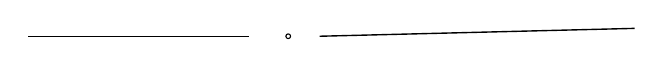
\begin{tikzpicture}[x=1mm,y=1mm]
\draw[line width=.5pt](0,0)--(28,0);
\draw[line width=.5pt](37,0)--(77,1);
\draw[line width=.4pt](33,0)circle(.3);
\end{tikzpicture}}\end{center}
\begin{equation*}f(z)=\sum_\alpha(-1)^{F(\alpha)}e^{-\frac\pi2H(\alpha,\alpha)+\pi H(\alpha,z)}=0=c\Theta(z).\end{equation*}
\Unclear{GELFAND-P000359}{theta-final-argument}{В показателе передано $H(\alpha,z)$. У перечёркнутого $z$ не различима отдельная верхняя черта; предварительное $H(\alpha,\bar z)$ не принято.}
\end{GelfandAdjacentEvidence}
\begin{GelfandAdjacentEvidence}{GELFAND-P000359}{5}

\Unclear{GELFAND-P000359}{zero-theta}{Буквально написано $=0=c\Theta(z)$. Последний аргумент $\Theta$ многократно наведён, с наложенными верхними и нижними штрихами. Условно передано $z$; прежний знак и отдельная верхняя черта не установлены.}
\end{GelfandAdjacentEvidence}
\begin{GelfandAdjacentEvidence}{GELFAND-P000359}{6}




\SourceFigure{GELFAND-P000359}{F-count-insertion}{\par\smallskip\centering{\color{black}\GelfandFitDiagram{\begin{minipage}{148mm}\raggedright \GelfandFitDiagram{\begin{tikzpicture}
\node[inner sep=0](choices)at(0,0){для нек-рых $F(\alpha)$};
\node[anchor=west,inner sep=0](zero)at([xshift=6mm]choices.east){$c=0$.};
\node[inner sep=0]at([xshift=2mm,yshift=8mm]zero.north){--- их \uline{$4^N$}};
\end{tikzpicture}}\end{minipage}}}\par\smallskip }
\end{GelfandAdjacentEvidence}

$c\ne0$ --- Новое предст. $\Theta$-ф-и.
Для половины $F(\alpha)$ это $0$.
$\Theta(z)$ --- станд. ф-я, $\ne0$.
\uline{След. засед. 1-й понед. сентября.}


\Needspace{7\baselineskip}
\begin{GelfandAdjacentEvidence}{GELFAND-P000360}{1}
\SourcePage{GELFAND-P000360}{22}
\uuline{Кириллов} \uwave{с квантованием}. (Костант и т.д.)
\uline{Тривиальная} \uline{часть.}
Симплектич. мн-зие --- $X^{2n}$ --- чётномерное с невыр. замкнутой 2-формой $\omega$ ($d\omega=0$).



\SourceFigure{GELFAND-P000360}{pq-insertion}{\par\smallskip\centering{\color{black}\GelfandFitDiagram{\begin{minipage}{68mm}\raggedright \GelfandFitDiagram{\begin{tikzpicture}
\node[inner sep=0](words)at(0,0){Лок. сущ. такие коорд.};
\node[anchor=west,inner sep=0](that)at([xshift=5mm]words.east){что};
\node[inner sep=0](pq)at([xshift=2mm,yshift=9mm]that.north west){$p\ q$};
\draw[line width=.5pt]([xshift=-2mm,yshift=1mm]pq.west)..controls([xshift=-2mm,yshift=3mm]pq.north west)and([xshift=2mm,yshift=3mm]pq.north east)..([xshift=3mm,yshift=1mm]pq.east)..controls([xshift=3mm,yshift=-2mm]pq.east)and([xshift=1mm,yshift=-2mm]pq.south east)..([xshift=-1mm,yshift=-2mm]pq.south)..controls([xshift=-2mm,yshift=1mm]that.west)and([xshift=-2mm,yshift=-1mm]that.west)..([xshift=-2mm,yshift=-1mm]that.west)..controls([xshift=-2mm,yshift=-2mm]pq.south west)and([xshift=-2mm,yshift=-1mm]pq.west)..([xshift=-2mm,yshift=1mm]pq.west);
\end{tikzpicture}}\end{minipage}}}\par\smallskip }
\end{GelfandAdjacentEvidence}

\begin{equation*}\omega=\sum_{i=1}^n dp_i\wedge dq_i.\end{equation*}
(см. Рашевский «Геом. теор. дифф. ур-й», Стернберг «Лекции по дифф. геом.»).
Объём
\begin{equation*}\Omega=\frac1{n!}\omega\wedge\omega\wedge\cdots\wedge\omega=\frac1{n!}\omega^n\quad(\text{внешн. степ.}).\end{equation*}
\begin{center}\GelfandFitDiagram{\begin{tikzpicture}
\node[inner sep=0](statement)at(0,0){Кас. пр-во отожд. с кокас. с пом. формы $\omega$.};
\draw[line width=.5pt]([xshift=-2mm,yshift=1mm]statement.south west)--([xshift=-2mm,yshift=-2mm]statement.south west)--([xshift=2mm,yshift=-2mm]statement.south east)--([xshift=2mm,yshift=1mm]statement.south east);
\end{tikzpicture}}\end{center}



\begin{GelfandAdjacentEvidence}{GELFAND-P000360}{2}
\begin{equation*}\omega(\xi,\eta)\text{:---}\quad\omega:T_xX\to T_x^*X\quad(\text{изоморфизм}).\end{equation*}
\Unclear{GELFAND-P000360}{tangent-index}{Нижний индекс первого $T$ сильно переписан. Условно передано $x$ с наложенными верхними штрихами; $*$ остаётся кандидатом.}
\end{GelfandAdjacentEvidence}

\begin{equation*}\xi\to\alpha_\xi;\end{equation*}
\begin{center}\GelfandFitDiagram{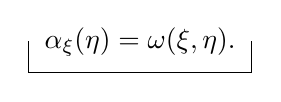
\begin{tikzpicture}
\node[inner sep=0](definition)at(0,0){$\displaystyle\alpha_\xi(\eta)=\omega(\xi,\eta).$};
\draw[line width=.5pt]([xshift=-2mm,yshift=2mm]definition.south west)--([xshift=-2mm,yshift=-2mm]definition.south west)--([xshift=2mm,yshift=-2mm]definition.south east)--([xshift=2mm,yshift=2mm]definition.south east);
\end{tikzpicture}}\end{center}



\begin{equation*}\left(\text{в тех коорд. }\frac{\partial}{\partial q_i}\to dp_i,\quad\frac{\partial}{\partial p_i}\to-dq_i\right).\end{equation*}
Замкн. 1-формы $\leftrightarrow$ вект. поля, сохр. форму $\omega$.
\begin{flushright}в смысле производной Ли $L_\xi$.\end{flushright}
$L_\xi$ действ. на все геом. объекты на мн-зии.
$\varphi_t$ --- соотв. однопар. группа, соотв. полю $\xi$. ($\dot x=\xi(x)$).
\begin{equation*}\left.\frac d{dt}\right|_{t=0}=L_\xi.\end{equation*}
Он перестан. с дифф. дифф. форм: $L_\xi d=dL_\xi$.
$L_\xi f=\xi f$, $L_\xi\eta=[\xi,\eta]$.
\begin{center}\fbox{$L_\xi\omega=0\ \Leftrightarrow\ d\alpha_\xi=0$}\end{center}



--- короткая формулировка.
Такие поля --- \uline{гамильтоновы}, формы --- \uline{градиентные}.
$\xi$ --- лок. гамильт. $\Leftrightarrow\alpha_\xi=df$.
$f$ опр. с точн. до const и многозначно.


\Needspace{7\baselineskip}
\begin{GelfandAdjacentEvidence}{GELFAND-P000361}{1}
\SourcePage{GELFAND-P000361}{unlabelled}



\Unclear{GELFAND-P000361}{hamiltonian-first-mark}{Возле первого $\xi_F$ плотный круглый переписанный знак. Он показан круглой меткой без присвоения математического смысла; точный прежний знак не установлен.\par\smallskip\centering{\color{black}\GelfandFitDiagram{\begin{minipage}{68mm}\raggedright \GelfandFitDiagram{\begin{tikzpicture}
\node[inner sep=0](function)at(0,0){$F$};
\node[inner sep=0](field)at(30mm,0){$\xi_F$};
\draw[->,line width=.5pt]([xshift=2mm]function.east)--([xshift=-2mm]field.west);
\draw[line width=.5pt]([yshift=-2mm]function.south)--([yshift=-5mm]function.south);
\node[anchor=north,inner sep=0]at([yshift=-7mm]function.south){ф-я};
\fill([xshift=-1.4mm,yshift=-.6mm]field.north east)circle(.65mm);
\end{tikzpicture}}\end{minipage}}}\par\smallskip }
\end{GelfandAdjacentEvidence}
\begin{GelfandAdjacentEvidence}{GELFAND-P000361}{2}

$dF$ --- форма $\longleftrightarrow$ гамильт. поле; $dF=2\alpha_{\xi_F}$.
Скобка Пуассона.
\begin{equation*}\{F_1,F_2\}=\xi_{F_1}F_2=-\xi_{F_2}F_1=2\omega(\xi_{F_1},\xi_{F_2}).\end{equation*}
\uline{Тождество}:
\begin{equation*}\xi_{\{F_1,F_2\}}=[\xi_{F_1},\xi_{F_2}].\end{equation*}
\uline{Замечание}:



\Unclear{GELFAND-P000361}{wedge-mark}{Между $(dp\wedge dq)$ и скобкой с векторами плотный перечёркнутый решёткообразный знак. Его штрихи показаны без математического истолкования.\par\smallskip\centering{\color{black}\GelfandFitDiagram{\begin{minipage}{148mm}\raggedright \GelfandFitDiagram{\begin{tikzpicture}
\node[inner sep=0](form)at(0,0){$\displaystyle(dp\wedge dq)$};
\coordinate(mark)at([xshift=4mm]form.east);
\draw[line width=.6pt]([xshift=-1.5mm,yshift=-1mm]mark)--([xshift=-.5mm,yshift=1.2mm]mark);
\draw[line width=.6pt]([xshift=-.3mm,yshift=-1.2mm]mark)--([xshift=.4mm,yshift=1.3mm]mark);
\draw[line width=.6pt]([xshift=.8mm,yshift=-1mm]mark)--([xshift=1.4mm,yshift=1.1mm]mark);
\draw[line width=.6pt]([xshift=-1.8mm,yshift=.6mm]mark)--([xshift=1.7mm,yshift=.6mm]mark);
\draw[line width=.6pt]([xshift=-1.8mm,yshift=-.6mm]mark)--([xshift=1.7mm,yshift=-.6mm]mark);
\node[anchor=west,inner sep=0]at([xshift=4mm]mark){$\displaystyle\left(\frac\partial{\partial p},\frac\partial{\partial q}\right)=\frac12\quad(\text{можно счит. }1).$};
\end{tikzpicture}}\end{minipage}}}\par\smallskip }
\end{GelfandAdjacentEvidence}
\begin{GelfandAdjacentEvidence}{GELFAND-P000361}{3}

\begin{equation*}\frac12[\alpha_1(\xi)\alpha_2(\eta)-\alpha_2(\xi)\alpha_1(\eta)]=\alpha_1\wedge\alpha_2.\end{equation*}
\uline{Новый объект} стр. когда $[\omega]\in H^2(X,Z)$.
Стр. компл. 1-мерное расслоение и отобр. $C$.



\SourceFigure{GELFAND-P000361}{bundle-diagram}{\par\smallskip\centering{\color{black}\GelfandFitDiagram{\begin{minipage}{68mm}\raggedright \begin{equation*}\GelfandFitDiagram{\begin{tikzcd}[ampersand replacement=\&,ampersand replacement=\&]C\arrow[r]\&L\arrow[d]\\\&X\end{tikzcd}}\end{equation*}\end{minipage}}}\par\smallskip }
\end{GelfandAdjacentEvidence}
\begin{GelfandAdjacentEvidence}{GELFAND-P000361}{4}

$\{U_j\}$ --- покрытие, $\omega=d\alpha_j$ в $U_j$.
В $U_j\cap U_k$ стр. $\alpha_j-\alpha_k=df_{jk}$.
\sout{$\alpha$}[?]
\Incomplete{GELFAND-P000361}{cancelled-cocycle}{После $df_{jk}$ начало зачёркнутой записи условно передано $\alpha$. Малые знаки, нижние индексы и продолжение не восстановлены целиком.}
\end{GelfandAdjacentEvidence}
\begin{GelfandAdjacentEvidence}{GELFAND-P000361}{5}

в $U_j\cap U_k\wedge U_\ell$ имеем $d(f_{jk}+f_{k\ell}+f_{\ell j})=0$ и отсюда
\Unclear{GELFAND-P000361}{triple-overlap-wedge}{Второй знак между множествами заострён: условно передано $\wedge$, без замены на обычное пересечение.}
\end{GelfandAdjacentEvidence}
\begin{GelfandAdjacentEvidence}{GELFAND-P000361}{6}




\SourceFigure{GELFAND-P000361}{constant-caption}{\par\smallskip\centering{\color{black}\GelfandFitDiagram{\begin{minipage}{148mm}\raggedright \GelfandFitDiagram{\begin{tikzpicture}
\node[inner sep=0](sum)at(0,0){$\displaystyle f_{jk}+f_{k\ell}+f_{\ell j}=$};
\node[anchor=west,inner sep=0](constant)at([xshift=2mm]sum.east){$\displaystyle C_{jk\ell}$};
\draw[line width=.5pt]([yshift=-1mm]constant.south west)--([yshift=-1mm]constant.south east);
\node[anchor=north,inner sep=0]at([yshift=-3mm]constant.south){const};
\node[anchor=west,inner sep=0]at([xshift=5mm]constant.east){--- 2-мерн. коцикл. Чеха,};
\end{tikzpicture}}\end{minipage}}}\par\smallskip }
\end{GelfandAdjacentEvidence}

соотв. форме \uuline{$\omega$}.
Целочисл. --- $\exists\alpha_j,f_{jk}$, так что $C_{jk\ell}$ --- целочисл.
\begin{equation*}g_{jk}=e^{2\pi if_{jk}}\text{ --- набор ф-й перех. расслоения}\quad(\text{1-мерного}).\end{equation*}
\begin{center}\GelfandFitDiagram{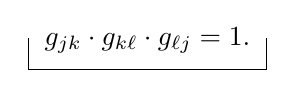
\begin{tikzpicture}
\node[inner sep=0](transition)at(0,0){$\displaystyle g_{jk}\cdot g_{k\ell}\cdot g_{\ell j}=1.$};
\draw[line width=.5pt]([xshift=-2mm,yshift=2mm]transition.south west)--([xshift=-2mm,yshift=-2mm]transition.south west)--([xshift=2mm,yshift=-2mm]transition.south east)--([xshift=2mm,yshift=2mm]transition.south east);
\end{tikzpicture}}\end{center}





\Needspace{7\baselineskip}
\begin{GelfandAdjacentEvidence}{GELFAND-P000362}{1}
\SourcePage{GELFAND-P000362}{23}
Выберем другие $\alpha$,
\sout{[?] const [?]}
\Incomplete{GELFAND-P000362}{cancelled-opening}{В зачёркнутом продолжении условно передан const-подобный фрагмент. Остальные слова и знаки среди длинных петлеобразных зачёркиваний не прочитаны целиком.}
\end{GelfandAdjacentEvidence}

Класс эквив. постр. рассл. зав. от выб. элем.
\begin{center}\GelfandFitDiagram{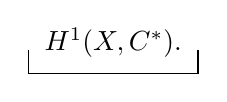
\begin{tikzpicture}
\node[inner sep=0](class)at(0,0){$H^1(X,\mathbb C^*)$.};
\draw[line width=.5pt]([xshift=-2mm,yshift=1mm]class.south west)--([xshift=-2mm,yshift=-2mm]class.south west)--([xshift=2mm,yshift=-2mm]class.south east)--([xshift=2mm,yshift=1mm]class.south east);
\end{tikzpicture}}\end{center}



\begin{GelfandAdjacentEvidence}{GELFAND-P000362}{2}
$H^1(X,\mathbb C^*)$ действ. просто транзит. на мн-ве рассл.
($\mathbb C^*$, а не
\Incomplete{GELFAND-P000362}{cancelled-sheaf}{Малый зачёркнутый токен перед «пучок» целиком не прочитан.}
\end{GelfandAdjacentEvidence}

пучок непр. ф-й.)
$s_j$ в $U_j$, $s_j=g_{jk}s_k$ --- сечение расслоения.



\begin{GelfandAdjacentEvidence}{GELFAND-P000362}{3}
вдоль вект. поля.
\SourceFigure{GELFAND-P000362}{derivative-outline}{\par\smallskip\centering{\color{black}\GelfandFitDiagram{\begin{minipage}{148mm}\raggedright \GelfandFitDiagram{\begin{tikzpicture}
\node[inner sep=0](prefix)at(0,0){\uline{Связность} ---};
\node[anchor=west,inner sep=0](derivative)at([xshift=4mm]prefix.east){производная};
\node[anchor=west,inner sep=0]at([xshift=4mm]derivative.east){сеч.};
\draw[line width=.5pt]([xshift=-2mm]derivative.west)..controls([xshift=-1mm,yshift=4mm]derivative.north west)and([xshift=1mm,yshift=3mm]derivative.north east)..([xshift=2mm,yshift=2mm]derivative.east)..controls([xshift=3mm,yshift=-3mm]derivative.east)and([xshift=1mm,yshift=-3mm]derivative.south east)..([xshift=-1mm,yshift=-2mm]derivative.south west)--([xshift=-2mm]derivative.west);
\draw[line width=.5pt]([xshift=1mm,yshift=3mm]derivative.north east)--([xshift=3mm,yshift=2mm]derivative.north east);
\draw[line width=.5pt]([xshift=1mm,yshift=2mm]derivative.north east)--([xshift=3mm,yshift=3mm]derivative.north east);
\end{tikzpicture}}\end{minipage}}}\par\smallskip }
\end{GelfandAdjacentEvidence}
\begin{GelfandAdjacentEvidence}{GELFAND-P000362}{4}




\Unclear{GELFAND-P000362}{nabla-domain}{У первой $\Gamma$ малый верхний знак утолщён. Условно передано $\Gamma^1(L)$; $\Gamma'(L)$ остаётся кандидатом. Под $\nabla_\xi$ дугообразное подчёркивание.\par\smallskip\centering{\color{black}\GelfandFitDiagram{\begin{minipage}{68mm}\raggedright \GelfandFitDiagram{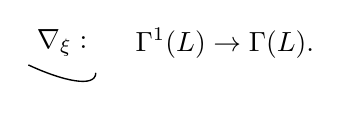
\begin{tikzpicture}
\node[inner sep=0](nabla)at(0,0){$\displaystyle\nabla_\xi:$};
\node[anchor=west,inner sep=0]at([xshift=6mm]nabla.east){$\displaystyle\Gamma^1(L)\to\Gamma(L).$};
\draw[line width=.5pt]([xshift=-1mm,yshift=-1mm]nabla.south west)..controls([yshift=-3mm]nabla.south)and([xshift=1mm,yshift=-4mm]nabla.south east)..([xshift=1mm,yshift=-2mm]nabla.south east);
\end{tikzpicture}}\end{minipage}}}\par\smallskip }
\end{GelfandAdjacentEvidence}
\begin{GelfandAdjacentEvidence}{GELFAND-P000362}{5}




\SourceFigure{GELFAND-P000362}{choice-marginal}{\par\smallskip\centering{\color{black}\GelfandFitDiagram{\begin{minipage}{68mm}\raggedright \begin{flushright}\GelfandFitDiagram{\begin{tikzpicture}[x=1mm,y=1mm]
\node[anchor=west,inner sep=0]at(0,0){\uline{Выбор}};
\node[anchor=west,inner sep=0](choice)at(0,-7){$\alpha_j$ зад. связность.};
\draw[line width=.5pt]([yshift=-1mm]choice.south west)--([yshift=-1mm]choice.south east);
\draw[line width=.5pt](-4,3)--(-5,-15);
\draw[line width=.5pt](-7,3)--(-8,-17);
\end{tikzpicture}}\end{flushright}\end{minipage}}}\par\smallskip }
\end{GelfandAdjacentEvidence}

\begin{center}\GelfandFitDiagram{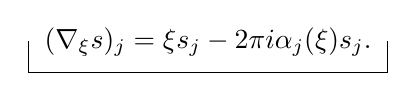
\begin{tikzpicture}
\node[inner sep=0](connection)at(0,0){$\displaystyle(\nabla_\xi s)_j=\xi s_j-2\pi i\alpha_j(\xi)s_j.$};
\draw[line width=.5pt]([xshift=-2mm,yshift=2mm]connection.south west)--([xshift=-2mm,yshift=-2mm]connection.south west)--([xshift=2mm,yshift=-2mm]connection.south east)--([xshift=2mm,yshift=2mm]connection.south east);
\end{tikzpicture}}\end{center}



\begin{GelfandAdjacentEvidence}{GELFAND-P000362}{6}
Это действ. опер. в пр-ве сечений. (проверка предост. чит.).
\Unclear{GELFAND-P000362}{reader-proof-note}{Первое слово условно прочитано «проверка»; «проверить» остаётся кандидатом. Далее «предост. чит.» с отдельной о-подобной петлёй после д. Сокращения в русской записи не раскрыты.}
\end{GelfandAdjacentEvidence}
\begin{GelfandAdjacentEvidence}{GELFAND-P000362}{7}

\uline{Проверить}:
\begin{equation*}(\nabla_\xi s)_j=g_{jk}(\nabla_\xi s)_k.\end{equation*}
Опр. эрмитово рассл. со связностью и в нём обобщ. преобр. Фурье.
Рассм. произв. дифф. опер. 1-го пор. в рассл. $L$.
\begin{equation*}D:\Gamma(L)\to\Gamma(L)\quad(\text{в лок. коорд. обычн.}).\end{equation*}
Общ. вид его: $D=\nabla_\xi+\varphi=D_{\xi,\varphi}$ ($\varphi$ --- опер. умн. на ф-ю).



\Incomplete{GELFAND-P000362}{compatible-cancelled}{Прежнее прилагательное зачёркнуто и не восстановлено целиком. Над ним вставлено и обведено читаемое «согласованным».\par\smallskip\centering{\color{black}\GelfandFitDiagram{\begin{minipage}{148mm}\raggedright \GelfandFitDiagram{\begin{tikzpicture}
\node[inner sep=0](prefix)at(0,0){$D$ наз.};
\node[anchor=west,inner sep=0](old)at([xshift=5mm]prefix.east){[?]};
\draw[line width=.5pt]([xshift=-1mm,yshift=.5mm]old.west)--([xshift=1mm,yshift=.5mm]old.east);
\draw[line width=.5pt]([xshift=-1mm,yshift=-.5mm]old.west)--([xshift=1mm,yshift=-.5mm]old.east);
\node[inner sep=0](new)at([xshift=10mm,yshift=9mm]old.north){согласованным};
\draw[line width=.5pt]([xshift=-2mm,yshift=1mm]new.west)..controls([xshift=-2mm,yshift=3mm]new.north west)and([xshift=2mm,yshift=3mm]new.north east)..([xshift=3mm,yshift=1mm]new.east)..controls([xshift=3mm,yshift=-2mm]new.east)and([xshift=2mm,yshift=-2mm]new.south east)..([xshift=-2mm,yshift=-2mm]new.south west)..controls([xshift=-1mm,yshift=1mm]old.west)and([xshift=-1mm,yshift=-1mm]old.west)..([xshift=-1mm,yshift=-1mm]old.west)..controls([xshift=-2mm,yshift=3mm]old.west)and([xshift=-3mm,yshift=-1mm]new.west)..([xshift=-2mm,yshift=1mm]new.west);
\node[anchor=west,inner sep=0]at([xshift=5mm]old.east){со связностью, если};
\end{tikzpicture}}\end{minipage}}}\par\smallskip }
\end{GelfandAdjacentEvidence}
\begin{GelfandAdjacentEvidence}{GELFAND-P000362}{8}




\SourceFigure{GELFAND-P000362}{right-commutator-arrow}{Дуга начинается справа от коммутатора, выгибается вправо вдоль замечаний в квадратных скобках и заканчивается вниз-влево над нижней рамкой. Дополнительное математическое отношение этой дуге не приписано.\par\smallskip\centering{\color{black}\GelfandFitDiagram{\begin{minipage}{148mm}\raggedright \GelfandFitDiagram{\begin{tikzpicture}[x=1mm,y=1mm]
\node[inner sep=0](commutator)at(0,0){$\displaystyle[D_{\xi,\varphi},\nabla_\eta]=\nabla_{[\xi,\eta]}.$};
\draw[line width=.5pt]([xshift=-2mm,yshift=2mm]commutator.south west)--([xshift=-2mm,yshift=-2mm]commutator.south west)--([xshift=2mm,yshift=-2mm]commutator.south east)--([xshift=2mm,yshift=2mm]commutator.south east);
\node[anchor=north,inner sep=0,align=left,text width=115mm](curvature)at(0,-13){$\omega$ --- форма кривизны этой связности.\\Она всегда замкн., но не всегда невырожд.};
\draw[line width=.5pt]([xshift=-1mm,yshift=1mm]curvature.north west)--([xshift=-3mm,yshift=1mm]curvature.north west)--([xshift=-3mm,yshift=-1mm]curvature.south west)--([xshift=-1mm,yshift=-1mm]curvature.south west);
\draw[line width=.5pt]([xshift=1mm,yshift=1mm]curvature.north east)--([xshift=3mm,yshift=1mm]curvature.north east)--([xshift=3mm,yshift=-1mm]curvature.south east)--([xshift=1mm,yshift=-1mm]curvature.south east);
\node[anchor=north west,inner sep=0]at(-57.5,-31){[Связн. --- 1-форма со знач. в $L$.]};
\draw[->,line width=.5pt](45,0)..controls(90,-7)and(90,-25)..(45,-40);
\end{tikzpicture}}\end{minipage}}}\par\smallskip }
\end{GelfandAdjacentEvidence}
\begin{GelfandAdjacentEvidence}{GELFAND-P000362}{9}

Или
\begin{center}\fbox{$\xi=\frac1{\pi i}\xi_\varphi$}\end{center}
\Unclear{GELFAND-P000362}{normalization}{В рамке буквально написано $\xi=\frac1{\pi i}\xi_\varphi$.}
\end{GelfandAdjacentEvidence}

(в частн., $\xi$ наст. гамильтоново.)


\Needspace{7\baselineskip}
\begin{GelfandAdjacentEvidence}{GELFAND-P000363}{1}
\SourcePage{GELFAND-P000363}{unlabelled}
\sout{$D_\varphi$}
\Unclear{GELFAND-P000363}{cancelled-initial}{Зачёркнутый начальный знак условно передан $D_\varphi$; перекрытые штрихи не дают уверенного чтения.}
\end{GelfandAdjacentEvidence}
\begin{GelfandAdjacentEvidence}{GELFAND-P000363}{2}

Оператор $D_\varphi=\nabla_{\xi_\varphi}+\pi i\varphi:\Gamma(L)\to\Gamma(L)$.
\uline{Осн. теорема}:
\begin{equation*}[D_\varphi,D_\psi]=D_{\{\varphi,\psi\}}.\end{equation*}
(получ. предст. алгебры Ли) соглас. со связностью.
(предст. Ван Хова: ф-ии $\to$ опер. в сеч. расслоения) соглас. со связностью.
\uwave{Это наз. предквантованием}.



\SourceFigure{GELFAND-P000363}{prequant-margin-arrow}{Перед правой пометой короткая стрелка влево со штрихом справа. Точная конечная точка не установлена; дополнительная логическая связь не приписана.\par\smallskip\centering{\color{black}\GelfandFitDiagram{\begin{minipage}{148mm}\raggedright \begin{flushright}$\leftarrow$ действ. в слишком широком пр-ве.\end{flushright}\end{minipage}}}\par\smallskip }
\end{GelfandAdjacentEvidence}

(\sout{Это.} рассм. 200 стр. 3-й вып. Лекц. по совр. ан., Lecture Notes,
\uwave{Lectures on Modern Analysis}, $\overline{\underline{\mathrm{III}}}$).
\uline{Лагранжево} \uline{распределение} (изотропное пр-во) ---
--- в $\forall$ точке зад. лагр. подпр-во. $\frac12$ разм.
\begin{equation*}F:F_x\subset T_*X,\qquad\omega|_{F_x}=0,\qquad\dim F_x=n=\frac12\dim X.\end{equation*}
Будут рассм. компл. распр.:
\begin{equation*}F_x\subset T_x^CX,\qquad\omega|_{F_x}=0,\qquad\dim_C F_x=n=\frac12\dim X.\end{equation*}
Выбор интегр. лагр. распр. --- \uuline{поляризацией}.



\begin{GelfandAdjacentEvidence}{GELFAND-P000363}{3}
Оно счит. интегрируемым (усл. Фробениуса) --- см. \uline{Дьедонне}.
(Локально сущ. --- из-за $\sum dp\wedge dq$) взять $p$-подпр-во.



\SourceFigure{GELFAND-P000363}{complex-marginal}{\par\smallskip\centering{\color{black}\GelfandFitDiagram{\begin{minipage}{68mm}\raggedright \begin{flushright}\GelfandFitDiagram{\begin{tikzpicture}[x=1mm,y=1mm]
\node[anchor=west,inner sep=0]at(0,0){Комплексное тяжело.};
\draw[line width=.5pt](-4,3)--(-5,-10);
\draw[line width=.5pt](-7,3)--(-8,-11);
\end{tikzpicture}}\end{flushright}\end{minipage}}}\par\smallskip }
\end{GelfandAdjacentEvidence}

\uline{Пример}: сфера с обычн. объёмом. Глоб. нельзя.
\uline{Частн. случаи} (крайнии).

\begin{GelfandAdjacentEvidence}{GELFAND-P000363}{4}
1) $\overline{\boldsymbol F}_x=F_x$ --- вещ. распределение. (\uline{вещ. поляриз.})
\Unclear{GELFAND-P000363}{real-polarization-overwrite}{В первом равенстве первое $F$ и черта сильно утолщены или переписаны. Нынешнее чтение условно передано $\bar F_x=F_x$; прежние штрихи не отделены.}
\end{GelfandAdjacentEvidence}

2) $F_x\cap\bar F_x=0.$ (кэлерова \uline{поляризация}).
\begin{equation*}\dim(F_x+\bar F_x)=k\quad(=\mathrm{const})\quad(\text{и интегр. рассл.}).\end{equation*}
Там есть структ. смешанного мн. (рассл. в вещ. базой и компл. слоями; перех. --- голом. преобр. слоёв).


\Needspace{7\baselineskip}
\begin{GelfandAdjacentEvidence}{GELFAND-P000364}{1}
\SourcePage{GELFAND-P000364}{24}
$F$ --- распр., $\Gamma(L,F)$ --- сеч., пост. вдоль слоёв, т.е. $\nabla_\xi s=0$ если $\xi_x\in F_x$.
Теперь действие опр. рассм. на \uuline{$\Gamma(L,F)$}.



\SourceFigure{GELFAND-P000364}{algebra-caption}{\par\smallskip\centering{\color{black}\GelfandFitDiagram{\begin{minipage}{148mm}\raggedright \GelfandFitDiagram{\begin{tikzpicture}
\node[inner sep=0](algebra)at(0,0){$A(F)$};
\draw[line width=.5pt]([yshift=-1mm]algebra.south west)--([yshift=-1mm]algebra.south east);
\node[anchor=west,inner sep=0]at([xshift=4mm]algebra.east){--- ф-ии $\varphi$, пост. вдоль слоёв.};
\draw[line width=.5pt]([yshift=-3mm]algebra.south)--([yshift=-6mm]algebra.south);
\node[anchor=north,inner sep=0,align=left]at([xshift=6mm,yshift=-8mm]algebra.south){алгебра\\таких ф-й.};
\end{tikzpicture}}\end{minipage}}}\par\smallskip }
\end{GelfandAdjacentEvidence}
\begin{GelfandAdjacentEvidence}{GELFAND-P000364}{2}

($\xi f=0$, \sout{$\forall$}
\Unclear{GELFAND-P000364}{cancelled-forall}{Зачёркнутый знак условно передан $\forall$; его пересекают наложенные диагональные штрихи.}
\end{GelfandAdjacentEvidence}
\begin{GelfandAdjacentEvidence}{GELFAND-P000364}{3}

если $\xi_x\in F_x$).
$\varphi\in A(F)\Rightarrow D_\varphi$ сохр. пр-во сечений ($D_\varphi$ действ. в $\Gamma(L,F)$ как умн. на $\varphi$).
\uwave{$A(F)$ --- макс. коммут. подалг. со скобкой Пуассона} (локально).
Рассм. теперь операторы (тоже сохр. $\Gamma(L,F)$)
\begin{equation*}\begin{aligned}A_1(F)&=\text{нормализ. }A(F)\text{ в алг. скобок Пуасс.}=\\&=\{\varphi:\{\varphi,A(F)\}\subset A(F)\}.\end{aligned}\end{equation*}
\uuline{Теор.} Опер. $D_\varphi$ с $\varphi\in A_1(F)$ сохр. $\Gamma(L,F)$ и действ. там как опер. 1-го пор.
Это уже \uline{квантование}, а ф-ии --- квантующие.
(Другие квант. уже неоднозначно).
\textbf{и}х много.
\Unclear{GELFAND-P000364}{overwritten-their}{Нынешнее «их» читается, но первый знак переписан. Прежние штрихи не разделены.}
\end{GelfandAdjacentEvidence}

$p,q$; $dq=0$ --- подпр., ф-ии --- только от $q$.
\uline{Опер.} --- ф-ии от $q$ --- опер. умн., лин. ф-ии от $p$ --- опер. 1-го пор.
\begin{center}\GelfandFitDiagram{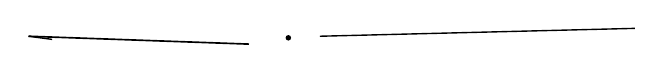
\begin{tikzpicture}[x=1mm,y=1mm]
\draw[line width=.6pt](0,0)--(28,-1);
\draw[line width=.5pt](0,0)--(3,-.4);
\draw[line width=.5pt](37,0)--(77,1);
\fill(33,-.2)circle(.35);
\end{tikzpicture}}\end{center}
\uline{След. раз}: \uuline{Кириллов.}


\Needspace{7\baselineskip}
\begin{GelfandAdjacentEvidence}{GELFAND-P000365}{1}
\SourcePage{GELFAND-P000365}{unlabelled}
\uuline{13/$\overline{\underline{\mathrm{IX}}}$-71 г.}
\uuline{И. М. Гельфанд} \uuline{о} \uuline{раб.} \uuline{Спрингера} (выч. хар. для полупр. групп над кон. полем).
1. \uwave{Рассмотрим} \uwave{гр.} $SL(n,C)$ и унипот. матр. [?]
\Unclear{GELFAND-P000365}{uni-prefix}{Перед первой матрицей отдельный тёмный переписанный знак. Надёжное чтение $U$ или равенства не установлено.}
\end{GelfandAdjacentEvidence}
\begin{GelfandAdjacentEvidence}{GELFAND-P000365}{2}

\begin{equation*}\begin{pmatrix}1&&&0\\&1&&\\&&\ddots&\\\dots&&&1\end{pmatrix}\end{equation*}
\sout{$U$}[?]
\Incomplete{GELFAND-P000365}{uni-cancel}{В начале короткой зачёркнутой записи условно передан $U$-подобный знак. Остальные знаки под горизонталями не прочитаны целиком.}
\end{GelfandAdjacentEvidence}
\begin{GelfandAdjacentEvidence}{GELFAND-P000365}{3}

(прив. к так. виду). $(1+a,\ \text{где }a^n=0)$.
В $1$ --- особ. точки.
\begin{equation*}\begin{pmatrix}a&b\\c&d\end{pmatrix},\quad ad-bc=1,\qquad\text{унипот. }a+d=2,\quad\text{в }R^3\text{ конус,}\quad1\text{ --- особенность.}\end{equation*}
\uuline{Неособые} --- одна жорд. клетка.
\uwave{Неск. жорд. клеток} --- \textbf{особые}.
\uline{Ответ}: $R$ --- мн-во



\Incomplete{GELFAND-P000365}{answer-cancel}{Под обведённой вставкой «всех унипот. матриц» прежняя фраза зачёркнута. Её остаток между и после условно читаемых фрагментов не восстановлен.\par\smallskip\centering{\color{black}\GelfandFitDiagram{\begin{minipage}{148mm}\raggedright \GelfandFitDiagram{\begin{tikzpicture}
\node[inner sep=0](old)at(0,0){\sout{матр.[?]\quad[?]\quad особ.[?]\quad[?]},};
\node[anchor=south west,inner sep=0](new)at([yshift=6mm]old.north west){всех унипот. матриц};
\draw[line width=.5pt]([xshift=-2mm,yshift=1mm]new.north west)--([xshift=2mm,yshift=1mm]new.north east)..controls([xshift=6mm,yshift=1mm]new.north east)and([xshift=6mm,yshift=-2mm]new.south east)..([xshift=2mm,yshift=-2mm]new.south east)--([xshift=-1mm,yshift=-2mm]new.south west)..controls([xshift=-4mm,yshift=-3mm]new.south west)and([xshift=-3mm,yshift=-2mm]old.west)..([xshift=-3mm,yshift=-2mm]old.west)--([xshift=-2mm,yshift=1mm]new.north west);
\draw[line width=.6pt]([xshift=-1mm,yshift=-1mm]old.west)--([xshift=1mm,yshift=1mm]old.east);
\end{tikzpicture}}\end{minipage}}}\par\smallskip }
\end{GelfandAdjacentEvidence}
\begin{GelfandAdjacentEvidence}{GELFAND-P000365}{4}

\Unclear{GELFAND-P000365}{answer-cancel-fragments}{В зачёркнутой строке условно переданы сокращения «матр.» и «особ.». Окончания и промежуточная запись закрыты штрихами; сокращения не раскрыты.}
\end{GelfandAdjacentEvidence}
\begin{GelfandAdjacentEvidence}{GELFAND-P000365}{5}

$g\in R$.



\Unclear{GELFAND-P000365}{projective-cancel}{Между $P=$ и $B\backslash G$ густо зачёркнут знак, условно $P$. Точный прежний знак не восстановлен. Под ним короткий вертикальный штрих и подпись «проект. пр-во.».\par\smallskip\centering{\color{black}\GelfandFitDiagram{\begin{minipage}{148mm}\raggedright \GelfandFitDiagram{\begin{tikzpicture}
\node[inner sep=0](prefix)at(0,0){$P=$};
\node[anchor=west,inner sep=0](cancelled)at([xshift=4mm]prefix.east){\sout{$P$}[?]};
\node[anchor=west,inner sep=0]at([xshift=4mm]cancelled.east){$B\backslash G$};
\draw[line width=.5pt]([yshift=-2mm]cancelled.south)--([yshift=-4mm]cancelled.south);
\node[anchor=north,inner sep=0]at([yshift=-6mm]cancelled.south){проект. пр-во.};
\end{tikzpicture}}\end{minipage}}}\par\smallskip }
\end{GelfandAdjacentEvidence}
\begin{GelfandAdjacentEvidence}{GELFAND-P000365}{6}

$B$ --- треуг. матрицы
\begin{equation*}\begin{pmatrix}\lambda_1&&0\\&\ddots&\\\dots&&\lambda_n\end{pmatrix}.\end{equation*}
Рассм. пары $(p,g)$ с действиями
\begin{equation*}pgp^{-1}\in U=\left\{\begin{pmatrix}1&&&0\\&1&&\\&&\ddots&\\\dots&&&1\end{pmatrix}\right\},\qquad p\in P.\end{equation*}
(Это не зав. от выб. предст. эл. из $p$.)
$\bar R$ --- мн-во пар.
\begin{equation*}(p,g)\longrightarrow g.\end{equation*}
Это $\bar R\to R$, разрешение особенностей (всех).
Над точкой общ. полож. \uline{один элемент.}
$\bar R$ --- неособое многообразие.
(Это для произв. \uwave{редукт.} \uwave{группы} на\textbf{д} $\forall$ полем.)
\Unclear{GELFAND-P000365}{reductive-overwritten}{Слово «над» читается, но последняя буква сильно переписана с отдельной дугой сверху. Прежние штрихи не разделены.}
\end{GelfandAdjacentEvidence}
\begin{GelfandAdjacentEvidence}{GELFAND-P000365}{7}

2. \uline{Геом. истолкование полиномов Холла.}
Рассм. $G$ [?]
\Incomplete{GELFAND-P000365}{group-overwrite}{После $G$ короткая переписанная и зачёркнутая группа штрихов. Равенство остаётся кандидатом; уверенное прежнее чтение не установлено.}
\end{GelfandAdjacentEvidence}
\begin{GelfandAdjacentEvidence}{GELFAND-P000365}{8}

--- гр. матриц, $B$ --- гр. треуг. матр.
\begin{equation*}G=GL(n,F_q),\qquad B\backslash G\text{ --- флаги.}\end{equation*}



\SourceFigure{GELFAND-P000365}{flag-sketch-marks}{Наклонный четырёхсторонний контур с почти средней ломаной и крупной точкой на ней. Маленькая отдельная точка над верхним средним соединением, короткий след слева вверху и утолщённый правый верхний стык переданы без присвоения дополнительных узлов или математического смысла.\par\smallskip\centering{\color{black}\GelfandFitDiagram{\begin{minipage}{68mm}\raggedright \GelfandFitDiagram{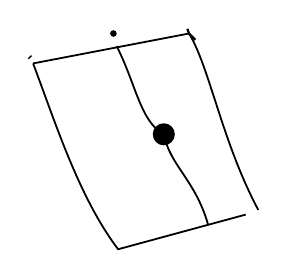
\begin{tikzpicture}[x=.2mm,y=-.2mm]
\draw[line width=.65pt](26,58)--(125,39)..controls(138,60)and(146,108)..(169,151);
\draw[line width=.65pt](26,58)..controls(40,95)and(55,143)..(80,176)--(161,154);
\draw[line width=.65pt](79,47)..controls(91,70)and(94,95)..(109,103)..controls(113,123)and(129,132)..(137,160);
\fill(109,103)circle(7);
\fill(77,39)circle(2.1);
\draw[line width=.8pt](124,36)--(125,39)--(129,43);
\draw[line width=.5pt](23,55)--(25,53);
\end{tikzpicture}}\end{minipage}}}\par\smallskip }
\end{GelfandAdjacentEvidence}

Число флагов --- полином по $q$, степень к-рого зав. от $n$.


\Needspace{7\baselineskip}
\begin{GelfandAdjacentEvidence}{GELFAND-P000366}{1}
\SourcePage{GELFAND-P000366}{25}
Класс смежн. опр. разбиением $n=n_1+\dots+n_k$,
$u\in U$ --- элем. из этого класса.
\begin{equation*}|P^{\boldsymbol{u}}|=P_{n_1,\dots,n_k}(q)\text{ --- полином Холла}\end{equation*}
\uline{(число неподв. точек этого элемента).}
$u=1$ --- получ. полином Пуанкаре.
Это позв. опр. полином Пуанкаре для любой расщеп. группы.
\Unclear{GELFAND-P000366}{allows-abbreviation}{В сокращении после «Это» первый знак похож на $\text{п}$, далее округлый знак и з-подобный нижний ход. Условно передано «позв.»; прежнее чтение «назв.» не принято уверенно. Сокращение в русской записи не раскрыто.}
\end{GelfandAdjacentEvidence}

\begin{center}\GelfandFitDiagram{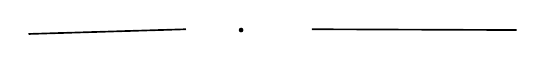
\begin{tikzpicture}[x=1mm,y=1mm]\draw[line width=.6pt](0,0)--(20,.6);\fill(27,.5)circle(.3);\draw[line width=.6pt](36,.6)--(62,.5);\end{tikzpicture}}\end{center}
J. A. Green, Trans. A. M. S., 1955 --- рекомендуется.
\begin{center}\GelfandFitDiagram{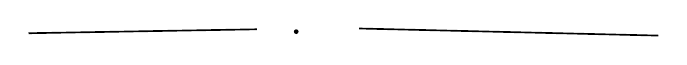
\begin{tikzpicture}[x=1mm,y=1mm]\draw[line width=.6pt](0,0)--(29,.5);\fill(34,.2)circle(.3);\draw[line width=.6pt](42,.6)--(80,-.3);\end{tikzpicture}}\end{center}
Есть оценки разм. мн-зия, леж. при этом над точкой.
\begin{equation*}\pi:\bar R\longrightarrow R,\end{equation*}
\begin{center}\GelfandFitDiagram{\begin{tikzpicture}
\node[inner sep=0](bound)at(0,0){$\displaystyle\dim\pi^{-1}(g)\le\frac{\dim Z_g-(n-1)}2$};
\draw[line width=.5pt]([xshift=-2mm,yshift=2mm]bound.south west)--([xshift=-2mm,yshift=-2mm]bound.south west)--([xshift=2mm,yshift=-2mm]bound.south east)--([xshift=3mm,yshift=3mm]bound.south east);
\node[anchor=north west,inner sep=0](centralizer)at([xshift=4mm,yshift=-6mm]bound.south west){$Z_g$ --- централизатор $g$.};
\draw[line width=.5pt]([xshift=-1mm,yshift=1mm]centralizer.south west)--([xshift=-1mm,yshift=-2mm]centralizer.south west)--([xshift=2mm,yshift=-2mm]centralizer.south east)--([xshift=2mm,yshift=1mm]centralizer.south east);
\end{tikzpicture}}\end{center}



\begin{GelfandAdjacentEvidence}{GELFAND-P000366}{2}
\begin{center}\GelfandFitDiagram{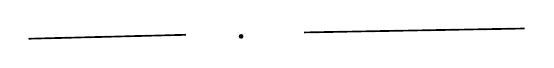
\begin{tikzpicture}[x=1mm,y=1mm]\draw[line width=.6pt](0,0)--(20,.5);\fill(27,.3)circle(.3);\draw[line width=.6pt](35,.8)--(63,1.3);\end{tikzpicture}}\end{center}
\uuline{Б. Розенфельд.}
О заметках \uline{Rego}, C. R., t. 272 (1971).
\sout{В кас. пр-ве.}



\SourceFigure{GELFAND-P000366}{distribution-insertion}{\par\smallskip\centering{\color{black}\GelfandFitDiagram{\begin{minipage}{148mm}\raggedright \GelfandFitDiagram{\begin{tikzpicture}
\node[anchor=west,inner sep=0](prefix)at(0,0){\uwave{Зад. распределение}};
\node[anchor=west,inner sep=0](integrable)at([xshift=36mm]prefix.east){(интегрируемое)};
\node[anchor=west,inner sep=0]at([xshift=4mm]integrable.east){с ним};
\node[inner sep=0](insert)at([xshift=1mm,yshift=10mm]integrable.north east){на $M$};
\draw[line width=.5pt]([xshift=-2mm,yshift=1mm]insert.west)..controls([xshift=-4mm,yshift=2mm]insert.north west)and([xshift=1mm,yshift=5mm]insert.north east)..([xshift=3mm,yshift=1mm]insert.east)..controls([xshift=4mm,yshift=-2mm]insert.east)and([xshift=2mm,yshift=-3mm]insert.south east)..([xshift=1mm,yshift=-2mm]integrable.east)..controls([xshift=2mm,yshift=2mm]integrable.east)and([xshift=-2mm,yshift=-2mm]insert.south west)..([xshift=-2mm,yshift=1mm]insert.west);
\draw[line width=.5pt]([yshift=-2mm]integrable.south)--([yshift=-5mm]integrable.south);
\node[anchor=north,inner sep=0]at([yshift=-7mm]integrable.south){усл. Фробениуса};
\node[anchor=north west,inner sep=0](cohomology)at([yshift=-11mm]prefix.south west){связ. нек-рые когомологии.};
\draw[line width=.6pt]([xshift=4mm,yshift=-1mm]cohomology.south east)--([xshift=4mm,yshift=5mm]cohomology.north east);
\end{tikzpicture}}\end{minipage}}}\par\smallskip }
\end{GelfandAdjacentEvidence}
\begin{GelfandAdjacentEvidence}{GELFAND-P000366}{3}




\Unclear{GELFAND-P000366}{forms-insert-ending}{Над «дифф. форм» вставлено слово, условно «комплексно.». Окончание и сокращение сомнительны; «комплексна.», «комплексн.» и «комплекса.» также остаются кандидатами. Чтение не выбрано по грамматике.\par\smallskip\centering{\color{black}\GelfandFitDiagram{\begin{minipage}{148mm}\raggedright \GelfandFitDiagram{\begin{tikzpicture}
\node[anchor=west,inner sep=0](prefix)at(0,0){Всякое дифф. град. кольца};
\node[anchor=west,inner sep=0](forms)at([xshift=4mm]prefix.east){дифф. форм};
\node[anchor=south west,inner sep=0]at([yshift=2mm]forms.north west){комплексно.[?]};
\node[anchor=west,inner sep=0]at([xshift=4mm]forms.east){на $M$ им. вид};
\end{tikzpicture}}\end{minipage}}}\par\smallskip }
\end{GelfandAdjacentEvidence}
\begin{GelfandAdjacentEvidence}{GELFAND-P000366}{4}

\begin{equation*}d_{L_1}+i_{L_2}\end{equation*}
($i_{L_2}$ --- внутр. умнож. на вектор-форму).
\begin{center}\GelfandFitDiagram{\begin{tikzpicture}[x=1mm,y=1mm]\draw[line width=.45pt,dash pattern=on 2mm off 6mm](0,0)--(137,-2);\end{tikzpicture}}\end{center}
\begin{gather*}
\omega(X_1,\dots,X_q)\text{ --- скал. форма.}\\
L(X_1,\dots,X_p)\text{ --- форма (векторнознач.).}\\
(i_L\omega)(X_1,\dots,X_{p+q-1})\quad\text{подст. и кососимм.}\\
d_L\omega=(d\circ i_L+(-1)^p i_L\circ d)\omega.
\end{gather*}
$L$ --- форма ст. $0$ (вект. поле) --- $d_L$ --- произв. Ли.
\sout{$d_L^2=0$}[?]
\Unclear{GELFAND-P000366}{integrable-cancel}{Перед «интегрируемость» короткая формула зачёркнута. Условно передано $d_L^2=0$; индекс и степень при $d$ скрыты наложением штрихов и не установлены уверенно.}
\end{GelfandAdjacentEvidence}

Интегрируемость. (квадр. $=0$)


\Needspace{7\baselineskip}
\begin{GelfandAdjacentEvidence}{GELFAND-P000367}{1}
\SourcePage{GELFAND-P000367}{unlabelled}
Проф. \uuline{Птак}.
\begin{equation*}\dim E\le\infty,\qquad E\text{ с нормой}.\end{equation*}
\Unclear{GELFAND-P000367}{dimension-sign}{Между $\dim E$ и $\infty$ несколько наложенных наклонных и горизонтальных штрихов. Условно передано $\le$; $<$ и $\ne$ остаются кандидатами.}
\end{GelfandAdjacentEvidence}
\begin{GelfandAdjacentEvidence}{GELFAND-P000367}{2}

$q$ --- показатель (крит.), если
\begin{equation*}1^\circ.\quad A\in L(E),\quad1=|A|=|A^{\boldsymbol{q}}|\Rightarrow|A|_\sigma=1\quad\text{(сп. радиус)}.\end{equation*}
\Unclear{GELFAND-P000367}{a-exponent}{Степень второго $A$ сильно утолщена или переписана. $q$ передано условно; прежний показатель не установлен.}
\end{GelfandAdjacentEvidence}
\begin{GelfandAdjacentEvidence}{GELFAND-P000367}{3}

\begin{equation*}2^\circ.\quad\exists B,\quad1=|B|=|B^{q-1}|,\quad\text{но }|B|_\sigma<1.\end{equation*}
\begin{equation*}\begin{aligned}\ell^\infty\quad&|x|=\max|x_i|,\\\ell_1\quad&\sum|x_i|,\end{aligned}\qquad q(n)=n^2-n+1.\end{equation*}
\begin{equation*}\ell_2\qquad q(n)=n.\end{equation*}
Сущ. $2$-мерн. пр-во, в к-ром $q=\infty$.
(По норме плохо оценивать сходимость нужны соб. знач.).



\SourceFigure{GELFAND-P000367}{danzer-diagram}{\par\smallskip\centering{\color{black}\GelfandFitDiagram{\begin{minipage}{68mm}\raggedright \GelfandFitDiagram{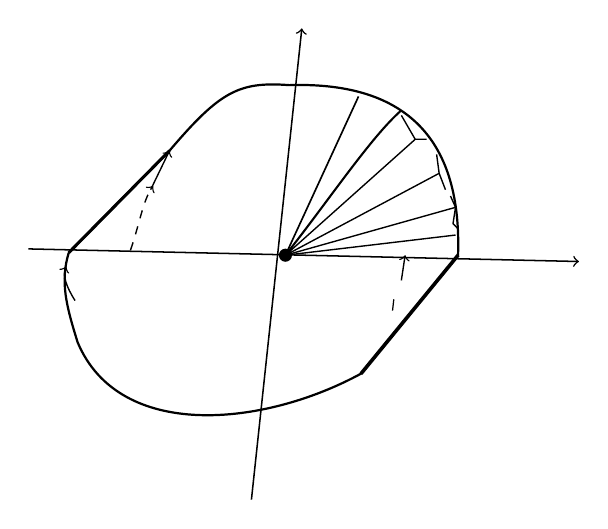
\begin{tikzpicture}[x=.16mm,y=-.16mm]
\draw[line width=.8pt](45,193)--(125,112)..controls(165,65)and(180,57)..(220,60)..controls(315,57)and(357,105)..(354,195)--(277,289)..controls(200,331)and(85,343)..(52,264)..controls(43,235)and(38,216)..(45,193);
\draw[line width=1.1pt](45,193)--(125,112);
\draw[line width=1.3pt](354,195)--(277,289);
\draw[line width=.55pt,->](190,389)--(230,15);
\draw[line width=.55pt,->](13,190)--(450,200);
\fill(217,195)circle(5.2);
\draw[line width=.6pt](217,195)--(275,69);
\draw[line width=.75pt](217,195)..controls(251,152)and(285,101)..(309,80);
\draw[line width=.5pt](217,195)--(320,103);
\draw[line width=.5pt](217,195)--(339,130);
\draw[line width=.5pt](217,195)--(352,157);
\draw[line width=.5pt](217,195)--(352,179);
\draw[line width=.5pt](309,84)--(320,103)--(329,103);
\draw[line width=.5pt](337,115)--(339,130)--(344,143);
\draw[line width=.5pt](348,148)--(352,157)--(350,170)--(354,174);
\draw[line width=.5pt,dashed,->](94,191)..controls(101,171)and(104,151)..(112,140);
\draw[line width=.5pt,->](110,143)--(125,112);
\draw[line width=.5pt,->](50,231)..controls(43,220)and(40,211)..(43,204);
\draw[line width=.5pt,->](309,215)--(312,195);
\draw[line width=.45pt](303,230)--(302,239);
\end{tikzpicture}}\end{minipage}}}\par\smallskip }
\end{GelfandAdjacentEvidence}
\begin{GelfandAdjacentEvidence}{GELFAND-P000367}{4}

$A$ --- поворот на малый угол (пример Danzer'a).
$\ell_p$ --- неизвестно, сущ. ли, кроме $p=2^m$.
\uline{Полезная зад. для вычислит. математики.}
\begin{equation*}M(n)=\min\text{ по всем бан. }\le n.\end{equation*}
\Unclear{GELFAND-P000367}{banach-overwritten}{Сокращение после «по всем» условно передано «бан.». Средние буквы сильно утолщены и переписаны; прежние штрихи не разделены. Сокращение не раскрыто.}
\end{GelfandAdjacentEvidence}
\begin{GelfandAdjacentEvidence}{GELFAND-P000367}{5}

$\exists$ те, по к-рым $<n$!
Сущ. послед. $M(n_k)\sim\sqrt{n_k}$.
Неизвестно, верно ли, что $\liminf M(n)=\infty$.
\begin{equation*}\ell_4^2\underset{\ell_1}{\oplus}\ell_8^2\end{equation*}



\Unclear{GELFAND-P000367}{dimension-insert}{Над зачёркнутым старым словом читается обведённая вставка «здесь». Прежнее «это» передано условно; полное старое чтение по закрытым буквам не установлено.\par\smallskip\centering{\color{black}\GelfandFitDiagram{\begin{minipage}{148mm}\raggedright \GelfandFitDiagram{\begin{tikzpicture}
\node[anchor=west,inner sep=0](dash)at(0,0){---};
\node[anchor=west,inner sep=0](old)at([xshift=4mm]dash.east){\sout{это}[?]};
\node[anchor=south west,inner sep=0](insert)at([yshift=4mm]old.north west){здесь};
\draw[line width=.5pt]([xshift=-2mm,yshift=1mm]insert.north west)..controls([xshift=3mm,yshift=4mm]insert.north east)and([xshift=6mm,yshift=1mm]insert.north east)..([xshift=2mm,yshift=-4mm]old.east)..controls([xshift=2mm,yshift=2mm]old.east)and([xshift=1mm,yshift=1mm]old.north east)..([xshift=-1mm,yshift=-1mm]insert.south west)--([xshift=-2mm,yshift=1mm]insert.north west);
\node[anchor=west,inner sep=0]at([xshift=5mm]old.east){$\dim=12$, и крит. показ. $=11$.};
\end{tikzpicture}}\end{minipage}}}\par\smallskip }
\end{GelfandAdjacentEvidence}

\begin{equation*}C(E,r,\rho)=\max\{|T^r|,\ |T|\le1,\ |T|_\sigma\le\rho\}.\end{equation*}
\begin{center}\GelfandFitDiagram{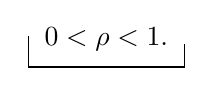
\begin{tikzpicture}
\node[inner sep=0](rho)at(0,0){$0<\rho<1$.};
\draw[line width=.5pt]([xshift=-2mm,yshift=2mm]rho.south west)--([xshift=-2mm,yshift=-2mm]rho.south west)--([xshift=2mm,yshift=-2mm]rho.south east)--([xshift=2mm,yshift=1mm]rho.south east);
\end{tikzpicture}}\end{center}



\begin{center}\GelfandFitDiagram{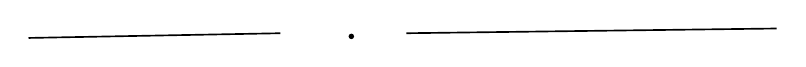
\begin{tikzpicture}[x=1mm,y=1mm]\draw[line width=.6pt](0,0)--(32,.6);\fill(41,.2)circle(.35);\draw[line width=.6pt](48,.6)--(95,1.2);\end{tikzpicture}}\end{center}


\Needspace{7\baselineskip}
\SourcePage{GELFAND-P000368}{26}
\underline{И. М. Гельфанд.}

\begin{GelfandAdjacentEvidence}{GELFAND-P000368}{1}
С ф-ла Радона над конечн. полем.
\Unclear{GELFAND-P000368}{radon-prefix}{Перед «ф-ла» отдельный С-образный знак. Передан «С»; его значение и связь с последующим сокращением не установлены.}
\end{GelfandAdjacentEvidence}

Над $F_q$ $n$-мерн. пр-во. $(x_1,\dots,x_n)$.
\hfill $q^n$ точек.

\begin{GelfandAdjacentEvidence}{GELFAND-P000368}{2}
Изв. интегр. по всем плоскостям.
\begin{equation*}\varphi(p)=\int_{x\in p}f(x)\quad\text{(сумма)}.\end{equation*}
$p$ --- плоскость.



\SourceFigure{GELFAND-P000368}{first-count-caption}{\par\smallskip\centering{\color{black}\GelfandFitDiagram{\begin{minipage}{148mm}\raggedright \GelfandFitDiagram{\begin{tikzpicture}[x=1mm,y=1mm]
\node[anchor=west,inner sep=0](sum)at(0,0){$\displaystyle\sum_{p\ni x_0}\varphi(p)=$};
\node[anchor=west,inner sep=0](count)at([xshift=3mm]sum.east){\small\shortstack{число точек $(n-1)$-мерн.\\проект. пр-ва}};
\node[anchor=west,inner sep=0](factor)at([xshift=5mm]count.east){$f(x_0)$};
\draw[line width=.5pt]([xshift=-1mm,yshift=1mm]count.south west)--([xshift=-1mm,yshift=-2mm]count.south west)--([xshift=1mm,yshift=-2mm]count.south east)--([xshift=1mm,yshift=1mm]count.south east);
\draw[line width=.5pt]([xshift=-1mm,yshift=-1.2mm]count.south west)--([xshift=1mm,yshift=-2.8mm]count.south east);
\draw[line width=.45pt]([xshift=-.5mm,yshift=-5mm]count.south)--([xshift=-.5mm,yshift=-6.5mm]count.south);
\draw[line width=.45pt]([xshift=.5mm,yshift=-5mm]count.south)--([xshift=.5mm,yshift=-6.5mm]count.south);
\node[inner sep=0](alpha)at([yshift=-13mm]count.south){$\displaystyle\frac{q^n-1}{q-1}$};
\draw[line width=.5pt]([xshift=3mm,yshift=-2mm]count.south east)--([xshift=7mm,yshift=-6mm]count.south east);
\draw[line width=.5pt,->]([xshift=11mm,yshift=-2mm]count.south east)--([xshift=11mm,yshift=-7mm]count.south east);
\node[anchor=north,inner sep=0]at([xshift=12mm,yshift=-9mm]count.south east){\small\shortstack{столько раз\\счит. $x_0$}};
\end{tikzpicture}}\end{minipage}}}\par\smallskip }
\end{GelfandAdjacentEvidence}
\begin{GelfandAdjacentEvidence}{GELFAND-P000368}{3}

\begin{equation*}+\frac{q^{n-1}-1}{q-1}\sum_{x\ne x_0}f(x).\end{equation*}



\Unclear{GELFAND-P000368}{cancelled-term-symbol}{В зачёркнутом слагаемом перед $(x_0)$ угловой знак условно передан $A$. $f$ остаётся кандидатом; поперечные штрихи зачёркивания не позволяют установить единственное чтение. Всё слагаемое зачёркнуто; после него знак равенства.\par\smallskip\centering{\color{black}\GelfandFitDiagram{\begin{minipage}{148mm}\raggedright \GelfandFitDiagram{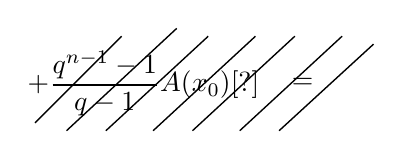
\begin{tikzpicture}[x=1mm,y=1mm]
\node[anchor=west,inner sep=0](old)at(0,0){$\displaystyle+\frac{q^{n-1}-1}{q-1}A(x_0)$[?]};
\draw[line width=.5pt]([xshift=1mm,yshift=-5mm]old.west)--([xshift=12mm,yshift=6mm]old.west);
\draw[line width=.5pt]([xshift=5mm,yshift=-6mm]old.west)--([xshift=19mm,yshift=7mm]old.west);
\draw[line width=.5pt]([xshift=10mm,yshift=-6mm]old.west)--([xshift=23mm,yshift=6mm]old.west);
\draw[line width=.5pt]([xshift=16mm,yshift=-6mm]old.west)--([xshift=29mm,yshift=6mm]old.west);
\draw[line width=.5pt]([xshift=21mm,yshift=-6mm]old.west)--([xshift=34mm,yshift=6mm]old.west);
\draw[line width=.5pt]([xshift=27mm,yshift=-6mm]old.west)--([xshift=40mm,yshift=6mm]old.west);
\draw[line width=.5pt]([xshift=32mm,yshift=-6mm]old.west)--([xshift=44mm,yshift=5mm]old.west);
\node[anchor=west,inner sep=0]at([xshift=4mm]old.east){$=$};
\end{tikzpicture}}\end{minipage}}}\par\smallskip }
\end{GelfandAdjacentEvidence}
\begin{GelfandAdjacentEvidence}{GELFAND-P000368}{4}

\begin{equation*}\sum_x f(x)=\sum_{p\parallel p_0}\varphi(p)\quad\text{\sout{[?]}}\quad\equiv C.\end{equation*}
\Incomplete{GELFAND-P000368}{parallel-condition}{Между суммой по $p\parallel p_0$ и $\equiv C$ зачёркнуты несколько знаков. Их чтение не установлено.}
\end{GelfandAdjacentEvidence}
\begin{GelfandAdjacentEvidence}{GELFAND-P000368}{5}

(не зав. от $p_0$) --- усл. на $\varphi(p)$ --- аналог теор. Пэли-Винера.



\SourceFigure{GELFAND-P000368}{known-sum-caption}{Сумма $\sum_x f(x)$ обведена; под ней подчёркнуто «$C$ --- известно.». Нижний индекс суммы имеет наложенные штрихи и маленькую петлю; $x$ сохранён условно.\par\smallskip\centering{\color{black}\GelfandFitDiagram{\begin{minipage}{148mm}\raggedright \GelfandFitDiagram{\begin{tikzpicture}[x=1mm,y=1mm]
\node[anchor=west,inner sep=0](left)at(0,0){$\displaystyle=\frac{q^n-1}{q-1}f(x_0)+\frac{q^{n-1}-1}{q-1}$};
\node[anchor=west,inner sep=0](total)at([xshift=1mm]left.east){$\displaystyle\sum_x f(x)$};
\node[anchor=west,inner sep=0]at([xshift=3mm]total.east){$\displaystyle-\frac{q^{n-1}-1}{q-1}f(x_0).$};
\draw[line width=.5pt]([xshift=-1mm,yshift=2mm]total.north west)..controls([xshift=2mm,yshift=5mm]total.north east)and([xshift=5mm,yshift=0mm]total.south east)..([xshift=1mm,yshift=-2mm]total.south east)..controls([xshift=-3mm,yshift=-5mm]total.south west)and([xshift=-4mm,yshift=1mm]total.north west)..([xshift=-1mm,yshift=2mm]total.north west);
\node[anchor=north,inner sep=0](known)at([yshift=-8mm]total.south){$C$ --- известно.};
\draw[line width=.5pt]([yshift=-1mm]known.south west)--([yshift=-1mm]known.south east);
\end{tikzpicture}}\end{minipage}}}\par\smallskip }
\end{GelfandAdjacentEvidence}


\uuline{Рота} --- при $q\to1$ получ. перех. к прост. теоремам.
$C_k^n(q)$ --- число $k$-мерных подпр. $n$-мерн. пр-ва.
\begin{equation*}\lim_{q\to1}C_k^n(q)=C_k^n\text{ --- \underline{сочетания}}.\end{equation*}


\Needspace{7\baselineskip}
\SourcePage{GELFAND-P000369}{unlabelled}
\uuline{Кириллов.}

\begin{GelfandAdjacentEvidence}{GELFAND-P000369}{1}
Рассм. произв. обобщ. ф-я $A$ на мн-зии $M$ (напр. $R^n$).
Для неё опр. фронт волны
\begin{equation*}WF(A)\subset T^*M.\end{equation*}
Гладк. ф-я --- нулевой фронт волны (пустой).
Пусть $\xi\in T^*M$.
\begin{gather*}\xi\notin WF(A),\quad\text{если}\\
\langle A,\varphi e^{it\boldsymbol{\psi}}\rangle=o(t^{-n}),\quad\forall n\quad\text{при }t\to+\infty.\end{gather*}
\Unclear{GELFAND-P000369}{phase-reinforced}{Фазовый знак после $it$ сильно утолщён или переписан. Условно передан $\psi$; более ранние штрихи не разделены.}
\end{GelfandAdjacentEvidence}

(при этом $d\psi=\xi$ в точке $\pi_\xi$ и $\varphi\in C_0^\infty$ любая).

Удобно изуч. ф-и, для к-рых фронт волны $\in$ лагр. мн-зия.
\begin{center}\GelfandFitDiagram{\begin{tikzpicture}[x=1mm,y=1mm]
\node[anchor=west,inner sep=0](start)at(0,0){$N\subset M\longrightarrow$};
\node[anchor=west,inner sep=0](normal)at([xshift=3mm]start.east){норм. пучок над $N$};
\draw[line width=.55pt]([yshift=-1mm]normal.south west)--([yshift=-1mm]normal.south east);
\draw[line width=.5pt]([xshift=12mm,yshift=-4mm]normal.south west)--([xshift=12mm,yshift=-7mm]normal.south west);
\node[anchor=north west,inner sep=0]at(0,-14){(перпенд. к $N$ кас. ковекторы).};
\node[anchor=north west,inner sep=0]at(0,-24){Это лагр. подмн. $1/2$-й разм.};
\end{tikzpicture}}\end{center}



\begin{GelfandAdjacentEvidence}{GELFAND-P000369}{2}

\sout{[?]} П. Д. О. --- обобщ. ф-я на $M\times M$ (ядро) с фронтом волны, таким обр. постр. из диагонали.
\Unclear{GELFAND-P000369}{pdo-cancel}{Перед «П. Д. О.» короткое слово густо зачёркнуто. «Напр.» остаётся кандидатом; полное чтение не установлено.}
\end{GelfandAdjacentEvidence}
\begin{GelfandAdjacentEvidence}{GELFAND-P000369}{3}

\begin{center}\GelfandFitDiagram{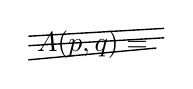
\begin{tikzpicture}
\node[inner sep=0](old)at(0,0){$A(p,q)=$};
\draw[line width=.5pt]([xshift=-1mm,yshift=1mm]old.west)--([xshift=2mm,yshift=2mm]old.east);
\draw[line width=.5pt]([xshift=-1mm,yshift=-.2mm]old.west)--([xshift=2mm,yshift=.8mm]old.east);
\draw[line width=.5pt]([xshift=-1mm,yshift=-2mm]old.west)--([xshift=1mm,yshift=-.5mm]old.east);
\end{tikzpicture}}\end{center}
\begin{equation*}\langle A\mathord{[?]}u\rangle=\int e^{i\psi(x,\xi)}a(x,\xi)u(x)\,dx\,d\xi.\end{equation*}
\Unclear{GELFAND-P000369}{pairing-prefix}{Между $A$ и $u$ усиленный вертикальный знак с верхней петлёй или точкой и нижним загибом; рядом отдельный нижний штрих. $i$, запятая, точка с запятой и зачёркнутый знак остаются возможными чтениями.}
\end{GelfandAdjacentEvidence}

(Знач. $A$ на осн. ф-и $u$).

\begin{GelfandAdjacentEvidence}{GELFAND-P000369}{4}
Всякое $A$ \sout{[?]} с фр. волны, опр. так, зад. этой ф-мой.
\Incomplete{GELFAND-P000369}{lower-cancel}{После «Всякое $A$» отдельный знак густо зачёркнут. Чтение не установлено.}
\end{GelfandAdjacentEvidence}
\begin{GelfandAdjacentEvidence}{GELFAND-P000369}{5}




\Unclear{GELFAND-P000369}{wavefront-prefix}{После «Фр. волны» зачёркнут округлый знак. $\varphi$ передано условно; другое чтение не исключено. Следующее $\in\Lambda$ сохраняется отдельно от зачёркивания.\par\smallskip\centering{\color{black}\GelfandFitDiagram{\begin{minipage}{148mm}\raggedright \begin{equation*}\text{Фр. волны }\text{\sout{$\varphi$}[?]}\in\Lambda=\left\{\underset{\substack{x\in M\\\xi\in T^*M}}{x,\xi}\;\middle|\;d\psi=\xi\,dx\right\}.\end{equation*}\end{minipage}}}\par\smallskip }
\end{GelfandAdjacentEvidence}




\begin{center}\GelfandFitDiagram{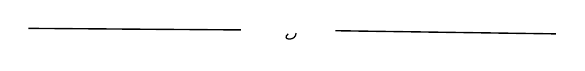
\begin{tikzpicture}[x=1mm,y=1mm]
\draw[line width=.5pt](0,0)--(27,-.2);
\draw[line width=.45pt](33,-.7)..controls(32,-1.5)and(34,-1.7)..(34,-.6);
\draw[line width=.5pt](39,-.3)--(67,-.7);
\end{tikzpicture}}\end{center}


\Needspace{7\baselineskip}
\begin{GelfandAdjacentEvidence}{GELFAND-P000370}{1}
\SourcePage{GELFAND-P000370}{27}
20/$\overline{\underline{\mathrm{IX}}}$ \raisebox{1.5mm}{\rule{.3pt}{1.2mm}}
\Unclear{GELFAND-P000370}{heading-date-tail}{Справа от $20/\mathrm{IX}$ отдельный короткий вертикальный 1-подобный штрих. Его значение не установлено.}
\end{GelfandAdjacentEvidence}
\begin{GelfandAdjacentEvidence}{GELFAND-P000370}{2}




\SourceFigure{GELFAND-P000370}{guest-heading-tab}{\par\smallskip\centering{\color{black}\GelfandFitDiagram{\begin{minipage}{148mm}\raggedright \GelfandFitDiagram{\begin{tikzpicture}[x=1mm,y=1mm]
\node[anchor=west,inner sep=0](guests)at(0,0){\small А. Картан, Картье$^{(?)}$, Кюйпер, Делинь. --- гости.};
\node[inner sep=0](atiyah)at(76,-9){Атья.};
\draw[line width=.55pt](0,-4)--(64,-4)--(64,-13)--(89,-13)--(89,-4)--(132,-4);
\end{tikzpicture}}\end{minipage}}}\par\smallskip }
\end{GelfandAdjacentEvidence}


\begin{GelfandAdjacentEvidence}{GELFAND-P000370}{3}
\underline{И. Бернштейн.} о раб. Godbillon, Vey. Comptes rendus.
$M$ --- комп. мн-зие.
На $M$ зад. форма $\omega$ (\underline{слоение} $S$ коразм. $1$), к-рое интегр.
\begin{equation*}d\omega=\omega\wedge\omega_1.\end{equation*}
--- \sout{[?]}
\Incomplete{GELFAND-P000370}{integrable-cancel}{После формулы старое слово густо зачёркнуто; чтение не установлено.}
\end{GelfandAdjacentEvidence}
\begin{GelfandAdjacentEvidence}{GELFAND-P000370}{4}

\sout{[?]} Ему сопост. $\alpha_s\in H^3(M,R)$, он
\Incomplete{GELFAND-P000370}{class-cancelled-clause}{Перед «Ему сопост.» целая фраза густо зачёркнута; её чтение не установлено.}
\end{GelfandAdjacentEvidence}
\begin{GelfandAdjacentEvidence}{GELFAND-P000370}{5}

\sout{[?]} $=0$, если это расслоение и устойчив при деформ.,
\Incomplete{GELFAND-P000370}{zero-cancel}{После «он» перед $=0$ короткое слово густо зачёркнуто. Уверенное чтение букв не установлено.}
\end{GelfandAdjacentEvidence}
\begin{GelfandAdjacentEvidence}{GELFAND-P000370}{6}

\sout{[?]} $\ne0$.
\Incomplete{GELFAND-P000370}{deformation-cancel}{Между «при деформ.» и $\ne0$ короткое слово перечёркнуто; чтение не установлено.}
\end{GelfandAdjacentEvidence}


\begin{GelfandAdjacentEvidence}{GELFAND-P000370}{7}
Конструкция: сущ. формы $\omega_1$, $\omega_2$:
\begin{gather*}d\omega=\omega\wedge\omega_1;\\d\omega_1=\omega\wedge\omega_2.\end{gather*}
\begin{center}\GelfandFitDiagram{\begin{tikzpicture}
\node[anchor=west,inner sep=0](consider)at(0,0){Рассм.};
\node[anchor=west,inner sep=0](omega)at([xshift=3mm]consider.east){$\Omega=\omega\wedge\omega_1\wedge\omega_2$};
\draw[line width=.5pt]([xshift=-1mm,yshift=1mm]omega.south west)--([xshift=-1mm,yshift=-2mm]omega.south west)--([xshift=1mm,yshift=-2mm]omega.south east)--([xshift=1mm,yshift=1mm]omega.south east);
\end{tikzpicture}}\end{center}
--- замкн. и кл. когом. не зав. от выб. $\omega_1$ и $\omega_2$.
Связь с когомологиями алгебр. есть.




\Unclear{GELFAND-P000370}{quotient-end}{После $SL(2,R)$ усиленный M-подобный знак. $M$ передано условно; чтение наложенных штрихов не установлено.}
\end{GelfandAdjacentEvidence}
\begin{GelfandAdjacentEvidence}{GELFAND-P000370}{8}

\SourceFigure{GELFAND-P000370}{quotient-annotations}{\par\smallskip\centering{\color{black}\GelfandFitDiagram{\begin{minipage}{148mm}\raggedright \GelfandFitDiagram{\begin{tikzpicture}[x=1mm,y=1mm]
\draw[line width=.6pt](0,7)--(0,-59);
\node[anchor=west,inner sep=0]at(5,0){\underline{Пример:}};
\node[anchor=west,inner sep=0]at(35,0){$SL(2,R)\,\boldsymbol M$[?]};
\draw[line width=.75pt](30,5)--(39,-7);
\node[inner sep=0](gamma)at(30,-11){$\Gamma$};
\draw[line width=.5pt](26,-16)..controls(29,-18)and(33,-18)..(35,-16);
\node[anchor=west,inner sep=0]at(22,-23){дискр. подгр.};
\node[anchor=west,inner sep=0]at(76,-12){--- комп.};
\node[anchor=west,inner sep=0]at(8,-38){и $\begin{pmatrix}a&0\\c&b\end{pmatrix}$};
\node[anchor=west,inner sep=0]at(45,-35){плотн. траектории ---};
\node[anchor=west,inner sep=0]at(74,-44){--- всегда.};
\node[anchor=west,inner sep=0]at(22,-56){Тогда он $\ne0$.};
\end{tikzpicture}}\end{minipage}}}\par\smallskip }
\end{GelfandAdjacentEvidence}


Слоение:
\begin{center}\GelfandFitDiagram{\begin{tikzpicture}
\node[anchor=west,inner sep=0](maps)at(0,0){$\begin{gathered}\varphi_i:U_i\longrightarrow R,\\\varphi_j\varphi_i:U_i\cap U_j\longrightarrow R.\end{gathered}$};
\node[anchor=west,inner sep=0](interval)at([xshift=8mm]maps.east){\shortstack{на отрез.\\прямой}};
\draw[line width=.5pt]([xshift=-2mm,yshift=2mm]interval.north west)--([xshift=2mm,yshift=2mm]interval.north east);
\draw[line width=.5pt]([xshift=-2mm,yshift=-2mm]interval.south west)--([xshift=2mm,yshift=-2mm]interval.south east);
\draw[line width=.6pt]([xshift=2mm,yshift=12mm]interval.north east)--([xshift=2mm,yshift=-12mm]interval.south east);
\end{tikzpicture}}\end{center}



Т. к. слои те же, то получ. $\Psi_{ij}:R\to R$ (отрезок).
Если бы $\Psi_{ij}\in$ группе, то коцикл с коэфф. в гр. $\longrightarrow$ пучок и по нему классы когомологий. Но это псевдогруппа.
Но рассм. алгебра Ли, изом. $W_1$ --- форм. вект. поля на прямой, $f(x)\frac{d}{dx}$.
Они $=0$, кроме сущ. $H^3(W_1,R)=R$. Это и есть тот класс.

\begin{GelfandAdjacentEvidence}{GELFAND-P000370}{9}
\uuline{Атья.}
\underline{О спектре самосопр. эллипт. оператора.}
$X$ --- комп. мн-зие,
$D$ --- элл. дифф. опер., самосопр. $D^*=D$.
Дискр. спектр; соб. знач. раздел. на полож. и отр.
Пусть $D=D_t$, $t$ --- парам., спектр мен. вместе с $t$.



\SourceFigure{GELFAND-P000370}{spectrum-sketch}{Наклонённая почти вертикальная линия с двенадцатью различимыми поперечными штрихами разной длины и короткими наложенными штрихами. Один штрих в средней части утолщён. Точные интервалы и разделение всех наложенных штрихов не установлены; числовых меток нет.\par\smallskip\centering{\color{black}\GelfandFitDiagram{\begin{minipage}{68mm}\raggedright \GelfandFitDiagram{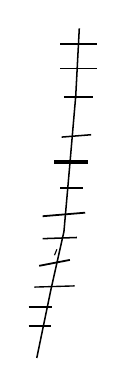
\begin{tikzpicture}[x=.15mm,y=-.15mm]
\draw[line width=.55pt](65,27)--(62,84)--(57,142)--(52,199)--(41,248)--(29,306);
\draw[line width=.55pt](49,40)--(80,40);
\draw[line width=.55pt](49,61)--(80,61);
\draw[line width=.5pt](52,85)--(77,85);
\draw[line width=.55pt](50,119)--(75,117);
\draw[line width=1.35pt](44,140)--(72,140);
\draw[line width=.6pt](49,162)--(68,162);
\draw[line width=.65pt](34,186)--(70,183);
\draw[line width=.55pt](34,205)--(63,204);
\draw[line width=.65pt](31,228)--(57,223);
\draw[line width=.5pt](27,246)--(61,245);
\draw[line width=.55pt](22,263)--(42,263);
\draw[line width=.6pt](22,279)--(41,279);
\draw[line width=.4pt](46,214)--(44,219);
\end{tikzpicture}}\end{minipage}}}\par\smallskip }
\end{GelfandAdjacentEvidence}
\begin{GelfandAdjacentEvidence}{GELFAND-P000370}{10}

Пусть $\underline{D_{t+1}=D_t}$ --- периодичность или



\Unclear{GELFAND-P000370}{unitary-overwrite}{Первый $U$ стоит на основной строке; маленький зачёркнутый старый знак выше и правее него. «на» остаётся кандидатом; точное чтение не установлено. Порядок внесения записей не определён.\par\smallskip\centering{\color{black}\GelfandFitDiagram{\begin{minipage}{148mm}\raggedright \GelfandFitDiagram{\begin{tikzpicture}
\node[anchor=west,inner sep=0](left)at(0,0){$D_{t+1}=$};
\node[anchor=west,inner sep=0](unitary)at([xshift=1mm]left.east){$U$};
\node[anchor=west,inner sep=0](right)at([xshift=2mm]unitary.east){$D_tU^{-1}$};
\node[anchor=south west,inner sep=0](old)at([xshift=.5mm,yshift=2mm]unitary.north east){\scriptsize\sout{[?]}};
\node[anchor=north,inner sep=0]at([yshift=-4mm]right.south){--- общее!};
\end{tikzpicture}}\end{minipage}}}\par\smallskip }
\end{GelfandAdjacentEvidence}

$(U=\mathrm{const})$.


\Needspace{7\baselineskip}
\begin{GelfandAdjacentEvidence}{GELFAND-P000371}{1}
\SourcePage{GELFAND-P000371}{unlabelled}
\begin{equation*}\operatorname{Spec}D_{t+1}=\operatorname{Spec}D_t.\end{equation*}
Спектр двигается (соб. зн. могут сдвигаться на $q$[?]).
\Unclear{GELFAND-P000371}{shift-size}{После «на» усиленный q-подобный знак. $q$ передано условно; вопросительный знак остаётся кандидатом.}
\end{GelfandAdjacentEvidence}
\begin{GelfandAdjacentEvidence}{GELFAND-P000371}{2}

Можно опр. \uuline{целое} число, хар. этот сдвиг.
(Поставить наблюд. в $0$ и смотреть, какая масса прошла влево и вправо.)



\SourceFigure{GELFAND-P000371}{spectrum-graphs}{Верхний рисунок: оси $\lambda,t$, отметки $0,1$, две вертикали и три волнистые кривые. Жирные точки у концов и на оси; нижняя правая точка имеет светлую середину. Ниже шесть различимых наклонных отрезков между почти вертикальными линиями. Точное разделение наложенных штрихов и соединения не установлены.\par\smallskip\centering{\color{black}\GelfandFitDiagram{\begin{minipage}{68mm}\raggedright \GelfandFitDiagram{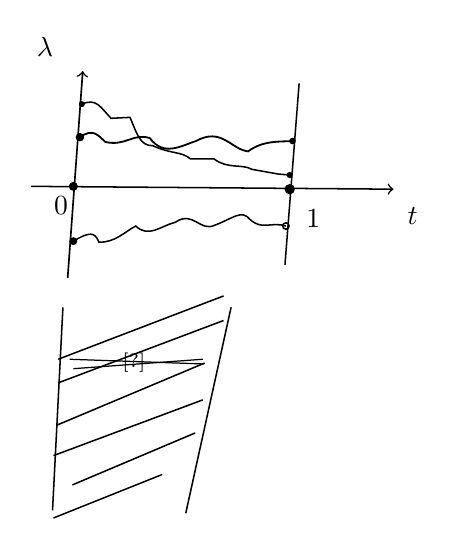
\begin{tikzpicture}[x=.12mm,y=-.12mm]
\draw[line width=.55pt,->](16,182)--(400,185);
\draw[line width=.6pt,->](55,279)--(71,60);
\draw[line width=.55pt](300,73)--(285,265);
\node at(31,34){$\lambda$};\node at(420,213){$t$};\node at(48,202){$0$};\node at(315,216){$1$};
\draw[line width=.55pt](70,95)..controls(86,88)and(90,99)..(101,110)--(121,109)..controls(129,128)and(132,139)..(145,139)..controls(165,148)and(176,145)..(185,153)--(210,153)..controls(224,164)and(240,158)..(250,164)--(278,169)--(290,170);
\draw[line width=.65pt](68,130)..controls(82,120)and(87,128)..(95,135)..controls(116,140)and(125,125)..(142,131)..controls(157,151)and(175,139)..(191,134)..controls(218,119)and(228,143)..(246,145)..controls(262,133)and(280,135)..(293,134);
\draw[line width=.55pt](61,240)..controls(78,230)and(84,230)..(88,241)..controls(105,242)and(117,229)..(127,224)..controls(141,237)and(153,224)..(169,220)..controls(188,207)and(195,231)..(211,223)..controls(230,216)and(239,206)..(248,217)..controls(261,229)and(270,219)..(286,224);
\fill(70,95)circle(3.2);\fill(68,130)circle(4.5);\fill(61,240)circle(4.2);
\fill(290,170)circle(3.3);\fill(293,134)circle(3.5);\draw[line width=.55pt](286,224)circle(3.4);
\fill(61,182)circle(4.8);\fill(290,185)circle(5.5);
\draw[line width=.55pt](50,310)--(39,525);
\draw[line width=.55pt](228,310)--(180,528);
\draw[line width=.55pt](45,365)--(220,298);
\draw[line width=.55pt](45,390)--(220,324);
\draw[line width=.55pt](43,435)--(200,369);
\draw[line width=.55pt](40,467)--(198,408);
\draw[line width=.55pt](60,498)--(190,443);
\draw[line width=.55pt](40,533)--(155,487);
\node[inner sep=0]at(125,369){\scriptsize\sout{[?]}};
\draw[line width=.45pt](57,365)--(199,370);
\draw[line width=.45pt](61,375)--(198,365);
\end{tikzpicture}}\end{minipage}}}\par\smallskip }
\end{GelfandAdjacentEvidence}
\begin{GelfandAdjacentEvidence}{GELFAND-P000371}{3}

\Incomplete{GELFAND-P000371}{graphs-cancelled-caption}{В середине нижнего рисунка зачёркнута короткая надпись, отдельная от наклонных линий. Полного слова или формулы не восстановлено.}
\end{GelfandAdjacentEvidence}


\uuline{Пример.} Спектр. поток $\in Z$.
\begin{equation*}X\text{ --- окр.,}\qquad D_t=-i\frac{d}{dx}+t,\qquad Uf=e^{ix}f.\end{equation*}
\uwave{Поток} $=\pm1$ $(n\to n+1)$.
\uwave{Это топ. инвариант отн. деформ. сем-ва.}
\uuline{Задача:} вычислить спектр. поток через геом. данные задачи: мн-зие, опер., $U$.
Связан с индексом.
Пусть опер. $D$ --- $1$-го пор. (сист.).
Рассм.
\begin{center}\GelfandFitDiagram{\begin{tikzpicture}
\node[anchor=west,inner sep=0](P)at(0,0){$P$};
\node[anchor=west,inner sep=0](op)at(P.east){$\displaystyle\equiv D_t+\frac{\partial}{\partial t}$};
\draw[line width=.55pt]([yshift=1mm]op.south west)--([yshift=-4mm]op.south west)--([xshift=2mm,yshift=-4mm]op.south east)--([xshift=2mm,yshift=2mm]op.south east);
\end{tikzpicture}}\end{center}



\begin{GelfandAdjacentEvidence}{GELFAND-P000371}{4}
на ф-ях $f(x,t)$, $f(x,t+1)=f(x,t)$, $x\in X$, $(U=1)$.
(если $U\ne1$, подправляем $U\otimes1$).
Это \uuline{эллипт.} опер. на $X\times S^1$ (или в рассл., баз. $S^1$ слой $X$).
($D_t$ --- эрм., $\frac{\partial}{\partial t}$ --- косоэрм.).
\underline{Теорема.}



\Unclear{GELFAND-P000371}{theorem-parameter-limits}{Возле правой скобки семейства верхний 1-подобный штрих и нижняя 0-подобная петля соединены с усиленными штрихами скобки. Возможные пределы $1$ и $0$ не отделены уверенно; определённый интервал не приписан.\par\smallskip\centering{\color{black}\GelfandFitDiagram{\begin{minipage}{148mm}\raggedright \GelfandFitDiagram{\begin{tikzpicture}
\node[anchor=west,inner sep=0](family)at(0,0){Спектр. поток $\{D_t\}=$};
\node[anchor=west,inner sep=0](sign)at([xshift=4mm]family.east){$\pm$};
\node[anchor=west,inner sep=0]at([xshift=5mm]sign.east){$\operatorname{index}P$};
\draw[line width=.5pt]([xshift=-4mm,yshift=6mm]sign.center)--([yshift=-5mm]sign.center)--([xshift=7mm,yshift=7mm]sign.center);
\end{tikzpicture}}\end{minipage}}}\par\smallskip }
\end{GelfandAdjacentEvidence}

$=$ ф-ла индекса.



\begin{GelfandAdjacentEvidence}{GELFAND-P000371}{5}
Непоср. док-во сложно. Проще выраз. сп. поток ф-лой.
\uuline{Эвристич. сообр.}
Пусть $D_t$ зав. от $t$ вещ.-аналит. \sout{[?]}
\Incomplete{GELFAND-P000371}{analytic-cancel}{После «вещ.-аналит.» короткое слово полностью перечёркнуто. Чтение не установлено.}
\end{GelfandAdjacentEvidence}
\begin{GelfandAdjacentEvidence}{GELFAND-P000371}{6}

\sout{[?]}
\Unclear{GELFAND-P000371}{branch-cancel}{Слева зачёркнута запись: начальное $t$-подобное начертание и справа $t_0$- или $0$-подобное окончание. $t\ldots t_0$, $t=t_0$, $t=0$, $t\ldots0$ остаются кандидатами; знак отношения не установлен.}
\end{GelfandAdjacentEvidence}
\begin{GelfandAdjacentEvidence}{GELFAND-P000371}{7}

\begin{equation*}\lambda_1(t),\ \lambda_1(t),\ \lambda_2(t),\dots\end{equation*}
--- аналит. ф-и!; опр. для всех $t$.
(Корни хар. полиномов; вещ. $\Rightarrow$ нет ветвлений).



\SourceFigure{GELFAND-P000371}{branch-picture}{Почти вертикальная линия и две группы ветвей на разных уровнях: верхние пересекающиеся кривые, ниже правая восходящая и загнутая вниз ветви и левые наклонные штрихи. Точные соединения густых штрихов и окончания не установлены.\par\smallskip\centering{\color{black}\GelfandFitDiagram{\begin{minipage}{68mm}\raggedright \GelfandFitDiagram{\begin{tikzpicture}[x=.18mm,y=-.18mm]
\draw[line width=.6pt](84,20)--(76,212);
\draw[line width=.55pt](24,62)..controls(49,50)and(64,62)..(78,75)..controls(118,71)and(138,60)..(165,31);
\draw[line width=.65pt](42,95)..controls(56,79)and(70,76)..(81,76)..controls(107,75)and(108,78)..(116,99);
\draw[line width=.55pt](79,122)..controls(107,126)and(128,125)..(142,113);
\draw[line width=.65pt](80,123)..controls(94,130)and(89,153)..(99,167)..controls(104,173)and(113,175)..(120,175);
\draw[line width=.55pt](78,126)..controls(67,151)and(67,169)..(47,194);
\draw[line width=.45pt,dashed](72,126)..controls(58,131)and(54,144)..(47,152);
\end{tikzpicture}}\end{minipage}}}\par\smallskip }
\end{GelfandAdjacentEvidence}



\Needspace{7\baselineskip}
\begin{GelfandAdjacentEvidence}{GELFAND-P000372}{1}
\SourcePage{GELFAND-P000372}{28}
Периодичн. $\Rightarrow$ перестановка их $\sigma$.
\begin{equation*}-i\frac{d}{dx}+t,\qquad\sigma(n)=n+1.\end{equation*}
Эти $\sigma$ --- не произвольные.
\uwave{Орбиты $\sigma$} --- $4$-х классов возм.
1) конечная --- соб. знач., к-рое возвращ.
2) огранич. с одной стороны (из $-\infty$ в $-\infty$ или из $+\infty$ в $+\infty$).
3) неогр. ни с одной стор.



\SourceFigure{GELFAND-P000372}{class-three-scribble}{Справа от случая 3 ломаная нисходящая линия и несколько волнистых или угловых штрихов со сплошными и прерывистыми участками; в середине стрелочный штрих вниз. Точные соединения и геометрическое значение не установлены.\par\smallskip\centering{\color{black}\GelfandFitDiagram{\begin{minipage}{68mm}\raggedright \GelfandFitDiagram{\begin{tikzpicture}[x=.18mm,y=-.18mm]
\draw[line width=.5pt](12,37)--(79,22)..controls(89,19)and(59,48)..(56,49)..controls(63,50)and(80,40)..(81,45)..controls(83,50)and(65,69)..(63,76)--(101,77)..controls(111,84)and(90,102)..(88,104)--(115,105)..controls(122,116)and(102,131)..(101,140)--(125,140)..controls(129,145)and(119,153)..(118,158);
\draw[line width=.45pt,dashed](44,158)--(43,121);
\draw[line width=.55pt](43,121)..controls(46,100)and(61,137)..(69,137);
\draw[line width=.45pt,dashed](69,137)--(75,92);
\draw[line width=.5pt](75,92)--(104,123)..controls(111,132)and(112,122)..(114,118);
\draw[line width=.5pt](104,75)--(137,112);
\draw[line width=.45pt,dashed](137,112)--(143,58);
\draw[line width=.5pt](143,58)--(172,98);
\draw[line width=.45pt,dashed](172,98)--(179,36);
\draw[line width=.5pt](179,36)--(205,73);
\draw[line width=.5pt,->](89,101)--(104,118);
\end{tikzpicture}}\end{minipage}}}\par\smallskip }
\end{GelfandAdjacentEvidence}
\begin{GelfandAdjacentEvidence}{GELFAND-P000372}{2}

\begin{equation*}(|\lambda'(t)|<C|\lambda(t)|.)\end{equation*}
Возрастающие и убывающие --- число орбит об.[?] классов $p$ и $q$ конечно.
\Unclear{GELFAND-P000372}{orbit-class-abbreviation}{Сокращение после «орбит» условно передано «об.». Первая буква имеет разрыв; «сб.» остаётся кандидатом. Сокращение не раскрыто.}
\end{GelfandAdjacentEvidence}
\begin{GelfandAdjacentEvidence}{GELFAND-P000372}{3}

Ф-и $\uuline{\lambda(t)}$ на цилиндре.
3) --- спирали ид. вверх или вниз.



\SourceFigure{GELFAND-P000372}{cylinder-pictures}{Два рисунка между вертикалями: слева перекрывающиеся петли, сплошные и прерывистые участки, сверху стрелка вправо и точка справа ниже. Справа несколько дуг со сплошными и прерывистыми участками. Дополнительные направления и скрытые соединения не установлены.\par\smallskip\centering{\color{black}\GelfandFitDiagram{\begin{minipage}{68mm}\raggedright \GelfandFitDiagram{\begin{tikzpicture}[x=.18mm,y=-.18mm]
\draw[line width=.5pt](15,15)--(25,187);
\draw[line width=.5pt](126,14)--(133,143);
\draw[line width=.5pt](261,16)--(270,182);
\draw[line width=.5pt](355,13)--(368,174);
\draw[line width=.5pt,->](16,29)..controls(57,57)and(82,61)..(119,43);
\draw[line width=.5pt](110,34)..controls(72,42)and(34,47)..(22,78)..controls(15,95)and(62,113)..(101,104)..controls(133,92)and(106,78)..(86,82)..controls(49,87)and(40,112)..(46,130)..controls(61,155)and(111,160)..(128,143);
\draw[line width=.5pt](117,131)..controls(94,113)and(63,132)..(43,159)..controls(29,177)and(39,186)..(62,189);
\draw[line width=.45pt,dashed](62,189)..controls(72,190)and(80,185)..(87,185);
\fill(128,137)circle(2.2);
\draw[line width=.5pt](263,68)..controls(283,91)and(327,64)..(355,22);
\draw[line width=.45pt,dashed](263,68)..controls(289,48)and(324,53)..(362,93);
\draw[line width=.5pt](362,93)..controls(349,120)and(292,155)..(274,134);
\draw[line width=.45pt,dashed](274,134)..controls(285,107)and(342,116)..(365,151);
\draw[line width=.5pt](365,151)..controls(350,174)and(309,184)..(277,185);
\end{tikzpicture}}\end{minipage}}}\par\smallskip }
\end{GelfandAdjacentEvidence}
\begin{GelfandAdjacentEvidence}{GELFAND-P000372}{4}

Число орбит кл. 3) --- конечно. (пересеч. с $\uuline{\text{горизонт.}}$)
\underline{Спектр. поток} $\Rightarrow p-q$. (очев. отсюда).
\underline{Предположение:} пусть соб. вект. не зависят от $t$.
Тогда \sout{[?]} \sout{[?]} точн. реш.
\Incomplete{GELFAND-P000372}{then-cancellations}{После «Тогда» перед «точн. реш.» два коротких слова перечёркнуты. Оба чтения не установлены.}
\end{GelfandAdjacentEvidence}
\begin{GelfandAdjacentEvidence}{GELFAND-P000372}{5}




\Unclear{GELFAND-P000372}{equation-minus}{Первый оператор перед плюсом усилен поверх прежнего знака. $D_t$ передано условно; старые штрихи с возможным $\partial$ не разделены. Под плюсом отдельно $(-)$; эта вставка не заменяет основной плюс.\par\smallskip\centering{\color{black}\GelfandFitDiagram{\begin{minipage}{148mm}\raggedright \GelfandFitDiagram{\begin{tikzpicture}
\node[anchor=west,inner sep=0](open)at(0,0){$\Bigl($};
\node[anchor=west,inner sep=0](D)at(open.east){$\boldsymbol{D_t}$[?]};
\node[anchor=west,inner sep=0](plus)at([xshift=1mm]D.east){$+$};
\node[anchor=west,inner sep=0](partial)at([xshift=1mm]plus.east){$\displaystyle\frac{\partial}{\partial t}\Bigr)$};
\node[anchor=west,inner sep=0](zero)at([xshift=1mm]partial.east){$u=0$};
\node[anchor=north,inner sep=0]at([yshift=-2mm]plus.south){\scriptsize$(-)$};
\node[anchor=west,inner sep=0](caption)at([xshift=5mm,yshift=-1mm]zero.east){запиш. так:};
\draw[line width=.5pt]([xshift=1mm,yshift=5mm]caption.west)..controls([xshift=-3mm,yshift=-3mm]caption.west)and([xshift=1mm,yshift=-1mm]zero.south)..([xshift=1mm,yshift=-6mm]zero.south)..controls([xshift=3mm,yshift=-8mm]zero.south)and([xshift=1mm,yshift=-10mm]zero.south)..([xshift=-1mm,yshift=-11mm]zero.south);
\end{tikzpicture}}\end{minipage}}}\par\smallskip }
\end{GelfandAdjacentEvidence}




\begin{GelfandAdjacentEvidence}{GELFAND-P000372}{6}
\begin{gather*}u_n=C_n\exp\left(-\int\lambda_n(t)\,dt\right),\qquad u=\sum u_n e_n,\quad e_n\text{ --- соб. вектор.}\\
\lambda_n(t+1)=\lambda_{\sigma(n)}(t).\\
\sigma(n)\longrightarrow\infty\quad\Longleftrightarrow\text{конечн. }n\text{ и большие }t.\\
u_n(t)=C_n\exp\left(-\int_0^t\lambda_n(s)\,ds\right).\end{gather*}
$p$ --- число реш. ур-я с $+$,



\SourceFigure{GELFAND-P000372}{q-ditto}{\par\smallskip\centering{\color{black}\GelfandFitDiagram{\begin{minipage}{148mm}\raggedright \GelfandFitDiagram{\begin{tikzpicture}[x=1mm,y=1mm]
\node[inner sep=0]at(0,0){$q$};
\draw[line width=.5pt](5,0)--(31,.3);
\draw[line width=.5pt](34,-.6)--(34.3,.9);
\draw[line width=.5pt](35.5,-.6)--(35.8,.9);
\draw[line width=.5pt,->](39,.4)--(66,.4);
\node[inner sep=0]at(69,.4){$-$};
\node[anchor=west,inner sep=0]at(74,0){, сопр. к ур-ю с $+$.};
\end{tikzpicture}}\end{minipage}}}\par\smallskip }
\end{GelfandAdjacentEvidence}

Конечн. орбиты $\int_0^N\lambda_n(t)\,dt=0$, $N$ --- период.
\begin{center}\GelfandFitDiagram{\begin{tikzpicture}[x=1mm,y=1mm]\draw[line width=.3pt](0,0)--(1,.2);\draw[line width=.3pt](12,-.1)--(13,0);\draw[line width=.3pt](24,.1)--(25,.4);\draw[line width=.3pt](36,.2)--(38,.4);\draw[line width=.3pt](49,.6)--(50,.7);\draw[line width=.3pt](62,.8)--(66,1);\draw[line width=.3pt](80,1)--(83,1.3);\draw[line width=.3pt](98,1.3)--(101,1.6);\end{tikzpicture}}\end{center}
\uwave{Индекс} $=p-q$.
В общ. случае (вектор. движ.) в ур-е $D_t+\frac{\partial}{\partial t}$ вх. доп. член, выраж. движение соб. вект.
Прямое аналит. док-во здесь нельзя.


\Needspace{7\baselineskip}
\begin{GelfandAdjacentEvidence}{GELFAND-P000373}{1}
\SourcePage{GELFAND-P000373}{unlabelled}
\underline{Примеры.}
\textcircled{$1$}. $T:X\longrightarrow X$ --- диффеом.
Опр. расслоение.



\SourceFigure{GELFAND-P000373}{mapping-torus-picture}{\par\smallskip\centering{\color{black}\GelfandFitDiagram{\begin{minipage}{68mm}\raggedright \GelfandFitDiagram{\begin{tikzpicture}[x=.18mm,y=-.18mm]
\draw[line width=.55pt](67,123)..controls(90,99)and(136,87)..(190,103)..controls(217,109)and(224,142)..(196,151)..controls(153,164)and(78,158)..(65,148)..controls(59,140)and(63,128)..(67,123);
\draw[line width=.6pt](68,27)--(66,135);
\draw[line width=.6pt](112,17)--(110,88);
\draw[line width=.55pt](154,19)--(154,101);
\draw[line width=.55pt](194,27)--(195,108);
\node at(31,91){$X$};\node at(164,181){$S^1$};
\end{tikzpicture}}\end{minipage}}}\par\smallskip }
\end{GelfandAdjacentEvidence}
\begin{GelfandAdjacentEvidence}{GELFAND-P000373}{2}

Пусть функториальная ситуация $(X,g,D)$, $g$ --- рим. метрика, $D$ --- самосопр. опер.
(Интересен случай неогр. с $2$-х стор. спектра).
\uwave{Получается тогда:}
\begin{equation*}\underline{X_t,g_t,D_t}.\end{equation*}



\Unclear{GELFAND-P000373}{example-operator-cancel}{После «когда» отдельный зачёркнутый знак; $A$ остаётся кандидатом. Над ним читается «это». Ранее написанный знак не восстановлен уверенно.\par\smallskip\centering{\color{black}\GelfandFitDiagram{\begin{minipage}{148mm}\raggedright \GelfandFitDiagram{\begin{tikzpicture}
\node[anchor=west,inner sep=0](start)at(0,0){(Прим.: $d+\delta$, когда};
\node[anchor=west,inner sep=0](old)at([xshift=3mm]start.east){\sout{[?]}};
\node[anchor=south,inner sep=0]at([yshift=2mm]old.north){это};
\node[anchor=west,inner sep=0]at([xshift=3mm]old.east){самосопр.).};
\end{tikzpicture}}\end{minipage}}}\par\smallskip }
\end{GelfandAdjacentEvidence}

Спектр. поток не зав. от выб. рим. метрики.
Если $T$ --- изометрия, то $D_t=\mathrm{const}$, и сп. поток $=0$.
Инвар. --- препятствие к сущ. метрики, к-рую $T$ сохраняет.
\textcircled{$2$}. $X\times S^1$, опер. $(d+\delta)_t$ на формах.
Скруч. с пом. этого отобр.
Пусть дано
\begin{center}\GelfandFitDiagram{\begin{tikzpicture}
\node[inner sep=0](group)at(0,0){$\pi_1(X)\longrightarrow Z$};
\node[anchor=west,inner sep=0](arrow)at([xshift=2mm]group.east){$\longrightarrow$};
\node[anchor=west,inner sep=0]at([xshift=2mm]arrow.east){$S^1$};
\node[anchor=north,inner sep=0]at([yshift=-2mm]arrow.south){характер.};
\end{tikzpicture}}\end{center}



\begin{GelfandAdjacentEvidence}{GELFAND-P000373}{3}
\begin{equation*}X^{4k+1}\times S^1\end{equation*}
--- инв. Новикова с пом. $L$-полин. Хирцебруха.
\uuline{Делинь в переводе Манина.} О теории мотивов.
Разные теории когомологий алг. мн-зий.
\uuline{25/$\overline{\underline{\mathrm X}}$-71}\quad\rule{.4pt}{4mm}\quad\underline{С. Гельфанд.}
\uuline{Шубертовские клетки.}
Horrocks, Proc. Lond. Math. Soc., $7$, $N^{\circ}$[?] $26$, $1957$.
\Unclear{GELFAND-P000373}{citation}{Между $7$ и $26$ N-подобная запись с коротким верхним или горизонтальным штрихом. $N^{\circ}$ передано условно; $N=$ остаётся кандидатом.}
\end{GelfandAdjacentEvidence}
\begin{GelfandAdjacentEvidence}{GELFAND-P000373}{4}

$G(N,n)$ --- компл. грассм.
\begin{center}\GelfandFitDiagram{\begin{tikzpicture}
\node[anchor=west,inner sep=0](left)at(0,0){($n$-пл. в};
\node[anchor=west,inner sep=0](ambient)at([xshift=2mm]left.east){$C^N$};
\node[anchor=west,inner sep=0]at([xshift=1mm]ambient.east){)};
\draw[line width=.45pt]([xshift=-.6mm,yshift=-2mm]ambient.south)--([xshift=-.6mm,yshift=-3.5mm]ambient.south);
\draw[line width=.45pt]([xshift=.6mm,yshift=-2mm]ambient.south)--([xshift=.6mm,yshift=-3.5mm]ambient.south);
\node[anchor=north,inner sep=0]at([yshift=-5mm]ambient.south){$E$};
\end{tikzpicture}}\end{center}






\SourceFigure{GELFAND-P000373}{schubert-index-caption}{Набор заключён в рамку. Справа линия к «точки, где функц. скачки»; ниже вставлено «разм.», соединённое наклонным штрихом с концом подписи. Точное примыкание этой вставки к нижней строке не установлено.\par\smallskip\centering{\color{black}\GelfandFitDiagram{\begin{minipage}{148mm}\raggedright \GelfandFitDiagram{\begin{tikzpicture}[x=1mm,y=1mm]
\node[anchor=west,inner sep=0](set)at(0,0){$a_1\le a_2\le\dots\le a_n\le N$ --- набор};
\draw[line width=.45pt,rounded corners=1mm]([xshift=-2mm,yshift=2mm]set.north west)rectangle([xshift=2mm,yshift=-2mm]set.south east);
\node[anchor=west,inner sep=0](caption)at([xshift=7mm]set.east){\small\shortstack{--- точки, где\\функц. скачки}};
\node[anchor=north,inner sep=0](dim)at([xshift=3mm,yshift=-4mm]caption.south){\small разм.};
\draw[line width=.45pt]([xshift=2mm]set.east)--([xshift=-1mm]caption.west);
\draw[line width=.45pt]([xshift=-1mm,yshift=-1mm]caption.south east)--(dim.north);
\end{tikzpicture}}\end{minipage}}}\par\smallskip }
\end{GelfandAdjacentEvidence}
\begin{GelfandAdjacentEvidence}{GELFAND-P000373}{5}

Выбран фикс. флаг.
\begin{gather*}E_1\subset E_2\subset\dots\subset E_N=E,\\\dim E_i=i.\\
F\in\Omega(a_1,\dots,a_n),\quad\text{\sout{[?]}}\end{gather*}
\Incomplete{GELFAND-P000373}{schubert-cancel}{После $F\in\Omega(a_1,\dots,a_n)$ целое слово зачёркнуто несколькими жирными горизонтальными штрихами. Его чтение не установлено.}
\end{GelfandAdjacentEvidence}

\begin{gather*}\Updownarrow\\\dim(F\cap E_{a_i+i})=i.\end{gather*}
\begin{equation*}\varphi(i)=\dim(F\cap E_i).\end{equation*}
$\uuline{a_i+i}$ --- точки роста этой ф-и.


\Needspace{7\baselineskip}
\begin{GelfandAdjacentEvidence}{GELFAND-P000374}{1}
\SourcePage{GELFAND-P000374}{29}
Это клеточное разбиение грассм. \underline{мн-зия.}
\uuline{Зад.} Найти все инвар. дифф. формы (кл. Черна).
Связь базиса когом. и колец.
\begin{equation*}(*)\quad U(N)/(U(n)\times U(N-n))=G(N,n)=G/F.\end{equation*}
Форму можно поднять на $U(N)$.
Построение форм:
$de_{ij}$.
$U=(e_{ij})$, $(e_{ij})$ --- матр. эл. ф-я --- на $U(N)$.
\begin{equation*}\theta_{jk}=\sum_{p=1}^N\bar e_{k\boldsymbol p}\,de_{jp},\qquad j=1,\dots,n,\quad k=n+1,\dots,N.\end{equation*}
\Unclear{GELFAND-P000374}{connection-index}{В индексе при $\bar e$ после $k$ сильно усиленный p-подобный знак. $p$ передано условно; $\rho$ остаётся кандидатом.}
\end{GelfandAdjacentEvidence}




\begin{GelfandAdjacentEvidence}{GELFAND-P000374}{2}
$j,k=1,\dots,n$.
\Unclear{GELFAND-P000374}{curvature-factor}{В последнем множителе под чертой округлый знак с горизонтальным штрихом. Условно передан $\Theta$; строчное $\theta$ не исключено. Регистр не установлен из математического согласования.\par\smallskip\centering{\color{black}\GelfandFitDiagram{\begin{minipage}{148mm}\raggedright \GelfandFitDiagram{\begin{tikzpicture}
\node[anchor=west,inner sep=0](theta)at(0,0){$\Theta_{jk}$};
\node[anchor=west,inner sep=0]at([xshift=4mm]theta.east){$\displaystyle=-\frac{1}{2\pi i}\sum_{s=n+1}^N\theta_{js}\wedge\bar{\boldsymbol\Theta}_{ks}$};
\draw[line width=.45pt]([yshift=-3mm]theta.south)--([yshift=-5mm]theta.south);
\node[anchor=north west,inner sep=0]at([yshift=-8mm]theta.south west){форма кривизны расслоения $(*)$.};
\end{tikzpicture}}\end{minipage}}}\par\smallskip }
\end{GelfandAdjacentEvidence}
\begin{GelfandAdjacentEvidence}{GELFAND-P000374}{3}







\SourceFigure{GELFAND-P000374}{omega-caption}{Над $\omega$ «форма на $G$», справа отдельно $G/F$. После «косой» сокращение не установлено полностью: «тенз.» остаётся кандидатом; в строке сохранено начальное т.\par\smallskip\centering{\color{black}\GelfandFitDiagram{\begin{minipage}{148mm}\raggedright \GelfandFitDiagram{\begin{tikzpicture}
\node[anchor=west,inner sep=0](left)at(0,0){Условие того, что};
\node[anchor=west,inner sep=0](omega)at([xshift=2mm]left.east){$\omega$};
\node[anchor=west,inner sep=0](skew)at([xshift=2mm]omega.east){--- косой т[?].};
\node[anchor=south west,inner sep=0]at([xshift=1mm,yshift=4mm]omega.north west){\small --- форма на $G$};
\draw[line width=.4pt]([xshift=1mm,yshift=3mm]omega.north)--([xshift=1mm,yshift=1mm]omega.north);
\node[anchor=west,inner sep=0]at([xshift=9mm]skew.east){$G/F$};
\end{tikzpicture}}\end{minipage}}}\par\smallskip }
\end{GelfandAdjacentEvidence}

1) $\omega(X_1,\dots,X_k)=0$, $X_i\in T(F)$ --- кас. к $F$.
2) $\omega$ --- инв. отн. $F$.
Все $\Theta_{jk}$ удовл. усл. 1).
Отн. $U(N-n)$ инвар., отн. $U(n)$ преобр. сопряжением (присоед. действие).
\begin{center}\GelfandFitDiagram{\begin{tikzpicture}[x=1mm,y=1mm]\draw[line width=.45pt](0,0)--(20,0);\fill(28,-.5)circle(.2);\draw[line width=.45pt](36,-.4)--(72,-1);\end{tikzpicture}}\end{center}
\begin{equation*}GL(n)\ni(x_{ik})_{i,k=1}^n.\end{equation*}
Постр. полиномы от матр. элем., обл. св-вом
\begin{equation*}p(x)=p(gxg^{-1}).\end{equation*}
Коэфф. хар. многочлена --- элем. симм. ф-и.
Надо базис лин. пр-ва.
Пусть $\lambda_1\ge\lambda_2\ge\dots\ge\lambda_n\ge0$, --- целые.
$x$ --- матр., $\alpha_1,\dots,\alpha_n$ --- соб. числа. Надо взять


\Needspace{7\baselineskip}
\begin{GelfandAdjacentEvidence}{GELFAND-P000375}{1}
\SourcePage{GELFAND-P000375}{unlabelled}
{\small симм. ф-и}
\Unclear{GELFAND-P000375}{faint-note-complete}{Мелкая бледная надпись над первым определителем условно передана «симм. ф-и»; «ф-ии» остаётся возможным окончанием.}
\end{GelfandAdjacentEvidence}
\begin{GelfandAdjacentEvidence}{GELFAND-P000375}{2}

\begin{equation*}
\{\lambda\}=
\frac{\begin{vmatrix}
\overset{\text{\sout{[?]}}}{\alpha_1^{\lambda_n}}&\alpha_1^{\lambda_{n-1}+1}&\cdots&\alpha_1^{\lambda_1+n-1}\\
\vdots&\vdots&&\vdots\\
\alpha_n^{\lambda_n}&\alpha_n^{\lambda_{n-1}+1}&\cdots&\alpha_n^{\lambda_1+n-1}
\end{vmatrix}}
{\begin{vmatrix}
1&\alpha_1&\cdots&\alpha_1^{n-1}\\
\vdots&\vdots&&\vdots\\
1&\alpha_n&\cdots&\alpha_n^{n-1}
\end{vmatrix}}
=\{\lambda\}(\chi_{ij})\text{ --- полином.}
\end{equation*}
\Unclear{GELFAND-P000375}{numerator-old-overwrite}{Над первым элементом числителя отдельная густо переписанная запись. Видна $\alpha$-подобная форма и соседние короткие штрихи; прежний индекс не восстановлен уверенно.}
\end{GelfandAdjacentEvidence}
\begin{GelfandAdjacentEvidence}{GELFAND-P000375}{3}

Это характер представл.



\Incomplete{GELFAND-P000375}{cancelled-dimension}{Над зачёркнутым прежним фрагментом обведено «опр. числами». Внизу читается начальное «со» и отдельные конечные штрихи. Слова под густыми горизонталями целиком не установлены.\par\smallskip\centering{\color{black}\GelfandFitDiagram{\begin{minipage}{68mm}\raggedright \GelfandFitDiagram{\begin{tikzpicture}
\node[anchor=west,inner sep=0](old)at(0,0){\sout{со [?]}};
\node[anchor=south west,inner sep=0](insert)at([yshift=5mm]old.north west){опр. числами};
\draw[line width=.45pt]([xshift=-3mm,yshift=-2mm]old.west)--([xshift=-3mm,yshift=2mm]insert.north west)..controls([xshift=12mm,yshift=5mm]insert.north east)and([xshift=7mm,yshift=-1mm]insert.east)..([xshift=2mm,yshift=-2mm]insert.south east)--([xshift=-3mm,yshift=-2mm]old.west);
\end{tikzpicture}}\end{minipage}}}\par\smallskip }
\end{GelfandAdjacentEvidence}
\begin{GelfandAdjacentEvidence}{GELFAND-P000375}{4}

\begin{equation*}\lambda_1\ge\lambda_2\ge\dots\ge\lambda_n\ge0[?].\end{equation*}
\Unclear{GELFAND-P000375}{last-weight-sign}{Последний маленький овал имеет приставной нижний штрих. Условно передано $0$; $a$ остаётся кандидатом.}
\end{GelfandAdjacentEvidence}
\begin{GelfandAdjacentEvidence}{GELFAND-P000375}{5}

\begin{equation*}\{\lambda,\mathord{\text{\tikz[baseline=(circH.base)]\node[draw,circle,inner sep=.4pt](circH){$H$};}}\}=\mathord{\text{\tikz[baseline=(circH.base)]\node[draw,circle,inner sep=.4pt](circH){$H$};}}^{\{\lambda\}}\text{ --- обознач.}\end{equation*}
\Unclear{GELFAND-P000375}{form-power}{Верхняя запись после обведённой буквы содержит $\lambda$ и два фигурных штриха. Условно переданы скобки $\{\lambda\}$; не все наложенные штрихи разделены.}
\end{GelfandAdjacentEvidence}
\begin{GelfandAdjacentEvidence}{GELFAND-P000375}{6}

$\mathord{\text{\tikz[baseline=(circH.base)]\node[draw,circle,inner sep=.4pt](circH){$H$};}}$ --- матр. дифф. форм (они степ. $2$ и коммутируют).
\Unclear{GELFAND-P000375}{circled-form-letter}{В круглой обводке короткая поперечная черта с двумя боковыми штрихами. Условно набрано $H$ в окружности; регистр буквы не установлен. Отдельно сохранены начертания в строке обозначения и в строке определения.}
\end{GelfandAdjacentEvidence}
\begin{GelfandAdjacentEvidence}{GELFAND-P000375}{7}

Положим $a_i=N'-n-\lambda_i$.
\Unclear{GELFAND-P000375}{n-after-weight}{Между $N$ и минусом отдельный тонкий восходящий штрих выше строки. Условно передано $N'$; значение штриха не установлено.}
\end{GelfandAdjacentEvidence}
\begin{GelfandAdjacentEvidence}{GELFAND-P000375}{8}

Тогда



\SourceFigure{GELFAND-P000375}{degree-caption}{\par\smallskip\centering{\color{black}\GelfandFitDiagram{\begin{minipage}{148mm}\raggedright \GelfandFitDiagram{\begin{tikzpicture}
\node[anchor=west,inner sep=0](integral)at(0,0){$\displaystyle\int \mathord{\text{\tikz[baseline=(circH.base)]\node[draw,circle,inner sep=.4pt](circH){$H$};}}^\lambda=1$, а по другим $0$.};
\node[anchor=north,inner sep=0](cycle)at([xshift=6mm,yshift=-5mm]integral.south west){$\Omega(a_1,\dots,a_n)$};
\node[anchor=west,inner sep=0]at([xshift=14mm]cycle.east){\underline{степень} $=$ размерн. шуб. клетки.};
\draw[line width=.5pt]([xshift=3mm,yshift=-3mm]cycle.south east)--([xshift=24mm,yshift=-2mm]cycle.south east);
\fill([xshift=31mm,yshift=-2mm]cycle.south east)circle(.22mm);
\end{tikzpicture}}\end{minipage}}}\par\smallskip }
\end{GelfandAdjacentEvidence}
\begin{GelfandAdjacentEvidence}{GELFAND-P000375}{9}

\underline{Задача} (И. М. Гельфанд)
\begin{equation*}g\in SL(2,F_q).\end{equation*}
Групп. кольцо $\sum_g a(g)g$.
$(a(g)\leftarrow\text{алг. замык. }F_q)$.
\Unclear{GELFAND-P000375}{group-ring-task}{После $a(g)$ отдельный левонаправленный знак с верхним и нижним наклонными штрихами. Передано $\leftarrow$; чтение как принадлежности не принято уверенно.}
\end{GelfandAdjacentEvidence}
\begin{GelfandAdjacentEvidence}{GELFAND-P000375}{10}

Описать его.
\uuline{А. Виноградов.}
Глоб. цель --- изгнать анализ из теории лин. дифф. опер.



\SourceFigure{GELFAND-P000375}{module-production}{\par\smallskip\centering{\color{black}\GelfandFitDiagram{\begin{minipage}{148mm}\raggedright \GelfandFitDiagram{\begin{tikzpicture}
\node[anchor=west,inner sep=0](ring)at(0,0){$K$ --- кольцо,};
\node[anchor=north west,inner sep=0]at([yshift=-2mm]ring.south west){(произв.)};
\node[anchor=west,inner sep=0](modules)at([xshift=22mm]ring.east){$M\longrightarrow N$};
\node[anchor=north west,inner sep=0]at([yshift=-3mm]modules.south west){$2$ модуля над $K$};
\end{tikzpicture}}\end{minipage}}}\par\smallskip }
\end{GelfandAdjacentEvidence}
\begin{GelfandAdjacentEvidence}{GELFAND-P000375}{11}

Классич. ситуация



\SourceFigure{GELFAND-P000375}{classical-caption}{\par\smallskip\centering{\color{black}\GelfandFitDiagram{\begin{minipage}{148mm}\raggedright \GelfandFitDiagram{\begin{tikzpicture}
\node[anchor=west,inner sep=0](ring)at(0,0){$K=C^\infty(L)$};
\node[anchor=north west,inner sep=0]at([xshift=10mm,yshift=-3mm]ring.south west){($L$ --- мн-зие)};
\node[anchor=west,inner sep=0]at([xshift=20mm]ring.east){$C^\infty(E_1)\overset{\mathcal D}{\longrightarrow}C^\infty(E_2)$};
\end{tikzpicture}}\end{minipage}}}\par\smallskip }
\end{GelfandAdjacentEvidence}

$K$ может быть некоммут.


\Needspace{7\baselineskip}
\begin{GelfandAdjacentEvidence}{GELFAND-P000376}{1}
\SourcePage{GELFAND-P000376}{30}
\begin{equation*}M\overset{\mathcal D}{\longrightarrow}N.\end{equation*}
$k\in K$,



\Incomplete{GELFAND-P000376}{cancelled-kd-equality}{Правая часть после $k\mathcal D=$ перечёркнута горизонтальными и наклонными штрихами. Прежние знаки не прочитаны целиком.\par\smallskip\centering{\color{black}\GelfandFitDiagram{\begin{minipage}{148mm}\raggedright \GelfandFitDiagram{\begin{tikzpicture}
\node[anchor=west,inner sep=0](left)at(0,0){$k\mathcal D=$ \sout{[?]}};
\node[anchor=west,inner sep=0]at([yshift=-9mm]left.west){$k^+\mathcal D=\mathcal Dk$.};
\node[anchor=west,inner sep=0](right)at([xshift=24mm]left.east){$(k\mathcal D)f=k(\mathcal Df)$};
\node[anchor=west,inner sep=0]at([yshift=-9mm]right.west){$(k^+\mathcal D)f=\mathcal D(kf)$.};
\end{tikzpicture}}\end{minipage}}}\par\smallskip }
\end{GelfandAdjacentEvidence}




\begin{GelfandAdjacentEvidence}{GELFAND-P000376}{2}
\begin{equation*}\underline{\delta_k=k^+-k}.\end{equation*}
\uuline{Осн. опред.}
Дифф. опер. --- аддит. отобр.



\Incomplete{GELFAND-P000376}{order-overwritten}{После видимого $n$ густо зачёркнут прежний знак. Слева от $n$ фигурные штрихи, ниже «пор.» волнистая линия. Полное старое чтение не установлено.\par\smallskip\centering{\color{black}\GelfandFitDiagram{\begin{minipage}{148mm}\raggedright \GelfandFitDiagram{\begin{tikzpicture}[x=1mm,y=1mm]
\node[anchor=west,inner sep=0](order)at(0,0){пор. $n$ \sout{[?]}};
\draw[line width=.45pt](13,5)..controls(11,4)and(10,2)..(11,1)..controls(12,0)and(12,-1)..(10,-2)..controls(13,-2)and(13,-4)..(12,-5)..controls(14,-5)and(15,-6)..(14,-7);
\draw[line width=.5pt](-2,-5)..controls(2,-3)and(4,-4)..(7,-5)..controls(9,-6)and(11,-4)..(13,-4)..controls(15,-5)and(17,-7)..(19,-6)..controls(21,-4)and(22,-7)..(24,-5);
\node[anchor=west,inner sep=0](D)at(65,8){$\mathcal D:$};
\node[anchor=west,inner sep=0](condition)at(50,-2){$\delta_{k_0}\delta_{k_1}\cdots\delta_{k_n}\mathcal D=0$};
\node[anchor=north west,inner sep=0]at([yshift=-5mm]condition.south west){\uuline{$\forall k_0,\dots,k_n$}};
\end{tikzpicture}}\end{minipage}}}\par\smallskip }
\end{GelfandAdjacentEvidence}
\begin{GelfandAdjacentEvidence}{GELFAND-P000376}{3}

В классич. случае совпад. с обычным.
Так алгебр. стр. теор. гомол. де Рама и т. д. (Спенсер.[?] и пр.)
\Unclear{GELFAND-P000376}{spencer-note}{После «Спенсер» слабые отдельные штрихи перед «и пр.». Точка после фамилии передана условно; вариант без неё не исключён. Сокращение «пр.» не раскрыто.}
\end{GelfandAdjacentEvidence}
\begin{GelfandAdjacentEvidence}{GELFAND-P000376}{4}

$\operatorname{Diff}_n^+(M,N)$ --- все эти операторы.
модуль с умн. \uuline{$k^+$}.



\SourceFigure{GELFAND-P000376}{hom-definition-diagram}{\par\smallskip\centering{\color{black}\GelfandFitDiagram{\begin{minipage}{148mm}\raggedright \GelfandFitDiagram{\begin{tikzpicture}[x=1mm,y=1mm]
\node[anchor=west,inner sep=0](lefttop)at(0,0){$\operatorname{Diff}_n^+(M,N)$};
\draw[line width=.5pt](9,-4)--(9,-10);\draw[line width=.5pt](10.5,-4)--(10.5,-10);
\node[anchor=west,inner sep=0](leftdef)at(14,-7){$def$};
\node[anchor=west,inner sep=0](prefix)at(0,-20){$\operatorname{Hom}_K(M,$};
\node[anchor=west,inner sep=0](target)at([xshift=1mm]prefix.east){$\operatorname{Diff}_n^+N$};
\node[anchor=west,inner sep=0]at([xshift=1mm]target.east){$)$};
\draw[->,line width=.5pt]([xshift=2mm,yshift=-1mm]leftdef.south east)--([xshift=2mm,yshift=3mm]target.north);
\node[anchor=west,inner sep=0](righttop)at(82,0){$\operatorname{Diff}_n(M,N)$};
\draw[line width=.5pt](103,-4)--(103,-10);\draw[line width=.5pt](104.5,-4)--(104.5,-10);
\node[anchor=west,inner sep=0](rightdef)at(108,-7){$def$};
\draw[->,line width=.5pt]([xshift=1mm,yshift=-1mm]rightdef.south)--([xshift=1mm,yshift=-6mm]rightdef.south);
\node[anchor=west,inner sep=0]at(82,-20){$\operatorname{Hom}(J^n(M),N)$};
\end{tikzpicture}}\end{minipage}}}\par\smallskip }
\end{GelfandAdjacentEvidence}
\begin{GelfandAdjacentEvidence}{GELFAND-P000376}{5}




\SourceFigure{GELFAND-P000376}{cojets-caption}{\par\smallskip\centering{\color{black}\GelfandFitDiagram{\begin{minipage}{148mm}\raggedright \GelfandFitDiagram{\begin{tikzpicture}
\node[anchor=west,inner sep=0](definition)at(0,0){$\operatorname{Diff}_n^+(N)=\operatorname{Diff}_n^+(K,N)$};
\node[anchor=west,inner sep=0](arrow)at([xshift=9mm]definition.east){$\Longrightarrow$};
\node[anchor=north,inner sep=0](cojets)at([xshift=-8mm,yshift=-5mm]arrow.south){$\operatorname{Diff}_n^+(N)$};
\node[anchor=north west,inner sep=0](caption)at([xshift=7mm,yshift=-6mm]cojets.south){\uwave{коджеты}.};
\draw[line width=.45pt]([xshift=3mm,yshift=-1mm]cojets.south)--([xshift=-2mm,yshift=1mm]caption.north west);
\end{tikzpicture}}\end{minipage}}}\par\smallskip }
\end{GelfandAdjacentEvidence}
\begin{GelfandAdjacentEvidence}{GELFAND-P000376}{6}

$\Longrightarrow$ теор. сущ. см.
$J^n(K)$ \sout{[?]} --- теор. сущ. тоже есть.
\Incomplete{GELFAND-P000376}{cancelled-after-jets}{После $J^n(K)$ отдельный мелкий знак с наложенными перечёркивающими штрихами. Его целое чтение не восстановлено.}
\end{GelfandAdjacentEvidence}
\begin{GelfandAdjacentEvidence}{GELFAND-P000376}{7}

В $\operatorname{Diff}_nK$ рассм. алг. опер. порожд. $k,k^+$.



\Unclear{GELFAND-P000376}{jet-generators}{Под последним $k$ отдельный нижний N/n-подобный знак. Условно передано $N$; строчное $n$ и чтение без самостоятельного индекса остаются кандидатами. Верхний плюс сохранён отдельно.\par\smallskip\centering{\color{black}\GelfandFitDiagram{\begin{minipage}{68mm}\raggedright \GelfandFitDiagram{\begin{tikzpicture}
\node[anchor=west,inner sep=0](generators)at(0,0){$J^n(K)=\{k,k_{\boldsymbol N}^+\}$};
\draw[line width=.45pt]([xshift=7mm,yshift=4mm]generators.north east)--([xshift=10mm,yshift=7mm]generators.north east);
\draw[line width=.45pt]([xshift=8mm,yshift=3mm]generators.north east)--([xshift=11mm,yshift=6mm]generators.north east);
\end{tikzpicture}}\end{minipage}}}\par\smallskip }
\end{GelfandAdjacentEvidence}






\Needspace{7\baselineskip}
\begin{GelfandAdjacentEvidence}{GELFAND-P000377}{1}
\SourcePage{GELFAND-P000377}{unlabelled}
$D_i$ --- \sout{[?]} функторы $D_i(M)$ (гомологии де Рама).
\Incomplete{GELFAND-P000377}{cancelled-functor-word}{Слово перед «функторы» зачёркнуто несколькими горизонтальными штрихами. Целиком не восстановлено.}
\end{GelfandAdjacentEvidence}
\begin{GelfandAdjacentEvidence}{GELFAND-P000377}{2}

Определим по индукции.
$D=D_1$ --- дифференцирования $K$ в $N$ --- обознач. $D(N)$.
$K\overset{\nabla}{\longrightarrow}N$ дифференцир., если



\Unclear{GELFAND-P000377}{leibniz-argument}{После первого $k$ внутри аргумента один нижний почти вертикальный штрих. Условно передано $k_1k_2$; вариант $k,k_2$ остаётся кандидатом. Отдельная запятая после нижнего $1$ не вставлена.\par\smallskip\centering{\color{black}\GelfandFitDiagram{\begin{minipage}{148mm}\raggedright \GelfandFitDiagram{\begin{tikzpicture}
\node[anchor=west,inner sep=0](leibniz)at(3.5,0){$\nabla(k_1k_2)=k_1\nabla k_2+k_2\nabla k_1$};
\node[anchor=west,inner sep=0]at(0,-1.1){Это д. оп. $1$-го пор.};
\node[anchor=east,inner sep=0]at([yshift=-11mm]leibniz.east){$(-k_1k_2\nabla(1))$.};
\end{tikzpicture}}\end{minipage}}}\par\smallskip }
\end{GelfandAdjacentEvidence}




\begin{GelfandAdjacentEvidence}{GELFAND-P000377}{3}
Это $D(N)$ (вект. поля со зн. в $N$).
$D$ --- обычн. вект. поля.
\begin{equation*}D_2(N)=D\{D(N)\subset\operatorname{Diff}_1^+N\}.\end{equation*}



\SourceFigure{GELFAND-P000377}{inclusion-arrow}{\par\smallskip\centering{\color{black}\GelfandFitDiagram{\begin{minipage}{68mm}\raggedright \GelfandFitDiagram{\begin{tikzpicture}[x=1mm,y=1mm]
\node[anchor=west,inner sep=0]at(0,0){$D$};
\draw[->,line width=.5pt](25,3)..controls(17,5)and(12,0)..(17,-2)..controls(20,-3)and(25,-2)..(29,-2);
\node[anchor=west,inner sep=0]at(36,0){$\operatorname{Diff}_1^{(+)}$};
\end{tikzpicture}}\end{minipage}}}\par\smallskip }
\end{GelfandAdjacentEvidence}
\begin{GelfandAdjacentEvidence}{GELFAND-P000377}{4}




\Unclear{GELFAND-P000377}{module-cancelled}{Старое прилагательное перед «левый» густо зачёркнуто. «правый» передано как кандидат; наложенные штрихи не дают бесспорного целого чтения.\par\smallskip\centering{\color{black}\GelfandFitDiagram{\begin{minipage}{148mm}\raggedright \GelfandFitDiagram{\begin{tikzpicture}
\node[anchor=west,inner sep=0](modulefirst)at(0,0){$D$ --- \sout{правый[?]} \underline{левый} модуль,};
\node[anchor=west,inner sep=0](modulesecond)at(0,-.8){$\operatorname{Diff}_1^+$ --- правый; $D$ --- подмн-во, а не};
\node[anchor=east,inner sep=0](modulelast)at([yshift=-7mm]modulesecond.east){подмодуль};
\draw[line width=.5pt]([xshift=-1mm,yshift=2mm]modulefirst.north west)--([xshift=-3mm,yshift=2mm]modulefirst.north west)--([xshift=-3mm,yshift=-2mm]modulesecond.south west)--([xshift=-1mm,yshift=-2mm]modulesecond.south west);
\draw[line width=.5pt]([xshift=1mm,yshift=3mm]modulelast.east)..controls([xshift=4mm,yshift=2mm]modulelast.east)and([xshift=4mm,yshift=-2mm]modulelast.east)..([xshift=1mm,yshift=-3mm]modulelast.east);
\end{tikzpicture}}\end{minipage}}}\par\smallskip }
\end{GelfandAdjacentEvidence}




\begin{GelfandAdjacentEvidence}{GELFAND-P000377}{5}
В $\operatorname{Diff}_1^{(+)}$ не подмодуль, а влож. --- дифф. опер. $1$-го пор.
$D_2(N)$ --- дифф. $K$ в $\operatorname{Diff}_1^+N$, к-рые уход. в $D(N)$.
\begin{equation*}D_i(N)=D\{D_{i-1}(N)\subset(\operatorname{Diff}_1^+)^{i-1}(N)\}.\end{equation*}
(по индукции).



\SourceFigure{GELFAND-P000377}{date-and-heading}{\par\smallskip\centering{\color{black}\GelfandFitDiagram{\begin{minipage}{148mm}\raggedright \GelfandFitDiagram{\begin{tikzpicture}[baseline=(date.base)]
\node[anchor=west,inner sep=0](date)at(0,0){$1/\overline{\underline{\mathrm{XI}}}\text{-}71$};
\draw[line width=.5pt]([xshift=-2mm,yshift=-2mm]date.south west)--([xshift=1mm,yshift=-2mm]date.south east)--([xshift=1mm,yshift=1mm]date.north east);
\node[anchor=west,inner sep=0]at([xshift=5mm]date.east){\underline{Ур-е Гамильт.-Якоби:}};
\end{tikzpicture}}\end{minipage}}}\par\smallskip }
\end{GelfandAdjacentEvidence}
\begin{GelfandAdjacentEvidence}{GELFAND-P000377}{6}

\begin{equation*}\delta_{k_1}\cdots\delta_{k_1}\mathcal D\quad\text{--- лев. часть ур-я Гам.-Якоби.}\end{equation*}
\Unclear{GELFAND-P000377}{hamilton-repeated-index}{В последнем нижнем индексе густые наложенные штрихи. Условно передано $k_1$; вариант $k_n$ сохранён среди кандидатов.}
\end{GelfandAdjacentEvidence}
\begin{GelfandAdjacentEvidence}{GELFAND-P000377}{7}

(посчитать) ($k_1$ --- всюду одно и то же).
\underline{Теор. сущ. для $J^n(M)$:}
\Unclear{GELFAND-P000377}{jets-theorem-index}{В заголовке $n$; в следующем частном и в $\Pi_s$ стоит $s$. Оба исходных индекса сохранены.}
\end{GelfandAdjacentEvidence}

\begin{equation*}K\otimes_{\mathbb Z}M/\Pi_s=J^s(M).\end{equation*}
$\Pi_s$ --- подмодуль в $K\otimes_{\mathbb Z}M$, порожд. необх. соотн.
\begin{align*}k(k'\otimes m)&=kk'\otimes m,\\
\bar k(k'\otimes m)&=k'\otimes km.
\end{align*}


\Needspace{7\baselineskip}
\begin{GelfandAdjacentEvidence}{GELFAND-P000378}{1}
\SourcePage{GELFAND-P000378}{31}
\begin{equation*}\Delta_{k_0\ldots k_s}=(\bar k_0-k_0)\cdots(\bar k_s-k_s).\end{equation*}
Рассм. подмодуль, порожд. этими $\Delta$.
\begin{equation*}K\otimes_{\mathbb Z}M=\underline A\supset\Delta(A)=\underline{\Pi_s}\quad\text{(обычное опред. джетов).}\end{equation*}
\sout{В простейш[?] случае просто $\operatorname{Diff}_s^{(+)}(K,N[?])$ [?]}
\Incomplete{GELFAND-P000378}{cancelled-upper-line}{Вся строка зачёркнута. Различимы «В простейш[?] случае просто» и формульные штрихи. Окончание прилагательного и последние наложенные знаки не восстановлены целиком.}
\end{GelfandAdjacentEvidence}
\begin{GelfandAdjacentEvidence}{GELFAND-P000378}{2}

\Unclear{GELFAND-P000378}{cancelled-upper-target}{В зачёркнутом $\operatorname{Diff}_s^{(+)}(K,N[?])$ целевой знак N/M-подобный. Условно передано $N$; $M$ остаётся кандидатом.}
\end{GelfandAdjacentEvidence}

\begin{flushright}\underline{$J^s(K)$ проще, чем}\\\underline{в общем случае.}\end{flushright}



\begin{GelfandAdjacentEvidence}{GELFAND-P000378}{3}
$D_1(M)$ --- дифф. опер. без своб. члена.
$D_1(M)=D(M)$ (дифф. $K$ со знач. в $M$).
$D(M)\subset\operatorname{Diff}_1M$.
\begin{equation*}A\in D_1(M)\overset{def}{\Longleftrightarrow}A(k,k_2)=A(k_1)k_2+k_1A(k_2).\end{equation*}
\Unclear{GELFAND-P000378}{derivation-argument}{После первого $k$ в аргументе один нижний изогнутый штрих, условно переданный запятой. Нижний $1$ без отдельной запятой остаётся кандидатом. Дополнительный второй знак не вставлен.}
\end{GelfandAdjacentEvidence}
\begin{GelfandAdjacentEvidence}{GELFAND-P000378}{4}




\SourceFigure{GELFAND-P000378}{margin-module}{\par\smallskip\centering{\color{black}\GelfandFitDiagram{\begin{minipage}{148mm}\raggedright \GelfandFitDiagram{\begin{tikzpicture}[x=1mm,y=1mm]
\node[anchor=west,inner sep=0]at(0,0){$D_0(M)=M$;};
\draw[line width=.5pt](55,6)--(55,-30);
\node[anchor=west,inner sep=0]at(61,0){$D_k(M)$ --- левый};
\node[anchor=west,inner sep=0]at(69,-8){модуль.};
\node[anchor=west,inner sep=0]at(61,-16){(отн. умн. $k$).};
\end{tikzpicture}}\end{minipage}}}\par\smallskip }
\end{GelfandAdjacentEvidence}
\begin{GelfandAdjacentEvidence}{GELFAND-P000378}{5}

\begin{equation*}D_2(M)=D_1(D_1(M)\subset\operatorname{Diff}_1^+(M)).\end{equation*}



\SourceFigure{GELFAND-P000378}{recursive-annotation}{\par\smallskip\centering{\color{black}\GelfandFitDiagram{\begin{minipage}{148mm}\raggedright \GelfandFitDiagram{\begin{tikzpicture}
\node[anchor=west,inner sep=0](recursion)at(0,0){$D_{k+1}(M)=D_1(D_k(M)\subset\operatorname{Diff}^+_{\underbrace{1\,1\ldots1}_{k\text{ раз}}}(M))$};
\node[anchor=north east,inner sep=0](iteration)at([yshift=-7mm]recursion.south east){\shortstack[r]{$k$-кратное применение функтора\\$\operatorname{Diff}_1^+(M)$.}};
\draw[line width=.45pt]([xshift=-37mm,yshift=-2mm]recursion.south east)--([xshift=-38mm,yshift=-5mm]recursion.south east);
\end{tikzpicture}}\end{minipage}}}\par\smallskip }
\end{GelfandAdjacentEvidence}
\begin{GelfandAdjacentEvidence}{GELFAND-P000378}{6}




\Incomplete{GELFAND-P000378}{cancelled-nonmodule}{Над незачёркнутым «не подмодуль» зачёркнута надпись с видимыми частями «не» и «подмод…». Остальные буквы целиком не восстановлены. Выше надписи отдельный короткий вертикальный штрих.\par\smallskip\centering{\color{black}\GelfandFitDiagram{\begin{minipage}{148mm}\raggedright \GelfandFitDiagram{\begin{tikzpicture}[x=1mm,y=1mm]
\node[anchor=west,inner sep=0](nonmodule)at(0,0){$D_1(D_1(M)\subset\operatorname{Diff}^+(M))$.};
\draw[line width=.5pt](22,-5)--(22,-8);
\node[anchor=west,inner sep=0]at(18,-13){\sout{не подмод[?]}};
\node[anchor=west,inner sep=0]at(8,-21){не подмодуль};
\node[anchor=west,inner sep=0]at(8,-29){в структ. $\operatorname{Diff}^+(M)$.};
\end{tikzpicture}}\end{minipage}}}\par\smallskip }
\end{GelfandAdjacentEvidence}
\begin{GelfandAdjacentEvidence}{GELFAND-P000378}{7}




\Incomplete{GELFAND-P000378}{boxed-cancelled-word}{После «Дифф.» перед $K$ густо зачёркнуто слово. Целиком не прочитано.\par\smallskip\centering{\color{black}\GelfandFitDiagram{\begin{minipage}{148mm}\raggedright \GelfandFitDiagram{\begin{tikzpicture}[x=1mm,y=1mm]
\node[anchor=west,inner sep=0]at(4,0){Дифф. \sout{[?]} $K$ в $\operatorname{Diff}_1^+(M)$,};
\node[anchor=west,inner sep=0]at(4,-9){\sout{[?]} у к-рого знач. лежат};
\node[anchor=west,inner sep=0]at(11,-18){в подмн-ве $D_1(M)$.};
\draw[line width=.5pt](0,-23)--(0,0)..controls(0,5)and(2,5)..(8,5)..controls(47,8)and(84,8)..(117,5);
\draw[->,line width=.5pt](1,-23)..controls(35,-23)and(75,-21)..(107,-23);
\end{tikzpicture}}\end{minipage}}}\par\smallskip }
\end{GelfandAdjacentEvidence}
\begin{GelfandAdjacentEvidence}{GELFAND-P000378}{8}

\Incomplete{GELFAND-P000378}{boxed-prefix-complete}{Перед «у» отдельный короткий фрагмент под перечёркивающими штрихами. Целиком не разобран.}
\end{GelfandAdjacentEvidence}
\begin{GelfandAdjacentEvidence}{GELFAND-P000378}{9}







\SourceFigure{GELFAND-P000378}{hatched-strip}{\par\smallskip\centering{\color{black}\GelfandFitDiagram{\begin{minipage}{148mm}\raggedright \GelfandFitDiagram{\begin{tikzpicture}[x=1cm,y=1cm]
\draw(0,0)rectangle(2,1.3);
\draw(0.08,.65)--(.2,1.15);
\draw(.27,.27)--(.9,1.17);
\draw(.68,.19)--(1.45,1.07);
\draw(1.24,.11)--(1.87,.79);
\draw(1.64,.1)--(1.97,.4);
\draw(0,-.13)--(0,.18);\draw(2,-.13)--(2,.18);
\node[below]at(0,-.15){$0$};\node[below]at(2,-.15){$1$};
\node[anchor=west,inner sep=0]at(3,.15){$0=1$ со склеенными концами.};
\node[anchor=west,inner sep=0]at(8.4,-.55){$M$ --- функции.};
\node[anchor=west,inner sep=0]at(8.7,-1.15){\uuline{$M=K$}.};
\end{tikzpicture}}\end{minipage}}}\par\smallskip }
\end{GelfandAdjacentEvidence}
\begin{GelfandAdjacentEvidence}{GELFAND-P000378}{10}

\begin{equation*}D_1(M)=\left\{a\,\text{\sout{[?]}}\dfrac{\partial}{\partial x}+b\dfrac{\partial}{\partial y}\right..\end{equation*}
\Incomplete{GELFAND-P000378}{overwritten-a-argument}{После читаемого $a$ аргумент густо переписан и зачёркнут. Целиком не разобран. Видна открывающая фигурная скобка; закрывающая не добавлена.}
\end{GelfandAdjacentEvidence}
\begin{GelfandAdjacentEvidence}{GELFAND-P000378}{11}

\begin{equation*}\operatorname{Diff}_1^+:a\dfrac{\partial}{\partial x}+b\dfrac{\partial}{\partial y}+c.\end{equation*}
\begin{equation*}K(x)\longrightarrow\text{\sout{[?]}}\,a_k\dfrac{\partial}{\partial x}+b_k\dfrac{\partial}{\partial y}.\end{equation*}
\Incomplete{GELFAND-P000378}{last-field-cutoff}{Сразу после стрелки зачёркнут короткий префикс. Целиком не читается. Строка расположена у нижней границы кадра.}
\end{GelfandAdjacentEvidence}
\begin{GelfandAdjacentEvidence}{GELFAND-P000378}{12}

\Unclear{GELFAND-P000378}{last-field-coefficients}{При $a$ и $b$ компактные k-подобные штрихи. Условно переданы нижние индексы $a_k,b_k$; варианты $a(k),b(k)$ остаются кандидатами. Полные скобки не восстановлены.}
\end{GelfandAdjacentEvidence}



\Needspace{7\baselineskip}
\begin{GelfandAdjacentEvidence}{GELFAND-P000379}{1}
\SourcePage{GELFAND-P000379}{unlabelled}
\begin{align*}
a(k_1k_2)\frac{\partial}{\partial x}+b(k_1k_2)\frac{\partial}{\partial y}
&=a(k_2)\frac{\partial}{\partial x}k_1+b(k_2)\frac{\partial}{\partial x}k_1+\\
&\quad+a(k_1)\frac{\partial}{\partial x}k_2+b(k_1)\frac{\partial}{\partial x}k_2;
\end{align*}
\Unclear{GELFAND-P000379}{repeated-x-denominators}{В четырёх слагаемых справа в знаменателях написано $\partial x$, в том числе при $b$. Эти исходные знаки сохранены.}
\end{GelfandAdjacentEvidence}
\begin{GelfandAdjacentEvidence}{GELFAND-P000379}{2}

Отсюда $a(k_1k_2)=a(k_2)k_1+a(k_1)k_2$ и $b$ --- дифф. и ещё условие:
\begin{align*}
&a(k_2)\frac{\partial k_1}{\partial x}+a(k_1)\frac{\partial k_2}{\partial x}\\
&\quad+b(k_2)\frac{\partial k_1}{\partial x}+b(k_1)\frac{\partial k_2}{\partial x}\quad
\GelfandFitDiagram{\begin{tikzpicture}[baseline=(oldzero.base)]
\node[inner sep=0](oldzero)at(0,0){$=0$};
\draw[line width=.6pt]([xshift=1mm,yshift=-1mm]oldzero.south)--([xshift=2mm,yshift=1mm]oldzero.north);
\end{tikzpicture}}\ldots=0.
\end{align*}
\Unclear{GELFAND-P000379}{condition-cancelled-tail}{После суммы $=0$ перечёркнуто отдельным наклонным штрихом. Далее отдельные точки и слабый нижний штрих; затем незачёркнутое $=0$.}
\end{GelfandAdjacentEvidence}
\begin{GelfandAdjacentEvidence}{GELFAND-P000379}{3}

\begin{equation*}\left(a(k_2)\frac{\partial}{\partial x}+b(k_2)\frac{\partial}{\partial y}\right)k_1+\sim=0.\end{equation*}
\begin{equation*}D_1(k_2)k_1+D_1(k_1)k_2=0.\end{equation*}
\Unclear{GELFAND-P000379}{condition-d-one-index}{Первый нижний $1$ густо переписан. Чтение $D_1$ передано условно; прежние наложенные штрихи целиком не восстановлены.}
\end{GelfandAdjacentEvidence}
\begin{GelfandAdjacentEvidence}{GELFAND-P000379}{4}




\SourceFigure{GELFAND-P000379}{condition-frame}{\par\smallskip\centering{\color{black}\GelfandFitDiagram{\begin{minipage}{148mm}\raggedright \GelfandFitDiagram{\begin{tikzpicture}
\node[anchor=west,inner sep=0]at(0,1.2){$k\longrightarrow D_1(k)$.};
\node[anchor=west,inner sep=0](requirement)at(0,0){$D_1(k_2)k_1+D_1(k_1)k_2=0$.};
\draw[line width=.5pt]([xshift=-3mm,yshift=4mm]requirement.west)--([xshift=-3mm,yshift=-6mm]requirement.west)--([xshift=4mm,yshift=-6mm]requirement.east)..controls([xshift=2mm,yshift=-4mm]requirement.east)and([xshift=2mm,yshift=2mm]requirement.east)..([xshift=2mm,yshift=4mm]requirement.east);
\node[anchor=west,inner sep=0]at([xshift=9mm]requirement.east){--- требование.};
\draw[line width=.5pt](2.5,-1.1)--(4.2,-1.05);\draw[line width=.5pt](5,-1.05)--(7,-1);
\end{tikzpicture}}\end{minipage}}}\par\smallskip }
\end{GelfandAdjacentEvidence}
\begin{GelfandAdjacentEvidence}{GELFAND-P000379}{5}




\Incomplete{GELFAND-P000379}{cancelled-first-mark}{На левом поле перед $D_k(M)$ зачёркнут отдельный знак. Целиком не разобран.\par\smallskip\centering{\color{black}\GelfandFitDiagram{\begin{minipage}{148mm}\raggedright \GelfandFitDiagram{\begin{tikzpicture}
\node[anchor=west,inner sep=0]at(0,0){\sout{[?]}};
\node[anchor=west,inner sep=0](forms)at(1.2,0){\uuline{$D_k(M)$}};
\node[anchor=west,inner sep=0]at([xshift=7mm]forms.east){--- $k$-формы на \sout{[?]} мн-зии со знач. в $M$.};
\node[anchor=west,inner sep=0]at(.4,-1.1){\sout{Опр-е.[?]}};
\node[anchor=west,inner sep=0]at(6.2,-.7){\sout{[?]}};
\end{tikzpicture}}\end{minipage}}}\par\smallskip }
\end{GelfandAdjacentEvidence}
\begin{GelfandAdjacentEvidence}{GELFAND-P000379}{6}

\Incomplete{GELFAND-P000379}{cancelled-manifold-symbol}{Между «на» и «мн-зии» густо зачёркнут знак. Целиком не восстановлен.}
\end{GelfandAdjacentEvidence}
\begin{GelfandAdjacentEvidence}{GELFAND-P000379}{7}

\Unclear{GELFAND-P000379}{cancelled-definition-word}{Под строкой слева зачёркнуто сокращение, условно «Опр-е.»; варианты «Опр-о.» и «Опр.» сохранены. Окончание не раскрыто.}
\end{GelfandAdjacentEvidence}
\begin{GelfandAdjacentEvidence}{GELFAND-P000379}{8}

\Incomplete{GELFAND-P000379}{cancelled-after-k-forms}{Под словом «формы» отдельная зачёркнутая надпись. Целиком не восстановлена.}
\end{GelfandAdjacentEvidence}
\begin{GelfandAdjacentEvidence}{GELFAND-P000379}{9}







\SourceFigure{GELFAND-P000379}{iteration-braces}{\par\smallskip\centering{\color{black}\GelfandFitDiagram{\begin{minipage}{148mm}\raggedright \begin{equation*}
\operatorname{Diff}^+_{\underbrace{1,1,\ldots,1}_{k\text{ раз}}}
=(\operatorname{Diff}_1^+)^k=\underbrace{\operatorname{Diff}_1^+(\cdots\operatorname{Diff}_1^+\cdots}_{k\text{ раз}}).
\end{equation*}\end{minipage}}}\par\smallskip }
\end{GelfandAdjacentEvidence}
\begin{GelfandAdjacentEvidence}{GELFAND-P000379}{10}

\begin{equation*}(\operatorname{Diff}_1^+)^2(M)=\operatorname{Diff}_1(K,\operatorname{Diff}_1^+M).\end{equation*}
\underline{Определение внешних дифф. форм.}
(комплекс де Рама над кольцом $K$)



\SourceFigure{GELFAND-P000379}{definition-arrow}{\par\smallskip\centering{\color{black}\GelfandFitDiagram{\begin{minipage}{148mm}\raggedright \GelfandFitDiagram{\begin{tikzpicture}
\node[anchor=west,inner sep=0](D)at(0,0){$D_i(M)$};
\node[anchor=west,inner sep=0](equal)at([xshift=1mm]D.east){$=$};
\node[anchor=south,inner sep=0](def)at([yshift=1mm]equal.north){$def$};
\node[anchor=west,inner sep=0](hom)at([xshift=1mm]equal.east){$\operatorname{Hom}_K($};
\node[anchor=west,inner sep=0](lambda)at([xshift=1mm]hom.east){$\Lambda_i$};
\node[anchor=west,inner sep=0]at([xshift=1mm]lambda.east){$,M)$;};
\draw[->,line width=.5pt]([xshift=4mm,yshift=1mm]def.east)..controls([xshift=13mm,yshift=7mm]def.east)and([xshift=-1mm,yshift=8mm]lambda.north)..([yshift=1mm]lambda.north);
\end{tikzpicture}}\end{minipage}}}\par\smallskip }
\end{GelfandAdjacentEvidence}
\begin{GelfandAdjacentEvidence}{GELFAND-P000379}{11}

\begin{equation*}\underline{\underline{\Lambda_i=\Lambda_i(\text{\sout{$M$[?]}}\,K)}}.\end{equation*}
\Unclear{GELFAND-P000379}{lambda-argument-correction}{В аргументе перед читаемым $K$ зачёркнут M/N-подобный знак. Условно передано $M$; $N$ остаётся кандидатом.}
\end{GelfandAdjacentEvidence}

\underline{Теорема:} существуют предст. объекты.
$K=\mathbb Z_2$ будет $D_2\ne0$! ($2$-мерн. класс. де Рама).


\Needspace{7\baselineskip}
\begin{GelfandAdjacentEvidence}{GELFAND-P000380}{1}
\SourcePage{GELFAND-P000380}{32}
Рассм. групп. кольцо $\Gamma_2(\mathbb Z_2)$ (с коэфф. из $\mathbb Z_2$).
\Unclear{GELFAND-P000380}{gamma-two-ring}{Первая прописная Г/Γ-подобная, условно передана $\Gamma$. Чтение $F$ остаётся среди кандидатов. Нижние $2$ сохранены.}
\end{GelfandAdjacentEvidence}
\begin{GelfandAdjacentEvidence}{GELFAND-P000380}{2}

Все гр. когом. де Рама --- $\mathbb Z_2$.
Для \uuline{групп. колец} \underline{когом.} де Рама --- \underline{когом.} групп!



\Unclear{GELFAND-P000380}{sequence-j-upper-mark}{У $J$ в последовательности справа сверху отдельный густой знак с наложенными штрихами. Целое чтение и значение не установлены; знак передан как $[?]$.\par\smallskip\centering{\color{black}\GelfandFitDiagram{\begin{minipage}{148mm}\raggedright \GelfandFitDiagram{\begin{tikzpicture}
\node[anchor=west,inner sep=0](zero)at(0,0){$0$};
\node[anchor=west,inner sep=0](J)at(1.4,0){$J^{[?]}$};
\node[anchor=west,inner sep=0](tensor)at(3.3,0){$K\otimes K$};
\node[anchor=west,inner sep=0](ring)at(7.2,0){$K$};
\node[anchor=west,inner sep=0](last)at(9,0){$0$};
\draw[->,line width=.5pt]([xshift=2mm]zero.east)--([xshift=-2mm]J.west);
\draw[->,line width=.5pt]([xshift=2mm]J.east)--([xshift=-2mm]tensor.west);
\draw[->,line width=.5pt]([xshift=2mm]tensor.east)--([xshift=-2mm]ring.west);
\node[anchor=south,inner sep=0]at(5.9,.2){произв.};
\draw[->,line width=.5pt]([xshift=2mm]ring.east)--([xshift=-2mm]last.west);
\node[anchor=west,inner sep=0]at(-.3,.9){$\Lambda_1^{\text{стар}}(K)$};
\end{tikzpicture}}\end{minipage}}}\par\smallskip }
\end{GelfandAdjacentEvidence}




\begin{GelfandAdjacentEvidence}{GELFAND-P000380}{3}
\begin{equation*}J^1/J^2=\Lambda_1,\quad\text{ост. --- внешние степени.}\end{equation*}
\Unclear{GELFAND-P000380}{augmentation-powers}{У числителя справа сверху густые переписанные штрихи. Условно передано $J^1$; варианты $J$ без отдельной степени и $J$ с неустановленной прежней степенью сохранены. Знаменатель $J^2$ читается.}
\end{GelfandAdjacentEvidence}
\begin{GelfandAdjacentEvidence}{GELFAND-P000380}{4}

От поля эти когом. будут $0$, а Виноградовские $\ne0$.
Это опр. неестеств. в категорном смысле.
Они не опр. для \underline{некоммут.} колец.
Это единств. естеств. опред. в категории колец.
\underline{Дифференциал $d$.}



\Incomplete{GELFAND-P000380}{tiny-cancelled-mark}{Под отображением отдельный мелкий знак с наложенными перечёркивающими штрихами. Целиком не восстановлен.\par\smallskip\centering{\color{black}\GelfandFitDiagram{\begin{minipage}{148mm}\raggedright \GelfandFitDiagram{\begin{tikzpicture}
\node[anchor=west,inner sep=0](mapone)at(0,0){$D_k\longrightarrow D_{k-1}(\operatorname{Diff}_1^+)$};
\node[anchor=west,inner sep=0]at([xshift=7mm]mapone.east){\underline{морфизм функторов.}};
\node[anchor=west,inner sep=0]at(0,-.9){(в других терминах $d$).};
\node[anchor=west,inner sep=0](maptwo)at(0,-1.8){т. е. $D_k(M)\longrightarrow D_{k-1}(\operatorname{Diff}_1^+(M))$.};
\node[anchor=west,inner sep=0]at([xshift=7mm]maptwo.east){естеств. отобр.};
\node[anchor=west,inner sep=0]at(4.2,-2.5){\sout{[?]}};
\end{tikzpicture}}\end{minipage}}}\par\smallskip }
\end{GelfandAdjacentEvidence}




\begin{GelfandAdjacentEvidence}{GELFAND-P000380}{5}
\begin{equation*}D_1=D\underset{\text{влож.}}{\longrightarrow}\operatorname{Diff}_1^+\quad(=D_0(\operatorname{Diff}_1^+)).\end{equation*}
\Unclear{GELFAND-P000380}{d-subscript-overwrite}{Первый нижний индекс густо переписан, с петлеобразной частью. Условно передано $1$; $0$ остаётся визуальным кандидатом.}
\end{GelfandAdjacentEvidence}

\begin{equation*}D_1\longrightarrow D_0(\operatorname{Diff}_1^+).\end{equation*}
(не влож. мод., а дифф. опер. $1$-го порядка).
\begin{flushright}$\operatorname{Diff}_n\longrightarrow\operatorname{Diff}_n^+$\\(дифф. опер. порядка $n$).\end{flushright}



\begin{GelfandAdjacentEvidence}{GELFAND-P000380}{6}
Индукция:
\begin{equation*}D_k=D_1\{D_{k-1}\subset(\operatorname{Diff}_1^+)^{k-1}\}.\end{equation*}



\SourceFigure{GELFAND-P000380}{induction-identification}{\par\smallskip\centering{\color{black}\GelfandFitDiagram{\begin{minipage}{148mm}\raggedright \GelfandFitDiagram{\begin{tikzpicture}
\node[anchor=west,inner sep=0]at(0,0){$D_{k-1}(\operatorname{Diff}_1^+)=D_1\{$};
\node[anchor=west,inner sep=0](prefix)at(1,-.9){$D_{k-2}(\operatorname{Diff}_1^+)\subset$};
\node[anchor=west,inner sep=0](target)at([xshift=1mm]prefix.east){$(\operatorname{Diff}_1^+)^{k-2}(\operatorname{Diff}_1^+)$};
\node[anchor=west,inner sep=0]at([xshift=1mm]target.east){$\}$.};
\draw[line width=.45pt]([xshift=-.7mm,yshift=-2mm]target.south)--([xshift=-.7mm,yshift=-4mm]target.south);
\draw[line width=.45pt]([xshift=.7mm,yshift=-2mm]target.south)--([xshift=.7mm,yshift=-4mm]target.south);
\node[anchor=north,inner sep=0]at([yshift=-6mm]target.south){$(\operatorname{Diff}_1)^{k-1}$};
\end{tikzpicture}}\end{minipage}}}\par\smallskip }
\end{GelfandAdjacentEvidence}

Предполож. индукт., что $D_{k-1}\subset D_{k-2}(\operatorname{Diff}_1^+)$, и тогда получим:


\Needspace{7\baselineskip}
\begin{GelfandAdjacentEvidence}{GELFAND-P000381}{1}
\SourcePage{GELFAND-P000381}{unlabelled}
$D_k\subset D_{k-1}(\operatorname{Diff}_1^+)$.
Это \sout{[?]} инъективный морфизм функторов, то есть
\Incomplete{GELFAND-P000381}{cancelled-before-injective}{Перед «инъективный» зачёркнут короткий знак или фрагмент. Целиком не разобран.}
\end{GelfandAdjacentEvidence}
\begin{GelfandAdjacentEvidence}{GELFAND-P000381}{2}




\SourceFigure{GELFAND-P000381}{module-caption}{\par\smallskip\centering{\color{black}\GelfandFitDiagram{\begin{minipage}{148mm}\raggedright \GelfandFitDiagram{\begin{tikzpicture}
\node[anchor=west,inner sep=0](forall)at(0,0){$\forall$ модуля $M$:};
\node[anchor=west,inner sep=0](source)at([xshift=3mm]forall.east){$D_k(M)$};
\node[anchor=west,inner sep=0](subset)at([xshift=1mm]source.east){$\subset$};
\node[anchor=west,inner sep=0]at([xshift=1mm]subset.east){$D_{k-1}(\operatorname{Diff}_1^+(M))$};
\node[anchor=north west,inner sep=0]at([yshift=-2mm]subset.south west){подмодуль};
\end{tikzpicture}}\end{minipage}}}\par\smallskip }
\end{GelfandAdjacentEvidence}
\begin{GelfandAdjacentEvidence}{GELFAND-P000381}{3}

Реализуем на языке дифф. форм:



\Unclear{GELFAND-P000381}{lambda-indices}{В диаграмме нижние $i-1$ слева и $i$ справа написаны поверх усиленных штрихов. Текущая пара передана условно; прежние нижние знаки целиком не восстановлены.\par\smallskip\centering{\color{black}\GelfandFitDiagram{\begin{minipage}{148mm}\raggedright \GelfandFitDiagram{\begin{tikzpicture}
\node[inner sep=0](left)at(4.2,1.7){$\Lambda_{i-1}$};
\node[inner sep=0](right)at(8,1.7){$\Lambda_i$};
\node[inner sep=0](module)at(8,-.2){$M$};
\draw[->,line width=.5pt]([xshift=2mm]left.east)--([xshift=-2mm]right.west);
\node[anchor=south,inner sep=0]at(6.1,1.85){$\nabla$};
\draw[->,line width=.5pt]([yshift=-2mm]right.south)--([yshift=2mm]module.north);
\node[anchor=west,inner sep=0]at(8.2,.8){$h$};
\node[anchor=west,inner sep=0](operator)at(0,0){$\nabla\in\operatorname{Diff}_1^+(\Lambda_{i-1},\Lambda_i)$};
\draw[line width=.5pt]([xshift=-2mm,yshift=3mm]operator.north west)--([xshift=2mm,yshift=3mm]operator.north east)--([xshift=2mm,yshift=-3mm]operator.south east)--([xshift=-4mm,yshift=-3mm]operator.south west);
\end{tikzpicture}}\end{minipage}}}\par\smallskip }
\end{GelfandAdjacentEvidence}




\begin{GelfandAdjacentEvidence}{GELFAND-P000381}{4}
\begin{equation*}D_i(M)=\operatorname{Hom}(\Lambda_i,M).\end{equation*}



\Unclear{GELFAND-P000381}{ordinary-emphasis-mark}{Над «обычные» отдельный толстый почти вертикальный штрих. Отдельная нижняя точка не установлена; полный восклицательный знак не дописан.\par\smallskip\centering{\color{black}\GelfandFitDiagram{\begin{minipage}{148mm}\raggedright \GelfandFitDiagram{\begin{tikzpicture}
\node[anchor=west,inner sep=0]at(0,0){$\Lambda_i=\Lambda_i(K)$.};
\node[anchor=west,inner sep=0]at(5,0){--- универс.};
\node[anchor=west,inner sep=0]at(5.5,-.65){объект.};
\node[anchor=west,inner sep=0]at(5,-1.3){(модуль над $K$).};
\node[anchor=west,inner sep=0]at(1.3,-2.1){\underline{обычные}};
\node[anchor=west,inner sep=0]at(1.1,-2.7){\underline{дифф. формы.}};
\draw[->,line width=.45pt](2,-1.5)..controls(1.8,-1.4)and(1.6,-1.4)..(1.45,-1.55);
\draw[line width=1.1pt](2.3,-1.75)--(2.4,-1.5);
\end{tikzpicture}}\end{minipage}}}\par\smallskip }
\end{GelfandAdjacentEvidence}




\begin{GelfandAdjacentEvidence}{GELFAND-P000381}{5}
\begin{equation*}D_i(M)\overset{\alpha_i}{\longleftrightarrow}D_{i-1}(\operatorname{Diff}_1^+(M)).\end{equation*}
\begin{equation*}h\in\operatorname{Hom}(\Lambda_i,M)\overset{\alpha_i}{\longleftrightarrow}\text{\sout{[?]}}\operatorname{Hom}(\Lambda_{i-1},\operatorname{Diff}_1^+(M)).\end{equation*}
\Incomplete{GELFAND-P000381}{cancelled-hom-prefix}{Перед правым $\operatorname{Hom}$ густо зачёркнут короткий фрагмент. Целиком не восстановлен.}
\end{GelfandAdjacentEvidence}
\begin{GelfandAdjacentEvidence}{GELFAND-P000381}{6}

Пусть зад. дифф. опер. $1$-го пор. $\Lambda_{i-1}\overset{\nabla}{\longrightarrow}\Lambda_i$.
Тогда каждому $h:\Lambda_i\longrightarrow M$ сопост. композиция $h\circ\nabla\in\operatorname{Diff}_1^+(\Lambda_{i-1},M)$.



\SourceFigure{GELFAND-P000381}{alpha-construction}{\par\smallskip\centering{\color{black}\GelfandFitDiagram{\begin{minipage}{148mm}\raggedright \GelfandFitDiagram{\begin{tikzpicture}
\node[anchor=west,inner sep=0](construction)at(0,0){$\forall\nabla\Longrightarrow D_i\overset{\alpha_i(\nabla)}{\longrightarrow}D_{i-1}(\operatorname{Diff}_1^+)$};
\draw[line width=.5pt](2,-.65)..controls(2.7,-.6)and(3.4,-.55)..(4,-.4);
\node[anchor=west,inner sep=0]at(2.2,-1){будет постр.};
\end{tikzpicture}}\end{minipage}}}\par\smallskip }
\end{GelfandAdjacentEvidence}
\begin{GelfandAdjacentEvidence}{GELFAND-P000381}{7}




\SourceFigure{GELFAND-P000381}{composition-identification}{\par\smallskip\centering{\color{black}\GelfandFitDiagram{\begin{minipage}{148mm}\raggedright \GelfandFitDiagram{\begin{tikzpicture}
\node[anchor=west,inner sep=0](first)at(0,0){$h\longrightarrow h\circ\nabla\in\operatorname{Diff}_1^+(\Lambda_{i-1},M)$};
\node[anchor=west,inner sep=0]at([xshift=4mm]first.east){$\Longrightarrow$};
\draw[line width=.5pt](6.4,-.45)--(6.4,-.7);\draw[line width=.5pt](6.55,-.45)--(6.55,-.7);
\node[anchor=west,inner sep=0]at(0,-1.2){$\Longrightarrow$};
\node[anchor=west,inner sep=0](middle)at(4.5,-1.2){$\operatorname{Hom}(\Lambda_{i-1},\operatorname{Diff}_1^+M)$};
\draw[line width=.5pt](8.9,-1.8)--(8.9,-2.2);\draw[line width=.5pt](9.05,-1.8)--(9.05,-2.2);
\draw[line width=.4pt](8.9,-2.05)--(9.05,-2);
\node[anchor=west,inner sep=0]at(4.5,-2.7){$\operatorname{Hom}(J^1\Lambda_{i-1},M)$};
\end{tikzpicture}}\end{minipage}}}\par\smallskip }
\end{GelfandAdjacentEvidence}
\begin{GelfandAdjacentEvidence}{GELFAND-P000381}{8}

И сопр. на $M$



\Incomplete{GELFAND-P000381}{cancelled-arrow-expression}{Первая зачёркнутая надпись лежит под штрихами усиленной стрелки вправо; её целое чтение не восстановлено. Справа отдельно зачёркнуто «дифф.». Обе части и стрелка сохранены.\par\smallskip\centering{\color{black}\GelfandFitDiagram{\begin{minipage}{68mm}\raggedright \GelfandFitDiagram{\begin{tikzpicture}
\node[anchor=west,inner sep=0]at(0,-.08){\sout{[?]}};
\draw[->,line width=1.4pt](0,0)--(2.4,0);
\node[anchor=west,inner sep=0]at(3,0){\sout{дифф.}};
\end{tikzpicture}}\end{minipage}}}\par\smallskip }
\end{GelfandAdjacentEvidence}

гомом. $J^1\Lambda_{i-1}\longrightarrow\Lambda_i$, т. е. дифф. опер. $\Lambda_{i-1}\longrightarrow\Lambda_i$.
Взять $M=\Lambda_i$ и тожд. отобр. даёт то, что надо.


\Needspace{7\baselineskip}
\begin{GelfandAdjacentEvidence}{GELFAND-P000382}{1}
\SourcePage{GELFAND-P000382}{33}
\begin{equation*}\operatorname{Hom}(\Lambda_i,M)\overset{\alpha_i}{\longleftrightarrow}\operatorname{Hom}(\Lambda_{i-1},\operatorname{Diff}_1^+(M)).\end{equation*}
$M=\Lambda_i$ и слева $id$.
Элем. $\operatorname{Hom}(\Lambda_{i-1},\operatorname{Diff}_1^+(M))$ по опр. есть дифф. оператор $1$-го пор. из $\Lambda_{i-1}$ в $M$.
(Находим $\nabla$, к-рый сущ. и единственно).
Надо док., что



\SourceFigure{GELFAND-P000382}{d-square-bracket}{\par\smallskip\centering{\color{black}\GelfandFitDiagram{\begin{minipage}{68mm}\raggedright \GelfandFitDiagram{\begin{tikzpicture}
\node[inner sep=0](square)at(0,0){$d^2=0$.};
\draw[line width=.5pt](-1.1,-.1)--(-1.1,-.5)--(1.1,-.5)--(1.1,-.1);
\end{tikzpicture}}\end{minipage}}}\par\smallskip }
\end{GelfandAdjacentEvidence}
\begin{GelfandAdjacentEvidence}{GELFAND-P000382}{2}

Рассмотрим



\SourceFigure{GELFAND-P000382}{d-square-diagram}{\par\smallskip\centering{\color{black}\GelfandFitDiagram{\begin{minipage}{148mm}\raggedright \GelfandFitDiagram{\begin{tikzpicture}
\node[inner sep=0](first)at(0,0){$D_{i+1}$};
\node[inner sep=0](middle)at(4,0){$D_i(\operatorname{Diff}_1^+)$};
\node[inner sep=0](last)at(9.1,0){$D_{i-1}(\operatorname{Diff}^+_{1,1})$};
\node[inner sep=0](lower)at(9.1,-1.8){$D_{i-1}(\operatorname{Diff}_2^+)$};
\draw[->,line width=.5pt]([xshift=2mm]first.east)--([xshift=-2mm]middle.west);
\draw[->,line width=.8pt]([xshift=2mm]middle.east)--([xshift=-2mm]last.west);
\draw[->,line width=.5pt]([yshift=-3mm]last.south)--([yshift=3mm]lower.north);
\draw[->,line width=.5pt]([xshift=4mm,yshift=-5mm]first.south east)--([xshift=-4mm,yshift=3mm]lower.north west);
\end{tikzpicture}}\end{minipage}}}\par\smallskip }
\end{GelfandAdjacentEvidence}
\begin{GelfandAdjacentEvidence}{GELFAND-P000382}{3}

\underline{В сторону:}
Кольцо $F_2(\mathbb Z_2)$ --- не совпад. с классическими.
$0,1,x$, \sout{[?]}, $1+x$, $(x^2=1)$.
\Incomplete{GELFAND-P000382}{cancelled-group-ring-entry}{После $x$ перед $1+x$ зачёркнут отдельный элемент. Его целое чтение не восстановлено.}
\end{GelfandAdjacentEvidence}
\begin{GelfandAdjacentEvidence}{GELFAND-P000382}{4}

$y=x+1$, тогда $\underline{\underline{y^2=0}}$.
$0,1,y,1+y$, где $\underline{y^2=0}$.
\begin{center}\GelfandFitDiagram{\begin{tikzpicture}
\draw[line width=.5pt](0,0)--(2.3,0);\draw[line width=.5pt](3.2,0)--(6,0);
\end{tikzpicture}}\end{center}
Будет построен опер. Спенсера (граничный).



\SourceFigure{GELFAND-P000382}{spencer-complete-diagram}{Слева сверху $D_{i+1}(\operatorname{Diff}_k^+)$, справа сверху $D_i(\operatorname{Diff}^+_{1,k})$, ниже справа $D_i(\operatorname{Diff}^+_{k+1})$. Горизонтальная стрелка с $\alpha_{i+1}(\operatorname{Diff}_k^+)$; справа стрелка вниз. Короткая диагональная стрелка вправо вниз не доходит до нижнего выражения; на ней перечёркнуто $Spc$. Снизу слева изогнутый указатель к началу верхней горизонтальной. Под диагональной изогнутая вертикальная скобка к «Это гом. Спенсера»; «Спенсера» подчёркнуто. Над правым выражением $\operatorname{Diff}_1(\operatorname{Diff}_k)$ и два коротких наклонных штриха; справа подпись о композиции.\par\smallskip\centering{\color{black}\GelfandFitDiagram{\begin{minipage}{148mm}\raggedright \GelfandFitDiagram{\begin{tikzpicture}
\node[inner sep=0](start)at(1.9,0){$D_{i+1}(\operatorname{Diff}_{k\,\text{\sout{[?]}}}^+)$};
\node[inner sep=0](end)at(8,0){$D_i(\operatorname{Diff}^+_{1,k\,\text{\sout{[?]}}})$};
\node[inner sep=0](down)at(8,-2.2){$D_i(\operatorname{Diff}_{k+1}^+)$};
\draw[->,line width=.5pt]([xshift=2mm]start.east)--([xshift=-2mm]end.west);
\node[anchor=south,inner sep=0]at(5, .2){$\alpha_{i+1}(\operatorname{Diff}_k^+)$};
\node[anchor=west,inner sep=0]at(9.1,1.2){$\operatorname{Diff}_1(\operatorname{Diff}_k)$};
\draw[line width=.45pt](9, .9)--(8.94,.82);\draw[line width=.45pt](9.15,.9)--(9.09,.82);
\draw[->,line width=.5pt]([yshift=-3mm]end.south)--([yshift=3mm]down.north);
\draw[->,line width=.7pt](3.9,-1)--(5.1,-1.9);
\node[inner sep=0]at(4.5,-1.3){$Spc$};
\draw[line width=.65pt](4.2,-1.65)--(4.7,-1.05);
\draw[->,line width=.5pt](2,-1.8)..controls(3,-1.6)and(3.2,-.6)..(4.1,-.18);
\node[anchor=north west,inner sep=0,align=left]at(.8,-1.9){дифф.\\опер. $1$-го пор.};
\draw[line width=.5pt](4.55,-3.3)..controls(4.55,-2.7)and(4.4,-2.1)..(4.75,-1.9);
\node[anchor=north west,inner sep=0]at(4.2,-3.5){Это гом. \underline{Спенсера}};
\node[anchor=north west,inner sep=0,align=left]at(10.2,-1.2){--- гом. модулей\\(композ. дифф.\\опер. даёт\\отобр.};
\node[anchor=north west,inner sep=0]at(10.2,-3.1){$\operatorname{Diff}^+_{1,k}\longrightarrow\operatorname{Diff}_{k+1})$};
\end{tikzpicture}}\end{minipage}}}\par\smallskip }
\end{GelfandAdjacentEvidence}
\begin{GelfandAdjacentEvidence}{GELFAND-P000382}{5}

\Unclear{GELFAND-P000382}{spencer-left-degree}{После $i$ знак с прерывистыми вертикальными частями. Условно $D_{i+1}$; возможно $D_{i-1}$.}
\end{GelfandAdjacentEvidence}
\begin{GelfandAdjacentEvidence}{GELFAND-P000382}{6}

\Unclear{GELFAND-P000382}{spencer-start-cancelled-index}{После левого $k$ зачёркнуты связка и знак, похожий на $2$. Возможны старые $-2$, $+2$ или иной индекс с конечной $2$.}
\end{GelfandAdjacentEvidence}
\begin{GelfandAdjacentEvidence}{GELFAND-P000382}{7}

\Incomplete{GELFAND-P000382}{spencer-end-cancelled-index}{После правого $k$ дополнительный индексный фрагмент зачёркнут. Его целое чтение не восстановлено.}
\end{GelfandAdjacentEvidence}
\begin{GelfandAdjacentEvidence}{GELFAND-P000382}{8}

\underline{Комплекс Спенсера:}



\SourceFigure{GELFAND-P000382}{spencer-chain}{\par\smallskip\centering{\color{black}\GelfandFitDiagram{\begin{minipage}{148mm}\raggedright \begin{equation*}
M\overset{\Delta}{\longleftarrow}\operatorname{Diff}_k^+M\overset{Spc}{\longleftarrow}D(\operatorname{Diff}_{k-1}^+M)\overset{Spc}{\longleftarrow}\cdots\overset{Spc}{\longleftarrow}\text{\sout{$D_i$}}
\end{equation*}\end{minipage}}}\par\smallskip }
\end{GelfandAdjacentEvidence}
\begin{GelfandAdjacentEvidence}{GELFAND-P000382}{9}

\Unclear{GELFAND-P000382}{spencer-cancelled-endpoint}{Крайнее зачёркнутое выражение условно $D_i$; нижний крючок допускает $D_1$.}
\end{GelfandAdjacentEvidence}
\begin{GelfandAdjacentEvidence}{GELFAND-P000382}{10}

\Unclear{GELFAND-P000382}{spencer-label-endings}{У всех четырёх подписей третий знак похож на $c/e$ или нижний $e$-подобный знак. Условно $Spc$; возможно $Spe$. Диагональная подпись перечёркнута; три нижние текущие.}
\end{GelfandAdjacentEvidence}



\Needspace{7\baselineskip}
\begin{GelfandAdjacentEvidence}{GELFAND-P000383}{1}
\SourcePage{GELFAND-P000383}{unlabelled}
\begin{equation*}\longleftarrow D_i(\operatorname{Diff}_{k-i}^+M)\longleftarrow\cdots\end{equation*}
Это резольв. Спенсера (корезольв. См.)
\Unclear{GELFAND-P000383}{resolvent-parenthesis}{В скобках «корезольв. См.»; последние две соединённые буквы допускают «См.» или «Сп.». Сокращение оставлено нераскрытым.}
\end{GelfandAdjacentEvidence}
\begin{GelfandAdjacentEvidence}{GELFAND-P000383}{2}




\Unclear{GELFAND-P000383}{small-jets-note}{Мелкое слово условно «там»; возможно «тан» или «точ». Затем «для $J$». Над областью «для» отдельный короткий вертикальный штрих.\par\smallskip\centering{\color{black}\GelfandFitDiagram{\begin{minipage}{68mm}\raggedright \GelfandFitDiagram{\begin{tikzpicture}
\node[inner sep=0]at(0,0){\small там для $J$.};
\draw[line width=.5pt](-.1,.35)--(-.1,.55);
\end{tikzpicture}}\end{minipage}}}\par\smallskip }
\end{GelfandAdjacentEvidence}
\begin{GelfandAdjacentEvidence}{GELFAND-P000383}{3}

\begin{gather*}
M\longleftarrow\operatorname{Diff}_{\infty}^+\{M\}\longleftarrow D_1(\operatorname{Diff}_{\infty}^+\{M)\\
\longleftarrow\cdots\longleftarrow D_i(\operatorname{Diff}_{\infty}^+M)\longleftarrow\cdots
\end{gather*}
\Unclear{GELFAND-P000383}{resolvent-chain}{При первом $M$ скобки фигурные, с усиленными штрихами. При втором $M$ слева фигурная-подобная скобка, справа круглая закрывающая. Условно передано $D_1(\operatorname{Diff}_{\infty}^+\{M)$; старая форма усиленных штрихов целиком не установлена. Все стрелки влево.}
\end{GelfandAdjacentEvidence}
\begin{GelfandAdjacentEvidence}{GELFAND-P000383}{4}

\begin{equation*}\operatorname{Diff}_{\infty}^+M=\underset{\longrightarrow}{\lim}\operatorname{Diff}_i^+.\end{equation*}



\SourceFigure{GELFAND-P000383}{limit-embedding}{\par\smallskip\centering{\color{black}\GelfandFitDiagram{\begin{minipage}{148mm}\raggedright \GelfandFitDiagram{\begin{tikzpicture}
\node[inner sep=0]at(0,0){$(\operatorname{Diff}_i^+$};
\node[inner sep=0]at(4.2,0){$\operatorname{Diff}_{i+1}^+)$};
\draw[->,line width=.5pt](2.1,.3)..controls(1.1,.3)and(1.1,-.35)..(2.25,-.35);
\end{tikzpicture}}\end{minipage}}}\par\smallskip }
\end{GelfandAdjacentEvidence}
\begin{GelfandAdjacentEvidence}{GELFAND-P000383}{5}

\underline{Это} \underline{комплекс}.
И отобр. (пока не опред.)
\begin{equation*}\operatorname{Diff}_k^+M\longrightarrow M.\end{equation*}
\begin{equation*}\operatorname{Diff}_s^+(M,N)\overset{def}{=}\operatorname{Hom}_K(M,\operatorname{Diff}_s^+N).\end{equation*}
Пусть $\operatorname{Diff}^+N\overset{\Delta}{\longrightarrow}N$; $\Delta$ --- опер. порядка $s$.
Тогда по гом. $h:\underline{\underline{M\longrightarrow\operatorname{Diff}^+N}}$ стр. композиция.
(надо взять в кач. $M$ $\operatorname{Diff}_s^+N$ и тожд. отобр.
\begin{center}\GelfandFitDiagram{\begin{tikzpicture}
\node[anchor=west,inner sep=0]at(0,0){$id\in\operatorname{Hom}(M,\operatorname{Diff}_s^+N)$.};
\draw[line width=.2pt](3.5,-.25)--(4.05,-.75);
\node[anchor=west,inner sep=0]at(0,-1.15){получ. $\operatorname{Diff}_s^+N\longrightarrow N$.};
\end{tikzpicture}}\end{center}
Это опред. $1$-го морфизма.
\SourceFigure{GELFAND-P000383}{universal-composition}{Отображение $M\longrightarrow\operatorname{Diff}^+N$ при $h$ дважды подчёркнуто. Ниже $\operatorname{Hom}$ тонкий отдельный диагональный штрих вправо вниз, без наконечника, к области начала следующей стрелки. Перед «надо» открывающая круглая скобка; отдельная общая закрывающая после нижнего $N$ не видна.}
\end{GelfandAdjacentEvidence}

\begin{equation*}\Delta\in\operatorname{Diff}_s^+(K,M)\longrightarrow\underline{\underline{\Delta(1)}}.\end{equation*}



\underline{Заголовки}:
Все резольв. Спенсера не в коорд. форме (отличие от Спенсера).
Индекс над любым кольцом.
Гамильтонов формализм для $\forall$ кольца.
След. раз --- \underline{\underline{продолжение}}.





\Needspace{7\baselineskip}
\SourcePage{GELFAND-P000384}{34}



\begin{GelfandAdjacentEvidence}{GELFAND-P000384}{1}
$[\;]$
\SourceFigure{GELFAND-P000384}{date-margin}{\par\smallskip\centering{\color{black}\GelfandFitDiagram{\begin{minipage}{68mm}\raggedright \GelfandFitDiagram{\begin{tikzpicture}
\node[inner sep=0]at(0,0){$8$};\node[inner sep=0]at(.5,0){$\mathrm{XI}$};
\draw[line width=.5pt](.2,-.24)--(.3,.28);\draw[line width=.5pt](.32,.3)--(.8,.3)--(.8,-.23)--(.27,-.23);
\draw[line width=.5pt](-.12,-.4)--(.75,-.4);
\node[anchor=west,inner sep=0]at(1.2,0){\underline{Лемма 1}.};
\end{tikzpicture}}\end{minipage}}}\par\smallskip }
\end{GelfandAdjacentEvidence}
\begin{GelfandAdjacentEvidence}{GELFAND-P000384}{2}

$\operatorname{Diff}_n^+(M,N)$ при фиксир. $N$ --- функтор от $M$ (контравар.).



\SourceFigure{GELFAND-P000384}{module-functor}{\par\smallskip\centering{\color{black}\GelfandFitDiagram{\begin{minipage}{68mm}\raggedright \GelfandFitDiagram{\begin{tikzpicture}
\node[draw,ellipse,inner xsep=3mm,inner ysep=2mm](a)at(0,0){мод.};
\node[draw,ellipse,inner xsep=3mm,inner ysep=2mm](b)at(4,0){мод.};
\draw[->,line width=.5pt]([xshift=3mm]a.east)--([xshift=-3mm]b.west);
\end{tikzpicture}}\end{minipage}}}\par\smallskip }
\end{GelfandAdjacentEvidence}
\begin{GelfandAdjacentEvidence}{GELFAND-P000384}{3}

(а если брать $\operatorname{Diff}_n(M,N)$, то это функтор от $N$ при фикс. $M$ (ковар.)).
\underline{Док-во}: $\mathcal F^+_{N,n}(M)=\operatorname{Diff}_n^+(M,N)$.
Если $f:M_1\longrightarrow M_2$ гом. мод. $\Longrightarrow$
\begin{equation*}\mathcal F^+_{N,n}(f):\operatorname{Diff}_n^+(M_2,N)\longrightarrow\operatorname{Diff}_n^+(M_1,N).\end{equation*}



\Unclear{GELFAND-P000384}{variance-proof-inset}{В правой вставке написано $D\circ f:M_1\longrightarrow M_2$; последнее $M_2$ сохранено. Рамка открыта сверху, с нижним длинным штрихом и короткими боковыми загибами.\par\smallskip\centering{\color{black}\GelfandFitDiagram{\begin{minipage}{148mm}\raggedright \GelfandFitDiagram{\begin{tikzpicture}
\node[inner sep=0](inset)at(0,0){$D:M_2\longrightarrow N\leadsto D\circ f:M_1\longrightarrow M_2$};
\draw[line width=.5pt]([xshift=-7mm,yshift=3mm]inset.north west)--([xshift=-2mm,yshift=3mm]inset.north west)--([xshift=-2mm,yshift=-2mm]inset.south west)--([xshift=2mm,yshift=-2mm]inset.south east)--([xshift=2mm,yshift=1mm]inset.east)--([xshift=4mm,yshift=1mm]inset.east);
\end{tikzpicture}}\end{minipage}}}\par\smallskip }
\end{GelfandAdjacentEvidence}
\begin{GelfandAdjacentEvidence}{GELFAND-P000384}{4}

И это есть гомоморфизм модулей, т. к.



\Incomplete{GELFAND-P000384}{derivative-cancel-complete}{Перед $D(kf)$ отдельный короткий густо зачёркнутый фрагмент. Его целое чтение не восстановлено.\par\smallskip\centering{\color{black}\GelfandFitDiagram{\begin{minipage}{148mm}\raggedright \GelfandFitDiagram{\begin{tikzpicture}
\node[anchor=west,inner sep=0](prefix)at(0,0){\sout{[?]}};
\node[anchor=west,inner sep=0](before)at(.7,0){$D(kf)=(Dk)f=$};
\node[anchor=west,inner sep=0](action)at(before.east){$(k^+D)$};
\node[anchor=west,inner sep=0](post)at(action.east){$f$};
\node[anchor=west,inner sep=0](reorder)at(post.east){$=Dfk$};
\node[anchor=west,inner sep=0]at(reorder.east){$=k^+(Df)$};
\draw[line width=.5pt]([xshift=2mm,yshift=-2mm]action.south west)..controls([yshift=-3mm]action.south)and([yshift=-3mm]action.south)..([xshift=-2mm,yshift=-2mm]action.south east);
\draw[line width=.5pt]([yshift=-2mm]post.south)--([xshift=-.2mm,yshift=-3mm]post.south);
\draw[line width=.5pt]([xshift=2mm,yshift=-2mm]reorder.south west)--([yshift=-2mm]reorder.south east);
\end{tikzpicture}}\end{minipage}}}\par\smallskip }
\end{GelfandAdjacentEvidence}

\begin{equation*}\Longrightarrow(k^+D)f=k^+(Df).\end{equation*}



\begin{GelfandAdjacentEvidence}{GELFAND-P000384}{5}
Аналогично, если рассм. $\operatorname{Diff}_n(M,N)$ как функтор от $N$, то $f$ надо послать слева и это тоже получ. гомом. модулей.
$[\;]$ \underline{Лемма 2}. Пусть $A\in\operatorname{Diff}_1(K,M)$. Тогда
\begin{equation*}A(k_1k_2)=k_1A(k_2)+k_2A(k_1)-k_1k_2A(1).\qquad(1)\end{equation*}
и наоборот, если $A:K\longrightarrow M$ --- аддит. отобр., удовл. $(1)$, то $A\in\operatorname{Diff}_1(K,M)$.
\underline{Док-во}: Общая ситуация $A\in\operatorname{Diff}_1(N,M)\Longleftrightarrow$
\begin{equation*}Ak_0k_1=k_0Ak_1+k_1Ak_0-k_0k_1A\quad(\forall k_0,k_1).\qquad(2)\end{equation*}
Для $N=K$ это значит, что
\begin{equation*}A(k_0k_1k)=k_0A(k_1k)+k_1A(k_0k)-k_0k_1A(k).\qquad(3)\end{equation*}
Полагая $k=1$, получим $(1)$. Обратно пусть $(1)$ вып.
\Unclear{GELFAND-P000384}{tiny-proof-word}{После «пусть $(1)$» мелкое «вып.»; возможно «выч.». Сокращение не раскрыто.}
\end{GelfandAdjacentEvidence}
\begin{GelfandAdjacentEvidence}{GELFAND-P000384}{6}




\Unclear{GELFAND-P000384}{proof-reference-three}{Номер $3$ густо усилен поверх прежнего штриха; возможна переписанная $2$. Слева две близкие открывающие скобки, справа одна закрывающая. Выше мелкая вставка $(\forall k_0,k_1,k)$.\par\smallskip\centering{\color{black}\GelfandFitDiagram{\begin{minipage}{68mm}\raggedright \GelfandFitDiagram{\begin{tikzpicture}
\node[inner sep=0]at(2.6,.45){\small$(\forall k_0,k_1,k)$};
\node[anchor=west,inner sep=0]at(0,0){Док-м $((3)$.};
\end{tikzpicture}}\end{minipage}}}\par\smallskip }
\end{GelfandAdjacentEvidence}
\begin{GelfandAdjacentEvidence}{GELFAND-P000384}{7}



\Unclear{GELFAND-P000384}{middle-cancel-complete}{Перечёркнуто всё $k_1kk_0A(1)$; последний аргумент усилен и допускает $A(k)$. Отдельно перечёркнут заключительный член $-k_0k_1kA(1)$.\par\smallskip\centering{\color{black}\GelfandFitDiagram{\begin{minipage}{148mm}\raggedright 
\begin{center}\GelfandFitDiagram{\begin{tikzpicture}
\node[anchor=west,inner sep=0](proofbefore)at(0,0){\small$A(k_0k_1k)=A(k_0(k_1k))=k_0A(k_1k)+$};
\node[anchor=west,inner sep=0](substitute)at(proofbefore.east){\small$k_1(kA(k_0))$};
\node[anchor=west,inner sep=0]at(substitute.east){\small$-k_0k_1kA(1)=$};
\draw[line width=.5pt]([yshift=-2mm]substitute.south west)--([yshift=-3mm]substitute.south west)--([yshift=-3mm]substitute.south east)--([yshift=-2mm]substitute.south east);
\draw[line width=.4pt]([yshift=-3mm]substitute.south)--([yshift=-6mm]substitute.south);
\end{tikzpicture}}\end{center}
\begin{equation*}\bigl(kA(k_0)=A(kk_0)+kk_0A(1)-k_0A(k)\bigr)\end{equation*}
\begin{center}\GelfandFitDiagram{\begin{tikzpicture}
\node[anchor=west,inner sep=0](expandedfirst)at(0,0){\small$=k_0A(k_1k)+$};
\node[anchor=west,inner sep=0](expandedmiddle)at(expandedfirst.east){\small$k_1A(k_0k)+\text{\sout{$k_1kk_0A(1)$}}-k_1k_0A(k)$};
\node[anchor=west,inner sep=0]at(expandedmiddle.east){\small$-\text{\sout{$k_0k_1kA(1)$}}.$};
\draw[line width=.5pt]([yshift=-2mm]expandedmiddle.south west)--([yshift=-3mm]expandedmiddle.south west)--([yshift=-3mm]expandedmiddle.south east)--([yshift=-2mm]expandedmiddle.south east);
\end{tikzpicture}}\end{center}\end{minipage}}}\par\smallskip }
\end{GelfandAdjacentEvidence}

\begin{equation*}=k_0Ak_1k+k_1Ak_0k-k_0k_1Ak,\end{equation*}
что и требовалось.



\begin{GelfandAdjacentEvidence}{GELFAND-P000384}{8}
\underline{Следствие}: $A\in\operatorname{Diff}_1(K,M)\Longrightarrow A-A(1)$ --- дифференцирование $K$ в $M$.
\underline{Лемма 3}. Пусть $A_1\in\operatorname{Diff}_m(M_1,M_2)$, $B\in\operatorname{Diff}_n(M_2,M_3)$.
\Unclear{GELFAND-P000384}{lemma-three-first-index}{В гипотезе под первым $A$ дополнительный усиленный $1$-подобный индекс. Условно $A_1$; прежний нижний знак не установлен.}
\end{GelfandAdjacentEvidence}

Тогда $B\circ A\in\operatorname{Diff}_{m+n}(M_1,M_3)$.
\underline{Док-во}: индукция по $\underline{m+n}$.
При $m+n=0$ $(m=n=0)$ всё очевидно.
Пусть для $m+n\le d-1$ док. Пусть $m+n=d$.
\begin{align*}\delta_k(B\circ A)&=kBA-BAk=(kB-Bk)A+B(kA-Ak)\\&=(\delta_kB)A+B(\delta_kA)\quad\text{\rule{1.5mm}{2.5mm}}\end{align*}





\Needspace{7\baselineskip}
\begin{GelfandAdjacentEvidence}{GELFAND-P000385}{1}
\SourcePage{GELFAND-P000385}{unlabelled}
\underline{Лемма 4.} Сущ. канонич. дифф. оператор пор. $n$:



\SourceFigure{GELFAND-P000385}{evaluation-layout}{\par\smallskip\centering{\color{black}\GelfandFitDiagram{\begin{minipage}{68mm}\raggedright \GelfandFitDiagram{\begin{tikzpicture}[x=1mm,y=1mm]
\node[anchor=west,inner sep=0](E)at(0,0){$\operatorname{Diff}_n^+(K,N)$};
\node[anchor=west,inner sep=0](N)at([xshift=25mm]E.east){$N$};
\draw[->,line width=.5pt]([xshift=4mm]E.east)--([xshift=-4mm]N.west);
\node[anchor=west,inner sep=0]at(0,-12){$C:$};
\node[anchor=west,inner sep=0](A)at(12,-12){$A$};
\node[anchor=west,inner sep=0](Aone)at([yshift=-12mm]N.west){$A(1)$};
\draw[|->,line width=.5pt]([xshift=4mm]A.east)--([xshift=-4mm]Aone.west);
\end{tikzpicture}}\end{minipage}}}\par\smallskip }
\end{GelfandAdjacentEvidence}
\begin{GelfandAdjacentEvidence}{GELFAND-P000385}{2}

\underline{Док-во.}
\begin{align*}
(\delta_k C)(A)&=(kC-Ck)(A)=kA(1)-CAk\\
&=kA(1)-Ak(1)=(\delta_k A)(1).
\end{align*}
отсюда
\begin{equation*}
(\delta_{k_0}\delta_{k_1}\dots\delta_{k_n}C)(A)
=(\delta_{k_0}\delta_{k_1}\dots\delta_{k_n}A)(1)=0
\end{equation*}
и $C$ --- дифф. опер.
\underline{Следствие:} сущ. канонич. гомоморфизм



\SourceFigure{GELFAND-P000385}{consequence-map}{\par\smallskip\centering{\color{black}\GelfandFitDiagram{\begin{minipage}{148mm}\raggedright \GelfandFitDiagram{\begin{tikzpicture}[x=1mm,y=1mm]
\node[anchor=west,inner sep=0](H)at(0,0){$\operatorname{Hom}_K(M,\operatorname{Diff}_n^+(K,N))$};
\node[anchor=west,inner sep=0](D)at([xshift=18mm]H.east){$\operatorname{Diff}_n^+(M,N)$};
\draw[->,line width=.5pt]([xshift=4mm]H.east)--([xshift=-4mm]D.west);
\node[anchor=west,inner sep=0](f)at(12,-12){$f$};
\node[anchor=west,inner sep=0](old)at([xshift=5mm,yshift=-12mm]D.west){\sout{[?]}};
\node[anchor=west,inner sep=0]at([xshift=6mm]old.east){$C\circ f$};
\draw[|->,line width=.5pt]([xshift=4mm]f.east)--([xshift=-4mm]old.west);
\end{tikzpicture}}\end{minipage}}}\par\smallskip }
\end{GelfandAdjacentEvidence}
\begin{GelfandAdjacentEvidence}{GELFAND-P000385}{3}

\Incomplete{GELFAND-P000385}{consequence-cancel}{Перед $C\circ f$ формула многократно перечёркнута горизонтальными и наклонными штрихами. Её целое старое чтение не восстановлено.}
\end{GelfandAdjacentEvidence}
\begin{GelfandAdjacentEvidence}{GELFAND-P000385}{4}

(Пров. того, что это гом. модулей:
\begin{equation*}kf\longmapsto C\circ kf=C\circ fk=k^+(C\circ f),\quad\text{ч.[?] и т.\,д.})\end{equation*}
\Unclear{GELFAND-P000385}{module-check-first}{Перед «и т. д.» короткое «ч.»-подобное начало с отдельной точкой. Условно «ч.»; возможно «и.». Сокращение не раскрыто.}
\end{GelfandAdjacentEvidence}
\begin{GelfandAdjacentEvidence}{GELFAND-P000385}{5}

\uuline{Лемма 5.}
Сущ. кан. гомоморфизм:



\SourceFigure{GELFAND-P000385}{lemma-five-assignment}{\par\smallskip\centering{\color{black}\GelfandFitDiagram{\begin{minipage}{148mm}\raggedright \GelfandFitDiagram{\begin{tikzpicture}[x=1mm,y=1mm]
\node[anchor=west,inner sep=0](D)at(0,0){$\operatorname{Diff}_n^+(M,N)$};
\node[anchor=west,inner sep=0](H)at([xshift=20mm]D.east){$\operatorname{Hom}_K(M,\operatorname{Diff}_n^+(K,N))$};
\draw[->,line width=.5pt]([xshift=4mm]D.east)--([xshift=-4mm]H.west);
\node[anchor=west,inner sep=0](A)at(0,-12){$A$};
\node[anchor=west,inner sep=0](image)at([yshift=-12mm]H.west){$\{m\longmapsto A(km)\}$};
\draw[->,line width=.5pt]([xshift=4mm]A.east)--([xshift=-4mm]image.west);
\end{tikzpicture}}\end{minipage}}}\par\smallskip }
\end{GelfandAdjacentEvidence}
\begin{GelfandAdjacentEvidence}{GELFAND-P000385}{6}

\underline{Док-во.}
1) Проверка того, что $A(km)$ ($m$ --- фикс.) $\in\operatorname{Diff}_n^+(K,N)$ ---
--- это дифф. опер. на подмодуле (огранич. большого д. опер.) $=$



\SourceFigure{GELFAND-P000385}{restriction-diagram}{\par\smallskip\centering{\color{black}\GelfandFitDiagram{\begin{minipage}{148mm}\raggedright \GelfandFitDiagram{\begin{tikzpicture}[x=1mm,y=1mm]
\node[inner sep=0](K)at(0,0){$K$};\node[inner sep=0](M)at(30,0){$M$};\node[inner sep=0](N)at(72,0){$N$};
\draw[->,line width=.5pt]([xshift=4mm]K.east)--([xshift=-4mm]M.west);
\draw[->,line width=.5pt]([xshift=4mm]M.east)--([xshift=-4mm]N.west);
\node[inner sep=0](k)at(0,-12){$k$};\node[inner sep=0](km)at(30,-12){$km$};\node[inner sep=0](Akm)at(72,-12){$A(km)$};
\draw[->,line width=.5pt]([xshift=4mm]k.east)--([xshift=-4mm]km.west);
\draw[->,line width=.9pt]([xshift=4mm]km.east)--node[above]{$A$}([xshift=-4mm]Akm.west);
\node[anchor=west,inner sep=0]at(100,-5){\shortstack[l]{канон. гомоморф. и\\дифф. опер. пор. $n$.}};
\end{tikzpicture}}\end{minipage}}}\par\smallskip }
\end{GelfandAdjacentEvidence}
\begin{GelfandAdjacentEvidence}{GELFAND-P000385}{7}

2) Пров. того, что $g:m\longmapsto A(km)$ есть
$\operatorname{Hom}_K(M,\operatorname{Diff}_n^+(K,N))$.
\Unclear{GELFAND-P000385}{g-assignment-name}{Буква перед $m$ густо переписана, с петлёй и нижними пересекающимися штрихами. Условно $g$; прежняя форма не установлена.}
\end{GelfandAdjacentEvidence}
\begin{GelfandAdjacentEvidence}{GELFAND-P000385}{8}

\begin{center}\sout{$g\ldots$}\end{center}
\Unclear{GELFAND-P000385}{g-old}{Перед строкой аддитивности зачёркнут прежний префикс с $g$-подобным началом. Его аргументные штрихи перекрыты; целая старая запись не восстановлена.}
\end{GelfandAdjacentEvidence}
\begin{GelfandAdjacentEvidence}{GELFAND-P000385}{9}

\begin{equation*}
g(m_1+m_2)(k)=A(km_1+km_2)=A(km_1)+A(km_2)=g(m_1)(k)+g(m_2)(k).
\end{equation*}
\Unclear{GELFAND-P000385}{g-add-bracket}{После $m_2$ правая граница аргумента и следующий $(k)$ густо усилены и пересекаются. Условно $g(m_1+m_2)(k)$; возможно $g(m_1+m_2,k)$.}
\end{GelfandAdjacentEvidence}
\begin{GelfandAdjacentEvidence}{GELFAND-P000385}{10}

\begin{align*}
g(k_0m)(k)&=A(kk_0m)=A(k_0km)=(Ak_0)(km)\\
&=(k_0^+A)(km)=k_0^+g(m).
\end{align*}
3) Пров. того, что



\SourceFigure{GELFAND-P000385}{lemma-five-module-action}{\par\smallskip\centering{\color{black}\GelfandFitDiagram{\begin{minipage}{148mm}\raggedright \GelfandFitDiagram{\begin{tikzpicture}[x=1mm,y=1mm]
\node[anchor=west,inner sep=0](A)at(0,0){$A$};
\node[anchor=west,inner sep=0](prefix)at(30,0){$\{m$};
\node[anchor=west,inner sep=0](value)at([xshift=17mm]prefix.east){$A(km)\}$};
\draw[->,line width=.5pt]([xshift=4mm]A.east)--([xshift=-4mm]prefix.west);
\draw[|->,line width=.9pt]([xshift=2mm]prefix.east)--([xshift=-2mm]value.west);
\node[anchor=west,inner sep=0]at([xshift=5mm]value.east){есть гомоморфизм.};
\end{tikzpicture}}\end{minipage}}}\par\smallskip }
\end{GelfandAdjacentEvidence}
\begin{GelfandAdjacentEvidence}{GELFAND-P000385}{11}

\begin{equation*}
k^+A\longrightarrow\{m\longrightarrow k^+A(km)\}
=k\{m\longrightarrow A(km)\},\quad\text{ч.[?] и т.\,д.}
\end{equation*}
\Unclear{GELFAND-P000385}{module-check-third}{В конце проверки 3 перед «и т. д.» ещё короткое «ч.»-подобное начало с точкой. Условно «ч.»; возможно «и.». Сокращение не раскрыто.}
\end{GelfandAdjacentEvidence}
\begin{GelfandAdjacentEvidence}{GELFAND-P000385}{12}

\uuline{Лемма 6.}
Построенные отображения (следствие леммы 4 и лемма 5) вз. обратны и
задают изом. модулей
\begin{equation*}
\operatorname{Diff}_n^+(M,N)\simeq
\operatorname{Hom}_K(M,\operatorname{Diff}_n^+(K,N)).
\end{equation*}
\underline{Док-во.} \sout{[?]}
\Incomplete{GELFAND-P000385}{proof-six-cancel}{Между «Док-во.» и «Пусть» слово многократно зачёркнуто длинными горизонтальными штрихами. Целое слово не восстановлено.}
\end{GelfandAdjacentEvidence}
\begin{GelfandAdjacentEvidence}{GELFAND-P000385}{13}

Пусть $A\in\operatorname{Diff}_n^+(M,N)$, строим
$A'\in\operatorname{Hom}_K(M,\operatorname{Diff}_n^+(K,N))$:
\begin{equation*}(A'm)(k)=A(km).\end{equation*}
Теперь по $A'$ строим $A''\in\operatorname{Diff}_n^+(M,N)$ по формуле
\begin{equation*}
A''_m=C\circ A'm=(A'm)(1)=A(m),\quad\text{т. е. }A''=A
\end{equation*}
\Unclear{GELFAND-P000385}{inverse-first-subscript}{Под первым $A''$ мелкая усиленная $m$-подобная запись. Условно нижнее $m$; прежние штрихи не установлены. Следующее $A'm$ передано без добавленного нижнего индекса.}
\end{GelfandAdjacentEvidence}
\begin{GelfandAdjacentEvidence}{GELFAND-P000385}{14}

Пусть, обратно, $A'\in\operatorname{Hom}_K(M,\operatorname{Diff}_n^+(K,N))$.
Строим $A''\in\operatorname{Diff}_n^+(M,N)$
\Unclear{GELFAND-P000385}{final-first-argument}{В последнем $\operatorname{Diff}_n^+(M,N)$ первый аргумент густо усилен. Условно $M$; целая прежняя форма под ним не восстановлена.}
\end{GelfandAdjacentEvidence}



\Needspace{7\baselineskip}
\begin{GelfandAdjacentEvidence}{GELFAND-P000386}{1}
\SourcePage{GELFAND-P000386}{35}
формулой $A''m=(A'm)(1)$ и затем
$A'''\in\operatorname{Hom}_K(M,\operatorname{Diff}_n^+(K,N))$
как
\begin{multline*}
(A'''m)(k)=A''(km)=(A'(km))(1)=k^+A'(m)(1)=(A'(m)k)(1)\\
=A'(m)(k),\quad\text{т. е. }A'''=A'.
\end{multline*}
\sout{[?]}
\Incomplete{GELFAND-P000386}{proof-end-cancel}{После $A'''=A'$ и перед чёрным квадратом короткое слово зачёркнуто несколькими горизонтальными штрихами. Целое старое слово не восстановлено.}
\end{GelfandAdjacentEvidence}

$\blacksquare$

Итак, доказано, что \fbox{$\operatorname{Diff}_n^+N=\operatorname{Diff}_n^+(K,N)$.}


\Needspace{7\baselineskip}
\SourcePage{GELFAND-P000387}{unlabelled}
15/$\overline{\underline{\mathrm{XI}}}$. \uuline{И. М. Гельфанд.}

$G$ --- группа Ли, $X$ --- пр-во, $G$ --- действует на $X$ транзитивно
($X$ --- однородное пр-во).

Главное однор. пр-во: $G$ действ. на $X$ без неподв. точек
($xg=y\Rightarrow g$ --- единственно).

\dashuline{То же в терминах алгебры Ли:}

Пусть на $X$ действ. алгебра Ли $\mathfrak{g}$.
\begin{gather*}
\xi\in\mathfrak{g}\leadsto\text{векторное поле на }X;\quad a(\xi),\\
\xi_1+\xi_2\leadsto a(\xi_1)+a(\xi_2);\\
[\xi_1,\xi_2]\longrightarrow[a(\xi_1),a(\xi_2)].
\end{gather*}
\underline{Однородное пр-во:} если $\mathfrak{g}\longrightarrow TX_x$ эпим. $\forall x$
($a(\xi)_x$ порождают всё $X$).

(Можно док., что иногда это означает обычную однородность)

очень редко.

\begin{GelfandAdjacentEvidence}{GELFAND-P000387}{1}
Когда можно дог.[?] до группы:
\Unclear{GELFAND-P000387}{group-abbreviation}{Сокращение имеет отчётливое «до»-подобное начало и неясный заключительный скорописный штрих с точкой. Условно «дог.»; возможно «дот.». Не раскрыто.}
\end{GelfandAdjacentEvidence}


\uwave{когда $\mathfrak{g}$ конечномерна.}

\dashuline{Главное однор. пр-во:} отобр. $\mathfrak{g}\longrightarrow TX_x$
\uwave{изоморфизм.}

\underline{Обычный случай:}

фиксир. $x_0$, получается $x_0g=y$. $g\leftrightarrow y$, $X\cong G$
и преобр. правый сдвиг.

Если группы нет, то их может быть много и разные!

(Все они кандидаты на звание группы)

\begin{GelfandAdjacentEvidence}{GELFAND-P000387}{2}
\underline{Главное однор. пр-во} теперь поним. в этом[?] смысле.
\Unclear{GELFAND-P000387}{reinforced-word}{В слове перед «смысле» заключительные буквы густо усилены и пересекаются с более ранними штрихами. Условно «этом»; целая прежняя форма не восстановлена.}
\end{GelfandAdjacentEvidence}


\uuline{Пример.}

\begin{GelfandAdjacentEvidence}{GELFAND-P000387}{3}
$W_n$ --- формальные вект. поля;
\begin{gather*}
\sum_{i=1}^n a_i(x)\frac{\partial}{\partial x_i}\\
X=(x_1,\dots,x_n)
\end{gather*}
\Unclear{GELFAND-P000387}{coordinates}{Начальный крестообразный знак в строке координат заметно крупнее компонент $x_i$. Условно $X$; возможно крупно написанное $x$. Различие регистра не установлено окончательно.}
\end{GelfandAdjacentEvidence}

$a_i(x)$ --- формальные ряды (степенные).


\Needspace{7\baselineskip}
\SourcePage{GELFAND-P000388}{36}
\dashuline{Группы не существует:} нельзя сдвинуться.

\begin{GelfandAdjacentEvidence}{GELFAND-P000388}{1}
В $W_n$ есть подалгебра $L_0\subset W_n$,
\uuline{$a_i(0)=0$} --- своб. член $=0$.



\SourceFigure{GELFAND-P000388}{codimension-frame}{\par\smallskip\centering{\color{black}\GelfandFitDiagram{\begin{minipage}{68mm}\raggedright \GelfandFitDiagram{\begin{tikzpicture}[x=1mm,y=1mm]
\node[inner sep=0](F)at(0,0){$\dim(L_0\backslash W_n)=n$.};
\draw[line width=.5pt]([xshift=-4mm,yshift=5mm]F.west)--([xshift=-4mm,yshift=-5mm]F.west)--([xshift=4mm,yshift=-5mm]F.east)--([xshift=4mm,yshift=5mm]F.east);
\end{tikzpicture}}\end{minipage}}}\par\smallskip }
\end{GelfandAdjacentEvidence}
\begin{GelfandAdjacentEvidence}{GELFAND-P000388}{2}

\Unclear{GELFAND-P000388}{dimension-last-entry}{После знака равенства буква густо усилена, особенно слева. Условно $n$; целые более ранние штрихи не восстановлены.}
\end{GelfandAdjacentEvidence}


\begin{GelfandAdjacentEvidence}{GELFAND-P000388}{3}
Алгебру $L_0$ можно довести до группы.



\SourceFigure{GELFAND-P000388}{automorphism-bullet}{Обведённый знак: два примерно параллельных косых штриха и тёмное пятно посередине. Номер или символ не установлен.\par\smallskip\centering{\color{black}\GelfandFitDiagram{\begin{minipage}{68mm}\raggedright \GelfandFitDiagram{\begin{tikzpicture}[x=1mm,y=1mm]
\draw[rotate=50,line width=.6pt](0,0)ellipse[x radius=4.5mm,y radius=3.3mm];
\draw[line width=.55pt](-2.6,-1.8)..controls(-2.9,-1.1)and(-.1,2.4)..(.6,3.2);
\draw[line width=.55pt](-1.2,-3.1)..controls(-.2,-1.4)and(2.4,1.3)..(3.3,1.8);
\fill(-.6,.2)circle[radius=.5mm];
\end{tikzpicture}}\end{minipage}}}\par\smallskip }
\end{GelfandAdjacentEvidence}


\uuline{$y=\varphi(x)$} --- форм. \uuline{автоморфизмы}, $0$ на месте.

\begin{GelfandAdjacentEvidence}{GELFAND-P000388}{4}
Её алг. Ли \sout{тогда[?]} есть $L_0$.
\Unclear{GELFAND-P000388}{automorphism-cancel}{Между «Её алг. Ли» и «есть $L_0$» слово перечёркнуто несколькими штрихами. Условно «тогда»; целое прежнее чтение не установлено окончательно.}
\end{GelfandAdjacentEvidence}


Рассм. $W_n$, \uuline{её гр. автоморфизмов}, её алг. Ли есть $L_0$.

\underline{Теор:} алг. Ли гр. автоморфизмов $W_n$ есть $L_0$.

\begin{GelfandAdjacentEvidence}{GELFAND-P000388}{5}
(В классич. случае получ. факторгр. \sout{[?]}
\Incomplete{GELFAND-P000388}{centre-cancel}{Между «факторгр.» и «алг.» плотный короткий зачёркнутый фрагмент. Целое содержание не восстановлено.}
\end{GelfandAdjacentEvidence}

алг. по центру).

\begin{GelfandAdjacentEvidence}{GELFAND-P000388}{6}
\sout{[?]}
\Incomplete{GELFAND-P000388}{long-cancel}{Длинная строка над нижним зачёркнутым заголовком перекрыта повторными петлями и горизонтальными штрихами. Целая старая строка не восстановлена.}
\end{GelfandAdjacentEvidence}
\begin{GelfandAdjacentEvidence}{GELFAND-P000388}{7}

\sout{Другие гр.[?]}
\Unclear{GELFAND-P000388}{heading-cancel}{В отдельном нижнем зачёркнутом заголовке отчётливо «Другие»; второе сокращённое слово перекрыто штрихом. Условно «гр.», без раскрытия.}
\end{GelfandAdjacentEvidence}


Рассм. $W_n$ и сим. преобр. (гамильт.), сохр. объём и т. п.

\uuline{Конструкция гл. однор. пр-ва для $W_n$.}

$M$ --- пр-во (произв.) --- конечномерное мн-зие, $x\in M$.

\begin{GelfandAdjacentEvidence}{GELFAND-P000388}{8}
Рассм. в т. $x$ \uuline{струи} систем координат
(сист. коорд. --- отобр. окр. $U_x$ в $R^n$, $x\longrightarrow0$).
2 сист. коорд. наз. эквив., если $\tau_1^{-1}\tau_2$ имеет в $0$
все производн., равные $0$.




\SourceFigure{GELFAND-P000388}{coordinate-fork}{Два раздельных начала стрелок: верхняя вправо с подписью $\tau_1$ к $R^n$, нижняя наклонно вправо вниз с подписью $\tau_2$ ко второму $R^n$. Над верхним началом условно $U_1$, под ним обведена цифра 1. Верхняя буква пересечена скорописным штрихом; связь начал не введена.\par\smallskip\centering{\color{black}\GelfandFitDiagram{\begin{minipage}{68mm}\raggedright \GelfandFitDiagram{\begin{tikzpicture}[x=1mm,y=1mm]
\node[inner sep=0]at(7,40){$U_1[?]$};
\node[inner sep=0]at(0,31){$1$};\draw[line width=.5pt](0,31)ellipse[x radius=2.7mm,y radius=2.4mm];
\draw[->,line width=.5pt](14,32)--node[above]{$\tau_1$}(42,32);
\node[anchor=west,inner sep=0]at(52,32){$R^n$};
\draw[->,line width=.5pt](17,16)--node[below left]{$\tau_2$}(47,1);
\node[anchor=west,inner sep=0]at(52,0){$R^n$};
\end{tikzpicture}}\end{minipage}}}\par\smallskip }
\end{GelfandAdjacentEvidence}


$\xi\in W_n$ действует там.

\begin{GelfandAdjacentEvidence}{GELFAND-P000388}{9}
\underline{$\xi\tau(x)$ --- другая форм. сист. коорд.}




\SourceFigure{GELFAND-P000388}{old-diagram}{Старая зачёркнутая схема: условное начало $\tau(x)$, затем $A$, стрелка вправо и $R^n$. Через подписи и стрелку проходят длинные петли и наклонные штрихи. Точное старое начало не восстановлено.\par\smallskip\centering{\color{black}\GelfandFitDiagram{\begin{minipage}{68mm}\raggedright \GelfandFitDiagram{\begin{tikzpicture}[x=1mm,y=1mm]
\node[anchor=west,inner sep=0](T)at(0,0){$\tau(x)[?]:$};
\node[inner sep=0](A)at([xshift=7mm]T.east){$A$};
\node[inner sep=0](R)at([xshift=35mm]A.east){$R^n$};
\draw[->,line width=.5pt]([xshift=4mm]A.east)--([xshift=-4mm]R.west);
\draw[line width=.5pt](-2,-1)..controls(16,8)and(19,6)..(4,-2)..controls(35,10)and(42,8)..(22,-2);
\draw[line width=.5pt](23,-1)..controls(43,0)and(53,4)..(65,5);
\draw[line width=.5pt](45,-7)--(66,5);\draw[line width=.5pt](49,-3)--(67,3);
\end{tikzpicture}}\end{minipage}}}\par\smallskip }
\end{GelfandAdjacentEvidence}


$X=S(M)$ --- пр-во всех струй сист. координат (во всех точках $M$).

\underline{Теорема:} $S(M)$ --- главное однор. пр-во для $W_n$.

\begin{GelfandAdjacentEvidence}{GELFAND-P000388}{10}
$\dim M=$ \sout{деф[?]} дефект $W_n$ (на сколько недотяг.).
\Unclear{GELFAND-P000388}{defect-cancel}{После $\dim M=$ короткое прежнее начало перечёркнуто горизонтальными и наклонными штрихами. Условно «деф»; целая старая форма не восстановлена.}
\end{GelfandAdjacentEvidence}
\begin{GelfandAdjacentEvidence}{GELFAND-P000388}{11}

\Unclear{GELFAND-P000388}{defect-replacement}{В текущем слове «дефект» средние буквы густо переписаны. Само слово читается; все более ранние штрихи под ним не установлены.}
\end{GelfandAdjacentEvidence}


Неясно, есть ли другие содерж. главные однор. пр-ва.


\Needspace{7\baselineskip}
\SourcePage{GELFAND-P000389}{unlabelled}
Пусть $G$ действ. на $X$, $\omega$ --- инвар. дифф. форма.

Её дост. зад. в 1-й точке. Правоинв. формы соотв. формам на $G$.
Дифференциал $=$ дифф. в когомологиях алгебры Ли $\mathfrak{g}$.

$W_n$ --- алг. Ли, $X=S(M)$.

\begin{GelfandAdjacentEvidence}{GELFAND-P000389}{1}
$f(\xi_1,\dots,\xi_q)$ --- полилин. кососим. форма на $W_n\leadsto$
\par\noindent$\leadsto$ инвар. форма на $S(M)$.
\Unclear{GELFAND-P000389}{first-form-index}{Индекс последнего $\xi$ в первой записи $f$ густо усилен и пересечён более ранними штрихами. Условно $q$; возможно $n$. Целая прежняя форма индекса не восстановлена.}
\end{GelfandAdjacentEvidence}


$x$, $D_1,\dots,D_q$ --- вектора в точке $x\in X$.

им соотв. вектора $\xi_1,\dots,\xi_q\in W_n$. Получ.
$f(\xi_1,\dots,\xi_q)$ --- форма на $S(M)$.

\begin{GelfandAdjacentEvidence}{GELFAND-P000389}{2}
Правоинвар. можно дать определение.
\Unclear{GELFAND-P000389}{reinforced-right-invariant}{В начале слова «Правоинвар.» несколько букв густо переписаны. Текущее чтение условно сохранено; целые прежние штрихи не установлены.}
\end{GelfandAdjacentEvidence}
\begin{GelfandAdjacentEvidence}{GELFAND-P000389}{3}

\begin{multline*}
(df)(\xi_1,\dots,\xi_{q+1})=\sum_{s<t}(-1)^{s+t=1}\\
{}f([\xi_s,\xi_t],\xi_1,\dots,\hat\xi_s,\dots,\hat\xi_t,\dots,\xi_{q+1}).
\end{multline*}
\SourceFigure{GELFAND-P000389}{differential-sign}{В показателе после $s+t$ перед $1$ два отдельных горизонтальных штриха. Они переданы знаком $=$.}
\end{GelfandAdjacentEvidence}
\begin{GelfandAdjacentEvidence}{GELFAND-P000389}{4}




\SourceFigure{GELFAND-P000389}{correspondence-diagram}{\par\smallskip\centering{\color{black}\GelfandFitDiagram{\begin{minipage}{68mm}\raggedright \GelfandFitDiagram{\begin{tikzpicture}[x=1mm,y=1mm]
\node[inner sep=0](f)at(0,0){$f$};\node[inner sep=0](w)at(40,0){$\omega$};
\draw[->,line width=.7pt]([xshift=4mm]f.east)--([xshift=-4mm]w.west);
\node[inner sep=0](df)at(0,-13){$df$};\node[inner sep=0](dw)at(40,-13){$d\omega$};
\draw[->,line width=.6pt]([xshift=4mm]df.east)--([xshift=-4mm]dw.west);
\end{tikzpicture}}\end{minipage}}}\par\smallskip }
\end{GelfandAdjacentEvidence}


\begin{GelfandAdjacentEvidence}{GELFAND-P000389}{5}
\begin{center}\GelfandFitDiagram{\begin{tikzpicture}[x=1mm,y=1mm]
\node[anchor=west,inner sep=0]at(68,0){($d\omega$ --- обычный дифф. де Рама};
\node[anchor=west,inner sep=0]at(78,-11){из \sout{лево[?]} инвар. форм};
\node[anchor=west,inner sep=0]at(0,-23){Ухищрения дифф. геометрии --- опускание на $M$.};
\draw[line width=.5pt](150,5)..controls(153,5)and(154,-6)..(146,-12)..controls(150,-12)and(153,-20)..(147,-25);
\fill(154,-23)circle[radius=.15mm];
\end{tikzpicture}}\end{center}
\Unclear{GELFAND-P000389}{invariant-cancel}{Перед «инвар. форм» перечёркнуто слитое начало с высокой петлёй. Условно «лево»; целая прежняя запись не установлена.}
\end{GelfandAdjacentEvidence}
\begin{GelfandAdjacentEvidence}{GELFAND-P000389}{6}

\Unclear{GELFAND-P000389}{invariant-brace}{Справа две сцепленные дуги: верхняя рядом со строкой «де Рама», нижняя короче, у строк про инвар. формы и опускание. Ниже справа отдельная точка. Точное смысловое присоединение дуг не установлено.}
\end{GelfandAdjacentEvidence}

(классы и т. п.).

см. заметка в ДАН, И. М. Гельфанд и Каждан.

\begin{GelfandAdjacentEvidence}{GELFAND-P000389}{7}
\uuline{И. Бернштейн.}



\SourceFigure{GELFAND-P000389}{comment-icon}{В исходном растре справа цифровой жёлтый значок комментария с чёрной обводкой, нижним хвостиком и тремя горизонтальными полосами.\par\smallskip\centering{\color{black}\GelfandFitDiagram{\begin{minipage}{68mm}\raggedright \begin{flushright}\GelfandFitDiagram{\begin{tikzpicture}[x=1mm,y=1mm]
\path[draw=black,fill=yellow,line width=.5pt](2,9)--(10,9)..controls(11.2,9)and(12,8.2)..(12,7)--(12,3)..controls(12,1.8)and(11.2,1)..(10,1)--(5,1)--(2,-1)--(3,1)--(2,1)..controls(.8,1)and(0,1.8)..(0,3)--(0,7)..controls(0,8.2)and(.8,9)..(2,9)--cycle;
\draw[line width=.4pt](2,7)--(10,7);\draw[line width=.4pt](2,5)--(10,5);\draw[line width=.4pt](2,3)--(8,3);
\end{tikzpicture}}\end{flushright}\end{minipage}}}\par\smallskip }
\end{GelfandAdjacentEvidence}


Рассм. $\infty$-мерные мн-зия.

\uuline{Определение:}

\begin{GelfandAdjacentEvidence}{GELFAND-P000389}{8}
$\infty$-мерн. мн-зие --- проект. пред. конечномерных



\SourceFigure{GELFAND-P000389}{projective-chain}{\par\smallskip\centering{\color{black}\GelfandFitDiagram{\begin{minipage}{148mm}\raggedright \GelfandFitDiagram{\begin{tikzpicture}[x=1mm,y=1mm]
\node[inner sep=0](M1)at(0,0){$M_1$};\node[inner sep=0](M2)at(30,0){$M_2$};\node[inner sep=0](M3)at(60,0){$M_3$};
\draw[->,line width=.5pt]([xshift=-4mm]M2.west)--([xshift=4mm]M1.east);
\draw[->,line width=.5pt]([xshift=-4mm]M3.west)--([xshift=4mm]M2.east);
\draw[->,line width=.5pt](86,0)--([xshift=4mm]M3.east);
\draw[line width=.6pt](93,-1)--(94,-1);
\draw[line width=.4pt](98,-1)..controls(100,.2)and(103,-1.6)..(106,-1);
\node[inner sep=0]at(135,0){$M$};
\end{tikzpicture}}\end{minipage}}}\par\smallskip }
\end{GelfandAdjacentEvidence}
\begin{GelfandAdjacentEvidence}{GELFAND-P000389}{9}

\Unclear{GELFAND-P000389}{projective-tail}{После последней стрелки короткий точечный штрих и отдельный невысокий волнистый штрих. Точное начертание знака продолжения не установлено; он не нормализован до трёх точек.}
\end{GelfandAdjacentEvidence}

Все отобр. --- отображения \uuline{на}.

\begin{GelfandAdjacentEvidence}{GELFAND-P000389}{10}
Кольцо ф-ий на $M$: \sout{$A[?]$}
\Unclear{GELFAND-P000389}{ring-cancel}{После названия кольца функций зачёркнут одиночный буквенный знак. Условно $A$; целая прежняя форма не установлена.}
\end{GelfandAdjacentEvidence}

\begin{equation*}
A(M)=\bigcup A(M_i)\qquad(\underset{\longrightarrow}{\lim}A(M))
\end{equation*}


\Needspace{7\baselineskip}
\begin{GelfandAdjacentEvidence}{GELFAND-P000390}{1}
\SourcePage{GELFAND-P000390}{37}
$C^\infty$ --- векторные поля, $C^\infty$ --- дифф. формы и ктогда[?] строится
компл. де Рама.
\Unclear{GELFAND-P000390}{opening-then-word}{После «и» начало следующего слова имеет дополнительный «к»-подобный штрих перед «тогда»-подобным продолжением. Условно «ктогда»; возможны переписанные «когда» или «тогда». Целое исходное чтение не установлено.}
\end{GelfandAdjacentEvidence}


\begin{GelfandAdjacentEvidence}{GELFAND-P000390}{2}
$\omega$ --- форма;
$\omega(\xi_1,\dots,\xi_i)$,
\Unclear{GELFAND-P000390}{omega-arguments}{Две буквы аргументов усилены поверх прежних штрихов. Условно $\xi_1,\dots,\xi_i$; возможны $\eta_1,\dots,\eta_i$. Целые старые очертания не восстановлены.}
\end{GelfandAdjacentEvidence}
\begin{GelfandAdjacentEvidence}{GELFAND-P000390}{3}

$\xi_i$ --- кас. вект., прод. до вект. полей $\eta_i$.
\Unclear{GELFAND-P000390}{field-extension}{Начальная буква с индексом $i$ в фразе про касательный вектор усилена. Условно $\xi_i$; возможно $\eta_i$. Чистое конечное $\eta_i$ передано отдельно; прежние штрихи начальной буквы не установлены.}
\end{GelfandAdjacentEvidence}
\begin{GelfandAdjacentEvidence}{GELFAND-P000390}{4}

\begin{multline*}
(d\omega)(\xi_1,\dots,\xi_{i+1})
=\sum_{j=1}^{q+1}(-1)^{j+1}\xi_j
\omega(\xi_1,\dots,\hat\eta_j,\dots,\eta_{i+1})+\\
+\sum_{j<k}(-1)^{j+k}
\omega([\eta_j,\eta_k],\eta_1,\dots,\hat\eta_j,\dots,\hat\eta_k,\dots,\eta_{i+1}).
\qquad(1)
\end{multline*}
\Unclear{GELFAND-P000390}{derham-first}{В первой строке (1) усилены обе буквы слева, верхний предел суммы, буква перед $\omega$ и первый аргумент $\omega$. Условно слева $\xi_1,\dots,\xi_{i+1}$, наверху $q+1$, затем $\xi_j$ и $\xi_1$; возможны соответствующие $\eta$ и $i+1$. Чистые $\eta$ в хвосте и во второй строке сохранены. Целые прежние штрихи не восстановлены.}
\end{GelfandAdjacentEvidence}


\underline{Используя,} \uuline{$S(M)$} \uwave{построим классы Черна $M$.}

$\mathfrak{g}$ --- беск.-мерная алг. Ли (проект. $\lim$ кон.-мерных с соотв. топ.).

$X$ --- главное однор. пр-во.

Постр. комплекс $C(\mathfrak{g})$

$C(\mathfrak{g})=\{C^i(\mathfrak{g})\}$. --- станд. комплекс алгебры $\mathfrak{g}$.

$C(\mathfrak{g})\longrightarrow\Omega(X)$ --- компл. де Рама $X$.

Гомоморфизм (коммутир. с $d$) --- из ф-лы (1).
\begin{flushright}\GelfandFitDiagram{\begin{tikzpicture}[x=1mm,y=1mm]
\node[anchor=west,inner sep=0]at(0,0){1-е чл. сократятся};
\draw[line width=.4pt](1,4)--(1,6);
\end{tikzpicture}}\end{flushright}

Получ. отобр.
\begin{equation*}H^i(\mathfrak{g})\longrightarrow H^i(X)\end{equation*}

Как стр. классы Черна?

\begin{GelfandAdjacentEvidence}{GELFAND-P000390}{5}
\sout{Опр[?]\dots}
\Unclear{GELFAND-P000390}{definition-cancel}{Перед новым заголовком зачёркнуто прежнее начало. Условно «Опр\dots»; возможно «Однор\dots». Окончание не восстановлено и не достроено по следующему заголовку.}
\end{GelfandAdjacentEvidence}

\uuline{Определение.}

$\mathfrak{g}\supset\mathfrak{p}$ --- подалгебра.

\begin{GelfandAdjacentEvidence}{GELFAND-P000390}{6}
Однор. пр-во $\mathfrak{g}$ со стац. подалг. $\mathfrak{p}$.



\SourceFigure{GELFAND-P000390}{projection-old}{Слева от текущей вертикальной проекции $S$ к $X$ зачёркнуто прежнее $X$; рядом открытый крючкообразный штрих и отдельное верхнее правое перекрестие, похожее на плюс. Точный старый знак не установлен. Возможны $\iota^+$-, $\tau^+$- или $t^+$-подобные формы; прежнее предположение $\mathfrak{g}/\mathfrak{p}$ не подтверждено ясной дробной чертой.\par\smallskip\centering{\color{black}\GelfandFitDiagram{\begin{minipage}{148mm}\raggedright \GelfandFitDiagram{\begin{tikzpicture}[x=1mm,y=1mm]
\node[inner sep=0]at(0,-4){$X$};
\draw[line width=.4pt](-4,-9)--(3,2);\draw[line width=.4pt](-3,2)--(4,-9);
\draw[line width=.4pt](-5,-10)..controls(-5,-4)and(0,4)..(3,3)..controls(6,0)and(-2,-9)..(-5,-10);
\draw[line width=.4pt](14,2)..controls(12,-1)and(10,-7)..(12,-8)..controls(13,-8)and(14,-7)..(15,-6);
\draw[line width=.55pt](16,-3)--(22,-3);\draw[line width=.45pt](19,-6)--(20,1);
\node[inner sep=0](S)at(40,4){$S$};\node[inner sep=0](X)at(40,-24){$X$};
\draw[->,line width=.5pt]([yshift=-4mm]S.south)--([yshift=4mm]X.north);
\node[anchor=west,inner sep=0]at(65,-8){расслоение ($\infty$-мерн. мн-зия)};
\end{tikzpicture}}\end{minipage}}}\par\smallskip }
\end{GelfandAdjacentEvidence}


В кас. пр-вах отобр. \uuline{на}

\begin{GelfandAdjacentEvidence}{GELFAND-P000390}{7}
$S$ --- главн. однор. $\mathfrak{g}$-пр-во и если $s\in S$,
\Unclear{GELFAND-P000390}{principal-reinforced-word}{В сокращениях «главн.» и «однор.» заключительные и средние буквы переписаны и пересечены прежними штрихами. Текущее чтение сохранено условно; целые более ранние очертания не установлены.}
\end{GelfandAdjacentEvidence}



\Needspace{7\baselineskip}
\begin{GelfandAdjacentEvidence}{GELFAND-P000391}{1}
\SourcePage{GELFAND-P000391}{unlabelled}
$\mathcal{F}_s$ --- слой $S$ в т. $s$, то $\xi\in\mathfrak{p}$ перех. в вект. поля,
касат. к слою, и при этом $\mathcal{F}_s$ --- главное однородное
$\mathfrak{p}$-пр-во.
\Unclear{GELFAND-P000391}{fibre-algebra}{Буква перед «-пр-во» густо переписана. Условно $\mathfrak{p}$; возможно $\mathfrak{g}$. Целое первоначальное начертание не установлено.}
\end{GelfandAdjacentEvidence}


\underline{$X$ --- главное однор. пр-во.}

\uuline{Цепной комплекс} $C(\mathfrak{g})$

\underline{Отн. цепной компл.} $C(\mathfrak{g},\mathfrak{p})$.
\begin{equation*}
C^i(\mathfrak{g},\mathfrak{p})\subset C^i(\mathfrak{g})
\end{equation*}
$\omega(\xi_1,\dots,\xi_i)$ --- форма на $\mathfrak{g}$, вх. в
$C^i(\mathfrak{g},\mathfrak{p})$, если

1) $\omega(\xi_1,\dots,\xi_i)=0$ при $\xi_1\in\mathfrak{p}$.

2) $d\omega(\xi_1,\dots,)=0$, если $\xi_1\in\mathfrak{p}$.

\begin{GelfandAdjacentEvidence}{GELFAND-P000391}{2}
($\omega$ инвар. отн. \sout{элем[?]} присоед. предст. элем. из $\mathfrak{p}$).
\Unclear{GELFAND-P000391}{invariance-cancel}{Зачёркнутое слово после «инвар. отн.» условно «элем». Полное старое чтение не установлено.}
\end{GelfandAdjacentEvidence}


Формы $\omega$ --- комплекс.

\underline{Когомологии} --- \underline{когом.}\ \underline{фак}торгр-ва (в классич. случае).

Пусть есть однор. $\mathfrak{g}$-пр-во, $\mathfrak{p}$ --- стац. подалг.

$\exists$ отображение
\begin{equation*}\underline{C(\mathfrak{g},\mathfrak{p})\longrightarrow\Omega(X).}\end{equation*}

\underline{Построение:}

\begin{GelfandAdjacentEvidence}{GELFAND-P000391}{3}
$\eta\in T_x(X)$,



\SourceFigure{GELFAND-P000391}{construction-projection}{Текущая вертикальная проекция $S$ вниз к $X$. Слева старая горизонтальная стрелка вправо к $X$ с перечёркнутыми началом и мелкой подписью. Начало похоже на $s$; целые прежние буква и подпись не установлены.\par\smallskip\centering{\color{black}\GelfandFitDiagram{\begin{minipage}{68mm}\raggedright \GelfandFitDiagram{\begin{tikzpicture}[x=1mm,y=1mm]
\node[inner sep=0](S)at(34,10){$S$};\node[inner sep=0](X)at(34,-6){$X$};
\draw[->,line width=.5pt]([yshift=-2mm]S.south)--([yshift=2mm]X.north);
\draw[line width=.45pt](0,-8)..controls(1,-5)and(4,-3)..(3,-2)..controls(0,-1)and(0,-4)..(4,-5)..controls(6,-7)and(1,-9)..(0,-8);
\draw[line width=.45pt](0,-8)--(4,-1);
\draw[->,line width=.5pt](9,-5)--(27,-5);
\draw[line width=.45pt](1,-8)--(15,-2)..controls(17,-1)and(12,-5)..(12,-7)..controls(12,-10)and(21,-6)..(23,-5)..controls(25,-4)and(27,-6)..(28,-5);
\end{tikzpicture}}\end{minipage}}}\par\smallskip }
\end{GelfandAdjacentEvidence}


\begin{GelfandAdjacentEvidence}{GELFAND-P000391}{4}
$\eta'\in T_s(S)$, $\eta'\longrightarrow\eta$.
\Unclear{GELFAND-P000391}{lift-name}{Буква перед $\in T_s(S)$ густо переписана; отдельный верхний правый штрих читается как штрих. Условно $\eta'$; возможно $\xi'$. Первоначальная буква не установлена.}
\end{GelfandAdjacentEvidence}


\begin{GelfandAdjacentEvidence}{GELFAND-P000391}{5}
$\omega\in C(\mathfrak{g},\mathfrak{p})\longrightarrow$
\begin{equation*}
\begin{array}{@{}l@{}}
\longrightarrow\\[-2pt]
\tilde\omega(\eta_1,\dots,\eta_n)
=\omega(\bar\eta'_1,\bar\eta'_2,\dots,\bar\eta'_n)
\end{array}
\end{equation*}
\Unclear{GELFAND-P000391}{lift-second-mark}{Над вторым аргументом $\bar\eta_2$ густое перекрестие с петлеобразным штрихом. Штрих в $\bar\eta'_2$ передан условно; возможны $\bar\eta_2^*$ или усиленный либо переписанный верхний штрих. Точный верхний знак не установлен.}
\end{GelfandAdjacentEvidence}

$\bar\eta'_i$ --- соотв. элементы алг. Ли $\mathfrak{g}$.


\Needspace{7\baselineskip}
\begin{GelfandAdjacentEvidence}{GELFAND-P000392}{1}
\SourcePage{GELFAND-P000392}{38}
Есть произвол, но $\tilde\omega$ не зав. от него --- от выб. $\bar\eta'_i$.
\Unclear{GELFAND-P000392}{top-choice-mark}{Горизонтальный штрих непосредственно под номером страницы 38 находится над $\eta'_i$. Условно передано $\bar\eta'_i$; возможно $\eta'_i$ с подчёркиванием только номера 38. Принадлежность горизонтального штриха не установлена.}
\end{GelfandAdjacentEvidence}


\underline{От выб. точки тоже не зависит.}

\begin{GelfandAdjacentEvidence}{GELFAND-P000392}{2}
Это непрерывные \underline{скр.[?]} \underline{формы} на $X$.
\Unclear{GELFAND-P000392}{form-adjective}{Сокращение перед «формы» условно «скр.»; возможно «сим.». Сокращение не развёрнуто.}
\end{GelfandAdjacentEvidence}


$M$ --- мн-зие, $S(M)$ --- гл. $W_n$-пр-во (см. выше).

$\operatorname{gl}(n)$ --- подалг. лин. преобразований

Она действ. на $S(M)$ и действие прод. до группы

$V_x\longrightarrow V_0\subset\mathbb{R}^n$, поворачивает.

Рассм. $S(M)/GL(n,R)$ соотв. пар \uuline{$(W_n,\operatorname{gl}(n))$}.

\uuline{Это уже гомотопич. эквив. $M$.}

(в отличие от $S(M)$, к-рое гомот. экв. 1-реперам).

\begin{GelfandAdjacentEvidence}{GELFAND-P000392}{3}
\sout{[\dots]}
\Incomplete{GELFAND-P000392}{map-cancel}{Зачёркнутое короткое слово перед «Есть отобр.» не восстановлено.}
\end{GelfandAdjacentEvidence}
\begin{GelfandAdjacentEvidence}{GELFAND-P000392}{4}

Есть отобр.
\begin{flushright}[слово?] --- отобр. $M\longrightarrow S(M)$.\end{flushright}
\Unclear{GELFAND-P000392}{margin-map}{На правом поле перед «--- отобр.» неустановленное слово. Прежние условные кандидаты «Искусство» и «Выгодно» не утверждаются как чтение.}
\end{GelfandAdjacentEvidence}
\begin{GelfandAdjacentEvidence}{GELFAND-P000392}{5}




\SourceFigure{GELFAND-P000392}{quotient-marker}{Под фактором отдельный изогнутый вертикальный штрих и подпись $M$. На правом поле выше формулы две вертикальные черты, одна со стрелкой вверх. Их положение сохранено; знак под фактором не заменён утверждением равенства.\par\smallskip\centering{\color{black}\GelfandFitDiagram{\begin{minipage}{148mm}\raggedright \GelfandFitDiagram{\begin{tikzpicture}[x=1mm,y=1mm]
\node[anchor=west,inner sep=0]at(0,0){$C(W_n,\operatorname{gl}(n))\longrightarrow\Omega(S(M)/GL(n,R))$};
\draw[->,line width=.5pt](108,5)--(108,17);\draw[line width=.4pt](109,5)--(109,16);
\draw[line width=.4pt](87,-5)..controls(84,-3)and(83,-7)..(85,-9)..controls(87,-12)and(87,-14)..(85,-14);
\node[inner sep=0]at(86,-21){$M$};
\end{tikzpicture}}\end{minipage}}}\par\smallskip }
\end{GelfandAdjacentEvidence}


\underline{Описание когом. этой алг:}

\begin{GelfandAdjacentEvidence}{GELFAND-P000392}{6}
$\psi_1,\psi_2,\dots,\psi_n$[\dots ыми?] --- образующие пор. $2n$.
\Unclear{GELFAND-P000392}{psi-word}{После $\psi_n$ слабые буквенные штрихи. Прежний условный хвост «-ыми» сохранён с оговоркой; целое слово не установлено.}
\end{GelfandAdjacentEvidence}


степени $>2n\Rightarrow$ получ. $0$.

\begin{GelfandAdjacentEvidence}{GELFAND-P000392}{7}
\underline{Отобр. в когомологии $M$} ---



\Unclear{GELFAND-P000392}{classes-block}{Связанные строки содержат «Черна», «геометр\dots ификации» и «кас. пучка (кл. Понтрягина)». Слитое слово условно «геометрификации»; прежнее разбиение «геометр. модификации» также не установлено. Скобкообразный штрих и линии со стрелками связывают левую и правую части. Целое чтение слова остаётся неизвестным.\par\smallskip\centering{\color{black}\GelfandFitDiagram{\begin{minipage}{148mm}\raggedright \GelfandFitDiagram{\begin{tikzpicture}[x=1mm,y=1mm]
\node[anchor=west,inner sep=0]at(0,-8){Черна};
\draw[line width=.4pt](17,-4)..controls(15,-4)and(15,-6)..(16,-7)..controls(18,-9)and(15,-10)..(16,-13)..controls(17,-14)and(15,-16)..(16,-17);
\node[anchor=west,inner sep=0]at(21,-8){геометр\dots ификации[?] кас. пучка};
\node[anchor=west,inner sep=0]at(74,3){\sout{это[?]} образ $\psi_i$ --- классы};
\node[anchor=west,inner sep=0]at(92,-16){(кл. Понтрягина)};
\draw[line width=.4pt](74,0)--(145,-3);
\draw[<-,line width=.4pt](0,-12)--(88,-12);\draw[<-,line width=.4pt](68,-15)--(87,-15);
\end{tikzpicture}}\end{minipage}}}\par\smallskip }
\end{GelfandAdjacentEvidence}
\begin{GelfandAdjacentEvidence}{GELFAND-P000392}{8}

\Unclear{GELFAND-P000392}{classes-cancel}{Перед «образ $\psi_i$ --- классы» зачёркнуто слово, условно «это». Полное прежнее чтение не установлено.}
\end{GelfandAdjacentEvidence}


\begin{GelfandAdjacentEvidence}{GELFAND-P000392}{9}
Форма на $S(M)/GL(n,R)$ опр. однозначно
(инвар.), неоднозн. (выбор связности) появляется,
когда мы пытаемся \sout{не[?]} постр. формы на $M$.
\Unclear{GELFAND-P000392}{old-not-word}{Перед «постр.» зачёркнуто короткое начало, условно «не». Перекрестия не позволяют установить всё первоначальное чтение.}
\end{GelfandAdjacentEvidence}
\begin{GelfandAdjacentEvidence}{GELFAND-P000392}{10}





\SourceFigure{GELFAND-P000392}{ending-marks}{Над следующим заголовком и строкой отдельная горизонтальная стрелка с наконечниками в обе стороны, небольшой открытый с-образный штрих и отдельная длинная наклонная черта над знаком слоения. Их значения не установлены.\par\smallskip\centering{\color{black}\GelfandFitDiagram{\begin{minipage}{148mm}\raggedright \begin{flushright}\GelfandFitDiagram{\begin{tikzpicture}[x=1mm,y=1mm]
\draw[<->,line width=.4pt](0,0)--(30,0);
\draw[line width=.4pt](36,1)..controls(35,2)and(34,0)..(35,-1);
\draw[line width=.4pt](42,1)--(81,-1);
\end{tikzpicture}}\end{flushright}\end{minipage}}}\par\smallskip }
\end{GelfandAdjacentEvidence}


\underline{Теор. Ботта.} $M$ --- мн-зие, $\mathcal{F}$ --- слоение,
$\operatorname{codim}=n$.


\Needspace{7\baselineskip}
\SourcePage{GELFAND-P000393}{unlabelled}
$S_{\mathcal{F}}(M)$. $x\in M$,
$U_x\overset{\text{форм.}}{\longrightarrow}U_0\subset R^n$,
облад. св-вами

1) пост. на слоях; 2) изом. на трансвер. сек. (невыр.)

\begin{GelfandAdjacentEvidence}{GELFAND-P000393}{1}
(Формальный росток отображения).



\Unclear{GELFAND-P000393}{margin-box-ending}{Окончание первого слова в рамке не установлено: «локальный» / «локальная» / «локальн\dots». Приподнятые конечные штрихи не позволяют выбрать окончание. «сист. коорд. в факторе.» сохранено без развёртывания.\par\smallskip\centering{\color{black}\GelfandFitDiagram{\begin{minipage}{68mm}\raggedright \begin{flushright}\GelfandFitDiagram{\begin{tikzpicture}[x=1mm,y=1mm]
\node[draw,anchor=north west,inner sep=2mm,align=left]at(0,0){локальн\dots[?]\\сист. коорд.\\в факторе.};
\draw[line width=.4pt](-7,1)--(-4,-3);
\end{tikzpicture}}\end{flushright}\end{minipage}}}\par\smallskip }
\end{GelfandAdjacentEvidence}


Рассм. $S_{\mathcal{F}}(M)/GL(n,R)$.

На $S_{\mathcal{F}}(M)$ \underline{алгебра} \underline{никакая} не действует.

\begin{GelfandAdjacentEvidence}{GELFAND-P000393}{2}
Рассм. \sout{$\dim M\longrightarrow N$} $\mathbb{R}^N_n$,
в нём станд. рассл. $\operatorname{codim}n$.
\Unclear{GELFAND-P000393}{dimension-cancel}{После зачёркнутого $\dim M\longrightarrow N$ стоит $\mathbb{R}^N$ с маленьким $n$ ниже справа. Условная позиционная запись $\mathbb{R}^N_n$; возможно отдельное $n$. Его роль не установлена.}
\end{GelfandAdjacentEvidence}


\begin{GelfandAdjacentEvidence}{GELFAND-P000393}{3}
$W_{N,n}$ --- алг. Ли вект. полей, сохр. слоение




\SourceFigure{GELFAND-P000393}{leaf-sketch}{Ряд почти вертикальных штрихов разной длины и толщины, с тёмными утолщениями. Переплетённые усиленные штрихи переданы схематично. Точное число отдельных линий и принадлежность утолщений не установлены; точки или конкретные листья не приписаны.\par\smallskip\centering{\color{black}\GelfandFitDiagram{\begin{minipage}{68mm}\raggedright \GelfandFitDiagram{\begin{tikzpicture}[x=1mm,y=1mm]
\draw[line width=.45pt](0,0)..controls(1,-7)and(0,-17)..(1,-25);
\draw[line width=.8pt](3,1)..controls(2,-7)and(3,-16)..(3,-25);
\draw[line width=1pt](6,-1)..controls(5,-9)and(6,-19)..(7,-22);
\draw[line width=.55pt](9,-2)--(9,-20);\draw[line width=.4pt](10,-1)--(10,-21);
\draw[line width=.55pt](12,-2)--(12,-18);\draw[line width=.65pt](15,-2)--(15,-18);
\draw[line width=.4pt](18,-4)--(18,-18);\draw[line width=.5pt](20,-2)--(20,-17);
\draw[line width=.4pt](22,-3)--(22,-16);\draw[line width=.4pt](25,-1)--(24,-19);
\draw[line width=.5pt](27,-2)--(27,-21);
\draw[line width=1.5pt](6,-14)--(7,-21);\draw[line width=1.5pt](14,-10)--(16,-10);
\draw[line width=.7pt](0,-1)--(1,-2);\draw[line width=.7pt](25,-1)--(25,-2);
\end{tikzpicture}}\end{minipage}}}\par\smallskip }
\end{GelfandAdjacentEvidence}


\begin{GelfandAdjacentEvidence}{GELFAND-P000393}{4}
\underline{Лин. преобр.:}\ :



\SourceFigure{GELFAND-P000393}{linear-block}{\par\smallskip\centering{\color{black}\GelfandFitDiagram{\begin{minipage}{68mm}\raggedright \GelfandFitDiagram{\begin{tikzpicture}[x=1mm,y=1mm]
\draw[line width=.4pt](-4,11)..controls(-9,8)and(-9,-7)..(-4,-9);
\draw[line width=.4pt](23,11)..controls(28,5)and(28,-6)..(22,-11);
\draw[line width=.4pt](-2,3)--(12,3)--(12,-10);
\draw[line width=.4pt](1,7)--(6,13);\draw[line width=.4pt](5,6)--(11,12);\draw[line width=.4pt](10,4)--(17,10);
\draw[line width=.4pt](14,-3)--(22,4);\draw[line width=.4pt](15,-10)--(23,-3);
\end{tikzpicture}}\end{minipage}}}\par\smallskip }
\end{GelfandAdjacentEvidence}


$S'_{\mathcal{F}}(M)$, $x\in M$,
$U_x\overset{\text{форм.}}{\longrightarrow}U_0\subset R^N$

слои слоения $\longrightarrow$ слои форм. слоения.

$S'_{\mathcal{F}}(M)$ --- гл. однор. $W_{N,n}$-пр-во. !
\begin{center}\GelfandFitDiagram{\begin{tikzpicture}[x=1mm,y=1mm]
\draw[->,line width=.4pt](0,1)..controls(35,0)and(80,3)..(135,1);
\draw[line width=.4pt](3,-2)..controls(45,1)and(85,3)..(134,1);
\end{tikzpicture}}\end{center}

\begin{GelfandAdjacentEvidence}{GELFAND-P000393}{5}
$W_{N,n}\supset L$ --- сохран. \underline{каждый} слой



\SourceFigure{GELFAND-P000393}{quotient-relation}{Между фактором и $W_n$ два усиленных волнистых верхних штриха и нижняя почти прямая черта. Начертание передано отдельными штрихами; стандартное отношение не навязано.\par\smallskip\centering{\color{black}\GelfandFitDiagram{\begin{minipage}{68mm}\raggedright \begin{equation*}
W_{N,n}/L\mathrel{\GelfandFitDiagram{\begin{tikzpicture}[x=1mm,y=1mm,baseline=-.7mm]
\draw[line width=.5pt](0,2)..controls(2,4)and(4,0)..(7,3);
\draw[line width=.5pt](0,0)..controls(2,2)and(4,-2)..(7,1);
\draw[line width=.4pt](1,-2)--(7,-1.7);
\end{tikzpicture}}}W_n.
\end{equation*}\end{minipage}}}\par\smallskip }
\end{GelfandAdjacentEvidence}


\begin{equation*}\GelfandFitDiagram{\begin{tikzcd}[ampersand replacement=\&]
S'_{\mathcal{F}}(M)\arrow[d]\\S_{\mathcal{F}}(M)
\end{tikzcd}}\qquad\underline{\text{пост. вдоль слоёв.}}\end{equation*}

Пара $(S'_{\mathcal{F}}(M),S_{\mathcal{F}}(M))$ ---
однородное $(W_{N,n},L)$-пр-во.


\Needspace{7\baselineskip}
\begin{GelfandAdjacentEvidence}{GELFAND-P000394}{1}
\SourcePage{GELFAND-P000394}{39}
\sout{(Формально[?]}
\Unclear{GELFAND-P000394}{opening-cancel}{В начале зачёркнуты открывающая скобка и слово, условно «Формально». Целое старое чтение и наложенные штрихи не установлены.}
\end{GelfandAdjacentEvidence}


(факторгруппа не действ. на факторпр-во)
\begin{equation*}
C(W_n)=C(W_{N,n},L)\longrightarrow\Omega(S_{\mathcal{F}}(M))
\end{equation*}
$S=S_{\mathcal{F}}(M)/GL(n,R)$ --- гомот. эквив. $M$.

$(S'_{\mathcal{F}}(M),S)$ --- однор. гл. пр-во отн.
$(W_{N,n},L+\operatorname{gl}(n))$
\begin{equation*}
\underline{C(W_n,\operatorname{gl}(n))}
=\underline{\underline{C(W_{N,n},L+\operatorname{gl}(n))\longrightarrow\Omega_M(S).}}
\end{equation*}
\GelfandFitDiagram{\begin{tikzpicture}[x=1mm,y=1mm]\draw[line width=.4pt](12,0)--(13,5);\end{tikzpicture}}

это изв. (образ.) $\psi_1,\dots,\psi_n$ ---
Изв. А. Н., 1971, \underline{Гельфанд,} \underline{Фукс.}

\begin{GelfandAdjacentEvidence}{GELFAND-P000394}{2}
$T(M)/T(\mathcal{F})$ --- классы Черна --- образы кл. $\psi_1,\dots,\psi_n$.
\begin{equation*}
\prod\psi_i\quad(\text{степ. }>2n)=0.
\end{equation*}
Отсюда для
\GelfandFitDiagram{\begin{tikzpicture}[x=1mm,y=1mm,baseline=(q.base)]
\node[inner sep=0](q)at(0,0){$T(M)/T(\mathcal{F})$};
\draw[<-,line width=.4pt](-17,-4)--(17,-4);\draw[<-,line width=.4pt](-17,-6)--(18,-6);
\end{tikzpicture}}
произведение кл. Черна
степ. $\geq2n$ должно быть $0$!! --- это теор. Ботта ---
\Unclear{GELFAND-P000394}{degree-comparison}{В этой фразе у знака перед $2n$ отдельный нижний косой штрих. Условно $\geq2n$; $>2n$ с отдельным нижним штрихом не исключено. В предыдущей формуле ясно записано $>2n$.}
\end{GelfandAdjacentEvidence}


\begin{GelfandAdjacentEvidence}{GELFAND-P000394}{3}
--- препятствие для сущ. гомотопной интегр. \sout{[\dots]}
\Incomplete{GELFAND-P000394}{chern-cancel}{Плотно зачёркнутое слово после «интегр.» не восстановлено.}
\end{GelfandAdjacentEvidence}

$\dots$

\begin{center}\GelfandFitDiagram{\begin{tikzpicture}[x=1mm,y=1mm]
\draw[line width=.4pt](0,0)--(32,0);\draw[line width=.4pt](51,1)--(91,0);
\draw[line width=.4pt](38,1)..controls(37,-1)and(40,-1)..(39,1);
\end{tikzpicture}}\end{center}
\underline{Арнольд.}
\begin{equation*}
\frac{dw}{dz}=\frac{P(z,w)}{Q(z,w)}
\quad\text{на }\underline{\underline{CP^2}}\setminus\text{неск. особ. точек.}
\end{equation*}
Получ. инвариант \uuline{слоения.} (на 3-х мерн. компл.
мн-зии: точка --- вектор)

Вопрос Арнольда --- охарактериз. геометрически,
док. целочисленность (рациональность)

\begin{GelfandAdjacentEvidence}{GELFAND-P000394}{4}
(обобщ. чисел вращ. Пуанкаре).




\Unclear{GELFAND-P000394}{exercise-heading}{Текущее «Упражнение» усилено поверх более ранних штрихов. Полные прежние очертания не восстановлены. Две линии под заголовком с левыми окончаниями переданы отдельно.\par\smallskip\centering{\color{black}\GelfandFitDiagram{\begin{minipage}{68mm}\raggedright \GelfandFitDiagram{\begin{tikzpicture}[x=1mm,y=1mm,baseline=(L.base)]
\node[anchor=west,inner sep=0](L)at(0,0){Упражнение:};
\draw[<-,line width=.45pt](-1,-3)--(47,-3);\draw[<-,line width=.4pt](-1,-5)--(48,-5);
\end{tikzpicture}}\end{minipage}}}\par\smallskip }
\end{GelfandAdjacentEvidence}

опр. числа вращ. как такой инвариант.


\Needspace{7\baselineskip}
\SourcePage{GELFAND-P000395}{43}
\underline{\underline{14 февраля.}}

\underline{Л. Васерштейн.}

\begin{flushright}\begingroup\color{black}\GelfandFitDiagram{\begin{tikzpicture}[x=1cm,y=1cm]
\draw (0,0)--(1,0);\fill (1.35,0) circle (0.025);\draw (1.7,0)--(2.7,0);
\end{tikzpicture}}\endgroup\end{flushright}
$A$ — ассоц. кольцо с $1$. (не обяз. коммут.).
$V$ — модуль над $A$. (правый).

Квадр. форма над комм. кольцом — \underline{\underline{в}} $A^n$ — это
$A^n\longrightarrow A$, запис. в виде $\sum a_{ij}x_ix_j$.
Матрицы опр. неоднозн.

\begin{GelfandAdjacentEvidence}{GELFAND-P000395}{1}
$\exists\,2^{-1}\Rightarrow$ сущ. вз.-одн. соотв. с симм. матрицами.
\begin{center}\begingroup\color{black}\GelfandFitDiagram{\begin{tikzpicture}[x=1cm,y=1cm]
\draw (0,0)--(1,0);\fill (1.35,0) circle (0.025);\draw (1.7,0)--(2.7,0);
\end{tikzpicture}}\endgroup\end{center}
Инволюция на $A$: $A\longrightarrow A$.
\Incomplete{GELFAND-P000395}{involution-cancelled}{Под стрелкой короткое слово перечёркнуто горизонтальными и косыми штрихами. Видны отдельные петли; полное чтение не установлено.}
\end{GelfandAdjacentEvidence}
\begin{GelfandAdjacentEvidence}{GELFAND-P000395}{2}

\begin{gather*}
(x-y)^*=x^*-y^*;\qquad (xy)^*=y^*x^*;\qquad (x^*)^*=x.
\end{gather*}
Полуторалин. форма: $f(u,v)\in A$, $u,v\in V$;
аддит. по всем перем.;
\begin{equation*}
\underline{f(u\mu,v\lambda)=\mu^*f(u,v)\lambda}.
\end{equation*}
(см. Бурбаки). (Билин. форм над некомм. кольцом нет)
\begin{gather*}
\operatorname{Hom}(V,V^*)\text{ — это }1{,}5\text{-лин. формы.}\\
V^*=\operatorname{Hom}_A(V,A)\qquad\text{(2-х прав. модулей).}
\end{gather*}
(Hom всегда над $A$).

\Unclear{GELFAND-P000395}{module-old-adjectives}{Два старых сокращения перечёркнуты. Условно «лев.; прав.»; целые прежние штрихи не установлены. Над вторым ясно вписано и обведено «лев.»; указатель пересекает старое слово.\par\smallskip\centering
\begingroup\color{black}\GelfandFitDiagram{\begin{tikzpicture}[x=1cm,y=1cm,baseline=(current bounding box.center)]
\node at (0,0) {$V^*$};
\node at (1.4,0) {\sout{лев.[?]}};
\node at (3.2,0) {\sout{прав.[?]}};
\node[draw,ellipse] at (3.2,0.8) {лев.};
\draw (3.8,0.55)--(4,-0.25);
\node at (5,0) {модуль.};
\draw (-0.3,-0.35)--(5.8,-0.35);
\end{tikzpicture}}\endgroup}
\end{GelfandAdjacentEvidence}

(вообще говоря).

\begin{GelfandAdjacentEvidence}{GELFAND-P000395}{3}
Но инволюция даёт возм. рассм. $V^*$ как
\Unclear{GELFAND-P000395}{module-new-adjective}{Перед «модуль» старое сокращение зачёркнуто, условно «лев.». Целые прежние штрихи не установлены. Над ним ясно вписано и обведено «прав.» с указателем вниз влево.\par\smallskip\centering
\begingroup\color{black}\GelfandFitDiagram{\begin{tikzpicture}[x=1cm,y=1cm,baseline=(current bounding box.center)]
\node at (1,0) {\sout{лев.[?]}};
\node[draw,ellipse] at (1,0.8) {прав.};
\draw (0.4,0.55)--(-0.15,-0.3);
\node at (2.7,0) {модуль.};
\end{tikzpicture}}\endgroup}
\end{GelfandAdjacentEvidence}

\begin{equation*}
a\longmapsto f(a);\qquad \lambda f(a);\qquad a\longmapsto\lambda f(a).
\end{equation*}
$L\in\operatorname{Hom}(V,V^*)$ (гом. прав. $A$-модулей).
\begin{equation*}
f(u,v)=L(u)v.
\end{equation*}


\Needspace{7\baselineskip}
\begin{GelfandAdjacentEvidence}{GELFAND-P000396}{1}
\SourcePage{GELFAND-P000396}{unlabelled}
Квадр. форма — не совсем то.
\Incomplete{GELFAND-P000396}{cancelled-top-word}{Слева перед строкой о кольце густо зачёркнуто слово. Начало с крупным штрихом и отдельные петли видны; полное слово не установлено.}
\end{GelfandAdjacentEvidence}

$A$ — кольцо, $*$ — инвол., $\varepsilon\in$ центр $A$,
$\varepsilon\cdot\varepsilon^*=1$.
($\varepsilon$ — симметрия квадр. формы).
(чаще всего встреч. $\varepsilon=1$ или $-1$).

\begin{GelfandAdjacentEvidence}{GELFAND-P000396}{2}
$\Lambda$ — подгруппа аддит. гр. кольца, обл. св-вами:
\begin{gather*}
\{x-\varepsilon x^*\}_{x\in A}\subset\Lambda
\subset\{x=-\varepsilon x^*\}_{x\in A};\\
a^*\lambda a\in\Lambda\quad\text{при }\lambda\in\Lambda\text{ и }a\in A.
\end{gather*}
\Unclear{GELFAND-P000396}{lambda-annotation}{Под «св-вами» справа отдельная незамкнутая скобкообразная черта и малый знак с петлёй. Возможны «э» или «д»; словесное чтение не установлено.\par\smallskip\centering
\begingroup\color{black}\GelfandFitDiagram{\begin{tikzpicture}[x=1cm,y=1cm]
\draw (0.1,0.35) .. controls (-0.25,0.2) and (-0.3,-0.55) .. (-0.1,-0.65);
\draw (0.4,0.25) .. controls (1.05,0.1) and (1,-0.2) .. (0.55,-0.35) .. controls (0.3,-0.5) and (0.25,-0.2) .. (0.65,-0.05);
\end{tikzpicture}}\endgroup}
\end{GelfandAdjacentEvidence}
\begin{GelfandAdjacentEvidence}{GELFAND-P000396}{3}

Крайние случаи наиболее часто встречаются.

\SourceFigure{GELFAND-P000396}{quotient-pointer}{Наклонная черта рядом с «на $V$» спускается влево к условиям на $X$.\par\smallskip\centering
\begingroup\color{black}\GelfandFitDiagram{\begin{tikzpicture}[x=1cm,y=1cm]
\node at (0,0) {\sout{Т.е.}};
\node at (1.7,0) {Кв. формы $\equiv$};
\node at (4.7,0) {полуторалин. на $V$};
\draw (6.4,0.4)--(5.2,-0.7);
\node at (7.2,-0.5) {подгруппа:};
\end{tikzpicture}}\endgroup}
\end{GelfandAdjacentEvidence}

\begin{gather*}
X(v,v)\in\Lambda;\qquad X=-\varepsilon X^*,\\
\text{т.е. }X(u,v)+\varepsilon X(v,u)^*=0.
\end{gather*}
\begin{center}\begingroup\color{black}\GelfandFitDiagram{\begin{tikzpicture}[x=1cm,y=1cm]
\draw (0,0)--(12,0);
\end{tikzpicture}}\endgroup\end{center}

\begin{GelfandAdjacentEvidence}{GELFAND-P000396}{4}
По кв. форме $q$ стр. скал. произвед.
\begin{equation*}
(u,v)_q=Q(u,v)+\varepsilon Q(v,u)^*\qquad\text{(линеаризация)}.
\end{equation*}
$Q\in q$; (не зав. от выб. представителя).
Оно — $1/2$-лин. форма.

\SourceFigure{GELFAND-P000396}{epsilon-frame}{Справа две строки с открытым сверху обрамлением; в нижней строке слева индекс $\varepsilon$, справа пара без индекса.\par\smallskip\centering
\begingroup\color{black}\GelfandFitDiagram{\begin{tikzpicture}[x=1cm,y=1cm]
\node[align=left] at (3,0.3) {$(u,v)_q$ — $\varepsilon$-симметричная\\форма.};
\node at (2.6,-0.65) {$\varepsilon(v,u)_\varepsilon^*=(u,v)$};
\draw (0.1,0)--(0,-1.2)--(5.6,-1.4)--(5.8,-0.8);
\end{tikzpicture}}\endgroup}
\end{GelfandAdjacentEvidence}
\begin{GelfandAdjacentEvidence}{GELFAND-P000396}{5}

\Unclear{GELFAND-P000396}{frame-right-first-letter}{Первая буква правой пары в нижней строке усилена густыми штрихами. Условно $u$; полные более ранние штрихи не установлены.}
\end{GelfandAdjacentEvidence}


\underline{Отобр. длины:} $\underline{V\longrightarrow A/\Lambda}$.
\begin{equation*}
|u|_q=Q(u,u)+\Lambda.
\end{equation*}
(тоже не зав. от предст.)

\begin{GelfandAdjacentEvidence}{GELFAND-P000396}{6}
$\Lambda\max\Rightarrow$
\sout{[$q$?] [\ldots] полуторалин. восст. по квад[\ldots]}
\Incomplete{GELFAND-P000396}{lambda-max-cancelled}{После стрелки зачёркнуты короткое выражение с $q$-подобным знаком и фраза. Различимы части «полуторалин.», «восст.», «по квад\ldots»; полное старое выражение и окончание не восстановлены.}
\end{GelfandAdjacentEvidence}

квадр. восст. по своим $|v|_q$ (линеар.) и нет смысла различать.


\Needspace{7\baselineskip}
\begin{GelfandAdjacentEvidence}{GELFAND-P000397}{1}
\SourcePage{GELFAND-P000397}{44}
\underline{Пример:} (Гамильтоновы или гиперболические кв. формы)

\SourceFigure{GELFAND-P000397}{fixed-parameters}{Справа обведены параметры и слово «фиксир.».\par\smallskip\centering
\begingroup\color{black}\GelfandFitDiagram{\begin{tikzpicture}[x=1cm,y=1cm]
\node[draw,ellipse,inner xsep=7mm,inner ysep=3mm] at (0,0) {$A,*,\varepsilon,\Lambda$ — фиксир.};
\end{tikzpicture}}\endgroup}
\end{GelfandAdjacentEvidence}


\begin{GelfandAdjacentEvidence}{GELFAND-P000397}{2}
$U$ — $A$-модуль (любой).
$H(U)=U\oplus U^*$ с кв. формой, соотв.
\begin{equation*}
Q(u+f,u'+f')=fu'.
\end{equation*}
\Incomplete{GELFAND-P000397}{sesquilinear-old-prefix}{В скобках перед «1,5 лин.» короткий знак густо зачёркнут. Его полное первоначальное чтение не установлено.}
\end{GelfandAdjacentEvidence}
\begin{GelfandAdjacentEvidence}{GELFAND-P000397}{3}

(1,5 лин.).
\Incomplete{GELFAND-P000397}{hyperbolic-old-matrix}{Под $fu'$ перечёркнута отдельная формульная запись с вертикальными, горизонтальными и наклонными штрихами. Полное выражение не установлено.}
\end{GelfandAdjacentEvidence}
\begin{GelfandAdjacentEvidence}{GELFAND-P000397}{4}

\begin{equation*}
\begin{pmatrix}0&1\\0&0\end{pmatrix},\qquad
\text{а скал. пр. будет }\begin{pmatrix}0&1\\-1&0\end{pmatrix}.
\end{equation*}
\underline{Группа Витта:} из неособ. форм: т.е.
$(u,v)_q=(L(u)v)$, $L:V\longrightarrow V^*$,
\sout{соотв. скал. произв.},
$L$ явл. изоморфизмом.
\Unclear{GELFAND-P000397}{scalar-overwrite}{Непосредственно перед $(u,v)$ густо переписан знак с высоким $f$-подобным штрихом. Полное прежнее начертание и его чтение не установлены; отдельное начальное $f$ не утверждается.}
\end{GelfandAdjacentEvidence}


\underline{Гр. Витта:}
$(V,q)\perp(V',q')$ — ортог. прям. сумма 2-х мод. с кв. формами
($A,*,\varepsilon,\Lambda$ фикс.).

\begin{GelfandAdjacentEvidence}{GELFAND-P000397}{5}
Неособые кв. формы на конечно порожд.
\Incomplete{GELFAND-P000397}{projective-cancelled}{Между «порожд.» и «проективных» густо перечёркнут короткий фрагмент. Его полное чтение не установлено.}
\end{GelfandAdjacentEvidence}
\begin{GelfandAdjacentEvidence}{GELFAND-P000397}{6}

проективных модулях. (прям. слаг.[?],
\Unclear{GELFAND-P000397}{parenthesis-full}{Начало скобок условно «прям. слаг.»; соединённые средние буквы и окончание второго сокращения допускают иные чтения. Сокращения не развёрнуты.}
\end{GelfandAdjacentEvidence}
\begin{GelfandAdjacentEvidence}{GELFAND-P000397}{7}

\Incomplete{GELFAND-P000397}{parenthesis-cancelled}{После первых двух сокращений в скобках густо зачёркнуто слово. Целое старое слово не восстановлено.}
\end{GelfandAdjacentEvidence}

конечномерных свободных).

\underline{Они полугруппа.} Из неё констр. группа (Гротендика),
это и есть гр. Витта.
Над полем есть закон сокращения (теор. Витта).

\begin{GelfandAdjacentEvidence}{GELFAND-P000397}{8}
$K_0O(A)$; $O$ — ортог.
\SourceFigure{GELFAND-P000397}{parameter-note}{В строке $O$ вкл. $(A*\varepsilon\Lambda)$; под параметрами подпись «парам.».\par\smallskip\centering
\begingroup\color{black}\GelfandFitDiagram{\begin{tikzpicture}[x=1cm,y=1cm]
\node at (0,0) {$O$ вкл. $(A*\varepsilon\Lambda)$};
\node at (1,-0.5) {парам.};
\end{tikzpicture}}\endgroup}
\end{GelfandAdjacentEvidence}
\begin{GelfandAdjacentEvidence}{GELFAND-P000397}{9}

Витта—Гротендика.
Витта факториз. по гамильт.
\SourceFigure{GELFAND-P000397}{vertical-marks}{Справа от этих строк две отдельные почти вертикальные черты.\par\smallskip\centering
\begingroup\color{black}\GelfandFitDiagram{\begin{tikzpicture}[x=1cm,y=1cm]
\draw (0,0)--(-0.1,-1.7);\draw (0.2,0)--(0.15,-1.7);
\end{tikzpicture}}\endgroup}
\end{GelfandAdjacentEvidence}


\begin{flushright}\underline{Упр.} $A$ — тело $\Rightarrow$ осн. теор. о сокращ.\end{flushright}

\underline{Теор. 1.} $\forall$ конечно пор. проект. мод. с квадр. формой
есть прям. слаг. в гамильт. (кон.-мерн.).
\begin{equation*}
(V,q)\perp\underset{\exists}{\underline{\underline{(V',q')}}}=H(A^n).
\end{equation*}
\underline{Замеч:} если разреш. сокращ. на $\forall$ мод., то гр. Витта $=0$.
$(a+b+a+b+\ldots)$.


\Needspace{7\baselineskip}
\begin{GelfandAdjacentEvidence}{GELFAND-P000398}{1}
\SourcePage{GELFAND-P000398}{unlabelled}
\underline{Примеры:} \fbox{1} $A$ — поле, $*$ тожд., $\varepsilon=1,-1$
(теор. симм. и
\Incomplete{GELFAND-P000398}{symmetric-cancelled}{Между «и» и следующим сокращением густо перечёркнуто короткое слово. Его полное чтение не восстановлено.}
\end{GelfandAdjacentEvidence}

симпл. форм.)
Гр. В.-Г. $=Z$.

\begin{GelfandAdjacentEvidence}{GELFAND-P000398}{2}
\fbox{2} $A=Z$, $*$ — тождеств.; $\varepsilon=+1,-1$;
1) $\Lambda=0$ при $\varepsilon=1$;
\Unclear{GELFAND-P000398}{lambda-zero-full}{Между равенством и $0$ отдельный высокий исправленный или перечёркнутый знак: левая наклонная сторона, правый стержень, поперечный штрих. Возможны $4$, зачёркнутая единица, $A$- или $\Lambda$-подобная старая буква. Его чтение не установлено.\par\smallskip\centering
\begingroup\color{black}\GelfandFitDiagram{\begin{tikzpicture}[x=1cm,y=1cm]
\node at (-1,0) {$\Lambda=$};
\draw (-0.2,-0.1)--(0.35,0.7)--(0.2,-0.7);
\draw (-0.2,-0.1)--(0.3,0.1);
\draw (0.35,0.5)--(0.1,-1);
\node at (1,0) {$0$};
\end{tikzpicture}}\endgroup}
\end{GelfandAdjacentEvidence}
\begin{GelfandAdjacentEvidence}{GELFAND-P000398}{3}

\SourceFigure{GELFAND-P000398}{parameter-cases}{Под $Z$ подпись «2)», под $2Z$ — «3)».\par\smallskip\centering
\begingroup\color{black}\begin{equation*}
\Lambda=\underset{2)}{Z}\text{ или }\underset{3)}{2Z}\quad\text{при }\varepsilon=-1.
\end{equation*}\endgroup}
\end{GelfandAdjacentEvidence}


1) классифик. квадр. форм: инвар. — ранг и сигнатура (для неособ.).
теор. о сокр. неверна.

2) симплектич.: они изом. \underline{гамильт.}

3) — доп. инвариант — Arf-инвариант.

\begin{GelfandAdjacentEvidence}{GELFAND-P000398}{4}
\fbox{3} Гр. кольцо группы. $A=Z[g]$. Отв. в некот. неизвестны.
$g=Z_p\times Z_q$; неизв. $K_0$.
\Unclear{GELFAND-P000398}{group-index-full}{Последний индекс в $Z_p\times Z_q$ густо переписан, с петлёй и нижним хвостом. Условно $q$; целые более ранние штрихи не установлены.}
\end{GelfandAdjacentEvidence}

Это интер. для топологии (там $\Lambda$ минимально и иногда максимально).

\underline{Взятие Матрицы} над $\underline{\underline A}$ не меняет $K_0,K_1\ldots$

\underline{\underline{Замеч.}} (есть неизом. $80\cdot10^6$ кв. форм от 32 перем.)
с $\det=1$.

\begin{GelfandAdjacentEvidence}{GELFAND-P000398}{5}
$K_1O(A)$; $O=(A,*,\varepsilon,\Lambda)$.
$O(H(A^n))$.
\Unclear{GELFAND-P000398}{orthogonal-a-layer}{В $A$ под верхним $n$ два параллельных левых штриха и сгущённая вершина. Текущее $A$ читается; усиление буквы и старый $A$- или $\Lambda$-подобный слой не разделены уверенно. Прежняя буква не установлена.}
\end{GelfandAdjacentEvidence}
\begin{GelfandAdjacentEvidence}{GELFAND-P000398}{6}

\SourceFigure{GELFAND-P000398}{block-matrix}{В скобках блоки $a,b,c,d$ разделены горизонтальной и вертикальной чертами; над двумя столбцами и слева от двух строк стоят $n$.\par\smallskip\centering
\begingroup\color{black}\GelfandFitDiagram{\begin{tikzpicture}[x=1cm,y=1cm]
\node at (-0.6,0.5) {$a$};\node at (0.6,0.5) {$b$};
\node at (-0.6,-0.5) {$c$};\node at (0.6,-0.5) {$d$};
\node at (-0.6,1.3) {$n$};\node at (0.6,1.3) {$n$};
\node at (-1.6,0.5) {$n$};\node at (-1.6,-0.5) {$n$};
\draw (-1.1,1) .. controls (-1.5,0.5) and (-1.5,-0.5) .. (-1.1,-1);
\draw (1.1,1) .. controls (1.5,0.5) and (1.5,-0.5) .. (1.1,-1);
\draw (-0.9,0)--(0.9,0);\draw (0,1)--(0,-1);
\end{tikzpicture}}\endgroup}
\end{GelfandAdjacentEvidence}

\begin{gather*}
a^*d+\varepsilon c^*b=1;\qquad a^*c\in\Lambda_n\quad(?).
\end{gather*}
(скал. произв. $=1$, а длина $0$).
\begin{equation*}
O(H(A^n))\subset O(H(A^{n+m})).
\end{equation*}
\sout{$O(H(A^\infty))$.} $O(A)$ — их объедин.


\Needspace{7\baselineskip}
\begin{GelfandAdjacentEvidence}{GELFAND-P000399}{1}
\SourcePage{GELFAND-P000399}{45}
\begin{equation*}
O(A)/\underline{[O(A),O(A)]}=K_1O(A).
\end{equation*}
Лемма (Уайтхеда): $[O(A),O(A)]$ порожд. элем. матр.
\begin{equation*}
\begin{pmatrix}1&b\\0&1\end{pmatrix},\qquad
\begin{pmatrix}1&0\\c&1\end{pmatrix}.
\end{equation*}
\SourceFigure{GELFAND-P000399}{steinberg-sequence}{Слева $EO(A)$; от «(Стейнберг)» наклонная стрелка к подчёркнутому $StO(A)$. Под $K_2O(A)$ «ядро», ниже $StO(A)$ две строки подписи. Перечёркнутые петли после ядра переданы отдельно.\par\smallskip\centering
\begingroup\color{black}\GelfandFitDiagram{\begin{tikzpicture}[x=1cm,y=1cm]
\node at (0,0) {$0$};\node at (2.6,0) {$K_2O(A)$};
\node at (6.3,0) {$StO(A)$};\node at (9.5,0) {$EO(A)$};\node at (12,0) {$0$};
\draw[->] (0.4,0)--(1.7,0);\draw[->] (4,0)--(5.4,0);
\draw[->] (7.2,0)--(8.5,0);\draw[->] (10.5,0)--(11.6,0);
\node at (2.6,-0.6) {ядро};\node at (2.6,1.1) {$EO(A)$};
\node at (6.3,0.9) {(Стейнберг)};\draw[->] (6.2,0.6)--(5.9,0.3);
\draw (5.35,-0.35)--(7.3,-0.35);\draw (8.7,0.6)--(12.3,0.6);
\node[align=center] at (7.5,-1.2) {универс. центр. накрытие\\расшир. гр. $EO(A)$};
\draw (3.45,0.12) .. controls (3.2,0.45) and (3.2,-0.45) .. (3.45,-0.08) .. controls (3.7,0.45) and (3.7,-0.4) .. (3.5,-0.1);
\draw (3.2,0.15)--(3.8,0.12);\draw (3.2,-0.15)--(3.8,-0.12);
\end{tikzpicture}}\endgroup}
\end{GelfandAdjacentEvidence}
\begin{GelfandAdjacentEvidence}{GELFAND-P000399}{2}

\Incomplete{GELFAND-P000399}{k2-cancelled}{После $K_2O(A)$ перед стрелкой два малых петлеобразных знака пересечены штрихами. Их полное исходное выражение не восстановлено.}
\end{GelfandAdjacentEvidence}


\begin{GelfandAdjacentEvidence}{GELFAND-P000399}{3}
\begin{equation*}
H_2(G,Z)\longrightarrow\widetilde G\longrightarrow G\qquad([G,G]=G).
\end{equation*}
\Unclear{GELFAND-P000399}{central-cover-note}{Под строкой условно «неприв. система.»; возможно «нетрив. система.». Средние буквы сокращения и связь с отдельной наклонной чертой слева не установлены. Сокращение не развёрнуто.\par\smallskip\centering
\begingroup\color{black}\GelfandFitDiagram{\begin{tikzpicture}[x=1cm,y=1cm]
\draw (-2,1)--(-2.3,0.2);\node at (0,-0.2) {неприв.[?] система.};
\end{tikzpicture}}\endgroup}
\end{GelfandAdjacentEvidence}


\begin{GelfandAdjacentEvidence}{GELFAND-P000399}{4}
\underline{Абстр. симплиц. схема.} Симплекс — кон. подмн-во.
мн-во и конечн. подмн-ва и т.д.
\SourceFigure{GELFAND-P000399}{simplex-staircase}{Под словами о множестве и конечных подмножествах ступенчатая скобкообразная линия: слева короткая верхняя горизонталь, спуск, длинная горизонталь, наклонный спуск, нижняя горизонталь, подъём справа и короткое продолжение вправо. Подписанных вершин и стрелок нет; роль ступеней не установлена.\par\smallskip\centering
\begingroup\color{black}\GelfandFitDiagram{\begin{tikzpicture}[x=1cm,y=1cm]
\draw (0,0.6)--(0.6,0.6)--(0.6,-0.1)--(3.5,0.05)--(3.3,-0.5)--(6.2,-0.5)--(6.2,0)--(7.1,0.1);
\end{tikzpicture}}\endgroup}
\end{GelfandAdjacentEvidence}


\begin{GelfandAdjacentEvidence}{GELFAND-P000399}{5}
\begin{equation*}
K_nO(A)=\pi_{n-1}(O(A)).
\end{equation*}
\underline{Симпл. стр.[?] в $O(A)$.}
\Unclear{GELFAND-P000399}{simplicial-overwrite}{Сокращение после «Симпл.» густо переписано. Условно «стр.»; возможен более длинный вариант «структ.». Полные прежние штрихи не установлены.}
\end{GelfandAdjacentEvidence}


\begin{GelfandAdjacentEvidence}{GELFAND-P000399}{6}
На конечных $O(H(A^n))$.
\SourceFigure{GELFAND-P000399}{GL-underlined-arrow}{Справа формула подчёркнута длинной чертой с наконечником влево на левом конце.\par\smallskip\centering
\begingroup\color{black}\GelfandFitDiagram{\begin{tikzpicture}[x=1cm,y=1cm]
\node at (0,0) {$K_n(A)=\pi_{n-1}(GL(A))$};
\draw[<-] (-3,-0.5) .. controls (0,-0.1) and (1.5,-0.3) .. (3,-0.3);
\end{tikzpicture}}\endgroup}
\end{GelfandAdjacentEvidence}


\begin{GelfandAdjacentEvidence}{GELFAND-P000399}{7}
Матр. $(2n)$-го пор.
\SourceFigure{GELFAND-P000399}{block-matrix}{В скобках $a,b,c,d$ разделены горизонтальной и вертикальной чертами.\par\smallskip\centering
\begingroup\color{black}\GelfandFitDiagram{\begin{tikzpicture}[x=1cm,y=1cm]
\node at (-0.5,0.4) {$a$};\node at (0.5,0.4) {$b$};
\node at (-0.5,-0.4) {$c$};\node at (0.5,-0.4) {$d$};
\draw (-0.9,0.9) .. controls (-1.3,0.4) and (-1.3,-0.4) .. (-0.9,-0.9);
\draw (0.9,0.9) .. controls (1.3,0.4) and (1.3,-0.4) .. (0.9,-0.9);
\draw (-0.8,0)--(0.8,0);\draw (0,0.85)--(0,-0.85);
\end{tikzpicture}}\endgroup}
\end{GelfandAdjacentEvidence}


\begin{GelfandAdjacentEvidence}{GELFAND-P000399}{8}
Какое кон. мн-во — симплекс?
\SourceFigure{GELFAND-P000399}{triangular-matrix}{В скобках три единицы по диагонали, $*$ справа вверху, $0$ слева внизу и два малых отдельных штриха между средней и нижней единицами.\par\smallskip\centering
\begingroup\color{black}\GelfandFitDiagram{\begin{tikzpicture}[x=1cm,y=1cm]
\node at (-0.6,0.8) {$1$};\node at (-0.15,0.35) {$1$};\node at (0.6,-0.8) {$1$};
\node at (0.6,0.7) {$*$};\node at (-0.6,-0.8) {$0$};
\draw (0.1,-0.1)--(0.16,-0.1);\draw (0.25,-0.29)--(0.27,-0.3);
\draw (-1,1.1) .. controls (-1.3,0.5) and (-1.3,-0.6) .. (-0.9,-1.1);
\draw (1,1.1) .. controls (1.3,0.5) and (1.3,-0.6) .. (0.9,-1.1);
\end{tikzpicture}}\endgroup}
\end{GelfandAdjacentEvidence}


\begin{GelfandAdjacentEvidence}{GELFAND-P000399}{9}
Любое кон. подмн. в этой подгр. — симплекс.
и прав. и лев. переносы тоже симплекс.
(Все одновр. прив. к $\Delta$ виду).
$K_1$ и $K_2$ ранее опр. совм. с этими.
\Incomplete{GELFAND-P000399}{bottom-cancelled}{Перед нижней строкой слева зачёркнут короткий фрагмент. Начальный крупный штрих похож на «Э»; целое слово не установлено.}
\end{GelfandAdjacentEvidence}


Комм. связи. — соотн. элем. матриц.
Трив. соотн. — тоже св. к $\pi_2$.
\begin{center}\begingroup\color{black}\GelfandFitDiagram{\begin{tikzpicture}[x=1cm,y=1cm]
\draw (0,0)--(12,0);
\end{tikzpicture}}\endgroup\end{center}


\Needspace{7\baselineskip}
\begin{GelfandAdjacentEvidence}{GELFAND-P000400}{1}
\SourcePage{GELFAND-P000400}{unlabelled}
\underline{\underline{21/II.}}\qquad\underline{\underline{Ка[?]дан.}}
\Unclear{GELFAND-P000400}{speaker-full}{После «Ка» узкий соединённый штрих и открытая с-подобная дуга перед высоким д. Возможны «Каждан.», «Каздан.», «Кацдан.» или «Касдан.»; точная фамилия не установлена.}
\end{GelfandAdjacentEvidence}


\begin{GelfandAdjacentEvidence}{GELFAND-P000400}{2}
Пусть $A$ — кольцо. Тогда $K_0(A)$ — гр. Грот. проект. $A$-модулей
кон. порожд.; $K_1(A)=GL(\infty,A)/E(A)$.
\SourceFigure{GELFAND-P000400}{subgroup-matrix}{В фигурных скобках матричная схема: три единицы по диагонали, $*$ справа вверху, три малых штриха по диагонали и переписанный нижний левый знак. Его условный кандидат $0$ оговорён отдельно; конечный размер не указан.\par\smallskip\centering
\begingroup\color{black}\GelfandFitDiagram{\begin{tikzpicture}[x=1cm,y=1cm]
\node at (-3,0) {$E(A)=$};
\node at (-0.7,0.7) {$1$};\node at (-0.2,0.2) {$1$};\node at (0.7,-0.7) {$1$};
\node at (0.7,0.7) {$*$};\node at (-0.7,-0.7) {$0$};
\draw (-0.84,-0.53)--(-0.77,-0.94);\draw (-0.66,-0.52)--(-0.61,-0.9);
\draw (0,-0.1)--(0.04,-0.1);\draw (0.23,-0.3)--(0.27,-0.3);\draw (0.43,-0.48)--(0.47,-0.48);
\draw (-1.3,1.1) .. controls (-1.8,0.4) and (-1.7,-0.5) .. (-1.3,-1.1);
\draw (1.3,1.1) .. controls (1.8,0.4) and (1.7,-0.5) .. (1.3,-1.1);
\draw (-2,1.2)--(-2.1,0.4)--(-2.3,0)--(-2.1,-0.15)--(-2,-1.2);
\draw (2,1.2)--(2.1,0.4)--(2.3,0)--(2.1,-0.15)--(2,-1.2);
\end{tikzpicture}}\endgroup}
\end{GelfandAdjacentEvidence}


\begin{GelfandAdjacentEvidence}{GELFAND-P000400}{3}
. подгр.
\Unclear{GELFAND-P000400}{triangular-zero-full}{Нижний левый знак густо переписан: петля пересечена вертикальными штрихами. Кандидат 0; прежний знак не установлен.}
\end{GelfandAdjacentEvidence}
\begin{GelfandAdjacentEvidence}{GELFAND-P000400}{4}

\Incomplete{GELFAND-P000400}{after-subgroup-cancelled}{После «подгр.» отдельный короткий густо зачёркнутый фрагмент; первоначальная запись не восстановлена.}
\end{GelfandAdjacentEvidence}


\begin{GelfandAdjacentEvidence}{GELFAND-P000400}{5}
\begin{equation*}
K_2(A)=\operatorname{Ker}\{St(A)\longrightarrow E(A)\}.
\end{equation*}
(Гр. Гельмгольца—Гротендика — Гельмгольц при изм. цветов — вычит.)
зелёный — жёлтый $=$ синий.
\SourceFigure{GELFAND-P000400}{elementary-position}{В круглых скобках три видимые единицы с промежуточными точками по нисходящей диагонали, $0$ слева внизу; $a$ справа вверху, короткие пунктиры слева и над $a$. Слева $i$, над $a$ малая j-подобная метка. Под $E_{ij}(a)$ отдельно $i\ne j$. Полный размер матрицы не указан.\par\smallskip\centering
\begingroup\color{black}\GelfandFitDiagram{\begin{tikzpicture}[x=1cm,y=1cm]
\node at (-4,0.1) {$E_{ij}(a)=$};\node at (-4,-0.7) {$i\ne j$};
\node at (-1.6,0.7) {$i$};\node at (0.7,1.8) {$j[?]$};
\node at (-0.7,1) {$1$};\node at (-0.1,0.4) {$1$};\node at (0.7,-0.9) {$1$};
\node at (-0.7,-0.9) {$0$};\node at (0.7,0.65) {$a$};
\draw (0.25,0.6)--(0.4,0.6);\draw (0.55,0.6)--(0.58,0.6);
\draw (0.7,1.5)--(0.7,1.35);\draw (0.7,1.2)--(0.7,1.13);
\draw (0.1,0)--(0.15,-0.04);\draw (0.29,-0.25)--(0.32,-0.28);\draw (0.47,-0.5)--(0.49,-0.52);
\draw (-1.2,1.3) .. controls (-1.7,0.3) and (-1.7,-0.5) .. (-1.2,-1.5);
\draw (1.5,1.3) .. controls (2,0.7) and (1.9,-0.7) .. (1.3,-1.2);
\end{tikzpicture}}\endgroup}
\end{GelfandAdjacentEvidence}


Гр., порожд. ими, $\underline{\underline{E(A)}}$.

\begin{GelfandAdjacentEvidence}{GELFAND-P000400}{6}
1)
\Unclear{GELFAND-P000400}{relation-full}{Текущий кандидат $E_{ij}(a)\cdot E_{ij}(b)=E_{ij}(a+b)$. Старые квадратные скобки перечёркнуты, около точки зачёркнут запятообразный штрих. Индексы второго и правого $E$ переписаны; их прежние штрихи не восстановлены. Под строкой длинная черта с наконечником вправо у старой правой скобки и продолжением под правую часть.\par\smallskip\centering
\begingroup\color{black}\GelfandFitDiagram{\begin{tikzpicture}[x=1cm,y=1cm]
\node at (0,0) {$E_{ij}(a)$};\node at (1.5,0) {$\cdot$};
\node at (3,0) {$E_{ij}(b)$};\node at (4.2,0) {$=$};\node at (6,0) {$E_{ij}(a+b)$};
\draw (-1,0.65)--(-1.3,0.65)--(-1.3,-0.6)--(-1,-0.6);
\draw (3.65,0.65)--(3.85,0.65)--(3.85,-0.45)--(3.65,-0.45);
\draw (-1.7,0.35)--(-0.9,0.9);\draw (-1.6,-0.85)--(-1.15,0.85);
\draw (3.55,-0.85)--(3.95,0.75);
\draw (1.48,-0.22)--(1.35,-0.45);\draw (1.25,-0.5)--(1.65,-0.2);
\draw (2.75,-0.16)--(3.15,-0.45);\draw (2.84,-0.5)--(3.1,-0.08);
\draw (2.85,0.3)--(2.9,0.38);\draw (3.02,0.28)--(3.08,0.35);
\draw (5.52,-0.12)--(5.93,-0.5);\draw (5.55,-0.53)--(5.95,-0.18);
\draw[->] (-1.8,-0.7)--(3.85,-0.5);\draw (3.85,-0.5)--(7.4,-0.65);
\end{tikzpicture}}\endgroup}
\end{GelfandAdjacentEvidence}
\begin{GelfandAdjacentEvidence}{GELFAND-P000400}{7}

\Unclear{GELFAND-P000400}{old-e-expression}{Ниже слева перечёркнут незавершённый префикс E с i-/j-/k-подобными переписанными нижними штрихами и открывающей скобкой. После неё виден пустой промежуток. Написанного аргумента и закрывающей скобки не видно; точные индексы не установлены.\par\smallskip\centering
\begingroup\color{black}\GelfandFitDiagram{\begin{tikzpicture}[x=1cm,y=1cm]
\node at (0,0.4) {$E$};\node at (1.2,0.2) {$($};
\draw (-0.4,0.3)--(1.45,0.7);\draw (-0.35,0.13)--(1.33,0.18);
\draw (0.2,0.1) .. controls (0.1,-0.3) and (0.4,-0.3) .. (0.45,0.02);
\draw (0.55,0.1)--(0.45,-0.5)--(0.7,-0.25)--(0.4,-0.15);
\draw (0.3,-0.42)--(0.8,-0.05);\draw (0.3,-0.05)--(0.75,-0.48);
\path (2.5,-0.6);
\end{tikzpicture}}\endgroup}
\end{GelfandAdjacentEvidence}


\begin{GelfandAdjacentEvidence}{GELFAND-P000400}{8}
\begin{equation*}
(1+ae_{ij})(1+be_{jk})(1+ae_{ij})(1+be_{jk})=1.
\end{equation*}
\Unclear{GELFAND-P000400}{product-full}{В первых двух множителях знаки после 1 густо переписаны; кандидаты плюс и минус. В строке условно оставлены плюсовые кандидаты; последние два плюса видны отдельно. Результат 1 написан ниже справа после равенства.}
\end{GelfandAdjacentEvidence}
\begin{GelfandAdjacentEvidence}{GELFAND-P000400}{9}

\Incomplete{GELFAND-P000400}{old-result-full}{Под произведением перед отдельно написанной 1 зачёркнута короткая запись с u- или v-подобным и индексоподобными штрихами; целый прежний результат не восстановлен.}
\end{GelfandAdjacentEvidence}


2) $\underline{[E_{ij}(a),E_{jk}(b)]=E_{ik}(ab)}$.
и это все соотношения пока.

\begin{GelfandAdjacentEvidence}{GELFAND-P000400}{10}
В $GL(4,C)$ будет группа матр. с $\underline{\underline{\det=1}}$
порождена элементарными.
т.е. $K_1(A)=C$ для $A=C$;
\Unclear{GELFAND-P000400}{last-field-mark}{Над и справа от последнего C маленький верхний i- или штрихоподобный знак, отдельная точка ниже и ещё ниже точка с хвостом. Основное C читается; значение верхнего знака не установлено.\par\smallskip\centering
\begingroup\color{black}\GelfandFitDiagram{\begin{tikzpicture}[x=1cm,y=1cm]
\node at (0,0) {$C$};
\draw (0.57,0.6)--(0.59,0.48)--(0.67,0.49);
\draw (0.58,0.65) .. controls (0.52,0.74) and (0.67,0.73) .. (0.61,0.64);
\draw (0.63,0.07)--(0.7,0.03);
\fill (0.65,-0.37) circle (0.018);\draw (0.68,-0.43) .. controls (0.75,-0.53) and (0.6,-0.58) .. (0.54,-0.6);
\end{tikzpicture}}\endgroup}
\end{GelfandAdjacentEvidence}


и это верно для любого поля.


\Needspace{7\baselineskip}
\begin{GelfandAdjacentEvidence}{GELFAND-P000401}{1}
\SourcePage{GELFAND-P000401}{47}
Рассм. $\{E_{ij}(a)\}$ с указ. соотнош.
(коммут. $a^{-1}b^{-1}ab$).
\Unclear{GELFAND-P000401}{commutator-old-exponents}{Над последними $a$ и $b$ зачёркнуты два показателя с минусо- и единицеподобными штрихами. Текущие первые два показателя $-1,-1$ ясны; полные прежние последние показатели не установлены.\par\smallskip\centering
\begingroup\color{black}\GelfandFitDiagram{\begin{tikzpicture}[x=1cm,y=1cm]
\node at (0,0) {$a^{-1}b^{-1}ab$};
\draw (0.38,0.25)--(0.72,0.28);\draw (0.61,0.43)--(0.62,0.2);
\draw (0.32,0.13)--(0.72,0.5);\draw (0.39,0.1)--(0.76,0.48);
\draw (0.88,0.26)--(1.17,0.29);\draw (1.09,0.45)--(1.12,0.21);
\draw (0.89,0.1)--(1.18,0.52);\draw (0.91,0.5)--(1.19,0.13);
\end{tikzpicture}}\endgroup}
\end{GelfandAdjacentEvidence}


\begin{GelfandAdjacentEvidence}{GELFAND-P000401}{2}
Гр., порожд. ими, наз. $\underline{St(A)}$ (абстр. группа).
(Соотн. в кольце, помимо станд., наз. $K_2(A)$)
Неизв., порожд. ли этими все соотн., верные в любом \underline{\underline{кольце}}.
(все соотн. Steinberg'a).
\Incomplete{GELFAND-P000401}{cancelled-problem-title}{Перед новым заголовком задачи зачёркнута строка. Различимы части «Задача» и последнего слова; вся прежняя формулировка не восстановлена.}
\end{GelfandAdjacentEvidence}
\begin{GelfandAdjacentEvidence}{GELFAND-P000401}{3}

\SourceFigure{GELFAND-P000401}{problem-brace}{Слева фигурная скобка объединяет новый заголовок, вопрос и следующий «Трив. случай». Две черты под словом «Задача»; восклицательные знаки справа от него.\par\smallskip\centering
\begingroup\color{black}\GelfandFitDiagram{\begin{tikzpicture}[x=1cm,y=1cm]
\node[anchor=north west,inner sep=0pt,text width=10cm,align=left] at (0,0) {\underline{\underline{Задача}}!! (не реш.) — будет ли верное в любом кольце соотн. следствием стейнберговских?\par\smallskip Трив. случай связ. с нереш. зад. теор. дискр. групп.};
\draw (-0.25,0.1)--(-0.6,0.1)--(-0.5,-0.9)--(-0.7,-1.1)--(-0.5,-1.2)--(-0.48,-2.25)--(-0.2,-2.25);
\end{tikzpicture}}\endgroup}
\end{GelfandAdjacentEvidence}


\begin{GelfandAdjacentEvidence}{GELFAND-P000401}{4}
$A$, $B=A[t,t^{-1}]$.
\SourceFigure{GELFAND-P000401}{direct-summand-ditto}{Во второй строке между двумя горизонтальными чертами два коротких почти вертикальных штриха повторения. Они переданы без развёртывания повторяемых слов.\par\smallskip\centering
\begingroup\color{black}\GelfandFitDiagram{\begin{tikzpicture}[x=1cm,y=1cm]
\node at (0,0) {$K_0(A)$};\node at (3.2,0) {— прямое слаг.};\node at (6.7,0) {$K_1(B)$};
\node at (0,-0.7) {$K_1(A)$};\node at (6.7,-0.7) {$K_2(B)$};\node at (7.55,-0.7) {.};
\draw (1.6,-0.7)--(2.4,-0.7);\draw (2.8,-0.82)--(2.84,-0.54);\draw (3.03,-0.82)--(3.07,-0.54);\draw (3.5,-0.7)--(4.8,-0.7);
\end{tikzpicture}}\endgroup}
\end{GelfandAdjacentEvidence}


\begin{GelfandAdjacentEvidence}{GELFAND-P000401}{5}
1) $K_0(A)\longrightarrow K_1(B)$.
$K_1(B)$ — автом. своб. модуля.
Будем зад. автом. проект. мод.?
$L\in\operatorname{Aut}P$; $P+Q=A^n$.
\Unclear{GELFAND-P000401}{automorphism-punctuation}{Справа подчёркнута формула $L\oplus1\in\operatorname{Aut}A^n$. После 1 малая точка; ещё два малых знака ниже и справа от $A^n$. Их роль не установлена; они переданы как отдельные штрихи и точки.\par\smallskip\centering
\begingroup\color{black}\GelfandFitDiagram{\begin{tikzpicture}[x=1cm,y=1cm]
\node at (0,0) {$L\oplus1\in\operatorname{Aut}A^n$};
\fill (-0.44,-0.11) circle (0.018);\fill (1.9,-0.15) circle (0.018);\fill (2.04,-0.33) circle (0.018);
\draw (-2.6,-0.45)--(2.65,-0.45);
\end{tikzpicture}}\endgroup}
\end{GelfandAdjacentEvidence}


\begin{GelfandAdjacentEvidence}{GELFAND-P000401}{6}
Это корректное опр. в $K_1$.
\begin{equation*}
P[t,t^{-1}]\overset{\mathrm{def}[?]}=P\otimes_A B.
\end{equation*}
\Unclear{GELFAND-P000401}{definition-label}{Над равенством короткая подчёркнутая латинская помета: условно def; первые две буквы de, последний высокий перекрещенный штрих с нижним загибом t-/f-подобен. Его точное буквенное чтение не установлено.\par\smallskip\centering
\begingroup\color{black}\GelfandFitDiagram{\begin{tikzpicture}[x=1cm,y=1cm]
\node at (0,0) {$\mathrm{de}$};
\draw (0.5,0.45)--(0.42,-0.28) .. controls (0.48,-0.5) and (0.7,-0.2) .. (0.72,-0.1);
\draw (0.27,0.15)--(0.72,0.19);\draw (-0.6,-0.45)--(0.72,-0.38);
\end{tikzpicture}}\endgroup}
\end{GelfandAdjacentEvidence}
\begin{GelfandAdjacentEvidence}{GELFAND-P000401}{7}

\SourceFigure{GELFAND-P000401}{laurent-module-underlining}{Под равенством слева отдельный короткий вертикальный штрих. Слова «проект. над $B$.» подчёркнуты длинной чертой с наконечником влево.\par\smallskip\centering
\begingroup\color{black}\GelfandFitDiagram{\begin{tikzpicture}[x=1cm,y=1cm]
\draw (-2.1,0.8)--(-2.15,0.5);\node at (0,0) {проект. над $B$.};
\draw[<-] (-2.6,-0.45) .. controls (-0.7,-0.33) and (1.2,-0.33) .. (2.65,-0.35);
\end{tikzpicture}}\endgroup}
\end{GelfandAdjacentEvidence}


\begin{GelfandAdjacentEvidence}{GELFAND-P000401}{8}
$P[t,t^{-1}]$ им. автом. — умн. на $t$!
По нему строим
\Incomplete{GELFAND-P000401}{cancelled-before-element}{После «строим» перечёркнуто короткое слово. Условно различимы «авто» / «авто…»; густая правка перекрывает конец. Точное целое слово и окончание не установлены.}
\end{GelfandAdjacentEvidence}


элемент $K_1(B)$.


\Needspace{7\baselineskip}
\begin{GelfandAdjacentEvidence}{GELFAND-P000402}{1}
\SourcePage{GELFAND-P000402}{unlabelled}
\underline{Обр. конструкция:}
\begin{equation*}
A^n\longrightarrow(B^n,t)\simeq(B,t^n).
\end{equation*}
Элем. $K_1(B)$ — матрица
\SourceFigure{GELFAND-P000402}{laurent-matrix}{В скобках четыре звёздочки в двух крайних столбцах с точками между верхом и низом. Размер отдельно указан $r\times r$; схема не задаёт число промежуточных строк.\par\smallskip\centering
\begingroup\color{black}\GelfandFitDiagram{\begin{tikzpicture}[x=1cm,y=1cm]
\node at (-2,0) {$L=$};\node at (0,0.6) {$*$};\node at (1.2,0.6) {$*$};
\node at (0,-0.6) {$*$};\node at (1.2,-0.6) {$*$};
\fill (0,0.15) circle (0.015);\fill (0,-0.15) circle (0.015);\fill (1.2,0.15) circle (0.015);\fill (1.2,-0.15) circle (0.015);
\draw (-0.4,1) .. controls (-0.9,0.4) and (-0.9,-0.4) .. (-0.4,-1);
\draw (1.6,1) .. controls (2,0.4) and (2,-0.4) .. (1.6,-1);
\node at (3.5,0) {$=t^{-n}L'$};
\end{tikzpicture}}\endgroup}
\end{GelfandAdjacentEvidence}


\begin{GelfandAdjacentEvidence}{GELFAND-P000402}{2}
пор. $r\times r$.
\underline{элем. $L'$ — многочлены!}
\underline{Она обратима в $B$.}
\begin{equation*}
L':A[t]^r\longrightarrow A[t]^r.
\end{equation*}
\Unclear{GELFAND-P000402}{domain-full}{В первых квадратных скобках буква густо переписана, с B-подобными петлями; условно $t$. Показатель после скобки r-/n-подобен; в строке кандидат $r$. Прежние штрихи не установлены.}
\end{GelfandAdjacentEvidence}
\begin{GelfandAdjacentEvidence}{GELFAND-P000402}{3}

\Unclear{GELFAND-P000402}{map-old-range}{Перед текущим правым $A[t]^r$ зачёркнуто B-подобное выражение с густо перечёркнутым верхним показателем; кандидаты $B^r$, $B^n$. На схеме показатель условный.\par\smallskip\centering
\begingroup\color{black}\GelfandFitDiagram{\begin{tikzpicture}[x=1cm,y=1cm]
\node at (0,0) {$B$};\node at (0.5,0.5) {$r[?]$};
\draw (-0.4,-0.5)--(0.9,0.8);\draw (-0.1,-0.5)--(0.75,0.7);\draw (0.4,-0.25)--(0.65,0.75);
\end{tikzpicture}}\endgroup}
\end{GelfandAdjacentEvidence}


\begin{GelfandAdjacentEvidence}{GELFAND-P000402}{4}
\begin{equation*}
\operatorname{Coker}L'=A[t]^r\text{-мод.}\Rightarrow A\text{-модули}.
\end{equation*}
\Unclear{GELFAND-P000402}{cokernel-exponent}{В $A[t]^r$ после Coker буква внутри скобок переписана; показатель r-/n-подобен. В строке условно $t,r$; равенство и сокращение «-мод.» написаны в источнике.}
\end{GelfandAdjacentEvidence}


\begin{GelfandAdjacentEvidence}{GELFAND-P000402}{5}
Он над $A$ конечно порожд и проективен.
(вроде фредгольм. опер. — конечн. коядра).
\SourceFigure{GELFAND-P000402}{exercise-pair}{Слева стрелка $K_2(B)\to K_1(A)$. Справа в скобках противоположное направление $K_1(A)\to K_2(B)$; под стрелкой короткая стрелка вниз к «упражн.».\par\smallskip\centering
\begingroup\color{black}\GelfandFitDiagram{\begin{tikzpicture}[x=1cm,y=1cm]
\node at (0,0) {$K_2(B)$};\node at (3,0) {$K_1(A)$};\draw[->] (0.8,0)--(2.2,0);
\node at (6.5,0) {$(K_1(A)\longrightarrow K_2(B))$};
\draw[->] (6.5,-0.25)--(6.5,-0.55);\node at (6.7,-0.9) {упражн.};
\end{tikzpicture}}\endgroup}
\end{GelfandAdjacentEvidence}
\begin{GelfandAdjacentEvidence}{GELFAND-P000402}{6}

\SourceFigure{GELFAND-P000402}{double-infinite-matrix}{В круглых скобках ряд точек по нисходящей диагонали; вдоль него отдельные стрелки вверх-влево и вниз-вправо.\par\smallskip\centering
\begingroup\color{black}\GelfandFitDiagram{\begin{tikzpicture}[x=1cm,y=1cm]
\node at (-1.4,0) {$M=$};
\draw (-0.2,1.3) .. controls (-0.7,0.4) and (-0.7,-0.4) .. (-0.2,-1.3);
\draw (2,1.3) .. controls (2.4,0.4) and (2.4,-0.4) .. (1.8,-1.4);
\fill (0.1,1.1) circle (0.025);\fill (0.45,0.7) circle (0.018);\fill (0.9,0.15) circle (0.015);\fill (1.3,-0.4) circle (0.017);\fill (1.65,-0.8) circle (0.019);\fill (1.85,-1.05) circle (0.025);
\draw[->] (0.75,0.85)--(0.4,1.55);\draw[->] (1.4,-0.25)--(1.9,-0.8);
\end{tikzpicture}}\endgroup}
\end{GelfandAdjacentEvidence}


\begin{GelfandAdjacentEvidence}{GELFAND-P000402}{7}
беск. в обе стороны.
В кажд. стр. и ст. конечн. число эл. $\ne0$.
$M^+\subset M$, беск. в одну стор.
\SourceFigure{GELFAND-P000402}{corner-full}{В круглых скобках заполнен верхний левый угол: справа от штрихов вертикаль, снизу горизонталь; внутри наклонные штрихи. Остальная часть не заполнена, конечный размер не указан.\par\smallskip\centering
\begingroup\color{black}\GelfandFitDiagram{\begin{tikzpicture}[x=1cm,y=1cm]
\draw (-0.3,1.4) .. controls (-0.8,0.4) and (-0.8,-0.7) .. (-0.3,-1.5);
\draw (2.7,1.3) .. controls (3.2,0.5) and (3,-0.7) .. (2.3,-1.4);
\draw (1.05,1.4)--(1.05,-0.3)--(-0.35,-0.3);
\draw (-0.35,0.8)--(0.2,1.4);\draw (-0.3,0.5)--(0.6,1.4);\draw (-0.15,0.15)--(0.75,1.1);\draw (0.1,-0.25)--(0.8,0.65);\draw (0.7,-0.4)--(1.02,0.25);
\end{tikzpicture}}\endgroup}
\end{GelfandAdjacentEvidence}


\begin{GelfandAdjacentEvidence}{GELFAND-P000402}{8}
заполнен лишь один угол (не фиксир.).
$M_0\subset M^+$.
\Incomplete{GELFAND-P000402}{cancelled-m0-text}{После $M_0\subset M^+$ зачёркнута фраза. Видны начальный б-подобный знак и отдельные буквенные петли; целая фраза не восстановлена.}
\end{GelfandAdjacentEvidence}
\begin{GelfandAdjacentEvidence}{GELFAND-P000402}{9}

\SourceFigure{GELFAND-P000402}{quotient-homomorphism}{Метка $\Psi$ над стрелкой из $M$ в $M^+/M_0$; «кольцо» дважды подчёркнуто, справа ниже «гомоморфизм.». Внизу длинная подчёркивающая черта.\par\smallskip\centering
\begingroup\color{black}\GelfandFitDiagram{\begin{tikzpicture}[x=1cm,y=1cm]
\node at (0,0) {$M$};\node at (3,0) {$M^+/M_0$};\draw[->] (0.5,0)--(1.9,-0.1);\node at (1.2,0.55) {$\Psi$};
\node[rotate=15] at (5,0.75) {— \underline{\underline{кольцо}},};\node at (6.8,-0.6) {гомоморфизм.};
\draw (-0.7,-0.9) .. controls (1.1,-0.6) and (2.8,-0.7) .. (4.9,-0.85);
\end{tikzpicture}}\endgroup}
\end{GelfandAdjacentEvidence}


\begin{GelfandAdjacentEvidence}{GELFAND-P000402}{10}
$M_0$ — кон. число элем. отл. от $0$.
\Unclear{GELFAND-P000402}{m0-extra-exponent}{У $M$ с нижним $0$ дополнительный густо исправленный верхний знак с петлями, похожий на $0$; точное первоначальное положение и чтение не установлены.\par\smallskip\centering
\begingroup\color{black}\GelfandFitDiagram{\begin{tikzpicture}[x=1cm,y=1cm]
\node at (0,0) {$M_0$};
\draw (0.43,0.38) .. controls (0.2,0.9) and (0.8,0.9) .. (0.55,0.36) .. controls (0.25,0.12) and (0.3,0.7) .. (0.43,0.38);
\draw (0.28,0.68)--(0.69,0.61);\draw (0.38,0.3)--(0.65,0.76);
\end{tikzpicture}}\endgroup}
\end{GelfandAdjacentEvidence}


\begin{GelfandAdjacentEvidence}{GELFAND-P000402}{11}
\begin{center}\begingroup\color{black}\GelfandFitDiagram{\begin{tikzpicture}[x=1cm,y=1cm]\draw (0,0)--(12,0);\end{tikzpicture}}\endgroup\end{center}
Влож.
\Unclear{GELFAND-P000402}{matrix-word}{От $B$ горизонтальная стрелка с $\varphi$ к $M$, справа дважды подчёркнуто «есть.». От $M$ наклонная стрелка вниз-вправо с $\Psi$ к подписи, условно «якобиева матрица»; начало первого слова густо переписано.\par\smallskip\centering
\begingroup\color{black}\GelfandFitDiagram{\begin{tikzpicture}[x=1cm,y=1cm]
\node at (0,0) {$B$};\node at (3,0) {$M$};\draw[->] (0.5,0)--(2.5,0);\node at (1.5,0.5) {$\varphi$};
\node at (5.2,0) {есть.};\draw (4.3,-0.3)--(6.1,-0.3);\draw (4.3,-0.4)--(6.1,-0.4);
\draw[->] (2.1,-0.55)--(4.1,-1.4);\node at (3.25,-0.6) {$\Psi$};\node at (6.8,-1.4) {якобиева[?] матрица};
\draw (-1.8,-1.7) .. controls (1.8,-1.8) and (5.6,-1.8) .. (10,-2);
\end{tikzpicture}}\endgroup}
\end{GelfandAdjacentEvidence}


\begin{GelfandAdjacentEvidence}{GELFAND-P000402}{12}
(упражнение на ряд Лорена)
\begin{equation*}
E_{ij}(b_1)\ldots=1
\end{equation*}
— соотн. эл. матриц. — элемент $K_2$ —
— нек-рое соотн. (не Стейнберговское).
\begin{equation*}
E_{ij}(\Psi(\varphi(e_2)))\ldots=1.
\end{equation*}
\Unclear{GELFAND-P000402}{argument-full}{В последней строке внутри $\varphi$ петлеобразная e-подобная буква и малый нижний знак с изгибом и нижней чертой. Текущий кандидат $e_2$; исторические кандидаты $e_i$, $b_i$ также не исключены. Предыдущий аргумент $b_1$ сюда не перенесён.}
\end{GelfandAdjacentEvidence}



\Needspace{7\baselineskip}
\begin{GelfandAdjacentEvidence}{GELFAND-P000403}{1}
\SourcePage{GELFAND-P000403}{48}
$\ldots M^+/M_0$ «все опер. по вн. непр.»
\Unclear{GELFAND-P000403}{top-quoted-abbreviation}{В кавычках «все опер. по вн. непр.». Сокращения «вн. непр.» оставлены без развёртывания; их полный смысл не установлен.}
\end{GelfandAdjacentEvidence}


\begin{GelfandAdjacentEvidence}{GELFAND-P000403}{2}
\begin{gather*}
E_{ij}(\varphi(b_1))\ldots=L.\\
\Psi(L)=1.
\end{gather*}
\SourceFigure{GELFAND-P000403}{quotient-triangle}{Верхняя стрелка $M\to M^+/M_0$ с $\Psi$; слева наклонная вниз-вправо с $\Psi_1$ к $M^+$, от него наклонная вверх-вправо с $\Psi_2$.\par\smallskip\centering
\begingroup\color{black}\GelfandFitDiagram{\begin{tikzpicture}[x=1cm,y=1cm]
\node at (0,1) {$M$};\node at (4,1) {$M^+/M_0$};\node at (1.2,-1.1) {$M^+$};
\draw[->] (0.55,1)--(3,1);\node at (1.6,1.5) {$\Psi$};
\draw[->] (0.25,0.5)--(0.75,-0.7);\node at (-0.2,-0.1) {$\Psi_1$};
\draw[->] (1.8,-0.7)--(3.1,0.45);\node at (2.9,-0.6) {$\Psi_2$};
\end{tikzpicture}}\endgroup}
\end{GelfandAdjacentEvidence}


\begin{GelfandAdjacentEvidence}{GELFAND-P000403}{3}
$\Psi_2$ — гом. колец; $\Psi_1$ — обрез. — \underline{не гом. колец}.
\SourceFigure{GELFAND-P000403}{right-correction-rules}{Поправка справа отделена двумя длинными почти вертикальными чертами; её заголовок подчёркнут.\par\smallskip\centering
\begingroup\color{black}\GelfandFitDiagram{\begin{tikzpicture}[x=1cm,y=1cm]
\draw (-1,0.4)--(-1.15,-1.4);\draw (-0.8,0.38)--(-0.92,-1.25);
\node[anchor=west] at (-0.5,0) {\underline{Исправление:}};
\end{tikzpicture}}\endgroup}
\end{GelfandAdjacentEvidence}


\begin{GelfandAdjacentEvidence}{GELFAND-P000403}{4}
надо рассм. матр.,
\Incomplete{GELFAND-P000403}{cancelled-correction-word}{После «матр.» зачёркнуто слово с различимыми в- и р-подобными штрихами; целое чтение не восстановлено.}
\end{GelfandAdjacentEvidence}


\begin{GelfandAdjacentEvidence}{GELFAND-P000403}{5}
к-рые помещаются в конечн. число диагоналей, паралл. главной.
Иначе не гом. колец.
\SourceFigure{GELFAND-P000403}{band-full}{В круглых скобках четыре единицеподобных знака: внизу два рядом, выше один и ещё выше справа один; с двух концов отдельные диагонально расположенные точки. Полные строки, границы полосы и остальные элементы не подписаны.\par\smallskip\centering
\begingroup\color{black}\GelfandFitDiagram{\begin{tikzpicture}[x=1cm,y=1cm]
\draw (-0.8,0.8) .. controls (-1.5,-0.2) and (-1.5,-0.7) .. (-0.9,-1.1);
\draw (2.4,1.2) .. controls (3.1,0.3) and (2.8,-0.2) .. (2.2,-0.6);
\node at (0.3,-0.4) {$1$};\node at (0.65,-0.35) {$1$};\node at (1.2,0.1) {$1$};\node at (1.8,0.65) {$1$};
\fill (-0.5,-1.3) circle (0.014);\fill (-0.1,-0.9) circle (0.014);\fill (2.15,0.72) circle (0.014);\fill (2.45,0.87) circle (0.018);
\end{tikzpicture}}\endgroup}
\end{GelfandAdjacentEvidence}


\begin{GelfandAdjacentEvidence}{GELFAND-P000403}{6}
Рассмотрим $E_{ij}(\Psi_1(\varphi(b_1)))\ldots=L$.
$L\ne1$, т.к. $\Psi_1$ не гом. колец.
\Unclear{GELFAND-P000403}{not-identity-overwrite}{Знак после неравенства густо переписан: видна единицеподобная стойка с нижней чертой и наложенными петлями. Текущий кандидат 1; прежний знак не установлен.\par\smallskip\centering
\begingroup\color{black}\GelfandFitDiagram{\begin{tikzpicture}[x=1cm,y=1cm]
\node at (0,0) {$L\ne1$};\draw (0.55,0.3) .. controls (0.12,0.3) and (0.25,-0.4) .. (0.58,-0.1);
\draw (0.24,-0.34)--(0.61,0.35);
\end{tikzpicture}}\endgroup}
\end{GelfandAdjacentEvidence}


Но $\Psi_2(L)=1$.
$L$ — матр. над $M^+$, отсюда она над $M^0$ — конечная
матр., опр. элем. $K_1(A)$.
\begin{center}\begingroup\color{black}\GelfandFitDiagram{\begin{tikzpicture}[x=1cm,y=1cm]
\draw (0,0) .. controls (4,0) and (5,-0.1) .. (7,0.65) .. controls (8,1) and (10,1.2) .. (12,1);
\end{tikzpicture}}\endgroup\end{center}

\begin{GelfandAdjacentEvidence}{GELFAND-P000403}{7}
Сем. Бурбаки, докл. \underline{Делиня[?]};
\Unclear{GELFAND-P000403}{bibliography-name}{Фамилия после «докл.» густо переписана и подчёркнута. Кандидат «Делиня», возможен «Делинь»; последние штрихи и прежние буквы не отделяются уверенно.}
\end{GelfandAdjacentEvidence}
\begin{GelfandAdjacentEvidence}{GELFAND-P000403}{8}

\SourceFigure{GELFAND-P000403}{notes-frame}{Справа $N=180$ в фигурной рамке, под ним Lect. Notes. Край рамки загибается вниз справа.\par\smallskip\centering
\begingroup\color{black}\GelfandFitDiagram{\begin{tikzpicture}[x=1cm,y=1cm]
\node at (0,0) {$N=180$};\node at (0,-0.8) {Lect. Notes.};
\draw (-1.4,0.4) .. controls (-1.5,-0.25) and (-1.4,-0.4) .. (-0.8,-0.4)--(0.9,-0.25) .. controls (1.4,-0.2) and (1.5,-0.7) .. (1.55,-1);
\draw (-1.7,0.4) .. controls (-0.5,0.6) and (1.5,0.7) .. (1.55,-0.8);
\end{tikzpicture}}\endgroup}
\end{GelfandAdjacentEvidence}


УМН, 1970, $N=3$, Гриффитс.

\underline{\underline{Габриэлов.}}
\underline{Раб.} \underline{Гриффитса} \underline{о вар. структуре Ходжа.}

\begin{GelfandAdjacentEvidence}{GELFAND-P000403}{9}
$X$ — неособое компл.[?] алг. проект. мн-зие; $\dim X=d$.
\Unclear{GELFAND-P000403}{variety-word}{Сокращение после «неособое» условно «компл.»; средние соединённые штрихи и конец сокращения не вполне раздельны. Полное слово здесь не вписано.}
\end{GelfandAdjacentEvidence}


\begin{GelfandAdjacentEvidence}{GELFAND-P000403}{10}
\begin{equation*}
H^n(X,Z),\qquad H^n(X,C)=H^n(X,Z)\otimes_Z C.
\end{equation*}
$X$ — кэлерово. На нём есть целочисл. форма $\eta$ второго пр.[?]
типа $(1,1)$.
\Unclear{GELFAND-P000403}{eta-order}{После «второго» короткое сокращение с п- и р-подобными штрихами, условно «пр.»; возможна сжатая средняя о в «пор.». Точное полное буквенное чтение не установлено.}
\end{GelfandAdjacentEvidence}


\begin{equation*}
H^n(X,C)=\bigoplus_{p+q=n}H^{p,q}.
\end{equation*}
$\eta\in H^{1,1}$, замкнута и опр. класс когом.
она задана a priori. $\eta$ наз. \underline{поляризацией}.


\Needspace{7\baselineskip}
\begin{GelfandAdjacentEvidence}{GELFAND-P000404}{1}
\SourcePage{GELFAND-P000404}{unlabelled}
$L:H^n(X,C)\longrightarrow H^{n+2}(X,C)$ — опер. умн. на $\eta$.
\begin{equation*}
\text{Положим }H_0^n=\operatorname{Ker}(L^{d-n+1};H^n\longrightarrow H^{2d-n+2}).
\end{equation*}
примитивные когомологии.
В когом. есть ест. скал. произведение.
Можно док., что $H_0^n$ — ортог. доп. к образу $L$.
\begin{equation*}
H^n(X,C)=\bigoplus L^iH_0^{n-2i}.
\end{equation*}
(разл. Ходжа, Ле Пажа, Лерт[?] и т.д.)
\Unclear{GELFAND-P000404}{decomposition-names}{После «Ходжа» написано «Ле Пажа», далее фамилия или сокращение с началом «Лер» и последним т-подобным штрихом. Условно «Лерт»; возможны «Лерэ», «Лефт». Полное имя здесь не развёрнуто.}
\end{GelfandAdjacentEvidence}


\begin{GelfandAdjacentEvidence}{GELFAND-P000404}{2}
(т.е. всё разлаг. по примитивным).
$x,y\in H_0^n$.
Рассм.
\begin{equation*}
\Psi(x,y)=(-1)^{\frac{n(n+1)}2}\int_X\eta^{d-n}\Lambda x\Lambda y.
\end{equation*}
\Unclear{GELFAND-P000404}{wedge-full}{Между $\eta^{d-n}$ и $x$, а также между $x$ и $y$ два высоких Λ-подобных знака. В строке сохранены $\Lambda$; чтение как крупных клиновых знаков остаётся возможным.}
\end{GelfandAdjacentEvidence}
\begin{GelfandAdjacentEvidence}{GELFAND-P000404}{3}

\SourceFigure{GELFAND-P000404}{form-domain-insertion}{Под словом «форма» вставлено «на $H_0^n$» в криволинейной обводке, связанной сверху со строкой.\par\smallskip\centering
\begingroup\color{black}\GelfandFitDiagram{\begin{tikzpicture}[x=1cm,y=1cm]
\node at (0,0) {Это билин. форма — форма Ходжа.};\node at (0.6,-0.9) {на $H_0^n$};
\draw (0.7,-0.1) .. controls (0.7,-0.65) and (-0.8,-0.25) .. (-0.9,-1) .. controls (-1,-1.65) and (1.8,-1.6) .. (1.9,-0.9) .. controls (2,-0.3) and (1.6,-0.25) .. (1.6,-0.05);
\end{tikzpicture}}\endgroup}
\end{GelfandAdjacentEvidence}


\underline{Свойства:}

1) $\Psi(x,y)=(-1)^n\Psi(y,x)$.

\begin{GelfandAdjacentEvidence}{GELFAND-P000404}{4}
2) $x\in H_0^{p,q}$, $y\in H_0^{p',q'}\Rightarrow\Psi(x,y)\ne0$
лишь в случае $p=q'$, $q=p'$.
\Unclear{GELFAND-P000404}{type-full}{После $p=$ густо переписано $q'$; после $q=$ буква $p'$ с повторными штрихами. Текущие кандидаты $p=q'$, $q=p'$; более ранние буквы не восстановлены.}
\end{GelfandAdjacentEvidence}


3) $0\ne x\in H_0^{p,q}\Rightarrow i^{p-q}\Psi(x,\overline x)>0$.
(в когом. есть компл. сопряжение, $\overline x$ — компл. сопр.)
Пусть $C$ — автом. Вейля — умн. на $i^{p-q}$ в $H^{p,q}$.
(умн. на $i$ в касат. пр-ве).
$\Psi(x,y)$ инв. отн. автом. Вейля.

\begin{GelfandAdjacentEvidence}{GELFAND-P000404}{5}
1) и 3) $\Longleftrightarrow$
\SourceFigure{GELFAND-P000404}{Hermitian-underlining}{Формула с $C\overline y$ дважды подчёркнута; нижняя черта имеет наконечник влево. Справа «полож. опр. эрм. форма» подчёркнуто одной длинной чертой.\par\smallskip\centering
\begingroup\color{black}\GelfandFitDiagram{\begin{tikzpicture}[x=1cm,y=1cm]
\node at (0,0) {$\Psi(x,C\overline y)$};\node at (6,0) {— полож. опр. эрм. форма};
\draw (-1.8,-0.35)--(1.8,-0.35);\draw[<-] (-1.8,-0.5)--(1.8,-0.5);\draw (2.2,-0.4)--(9.5,-0.35);
\end{tikzpicture}}\endgroup}
\end{GelfandAdjacentEvidence}



\Needspace{7\baselineskip}
\begin{GelfandAdjacentEvidence}{GELFAND-P000405}{1}
\SourcePage{GELFAND-P000405}{49}
Осн. идея \underline{\underline{Делиня}} — можно забыть про мн-зия и оставить
одну структ. Ходжа. Когом. — лин. пр-ва. Задача \underline{\underline{лин. алгебры}}.
\begingroup\color{black}\begin{gather*}
H_{\mathbb Z}\text{ — кон. типа }\mathbb Z\text{-модуль},\\
H_{\mathbb R}=\mathbb R\otimes H_{\mathbb Z};\qquad H_{\mathbb C}=H_{\mathbb Z}\otimes\mathbb C.
\end{gather*}\endgroup
\SourceFigure{GELFAND-P000405}{primitive-margin}{Справа при двойной вертикальной черте:\par\smallskip\centering
\begingroup\color{black}\GelfandFitDiagram{\begin{tikzpicture}[x=1cm,y=1cm]
\draw (0.05,0.45)--(-0.1,-0.65);\draw (0.2,0.45)--(0.05,-0.65);
\node[anchor=west,text width=8cm,align=left] at (0.45,-0.1) {в прилож. это будут примит. когомологии.};
\end{tikzpicture}}\endgroup}
\end{GelfandAdjacentEvidence}
\begin{GelfandAdjacentEvidence}{GELFAND-P000405}{2}

\Unclear{GELFAND-P000405}{cancel-hodge}{[Зачёркнуто над формулой:] «Вещ. стр.[?]»; возможен конец «стро». Конец сокращения перекрыт штрихами.}
\end{GelfandAdjacentEvidence}
\begin{GelfandAdjacentEvidence}{GELFAND-P000405}{3}


$\psi(x,y)$ — билин. форма в $H_{\mathbb C}$ (целоч. — на $H_{\mathbb Z}$ прин. целые знач.).
\SourceFigure{GELFAND-P000405}{weight-insertion}{Под строкой в криволинейной обводке вставлено «веса $n$».\par\smallskip\centering
\begingroup\color{black}\GelfandFitDiagram{\begin{tikzpicture}[x=1cm,y=1cm]
\node at (0,0) {\underline{Вещ. структ. Ходжа} на $H_{\mathbb C}$};\node at (2,-0.8) {веса $n$};\node[anchor=west] at (4,-0.8) {— разбиение};
\draw (1.1,-0.4) .. controls (1.4,-0.3) and (2.9,-0.25) .. (3.3,-0.3) .. controls (3.8,-0.35) and (3.8,-1) .. (3.2,-1) .. controls (2,-1) and (1.4,-0.9) .. (1.35,-1.4) .. controls (1.35,-1.05) and (1.3,-0.65) .. (1.1,-0.4);
\end{tikzpicture}}\endgroup}
\end{GelfandAdjacentEvidence}
\begin{GelfandAdjacentEvidence}{GELFAND-P000405}{4}


\begingroup\color{black}\begin{equation*}
H_{\mathbb C}=\bigoplus_{p+q=n}H^{p,q},\qquad H^{p,q}=\overline{H^{q,p}}.
\end{equation*}\endgroup
\underline{Поляризация} вещ. стр. Ходжа: задание целоч. $\psi(x,y)$,
инвар. отн. автом. Вейля $C$ ($\psi(Cx,Cy)=\psi(x,y)$) и
$\psi(x,C\bar y)$ — полож. опред. эрмитова форма.
\begingroup\color{black}\begin{gather*}
C:\quad H^{p,q}\overset{\times i^{p-q}}{\longrightarrow}H^{p,q},\\
\psi(H^{p,q},H^{p',q'})=0\quad\text{при }p\ne q',\ q\ne p'.
\end{gather*}\endgroup
Это наз. поляризованной структурой Ходжа.

\underline{27/II}. \underline{\underline{Кириллов}}. — повторение Консдана/Констана[?].
\Unclear{GELFAND-P000405}{surname}{Фамилия после «повторение» имеет слитные средние буквы и высокий штрих с нижним возвращением; условно «Консдана/Констана», также возможны «Костана», «Кансдана». Полное чтение не установлено.}
\end{GelfandAdjacentEvidence}
\begin{GelfandAdjacentEvidence}{GELFAND-P000405}{5}

\SourceFigure{GELFAND-P000405}{Laurent-connector}{От $B$ короткий наклонный штрих ведёт к подчёркнутой подписи; наконечник не виден.\par\smallskip\centering
\begingroup\color{black}\GelfandFitDiagram{\begin{tikzpicture}[x=1cm,y=1cm]
\node at (0,0) {$A\longrightarrow A[t,t^{-1}]=B$};
\draw (1.85,-0.35)--(2.02,-0.62);
\node[anchor=west] at (2.05,-0.9) {\underline{ф-ии на надстройке.}};
\end{tikzpicture}}\endgroup}
\end{GelfandAdjacentEvidence}
\begin{GelfandAdjacentEvidence}{GELFAND-P000405}{6}


\begingroup\color{black}\begin{equation*}
K_1=GL(A)/E(A).
\end{equation*}\endgroup
\SourceFigure{GELFAND-P000405}{K-groups-arrows}{Две раздельные горизонтальные стрелки: верхняя вправо, нижняя влево.\par\smallskip\centering
\begingroup\color{black}\GelfandFitDiagram{\begin{tikzpicture}[x=1cm,y=1cm]
\node at (0,0) {$K_0(A)$};\node at (3.2,0) {$K_1(B)$};
\draw[->] (0.85,0.12)--(2.35,0.12);\draw[<-] (0.85,-0.12)--(2.35,-0.12);
\end{tikzpicture}}\endgroup}
\end{GelfandAdjacentEvidence}
\begin{GelfandAdjacentEvidence}{GELFAND-P000405}{7}


\begingroup\color{black}\begin{equation*}
\underline{M\in GL(B)},\qquad M=t^{-k}\text{[зачёркнутый знак]}M_1,
\end{equation*}\endgroup
\Unclear{GELFAND-P000405}{matrix-cancel}{Между $t^{-k}$ и $M_1$ густо зачёркнут отдельный знак. Его прежнее начертание не выделяется; кандидаты — зачёркнутый знак умножения или иной отдельный символ.}
\end{GelfandAdjacentEvidence}
\begin{GelfandAdjacentEvidence}{GELFAND-P000405}{8}


$M_1$ — полин. матрица мстр.[?] $\underline{\underline{k\times k}}$.
\Unclear{GELFAND-P000405}{matrix-abbreviation}{Под «полин. матрица» сокращение условно читается «мстр.»; возможно «матр.». Средняя буква не отделяется надёжно.}
\end{GelfandAdjacentEvidence}
\begin{GelfandAdjacentEvidence}{GELFAND-P000405}{9}


\begingroup\color{black}\begin{equation*}
A[t]^k\overset{M_1}{\longrightarrow}A[t]^k,\qquad \ker=0.
\end{equation*}\endgroup
\SourceFigure{GELFAND-P000405}{cokernel-margin}{Справа от строки при двойной вертикальной черте:\par\smallskip\centering
\begingroup\color{black}\GelfandFitDiagram{\begin{tikzpicture}[x=1cm,y=1cm]
\draw (0.05,0.45)--(-0.1,-0.65);\draw (0.2,0.45)--(0.05,-0.65);
\node[anchor=west,text width=11cm,align=left] at (0.45,-0.1) {$\operatorname{Coker}M_1=A$-модуль, к-рый уже конечномерен.};
\end{tikzpicture}}\endgroup}
\end{GelfandAdjacentEvidence}


(надо вообще-то разницу между ядром и коядром)
Элем. преобр. не меняют коядра.


\Needspace{7\baselineskip}
\begin{GelfandAdjacentEvidence}{GELFAND-P000406}{1}
\SourcePage{GELFAND-P000406}{unlabelled}
\begingroup\color{black}\begin{equation*}
\underline{M=t^{-k}M_1=t^{-\ell}M_2}.
\end{equation*}\endgroup
\SourceFigure{GELFAND-P000406}{top-margin}{На полях — длинная нижняя черта и дополнительная короткая слева:\par\smallskip\centering
\begingroup\color{black}\GelfandFitDiagram{\begin{tikzpicture}[x=1cm,y=1cm]
\node[anchor=west] at (0,0) {надо вычесть лишнее.};
\draw (0,-0.3)--(8,-0.35);\draw (0.1,-0.65)--(2.1,-0.65);
\end{tikzpicture}}\endgroup}
\end{GelfandAdjacentEvidence}
\begin{GelfandAdjacentEvidence}{GELFAND-P000406}{2}

\SourceFigure{GELFAND-P000406}{cancel-N}{Зачёркнуто:\par\smallskip\centering
\begingroup\color{black}\GelfandFitDiagram{\begin{tikzpicture}[x=1cm,y=1cm]
\node at (0,0) {$N$};\draw (-0.3,-0.3)--(0.35,0.35);\draw (-0.25,-0.35)--(0.4,0.3);
\end{tikzpicture}}\endgroup}
\end{GelfandAdjacentEvidence}
\begin{GelfandAdjacentEvidence}{GELFAND-P000406}{3}


\underline{Обр. отображение}.
\begingroup\color{black}\begin{equation*}
N\longrightarrow N[t,t^{-1}]=N\otimes_A B.
\end{equation*}\endgroup
\Unclear{GELFAND-P000406}{tensor-relation}{Знак имеет две горизонтали и отдельный небольшой штрих вниз; условно сохранён знак равенства. Значение нижней пометы не установлено.\par\smallskip\centering
\begingroup\color{black}\GelfandFitDiagram{\begin{tikzpicture}[x=1cm,y=1cm]
\draw (-0.45,0.25)--(0.45,0.25);\draw (-0.45,0.05)--(0.45,0.05);
\draw (-0.08,-0.2)--(0,-0.3)--(0.12,-0.23);\draw (0.13,-0.24)--(-0.08,-0.52);
\end{tikzpicture}}\endgroup}
\end{GelfandAdjacentEvidence}
\begin{GelfandAdjacentEvidence}{GELFAND-P000406}{4}

\SourceFigure{GELFAND-P000406}{tensor-map-rule}{Под следующей строкой проведена длинная горизонтальная черта.\par\smallskip\centering
\begingroup\color{black}\GelfandFitDiagram{\begin{tikzpicture}[x=1cm,y=1cm]
\node at (0,0) {$N\otimes_A B\overset{t}{\longrightarrow}N\otimes_A B$};
\draw (-3.1,-0.5)--(3.1,-0.55);
\end{tikzpicture}}\endgroup}
\end{GelfandAdjacentEvidence}
\begin{GelfandAdjacentEvidence}{GELFAND-P000406}{5}


дополнить до свободного (иначе не получ. матрицы).
\begingroup\color{black}\begin{equation*}
\underline{N+M=A^k},\qquad M\otimes_A B\overset{1}{\longrightarrow}M\otimes_A B.
\end{equation*}\endgroup
Получ. отбр. $B^k\longrightarrow B^k$.
домн. на $t^\ell$, чтобы получ. полиномиальн.?
[Справа:] Можно не умножать.
\SourceFigure{GELFAND-P000406}{upper-module-map}{$A^k[t]$ стоит над левым $M[t]\oplus N[t]$; между ними две вертикальные черты.\par\smallskip\centering
\begingroup\color{black}\GelfandFitDiagram{\begin{tikzpicture}[x=1cm,y=1cm]
\node at (-2.8,1.6) {$A^k[t]$};\draw (-2.9,1.1)--(-2.9,0.55);\draw (-2.73,1.1)--(-2.73,0.55);
\node at (-1.5,0) {$M[t]\oplus N[t]$};\node at (4.5,0) {$M[t]\oplus N[t]$};
\draw[->] (0.15,0)--(2.85,0);\node at (1.5,0.5) {$t^\ell\oplus t^{\ell+1}$};
\end{tikzpicture}}\endgroup}
\end{GelfandAdjacentEvidence}
\begin{GelfandAdjacentEvidence}{GELFAND-P000406}{6}

\SourceFigure{GELFAND-P000406}{cokernel-line}{Справа подчёркнуто равенство с двумя восклицательными знаками.\par\smallskip\centering
\begingroup\color{black}\GelfandFitDiagram{\begin{tikzpicture}[x=1cm,y=1cm]
\node at (0,0) {$N[t]\overset{\times t}{\longrightarrow}N[t]$};\node at (5.6,0) {$\operatorname{Coker}=N!!$};
\draw (3.7,-0.4)--(7.6,-0.45);
\end{tikzpicture}}\endgroup}
\end{GelfandAdjacentEvidence}
\begin{GelfandAdjacentEvidence}{GELFAND-P000406}{7}


И концы с концами сошлись.
\begingroup\color{black}\begin{equation*}
1\longrightarrow K_2(B)\longrightarrow St(B)\longrightarrow E(B)\longrightarrow1.
\end{equation*}\endgroup
\underline{Swan}, \underline{Tate}. Два докл. в Nice с [зачёркнуто: неразборчивое слово]
\Incomplete{GELFAND-P000406}{nice-cancel}{Слово после «Два докл. в Nice с» полностью закрыто густым зачёркиванием; чтение не установлено.}
\end{GelfandAdjacentEvidence}
\begin{GelfandAdjacentEvidence}{GELFAND-P000406}{8}


разных точек зрения.

\underline{Гельфанд}.
\begingroup\color{black}\begin{equation*}
K_0(A)\longrightarrow K_1(B).
\end{equation*}\endgroup
$N$ — пр. мод.
\SourceFigure{GELFAND-P000406}{bottom-matrix-connector}{Под $N$ и $M$ написаны $t$ и $1$; от равенства направлена вниз стрелка к подписи.\par\smallskip\centering
\begingroup\color{black}\GelfandFitDiagram{\begin{tikzpicture}[x=1cm,y=1cm]
\node at (0,0) {$B\otimes_A(\underset{t}{N}\oplus\underset{1}{M})=A^k$};
\draw[->] (1.15,-0.35)--(0.95,-0.85);\node at (0,-1.3) {матрица — элем. $K_1(B)$.};
\end{tikzpicture}}\endgroup}
\end{GelfandAdjacentEvidence}
\begin{GelfandAdjacentEvidence}{GELFAND-P000406}{9}


$B^k\longrightarrow B^k$ умн. на $t^{-\ell}$; получ. $A[t]^k\longrightarrow A[t]^k$.
\SourceFigure{GELFAND-P000406}{final-denominator-and-rule}{Заключительные слова дважды подчёркнуты.\par\smallskip\centering
\begingroup\color{black}\GelfandFitDiagram{\begin{tikzpicture}[x=1cm,y=1cm]
\node at (0,0) {и Coker.};\draw (-1.5,-0.3)--(1.6,-0.3);\draw (-1.6,-0.45)--(1.3,-0.45);
\end{tikzpicture}}\endgroup}
\end{GelfandAdjacentEvidence}



\Needspace{7\baselineskip}
\begin{GelfandAdjacentEvidence}{GELFAND-P000407}{1}
\SourcePage{GELFAND-P000407}{50}
\begingroup\color{black}\begin{equation*}
\begin{aligned}
0\longrightarrow K_1A\longrightarrow K_1A[t]\oplus K_1A[t^{-1}]\\
{}\longrightarrow K_1A[t,t^{-1}]\longrightarrow K_0A\,;\longrightarrow0.
\end{aligned}
\end{equation*}\endgroup
\Unclear{GELFAND-P000407}{kzero-detached-mark}{Сразу справа от $K_0A$ верхняя отдельная точка и нижний запятой-подобный штрих; в строке условно «;». Точная природа пометы не установлена.\par\smallskip\centering
\begingroup\color{black}\GelfandFitDiagram{\begin{tikzpicture}[x=1cm,y=1cm]
\node at (0,0) {$K_0A$};\fill (0.75,0.28) circle[radius=0.025];
\draw (0.82,0.12) .. controls (0.86,0.08) and (0.82,-0.03) .. (0.78,-0.08);
\end{tikzpicture}}\endgroup}
\end{GelfandAdjacentEvidence}
\begin{GelfandAdjacentEvidence}{GELFAND-P000407}{2}


\begingroup\color{black}\begin{equation*}
K_1A[t]=K_1A\oplus\operatorname{Nil}A.
\end{equation*}\endgroup
$M:\ A[t]^k\longrightarrow A[t]^k$ обратимая матр. с точн. до элем. преобр.
Для регул. колец $\underline{\underline{\operatorname{Nil}A=0}}$.
$\underline{\underline{K_1A}}$ — своб. член элем. преобр. экв. к ед. матрице.
Теперь $M=1+tN(t)$; \underline{и обратима}.
можно сделать $N$ не завис. от $t$; $t^2$ разбив. за счёт увелич. пор. матрицы
(свед. к ур-ню 1-го порядка).
\begingroup\color{black}\begin{equation*}
1+tN\text{ обр. в многочленах}\quad\Longrightarrow\quad N^k=0.
\end{equation*}\endgroup
\underline{Nil}$A$ — нильпот. матрицы.
\SourceFigure{GELFAND-P000407}{separator}{Два горизонтальных отрезка с отдельной точкой между ними.\par\smallskip\centering
\begingroup\color{black}\GelfandFitDiagram{\begin{tikzpicture}[x=1cm,y=1cm]
\draw (-3,0)--(-0.45,0.03);\fill (0,0) circle[radius=0.025];\draw (0.55,0.03)--(3.15,0.06);
\end{tikzpicture}}\endgroup}
\end{GelfandAdjacentEvidence}
\begin{GelfandAdjacentEvidence}{GELFAND-P000407}{3}


\underline{\underline{K-функтор по Quillen'у}}.
\underline{\underline{Morava}}. (Калумб.[?] универс.).
\Unclear{GELFAND-P000407}{university-abbreviation}{Первая гласная в сокращении перед «универс.» а-/о-подобна. Условно «Калумб.»; возможно «Колумб.». Сокращение не развёрнуто по предполагаемому названию университета.}
\end{GelfandAdjacentEvidence}
\begin{GelfandAdjacentEvidence}{GELFAND-P000407}{4}


\underline{Лемма Квиллена}. (д…на[?] бы[?] одна из первых в топологии).
\Incomplete{GELFAND-P000407}{lemma-parenthesis}{Первое слово в скобках целиком не прочитано. Различимы начало д и конец на; кандидат «должна» остаётся предположительным. Исторические Т…сина/Г…сина не утверждаются как имя.}
\end{GelfandAdjacentEvidence}
\begin{GelfandAdjacentEvidence}{GELFAND-P000407}{5}

\Unclear{GELFAND-P000407}{lemma-following-word}{После первого слова различимо «бы»; соединённое окончание не установлено. Кандидаты «быть», «была», «было» сохранены без выбора по грамматике.}
\end{GelfandAdjacentEvidence}
\begin{GelfandAdjacentEvidence}{GELFAND-P000407}{6}


$X$ — пр-во, $H$ — норм. подгруппа $\pi_1(X)$, причём
\SourceFigure{GELFAND-P000407}{commutator-margin}{Под условием два небольших раздельных вертикально расположенных штриха-точки и подпись; наконечник стрелки не виден.\par\smallskip\centering
\begingroup\color{black}\GelfandFitDiagram{\begin{tikzpicture}[x=1cm,y=1cm]
\node at (0,0) {$H=[H,H]$};\fill (-0.1,-0.4) circle[radius=0.02];\fill (-0.1,-0.52) circle[radius=0.02];
\node at (0.7,-0.95) {коммутатор};
\end{tikzpicture}}\endgroup}
\end{GelfandAdjacentEvidence}
\begin{GelfandAdjacentEvidence}{GELFAND-P000407}{7}

\SourceFigure{GELFAND-P000407}{space-insertion}{Между «единств.» и $X_H$ вставлено «пр-во» в криволинейной обводке с нижним остриём.\par\smallskip\centering
\begingroup\color{black}\GelfandFitDiagram{\begin{tikzpicture}[x=1cm,y=1cm]
\node at (-2,0) {Тогда $\exists$ единств.};\node at (2,0) {$X_H$:};\node at (0.95,0.85) {пр-во};
\draw (0.15,0.65) .. controls (0.02,1.3) and (2.2,1.45) .. (2.15,0.9) .. controls (2.1,0.65) and (1.65,0.4) .. (1.25,0.05) .. controls (1.2,0.6) and (0.6,0.4) .. (0.15,0.65);
\end{tikzpicture}}\endgroup}
\end{GelfandAdjacentEvidence}


(с точн. до гомот.),
\begingroup\color{black}\begin{gather*}
X_H=X\cup e^2\cup e^2\cup\dots\cup e^3\cup\dots\cup e^3,\\
\text{таких что}\quad\pi_1(X_H)=\pi_1(X)/H,\\
\text{и}\quad H_*(X,Z)\simeq H_*(X_H;Z).
\end{gather*}\endgroup
(кольцо гомологий с целыми коэфф.)
Соотв. функториально по $X$.
\underline{Док-во} с пом. теор. препятствий.


\Needspace{7\baselineskip}
\begin{GelfandAdjacentEvidence}{GELFAND-P000408}{1}
\SourcePage{GELFAND-P000408}{unlabelled}
Пусть $X=BGL(R)$ — классиф. пр-во $GL(\infty)$.
[Под $GL(\infty)$ зачёркнуто: нед…ная.]
\Unclear{GELFAND-P000408}{classifying-cancel}{В зачёркнутом слове различимы начало «нед…» и конец «…ная»; середина перекрыта линией. Кандидат «недискретная» целиком не установлен.}
\end{GelfandAdjacentEvidence}
\begin{GelfandAdjacentEvidence}{GELFAND-P000408}{2}


\underline{($R$ — любое кольцо)}.
всё без топологии — \underline{\underline{дискр. группа}}.
(не имеет ничего общего с Грассм.).
\begingroup\color{black}\begin{equation*}
E(R)=[E(R),E(R)].
\end{equation*}\endgroup
подгр., порожд. элем. матрицами.
\begingroup\color{black}\begin{gather*}
\pi_1(BGL(R))=GL(R),\\
\pi_1(X_{E(R)})=GL(R)/E(R)\text{ — его фунд. группа }K_1(R).
\end{gather*}\endgroup
Теперь $K_i(R)=\pi_i(X_{E(R)})$.
[Зачёркнуто: Неизвестно, верно
\Incomplete{GELFAND-P000408}{kzero-cancel}{Средние слова зачёркнутой строки не восстановлены; сохранившиеся начало и конец даны в строке.}
\end{GelfandAdjacentEvidence}
\begin{GelfandAdjacentEvidence}{GELFAND-P000408}{3}


при $K_0$.]
$K_0$ надо изменить опр., т.к. $\pi_0(\ )=\{1\}$.
\underline{Квиллен}: если $R$ — поле, то
\begingroup\color{black}\begin{equation*}
K_2^{\mathrm{Quillen}}=k_2^{\mathrm{Milnor}}.
\end{equation*}\endgroup
\Unclear{GELFAND-P000408}{k2-letter-case}{Справа буква перед нижним индексом 2 заметно меньше левой $K$ и имеет k-подобную форму. Условно набрано $k_2$; регистр не выведен из предполагаемого обозначения группы.}
\end{GelfandAdjacentEvidence}
\begin{GelfandAdjacentEvidence}{GELFAND-P000408}{4}


Есть ещё определение \underline{Володина}.
Сущ. теор., применимая к топ. группам. Тогда получ. для $R$ и $C$ обычн. K-функтор.
\SourceFigure{GELFAND-P000408}{suspension}{Знак $\wedge$ опущен ниже основной строки. Под формулой нижняя скобка с коротким штрихом к подписи «надстройка»; точная область отнесения подписи не установлена.\par\smallskip\centering
\begingroup\color{black}\GelfandFitDiagram{\begin{tikzpicture}[x=1cm,y=1cm]
\node at (0,0) {$K_i(R)(Y)\overset{\mathrm{def}}=[S^i\underset{\wedge}{\phantom{\wedge}}Y;X_{E(R)}]$};
\draw (-4,-0.38)--(-4,-0.7)--(4.1,-0.7)--(4.1,-0.38);
\draw (0.6,-0.7)--(0.6,-0.95);\node at (1.15,-1.2) {надстройка};
\end{tikzpicture}}\endgroup}
\end{GelfandAdjacentEvidence}


Пробл. Новикова: опр. хар. Черна в алг. K-теории. Здесь свод. к вычисл.
$H_*(X_{E(R)};Q)$.


\Needspace{7\baselineskip}
\begin{GelfandAdjacentEvidence}{GELFAND-P000409}{1}
\SourcePage{GELFAND-P000409}{51}
\underline{\underline{А. Габриэлов}}.
$X$ — алг. проективное мн-зие.
\begingroup\color{black}\begin{gather*}
H^n(X,\mathbb C)=\bigoplus_{p+q=n}H^{p,q},\\
F^p=\bigoplus_{\substack{p'>p\\p'+q=n}}H^{p',q}\text{ — фильтрация Ходжа.}
\end{gather*}\endgroup
\underline{Она двигается} \underline{голоморфно!}
Будет изуч. повед. этой фильтр., когда $X$ зависит от параметра.
$X_s\subset Y$ — аналит. неособ. мн-зие.
\SourceFigure{GELFAND-P000409}{family-scheme}{Схема семейства и отдельный короткий вертикальный штрих с загибом под $X_s$; возле него ниже $s\in S$.\par\smallskip\centering
\begingroup\color{black}\GelfandFitDiagram{\begin{tikzpicture}[x=1cm,y=1cm]
\node at (-3,0) {$X_s$};\node at (-2.4,0) {$\subset$};\node at (-1.8,0) {$Y$};
\node at (-3,-1.4) {$s\in$};\node at (-1.8,-1.4) {$S$};\node at (2.3,0) {$S\times\mathbb C P^n$};
\draw[->] (-1.5,0)--(1.25,0);\draw[->] (-1.8,-0.25)--(-1.8,-1.1);\node at (-1.5,-0.65) {$f$};
\draw[->] (1.7,-0.3)--(-1.45,-1.2);
\draw (-3,-0.5)--(-3,-0.9) .. controls (-3,-1.0) and (-2.82,-1.0) .. (-2.8,-0.92);
\end{tikzpicture}}\endgroup}
\end{GelfandAdjacentEvidence}
\begin{GelfandAdjacentEvidence}{GELFAND-P000409}{2}


[Перед следующими словами зачёркнуто:]
\Incomplete{GELFAND-P000409}{family-cancel}{Зачёркнутое слово перед «аналит. отобр.» целиком не восстановлено. Кандидаты «гладкое», «полное» не подтверждены полностью.}
\end{GelfandAdjacentEvidence}
\begin{GelfandAdjacentEvidence}{GELFAND-P000409}{3}


аналит. отобр. (лок. проект.).
$S$ — неособ. алг. проект. мн-зие.
гладкое — лок. тривиальность в анал. смысле.
$O_S$ — пучок анал. ф-ий на $S$;
\SourceFigure{GELFAND-P000409}{pullback-margin}{Подчёркнутое определение, вставленное ниже «образ.» и изогнутая стрелка к полям.\par\smallskip\centering
\begingroup\color{black}\GelfandFitDiagram{\begin{tikzpicture}[x=1cm,y=1cm]
\node at (-2.15,0) {$f^*O_S$};\node at (0.9,0) {— \underline{теор.-множ. обр.}};\node at (1.8,-0.55) {\underline{образ.}};
\draw[->] (3,-0.5) .. controls (4,-0.15) and (3.25,0.85) .. (3.3,1.15);
\node[align=center] at (2.65,1.65) {Без тенз.\\домн-на $O_Y$.};
\end{tikzpicture}}\endgroup}
\end{GelfandAdjacentEvidence}
\begin{GelfandAdjacentEvidence}{GELFAND-P000409}{4}

\Unclear{GELFAND-P000409}{inverse-symbol}{В первом $f^*O_S$ надстрочный знак перезаписан тёмным пятном. Условно $*$; возможен $\circ$. Последующие ясные $f^*$ и $f^\circ$ не устанавливают это начертание.}
\end{GelfandAdjacentEvidence}
\begin{GelfandAdjacentEvidence}{GELFAND-P000409}{5}


$R^nf_*f^\circ O_S$ —
\SourceFigure{GELFAND-P000409}{holom-insertion}{Вставка «голом.» в обводке к «рассл.»; ниже справа отдельный вертикальный штрих.\par\smallskip\centering
\begingroup\color{black}\GelfandFitDiagram{\begin{tikzpicture}[x=1cm,y=1cm]
\node at (0,0) {лок. трив. рассл.};\node at (-0.15,-0.8) {голом.};
\draw (-1.6,-0.8) .. controls (-1.2,-0.35) and (-0.15,-0.6) .. (0.05,-0.2) .. controls (0.1,-0.55) and (0.7,-0.45) .. (1.25,-0.55)--(1.2,-1.0) .. controls (0.7,-1.5) and (-1.0,-1.25) .. (-1.6,-0.8);
\draw (1.6,-1.15)--(1.6,-1.55);
\end{tikzpicture}}\endgroup}
\end{GelfandAdjacentEvidence}
\begin{GelfandAdjacentEvidence}{GELFAND-P000409}{6}


со слоем
\Unclear{GELFAND-P000409}{fiber-cancel}{После $X_s$ перед разделителем зачёркнутые вертикальные и петлеобразные штрихи. Прежние знаки не прочитаны; штрихи показаны без утверждения буквы $Z$. Под левой частью формулы двойное подчёркивание.\par\smallskip\centering
\begingroup\color{black}\GelfandFitDiagram{\begin{tikzpicture}[x=1cm,y=1cm]
\node at (0,0) {$H^n(X_s\,\phantom{Z};\mathbb C)$};
\draw (0.2,-0.32)--(0.2,0.55);
\draw (0.03,0.32) .. controls (0.48,0.44) and (-0.12,0.08) .. (0.32,0.09);
\draw (0.04,-0.05) .. controls (0.42,0.06) and (-0.06,-0.37) .. (0.32,-0.26);
\draw (-0.05,0.22)--(0.43,0.18);\draw (-0.08,-0.2)--(0.4,-0.16);
\draw (-1.6,-0.62)--(0.65,-0.62);\draw (-1.6,-0.72)--(0.65,-0.72);
\end{tikzpicture}}\endgroup}
\end{GelfandAdjacentEvidence}
\begin{GelfandAdjacentEvidence}{GELFAND-P000409}{7}

\Unclear{GELFAND-P000409}{filtration-cancel}{Справа ниже формулы зачёркнутый фрагмент с окончанием «…оем»; «слоем» — возможное, но не установленное полное чтение. Над ним короткий вертикальный штрих.\par\smallskip\centering
\begingroup\color{black}\GelfandFitDiagram{\begin{tikzpicture}[x=1cm,y=1cm]
\draw (-0.5,0.55)--(-0.5,0.2);\node at (0,0) {слоем[?]};
\draw (-1.15,-0.03)--(1.15,0.04);\draw (-1.12,-0.1)--(0.98,0.18);\draw (-1.1,-0.08)--(1.1,-0.04);
\end{tikzpicture}}\endgroup}
\end{GelfandAdjacentEvidence}
\begin{GelfandAdjacentEvidence}{GELFAND-P000409}{8}


\underline{в слоях голом. фильтрация} \underline{расслоениями}.
Относит. компл. де Рама:
\begingroup\color{black}\begin{gather*}
\Omega^*_{Y/S},\\
\Omega^1_{Y/S}=\Omega^1_Y/f^*\Omega^1_S;\qquad\Omega^p_{Y/S}=\bigwedge_p\Omega^1_{Y/S},\\
0\longrightarrow f^\circ O_S\longrightarrow O_Y\longrightarrow\Omega^1_{Y/S}\longrightarrow\dots.
\end{gather*}\endgroup
($f^*O_S=O_Y$, $f^\circ O_S$ — пост. вдоль слоёв).
(резольвента пучка $f^\circ$).
Н. м. $H^{p,q}$ формы от $dz,d\bar z$ движ. не аналитически, т.к. $d\bar z$ преобр. не аналит.
$H^{0,q}$ ясно ($dz$ не входит).
\SourceFigure{GELFAND-P000409}{source-ending}{Последняя строка листа с незакрытой скобкой:\par $d\bar z$ остаётся кол-во не увелич. (увелич. голом. часть.}
\end{GelfandAdjacentEvidence}



\Needspace{7\baselineskip}
\begin{GelfandAdjacentEvidence}{GELFAND-P000410}{1}
\SourcePage{GELFAND-P000410}{unlabelled}
$S$ — точка, $f^\circ O_S$ — пучок постоянных,
$R^nf_*f^\circ O_S$ — когом., голом зав. от параметра.
\SourceFigure{GELFAND-P000410}{opening-underline}{Два отдельных горизонтальных отрезка под словами в скобках.\par\smallskip\centering
\begingroup\color{black}\GelfandFitDiagram{\begin{tikzpicture}[x=1cm,y=1cm]
\node at (-4,0) {(ф-и const};\node at (-1.9,0) {на $\forall$};\node at (-0.4,0) {слое,};\node at (0.9,0) {а на};\node at (3,0) {$S$ аналитично).};
\draw (-2.6,-0.35)--(-1.2,-0.35);\draw (-0.2,-0.35)--(1.8,-0.37);
\end{tikzpicture}}\endgroup}
\end{GelfandAdjacentEvidence}
\begin{GelfandAdjacentEvidence}{GELFAND-P000410}{2}


Рассм. спектр. посл. Лерэ:
\begingroup\color{black}\begin{equation*}
E_1^{p,q}=R^qf_*\Omega^p_{Y/S}\longrightarrow R^nf_*f^\circ O_S.
\end{equation*}\endgroup
они индуцируют фильтрацию
\SourceFigure{GELFAND-P000410}{filtration}{Фильтрация и точная последовательность.\par\smallskip\centering
\begingroup\color{black}\begin{gather*}
R^nf_*f^\circ O_S\supset\mathcal F^p\quad\text{(пучки)},\\
\mathcal F^n=R^nf_*\Omega^0_{Y/S},\\
0\longrightarrow\mathcal F^{p-1}\longrightarrow\mathcal F^p
\longrightarrow E_\infty^{p,n-p}\longrightarrow0.
\end{gather*}\endgroup}
\end{GelfandAdjacentEvidence}
\begin{GelfandAdjacentEvidence}{GELFAND-P000410}{3}


Спектр. посл. вырожд. (все дифф. нулевые).
В рассл. $R^nf_*f^\circ O_S$ есть фильтрация голом. рассл. со слоями $F^p$.
\SourceFigure{GELFAND-P000410}{flat-sections}{Короткая стрелка от формулы к нижней строке о сечениях.\par\smallskip\centering
\begingroup\color{black}\GelfandFitDiagram{\begin{tikzpicture}[x=1cm,y=1cm]
\node at (0,0) {$R^nf_*\mathbb C\longrightarrow R^nf_*f^\circ O_S=R^nf_*\mathbb C\otimes O_S$};
\draw[->] (-1.35,-0.25)--(-1.55,-0.7);\node at (0,-1.05) {возник. лок. пост. сечения $\Rightarrow$ связность};\node at (2.3,-1.6) {(Гаусса-Манина)};
\end{tikzpicture}}\endgroup}
\end{GelfandAdjacentEvidence}
\begin{GelfandAdjacentEvidence}{GELFAND-P000410}{4}

\SourceFigure{GELFAND-P000410}{connection-and-rule}{Формула связности и несколько почти совпадающих горизонтальных штрихов под ней.\par\smallskip\centering
\begingroup\color{black}\GelfandFitDiagram{\begin{tikzpicture}[x=1cm,y=1cm]
\node at (0,0) {$\nabla:\quad R^nf_*fO_S\longrightarrow\Omega^1_S\otimes R^nf_*f^\circ O_S$};
\draw (-5.1,-0.6) .. controls (-2.5,-0.78) and (1.5,-0.48) .. (4.3,-0.65);
\draw (-4.9,-0.64)--(5.35,-0.76);\draw (-4.0,-0.63)--(5.1,-0.86);
\end{tikzpicture}}\endgroup}
\end{GelfandAdjacentEvidence}



\Needspace{7\baselineskip}
\begin{GelfandAdjacentEvidence}{GELFAND-P000411}{1}
\SourcePage{GELFAND-P000411}{52}
$6/\overline{\underline{\mathrm{III}}}$. \underline{М. Ш. Бирман}.
\SourceFigure{GELFAND-P000411}{obstacle-figure}{Наклонный сплошной овал внутри более широкого прерывистого контура; $\Omega$ сверху справа, $R$ снизу слева, условие справа. Точное отнесение области $\Omega$ к контурам не установлено.\par\smallskip\centering
\begingroup\color{black}\GelfandFitDiagram{\begin{tikzpicture}[x=1cm,y=1cm]
\draw[rotate=25] (0,0) ellipse[x radius=0.95,y radius=0.6];
\draw[dashed,rotate=25] (0,0) ellipse[x radius=1.3,y radius=1.0];
\node at (1.35,0.85) {$\Omega$};\node at (-0.85,-1.35) {$R$};\node at (2.1,-0.35) {$\left.u\right|_{\partial\Omega}=0,$};
\end{tikzpicture}}\endgroup}
\end{GelfandAdjacentEvidence}
\begin{GelfandAdjacentEvidence}{GELFAND-P000411}{2}


\underline{$u_{tt}=\Delta u$}.
\SourceFigure{GELFAND-P000411}{Huygens-underline}{Фраза с волнистым подчёркиванием.\par\smallskip\centering
\begingroup\color{black}\GelfandFitDiagram{\begin{tikzpicture}[x=1cm,y=1cm]
\node at (0,0) {Пусть есть принцип Гюйгенса.};
\draw plot[smooth] coordinates {(-3,-0.35)(-2.7,-0.3)(-2.4,-0.38)(-2.1,-0.32)(-1.8,-0.39)(-1.5,-0.33)(-1.2,-0.38)(-0.9,-0.31)(-0.6,-0.39)(-0.3,-0.34)(0,-0.38)(0.3,-0.31)(0.6,-0.4)(0.9,-0.34)(1.2,-0.38)(1.5,-0.31)(1.8,-0.39)(2.1,-0.34)(2.4,-0.4)(2.7,-0.32)(3,-0.36)};
\end{tikzpicture}}\endgroup}
\end{GelfandAdjacentEvidence}
\begin{GelfandAdjacentEvidence}{GELFAND-P000411}{3}


\begingroup\color{black}\begin{equation*}
\int_\Omega(|\nabla u|^2+|u_t|^2)\,dx\text{ — сохраняется.}
\end{equation*}\endgroup
\SourceFigure{GELFAND-P000411}{incoming-word}{Приход. и уход. решения — не исчерп. подпр. с конечной энергией.}
\end{GelfandAdjacentEvidence}
\begin{GelfandAdjacentEvidence}{GELFAND-P000411}{4}


$K_+\oplus K_-=\mathcal H\ominus K_0$; (рассм. нач. данные решений).
$K_0$ — реш., эксп убыв. по времени, но сосред. вблизи границы.
$f,\ \left.\frac{\partial f}{\partial t}\right|_{t=0}=f_1$.
Нач. данные — пары $(f,f_1)$ в метрике энергетич.
$K_+$ — расход. волны и при $t=0$ сосред. уже вне сферы рад. $R$.
\SourceFigure{GELFAND-P000411}{Lax-Phillips}{Строка с двумя отдельными отрезками подчёркивания и точкой между ними.\par\smallskip\centering
\begingroup\color{black}\GelfandFitDiagram{\begin{tikzpicture}[x=1cm,y=1cm]
\node at (0,0) {см. Лакс и Филлипс.};\draw (-0.9,-0.4)--(0.2,-0.4);\fill (0.55,-0.4) circle[radius=0.018];\draw (0.9,-0.4)--(2.3,-0.4);
\end{tikzpicture}}\endgroup}
\end{GelfandAdjacentEvidence}
\begin{GelfandAdjacentEvidence}{GELFAND-P000411}{5}


\underline{Слова.} (ключевые)
\begin{enumerate}
\item Характеристические функции. — 2-х часть кн. Гохберга и Крейна.
\item Рассеяние.
\item «второй лист резольвенты»
\item теория S-матриц.
\item комплексные полюса
\SourceFigure{GELFAND-P000411}{operator-underlines}{Два отдельных отрезка под словами и точка между ними.\par\smallskip\centering
\begingroup\color{black}\GelfandFitDiagram{\begin{tikzpicture}[x=1cm,y=1cm]
\node at (-0.9,0) {самосопр.};\node at (1.2,0) {опер.};
\draw (-1.6,-0.42)--(-0.6,-0.42);\fill (0.2,-0.42) circle[radius=0.018];\draw (0.8,-0.42)--(1.8,-0.42);
\end{tikzpicture}}\endgroup}

\end{enumerate}
\end{GelfandAdjacentEvidence}
\begin{GelfandAdjacentEvidence}{GELFAND-P000411}{6}

$H$ близко к $H_0$, если $\forall f\ \exists g_\pm$:
\begingroup\color{black}\begin{equation*}
\|e^{-iH_0t}f-e^{-iHt}g_\pm\|\longrightarrow0\quad\text{при }t\longrightarrow\pm\infty.
\end{equation*}\endgroup
На абс. непр. спектре есть опр. $g_+=U_+f$; $U_+$ — част. изометр.
\SourceFigure{GELFAND-P000411}{full-spectrum}{Фраза с волнистым подчёркиванием.\par\smallskip\centering
\begingroup\color{black}\GelfandFitDiagram{\begin{tikzpicture}[x=1cm,y=1cm]
\node at (0,0) {Пусть весь спектр. абс. непр.};
\draw plot[smooth] coordinates {(-3,-0.35)(-2.7,-0.3)(-2.4,-0.38)(-2.1,-0.32)(-1.8,-0.39)(-1.5,-0.33)(-1.2,-0.38)(-0.9,-0.31)(-0.6,-0.39)(-0.3,-0.34)(0,-0.38)(0.3,-0.31)(0.6,-0.4)(0.9,-0.34)(1.2,-0.38)(1.5,-0.31)(1.8,-0.39)(2.1,-0.34)(2.4,-0.4)(2.7,-0.32)(3,-0.36)};
\end{tikzpicture}}\endgroup}
\end{GelfandAdjacentEvidence}
\begin{GelfandAdjacentEvidence}{GELFAND-P000411}{7}


Тогда $U_+$ полуунитарен
\Unclear{GELFAND-P000411}{intertwining-cancel}{После подчёркнутого равенства отдельный густо зачёркнутый знак; предыдущее начертание не установлено. Видимые горизонтальные и косые штрихи воспроизведены без выбора $\Rightarrow$.\par\smallskip\centering
\begingroup\color{black}\GelfandFitDiagram{\begin{tikzpicture}[x=1cm,y=1cm]
\node at (-1.2,0) {$U_+H_0=HU_+.$};\draw (-3,-0.4)--(0.4,-0.4);
\draw[line width=0.7pt] (1.1,-0.04)--(2.2,0.08);\draw[line width=0.7pt] (1.1,-0.14)--(2.15,0.1);
\draw[line width=0.9pt] (1.5,0.22)--(2.15,0.03)--(1.6,-0.2);
\draw[line width=0.8pt] (1.38,-0.13)--(1.8,0.14);\draw[line width=0.8pt] (1.65,-0.14)--(1.98,0.14);
\end{tikzpicture}}\endgroup}
\end{GelfandAdjacentEvidence}
\begin{GelfandAdjacentEvidence}{GELFAND-P000411}{8}


$H$ сод. часть, унит. эквив. $H_0$.
\underline{Задача}: когда образ $U_+$ исчерпыв. всё абс. непр. подпр-во $H$?
Это одноканальное рассеяние (на физ. языке).
(т.е. $\exists$ полные волновые операторы).
\underline{многоканальное}: Для опис. $H$ надо
\SourceFigure{GELFAND-P000411}{channel-family}{Список операторов с нижним горизонтальным штрихом, загнутым вверх справа.\par\smallskip\centering
\begingroup\color{black}\GelfandFitDiagram{\begin{tikzpicture}[x=1cm,y=1cm]
\node at (0,0) {$H_0^{(1)},\dots,H_0^{(n)}$};
\draw (-2,-0.4) .. controls (-1.5,-0.37) and (1.3,-0.5) .. (2,-0.38)--(2,-0.27);
\end{tikzpicture}}\endgroup}
\end{GelfandAdjacentEvidence}


чтобы образы $U^+$ покрыв. всё пр-во и были ортогональны.
$H_0^{(i)},\ i=1,\dots,n$ — набор опер.; $H$ наз. допуст., если опр. $U_+^{(i)}$


\Needspace{7\baselineskip}
\begin{GelfandAdjacentEvidence}{GELFAND-P000412}{1}
\SourcePage{GELFAND-P000412}{unlabelled}
таковы, что их образы $U_+^{(i)}$ попарно ортогональны. и порожд.[?] абс. непр. спектр $H$.
\Unclear{GELFAND-P000412}{generate-word}{Сокращение после «и» с плотным началом и различимым концом «…рожд.». Условно «порожд.»; оно не развёрнуто до полного глагола.}
\end{GelfandAdjacentEvidence}
\begin{GelfandAdjacentEvidence}{GELFAND-P000412}{2}

\SourceFigure{GELFAND-P000412}{three-particles}{Подчёркнуто «3 частицы»; ниже середины строки два отдельных отрезка и точка.\par\smallskip\centering
\begingroup\color{black}\GelfandFitDiagram{\begin{tikzpicture}[x=1cm,y=1cm]
\node at (-5,0) {\underline{3 частицы}};\node at (-2.8,0) {Фаддеев};\node at (-0.6,0) {погрузил};\node at (1.75,0) {в схему};\node at (4.9,0) {Лакса и Филлипса.};
\draw (-1.5,-0.45)--(-0.5,-0.45);\fill (-0.15,-0.45) circle[radius=0.018];\draw (0.25,-0.45)--(1.25,-0.45);
\end{tikzpicture}}\endgroup}
\end{GelfandAdjacentEvidence}
\begin{GelfandAdjacentEvidence}{GELFAND-P000412}{3}

\SourceFigure{GELFAND-P000412}{Kato-heading}{Под именем и датой линия, оканчивающаяся остриём вправо.\par\smallskip\centering
\begingroup\color{black}\GelfandFitDiagram{\begin{tikzpicture}[x=1cm,y=1cm]
\node at (-1.3,0) {Като (1957г).};\draw[->] (-3.3,-0.35)--(0.8,-0.35);\node at (2.6,0) {$H-H_0$ яд.};
\end{tikzpicture}}\endgroup}
\end{GelfandAdjacentEvidence}
\begin{GelfandAdjacentEvidence}{GELFAND-P000412}{4}


$\varphi(H)-\varphi(H_0)\in$ ядерн. Бирман, \underline{\underline{1962}}.
\Unclear{GELFAND-P000412}{function-symbol-overwrite}{Второй знак функции, перед $(H_0)$, густо перезаписан. Условно $\varphi$; $\psi$-подобная форма не исключена. Ясные знаки в последующей формуле не восстанавливают прежние штрихи.}
\end{GelfandAdjacentEvidence}
\begin{GelfandAdjacentEvidence}{GELFAND-P000412}{5}


\begingroup\color{black}\begin{gather*}
\underline{\underline{S=U_+^*U_-}}\text{ — оп. рассеяния},\\
S(\lambda)\text{ — матр. рассеяния (соотв. разлож. }H_0\text{)},\\
S(\lambda)-I_\lambda\in\text{яд.}\quad\text{Бирман — Крейн},\\
\det S(\lambda)=e^{-2\pi i\xi(\lambda)},\\
\operatorname{Sp}[\varphi(H)-\varphi(H_0)]
=\int\frac{d\varphi(\lambda)}{d\lambda}\xi(\lambda)\,d\lambda.
\end{gather*}\endgroup
(так \underline{\underline{опред. $\xi(\lambda)$}})
\SourceFigure{GELFAND-P000412}{separator}{Разделительная черта.\par\smallskip\centering
\begingroup\color{black}\GelfandFitDiagram{\begin{tikzpicture}[x=1cm,y=1cm]
\draw (-5,0.08) .. controls (-3,0.14) and (-1,-0.08) .. (1,-0.06) .. controls (3,-0.06) and (4.5,-0.2) .. (5,-0.16);
\end{tikzpicture}}\endgroup}
\end{GelfandAdjacentEvidence}
\begin{GelfandAdjacentEvidence}{GELFAND-P000412}{6}


\begingroup\color{black}\begin{equation*}
D(H)=D(H_0);
\end{equation*}\endgroup
\Unclear{GELFAND-P000412}{operator-ideal}{Петлеобразная буква с разветвлённым верхом и индексом 1. Условно $\mathcal J_1$; кандидат $\gamma_1$ остаётся. Два отдельных отрезка подчёркивания и точка сохранены.\par\smallskip\centering
\begingroup\color{black}\GelfandFitDiagram{\begin{tikzpicture}[x=1cm,y=1cm]
\node at (-1.5,0) {$(H-H^0)E^0(\Delta)\in\mathcal J_1$};\node at (2,0) {$\forall$ кон. $\Delta$};
\draw (0.25,-0.45)--(1.35,-0.45);\fill (1.6,-0.45) circle[radius=0.018];\draw (1.95,-0.45)--(2.95,-0.45);
\end{tikzpicture}}\endgroup}
\end{GelfandAdjacentEvidence}
\begin{GelfandAdjacentEvidence}{GELFAND-P000412}{7}


— дост. для сущ. волн. опер.
Прав. абстр. формулир. — постепенно выделять спектр разных размерностей
(см.
\SourceFigure{GELFAND-P000412}{linked-forms}{Два отрезка подчёркивания с точкой между ними.\par\smallskip\centering
\begingroup\color{black}\GelfandFitDiagram{\begin{tikzpicture}[x=1cm,y=1cm]
\node at (0,0) {теор. связан. форм};\draw (-1.7,-0.4)--(-0.4,-0.4);\fill (-0.05,-0.4) circle[radius=0.018];\draw (0.3,-0.4)--(1.9,-0.4);
\end{tikzpicture}}\endgroup}
\end{GelfandAdjacentEvidence}
\begin{GelfandAdjacentEvidence}{GELFAND-P000412}{8}


— разные опер. Лапласа).
\underline{О более общем опр. волн. опер.}
\begingroup\color{black}\begin{equation*}
U_\pm=\lim_{t\to\pm\infty}e^{iHt}Je^{-iH_0t}.
\end{equation*}\endgroup
Соотв. разным пр-вам и классич. рассеянию.
\begingroup\color{black}\begin{equation*}
1)\quad D(H)=D(H_0),
\end{equation*}\endgroup
\begingroup\color{black}\begin{equation*}
2)\quad(JH_0-HJ)E^0(\Delta)\in\mathcal J_1,
\end{equation*}\endgroup
\Unclear{GELFAND-P000412}{general-ideal-one}{В условии 2 та же петлеобразная буква с индексом 1. Условно $\mathcal J_1$; возможна $\gamma_1$. Буква не установлена по предполагаемому операторному идеалу.}
\end{GelfandAdjacentEvidence}
\begin{GelfandAdjacentEvidence}{GELFAND-P000412}{9}


\begingroup\color{black}\begin{equation*}
3)\quad(J^*J-I)E^0(\Delta)\in\mathcal J_\infty.
\end{equation*}\endgroup
\Unclear{GELFAND-P000412}{general-ideal-infty}{В условии 3 петлеобразная буква с нижней горизонтальной петлёй. Условно $\mathcal J_\infty$; кандидат $\gamma_\infty$. Буква и чтение нижней петли остаются квалифицированными.}
\end{GelfandAdjacentEvidence}


$J=U_+$ — тривиально есть.
Надо $\approx$ угадать $U_+$.


\Needspace{7\baselineskip}
\begin{GelfandAdjacentEvidence}{GELFAND-P000413}{1}
\SourcePage{GELFAND-P000413}{53}
\underline{\underline{Л. Васерштейн}}.
\underline{Разные K-теории.}
1) $A$ — ассоц. кольцо. $K_n=\pi_{n-1}(GL(A))$.
\SourceFigure{GELFAND-P000413}{Volodin-margin}{Двойная вертикальная черта и надпись справа.\par\smallskip\centering
\begingroup\color{black}\GelfandFitDiagram{\begin{tikzpicture}[x=1cm,y=1cm]
\draw (-2,0.6)--(-2,-0.6);\draw (-1.8,0.6)--(-1.8,-0.55);\node at (0.25,0.1) {опр. Володина};
\end{tikzpicture}}\endgroup}
\end{GelfandAdjacentEvidence}
\begin{GelfandAdjacentEvidence}{GELFAND-P000413}{2}


опр. абстр. симпл. схемы в $GL(A)$.
$K_1$ совп. с Уайтхедом; $K_2$ с Милнором.
\SourceFigure{GELFAND-P000413}{first-separator}{Длинная разделительная черта.\par\smallskip\centering
\begingroup\color{black}\GelfandFitDiagram{\begin{tikzpicture}[x=1cm,y=1cm]
\draw (-5,-0.1) .. controls (-3,0.12) and (-1,0.05) .. (1,0.18) .. controls (3,0.2) and (4,0.15) .. (5,0.13);
\end{tikzpicture}}\endgroup}
\end{GelfandAdjacentEvidence}
\begin{GelfandAdjacentEvidence}{GELFAND-P000413}{3}


2) \underline{Производные функторы} (Суон; Герштейн) \underline{от $GL$}. $K_n^{GS}A$.
Рассм. своб. резольвенту кольца $A$:
\Unclear{GELFAND-P000413}{resolution-cancel}{Под $A'$ перечёркнутая запись, условно $K_0$. Значение по контексту не восстановлено.\par\smallskip\centering
\begingroup\color{black}\GelfandFitDiagram{\begin{tikzpicture}[x=1cm,y=1cm]
\node at (-2.5,0) {$A''$};\node at (0,0) {$A'$};\node at (2.5,0) {$A$};
\draw[->] (-2.1,0)--(-0.4,0);\draw[->] (0.4,0)--(2.1,0);\node at (0,-0.85) {$K_0$};
\draw (-0.55,-0.88)--(0.55,-0.82);\draw (-0.5,-0.95)--(0.5,-0.88);\draw (-0.4,-0.94)--(0.35,-0.55);
\end{tikzpicture}}\endgroup}
\end{GelfandAdjacentEvidence}
\begin{GelfandAdjacentEvidence}{GELFAND-P000413}{4}

\SourceFigure{GELFAND-P000413}{free-ring-note}{Двойная вертикальная черта; «ассоц.» в обводке с остриём вставки; во второй строке повторительные штрихи.\par\smallskip\centering
\begingroup\color{black}\GelfandFitDiagram{\begin{tikzpicture}[x=1cm,y=1cm]
\draw (-5.5,0.35)--(-5.5,-0.5);\draw (-5.3,0.35)--(-5.3,-0.5);
\node at (-4.25,0) {$A'$ — своб.};\node at (-1.9,0) {кольцо,};\node[align=left] at (2.2,0) {порожд. $A$ как\\мн-вом.};\node at (-2.35,0.85) {ассоц.};
\draw (-3.3,0.65) .. controls (-3.6,1.35) and (-0.9,1.4) .. (-1.1,0.75) .. controls (-1.2,0.55) and (-2.3,0.65) .. (-3.05,0.05) .. controls (-3.0,0.55) and (-3.1,0.45) .. (-3.3,0.65);
\node at (-4.65,-1.25) {$A''$};\draw (-4,-1.25)--(-3.5,-1.25);\node at (-3.2,-1.25) {$\parallel$};\draw (-2.8,-1.25)--(-1.7,-1.25);\node at (-1.4,-1.25) {$\parallel$};\draw (-1,-1.25)--(0,-1.25);\node[align=left] at (1.9,-1.25) {ядром\\отобр.};
\end{tikzpicture}}\endgroup}
\end{GelfandAdjacentEvidence}
\begin{GelfandAdjacentEvidence}{GELFAND-P000413}{5}


\begingroup\color{black}\begin{equation*}
GL(A'')\longrightarrow GL(A')\longrightarrow GL(A)
\end{equation*}\endgroup
\underline{\underline{уже не точна..}}
\underline{\underline{$K_1$ совпадает}} (
\Unclear{GELFAND-P000413}{kone-cancel}{Перед следующим $K_1$ отдельная густо закрашенная помета. Прежний знак не определён.\par\smallskip\centering
\begingroup\color{black}\GelfandFitDiagram{\begin{tikzpicture}[x=1cm,y=1cm]
\draw[line width=2.3pt] (-0.4,-0.06)--(-0.14,0.1)--(0.08,-0.05)--(0.4,0.02);\draw[line width=2pt] (-0.05,-0.1)--(0.1,0.12);
\end{tikzpicture}}\endgroup}
\end{GelfandAdjacentEvidence}
\begin{GelfandAdjacentEvidence}{GELFAND-P000413}{6}


$K_1$ от своб. кольца $=0$).
\SourceFigure{GELFAND-P000413}{free-matrix-margin}{Отдельный вертикальный штрих над пояснением на полях.\par\smallskip\centering
\begingroup\color{black}\GelfandFitDiagram{\begin{tikzpicture}[x=1cm,y=1cm]
\draw (-1.5,0.75)--(-1.5,0.4);\node[align=left,text width=10cm] at (0,-0.15) {матрица, обратимая над своб. кольцом\par($\sim$ над любым) есть произв. элементарных.};
\end{tikzpicture}}\endgroup}
\end{GelfandAdjacentEvidence}
\begin{GelfandAdjacentEvidence}{GELFAND-P000413}{7}


(Кольца для простоты берутся без единицы).
\SourceFigure{GELFAND-P000413}{all-elements-insertion}{Под $[A]$ короткий штрих к нижней надписи.\par\smallskip\centering
\begingroup\color{black}\GelfandFitDiagram{\begin{tikzpicture}[x=1cm,y=1cm]
\node at (0,0) {$A'=Z[A]$};\draw (0.65,-0.35)--(0.65,-0.6);\node at (1,-0.9) {все эл.};
\end{tikzpicture}}\endgroup}
\end{GelfandAdjacentEvidence}
\begin{GelfandAdjacentEvidence}{GELFAND-P000413}{8}


— некоммут. многочлены без своб. члена;
Производный функтор опр. с пом. симплиц. конструкций.
\SourceFigure{GELFAND-P000413}{lower-separator}{Два горизонтальных отрезка с отдельной точкой между ними.\par\smallskip\centering
\begingroup\color{black}\GelfandFitDiagram{\begin{tikzpicture}[x=1cm,y=1cm]
\draw (-2.7,0)--(-1.05,0.02);\fill (-0.55,0.01) circle[radius=0.018];\draw (0.35,0.02)--(2.7,0);
\end{tikzpicture}}\endgroup}
\end{GelfandAdjacentEvidence}
\begin{GelfandAdjacentEvidence}{GELFAND-P000413}{9}


\begingroup\color{black}\begin{gather*}
1\longrightarrow A''\longrightarrow A'\longrightarrow A,\\
K_{n+1}(A)=K_n(A'').
\end{gather*}\endgroup
(индуктивная ф-ла): опр. всё через $K_1$.
Зад. о соотн. Стейнберга сделана Л. В. и вытекает из совпадения этих K-функторов с Володинскими.
$A$ — кольцо.
$MA$ — матрицы над $A$.
$\ell A$ — в $\forall$ стр. и столбце лишь кон. число ненулев. элем.
$MA\longrightarrow\ell A$.
\Unclear{GELFAND-P000413}{matrix-ring}{В первом обозначении кольца и в соседней стрелке петлеобразная строчная буква. Условно $\ell$ в обоих местах; кандидат $e$ остаётся. Сходство начертаний не устанавливает выбор буквы.}
\end{GelfandAdjacentEvidence}



\Needspace{7\baselineskip}
\begin{GelfandAdjacentEvidence}{GELFAND-P000414}{1}
\SourcePage{GELFAND-P000414}{unlabelled}
причём $K_n\ell A=0$! (стягиваемы). (по В. или GS).
($A$ — любое кольцо)
Док-во $\sim$ теор. Койпера.
\SourceFigure{GELFAND-P000414}{upper-separator}{Горизонтальная черта.\par\smallskip\centering
\begingroup\color{black}\GelfandFitDiagram{\begin{tikzpicture}[x=1cm,y=1cm]
\draw (-4.5,0) .. controls (-2,0.04) and (0,0.25) .. (3.7,0.22);
\end{tikzpicture}}\endgroup}
\end{GelfandAdjacentEvidence}
\begin{GelfandAdjacentEvidence}{GELFAND-P000414}{2}

\Unclear{GELFAND-P000414}{terminal-cancel}{В конце последовательности закрашенный знак с округлой нижней петлёй; $0$ — только кандидат. Под $MA$ перечёркнутые штрихи.\par\smallskip\centering
\begingroup\color{black}\GelfandFitDiagram{\begin{tikzpicture}[x=1cm,y=1cm]
\node at (-3,0) {$MA$};\node at (-0.8,0) {$\ell A$};\node at (1.5,0) {$\mu A$};
\draw[->] (-2.6,0)--(-1.25,0);\draw[->] (-0.35,0)--(1.05,0);\draw[->] (1.95,0)--(3.1,0);
\draw (3.45,0) ellipse[x radius=0.13,y radius=0.22];\draw[line width=1.4pt] (3.3,-0.2)--(3.55,0.28);\draw[line width=1.3pt] (3.35,-0.23)--(3.55,0.2);\draw (3.2,-0.23)--(3.55,-0.23);
\draw (-3.4,-0.55)--(-2.65,-0.48);\draw (-3.35,-0.62)--(-2.7,-0.52);\draw (-2.9,-0.72)--(-2.9,-0.35);\node at (-3,-1.0) {аналог комп.};
\end{tikzpicture}}\endgroup}
\end{GelfandAdjacentEvidence}
\begin{GelfandAdjacentEvidence}{GELFAND-P000414}{3}

\Incomplete{GELFAND-P000414}{compact-cancel}{Зачёркнутое слово непосредственно под $MA$ целиком не прочитано. Кандидаты «матр.», «комп.» не утверждаются.}
\end{GelfandAdjacentEvidence}
\begin{GelfandAdjacentEvidence}{GELFAND-P000414}{4}


(матр. с кон. числом ненул. элем.)
\begingroup\color{black}\begin{gather*}
\underline{\underline{K_nA=K_nMA}},\\
\underline{\underline{K_nA=K_{n+1}\mu A}}\quad\text{(из точной последов.)}.
\end{gather*}\endgroup
Отсюда получ. $K_0$ ($=K_0$ [зачёркнуто:
\Incomplete{GELFAND-P000414}{kzero-cancel}{Словосочетание перед «обычный» внутри скобок целиком не восстановлено.}
\end{GelfandAdjacentEvidence}
\begin{GelfandAdjacentEvidence}{GELFAND-P000414}{5}


] обычный) — полный (своб. модуль $\ne0$).
\begingroup\color{black}\begin{equation*}
K_0A=K_1\mu A.
\end{equation*}\endgroup
\Unclear{GELFAND-P000414}{shift-index}{Нижний индекс у второго $K$ усилен/перезаписан. Условно 1; прежнее начертание не установлено по формуле сдвига.}
\end{GelfandAdjacentEvidence}
\begin{GelfandAdjacentEvidence}{GELFAND-P000414}{6}


Отсюда $K_n$ ($-\infty<n<\infty$).
Это совпад. с $K_n$ у Басса.
\begin{center}
\fbox{$\operatorname{Nil}_nA=K_n\,tA[t]$.}
\end{center}
\SourceFigure{GELFAND-P000414}{Nil-separator}{Два отдельных горизонтальных отрезка, правый выше; между ними точка.\par\smallskip\centering
\begingroup\color{black}\GelfandFitDiagram{\begin{tikzpicture}[x=1cm,y=1cm]
\draw (-2.5,0)--(-1.1,0.04);\fill (-0.6,0.04) circle[radius=0.018];\draw (0.2,0.18)--(2.2,0.18);
\end{tikzpicture}}\endgroup}
\end{GelfandAdjacentEvidence}
\begin{GelfandAdjacentEvidence}{GELFAND-P000414}{7}

\SourceFigure{GELFAND-P000414}{homomorphism-insertion}{Под «гом.» вставлена строка $A\longrightarrow B$.\par\smallskip\centering
\begingroup\color{black}\GelfandFitDiagram{\begin{tikzpicture}[x=1cm,y=1cm]
\node at (0,0) {$\forall$ гом. колец соотв. точная послед. $K_n$,};\node at (-3.4,-0.65) {$A\longrightarrow B$};
\end{tikzpicture}}\endgroup}
\end{GelfandAdjacentEvidence}
\begin{GelfandAdjacentEvidence}{GELFAND-P000414}{8}


и новое кольцо, так что отн. $K_n=$ абс. от нового кольца.
\begingroup\color{black}\begin{gather*}
A\overset{f}{\longrightarrow}B,\\
\dots\longrightarrow K_nA\longrightarrow K_nB\longrightarrow K_nF
\longrightarrow K_{n-1}A\longrightarrow\dots.
\end{gather*}\endgroup
\SourceFigure{GELFAND-P000414}{relative-figure}{Квадрат с обведённым $F$, четырьмя стрелками и дугой к «универс.». Перед нижней стрелкой зачёркнутая помета; прежний знак не восстановлен. Верхняя правая буква $\mu$-/m-подобна: условно $\mu B$; чтения $mB$, $MB$ не исключены. Обозначение не заменено по ожидаемому вложению.\par\smallskip\centering
\begingroup\color{black}\GelfandFitDiagram{\begin{tikzpicture}[x=1cm,y=1cm]
\node at (0,0) {$F$};\draw (0,0) ellipse[x radius=0.42,y radius=0.35];\node at (2.5,0) {$\mu B$};\node at (0,-1.4) {$\ell A$};\node at (2.5,-1.4) {$\ell B$};
\draw[->] (0.5,0)--(2.05,0);\draw[->] (0,-0.4)--(0,-1.05);\draw[->] (2.5,-0.3)--(2.5,-1.05);\draw[->] (0.95,-1.4)--(2.05,-1.4);
\node at (3.45,-0.7) {влож.};\draw[->] (-0.4,-0.2) .. controls (-1.2,-0.45) and (-1.05,-1.65) .. (-1.2,-2.0);\node at (-0.7,-2.35) {универс.};
\draw (0.52,-1.65)--(0.83,-1.05)--(0.98,-1.05)--(0.7,-1.65)--(0.52,-1.65);\draw (0.62,-1.63)--(0.92,-1.06);\draw (0.48,-1.7)--(0.95,-1.0);
\end{tikzpicture}}\endgroup}
\end{GelfandAdjacentEvidence}
\begin{GelfandAdjacentEvidence}{GELFAND-P000414}{9}


(расслоенное произвед.; обр. образ)
\underline{pullback}.
По мнению Л. В. теория Квиллена совпадает с этими.
\underline{Теор. Каруби} не совпад.
$tA[t]$ счит. стягиваемым.
\SourceFigure{GELFAND-P000414}{loopspace-caption}{Нижняя подпись к $t(t-1)A[t]$ и метка $t=1$ у правой стрелки.\par\smallskip\centering
\begingroup\color{black}\GelfandFitDiagram{\begin{tikzpicture}[x=1cm,y=1cm]
\node at (-3,0) {$t(t-1)A[t]$};\node at (0.8,0) {$tA[t]$};\node at (3.5,0) {$A$};
\draw[->] (-1.65,0)--(-0.1,0);\draw[->] (1.65,0)--(3.05,0);\node at (2.3,0.4) {$t=1$};\node at (-2.5,-0.6) {пр-во петель $\Omega A$};
\end{tikzpicture}}\endgroup}
\end{GelfandAdjacentEvidence}



\Needspace{7\baselineskip}
\begin{GelfandAdjacentEvidence}{GELFAND-P000415}{1}
\SourcePage{GELFAND-P000415}{54}
\underline{\underline{$K_{n+1}A=K_n\Omega A$.}} По Каруби.

В наст. K-теор.
\SourceFigure{GELFAND-P000415}{nil-underlines}{Под формулой два отдельных горизонтальных штриха и маленькая пометка между ними.\par\smallskip\centering
\begingroup\color{black}\GelfandFitDiagram{\begin{tikzpicture}[x=1cm,y=1cm]
\node[anchor=west] at (0,0) {$K_n\,tA[t]=Nil$};
\draw (0,-0.45)..controls(0.35,-0.34)and(0.8,-0.38)..(1.1,-0.39);
\fill (1.7,-0.43) circle[radius=0.022];\draw (1.75,-0.45)--(1.79,-0.41);
\draw (2.15,-0.4)--(3.65,-0.38);
\end{tikzpicture}}\endgroup}
\end{GelfandAdjacentEvidence}
\begin{GelfandAdjacentEvidence}{GELFAND-P000415}{2}


\underline{О теор. Квиллена:}

Пусть $G$ — люб. группа, $E=[G,G]$ и $E=[E,E]$.
Рассм. универс. классиф. пр-во $BG$ с клет. структурой. Publ. Math., 34.
$\pi_1BG=G$, остальные $0$. $(BG=K(G,1))$.

Сдл. Миним. заклейки, превр. в группу (H-пр-во).
Гомологии не меняются. \underline{Убивается $E$}.
\SourceFigure{GELFAND-P000415}{new-complex-underlines}{Под концом слов «Для нового комплекса» отдельный штрих, затем точка и штрих под $\pi_n$.\par\smallskip\centering
\begingroup\color{black}\GelfandFitDiagram{\begin{tikzpicture}[x=1cm,y=1cm]
\node[anchor=west] at (0,0) {Для нового комплекса};
\node[anchor=west] at (5.4,0) {$\pi_n=K_n$.};
\draw (3.3,-0.35)..controls(3.6,-0.3)and(4.1,-0.34)..(4.55,-0.34);
\fill (4.88,-0.34) circle[radius=0.025];
\draw (5.35,-0.35)--(6.8,-0.35);\draw (5.4,-0.38)--(6.75,-0.38);
\end{tikzpicture}}\endgroup}
\end{GelfandAdjacentEvidence}
\begin{GelfandAdjacentEvidence}{GELFAND-P000415}{3}

\SourceFigure{GELFAND-P000415}{unitary-underlines}{Под строкой два отдельных штриха и точка между ними; левый имеет остриё влево.\par\smallskip\centering
\begingroup\color{black}\GelfandFitDiagram{\begin{tikzpicture}[x=1cm,y=1cm]
\node[anchor=west] at (0,0) {Всё переносится на унитарный случай.};
\draw (3.1,-0.4)--(5,-0.35);\draw (3.1,-0.4)--(3.25,-0.46);
\fill (5.35,-0.38) circle[radius=0.025];
\draw (5.75,-0.4)--(7.65,-0.36);
\end{tikzpicture}}\endgroup}
\end{GelfandAdjacentEvidence}
\begin{GelfandAdjacentEvidence}{GELFAND-P000415}{4}


\underline{Теор.} \underline{Валонера/Вагонера[?]} \underline{о лорановских расширениях}.
\Unclear{GELFAND-P000415}{theorem-name}{Подчёркнутая фамилия условно «Валонера/Вагонера»; средние буквы соединены. Полное чтение не установлено.}
\end{GelfandAdjacentEvidence}
\begin{GelfandAdjacentEvidence}{GELFAND-P000415}{5}

\begingroup\color{black}\begin{equation*}
K_2A[t,t^{-1}]=K_2A\oplus K_1A\oplus
\vcenter{\hbox{\begingroup\color{black}\GelfandFitDiagram{\begin{tikzpicture}[x=1mm,y=1mm]
\draw (0,0) ellipse[x radius=2.8,y radius=3.1,rotate=12];
\draw[line width=0.6pt] (-0.9,1.1)..controls(-0.1,2.2)and(1.3,1.8)..(0.7,0.5)--(-0.25,-0.6)--(0.9,-0.45);
\fill (0,-1.8) circle[radius=0.22];
\end{tikzpicture}}\endgroup}}.
\end{equation*}\endgroup
\Unclear{GELFAND-P000415}{circled-final-glyph}{В последнем обведённом знаке верхний изгиб 2-подобный, ниже отдельная точка. Воспроизведены видимые штрихи; «?» остаётся кандидатом, числовое слагаемое не утверждается.}
\end{GelfandAdjacentEvidence}
\begin{GelfandAdjacentEvidence}{GELFAND-P000415}{6}

теор. верна $\forall n$, но из этого случая \underline{следуют все остальные}.

\underline{Доказ-во.}
\SourceFigure{GELFAND-P000415}{laurent-proof-figure}{Первая подпись под стрелкой, вторая над стрелкой.\par\smallskip\centering
\begingroup\color{black}\GelfandFitDiagram{\begin{tikzpicture}[x=1cm,y=1cm]
\node at (0,0) {$A$};\node at (3.8,0) {$A[t,t^{-1}]$};\node at (7.2,0) {$A$};
\draw[->] (0.4,0)--(2.35,0);\draw[->] (5.25,0)--(6.8,0);
\node at (1.4,-0.55) {своб. член.};\node at (6.05,0.55) {$t=1$};
\end{tikzpicture}}\endgroup}
\end{GelfandAdjacentEvidence}
\begin{GelfandAdjacentEvidence}{GELFAND-P000415}{7}

\SourceFigure{GELFAND-P000415}{relative-enclosure}{Справа обводка с верхней, левой и нижней сторонами; правая сторона не замкнута. Под следующими словами два штриха.\par\smallskip\centering
\begingroup\color{black}\GelfandFitDiagram{\begin{tikzpicture}[x=1cm,y=1cm]
\node[anchor=west] at (0.2,0) {$K_2$ относит. тривиальна};
\draw (6.7,0.4)--(0,0.4)--(0,-0.4)--(6.8,-0.4);
\node[anchor=west] at (2,-1.05) {Умн. на $t\in$ центру.};
\draw (2,-1.42)--(4.45,-1.42);\draw (1.95,-1.58)--(4.2,-1.58);
\end{tikzpicture}}\endgroup}
\end{GelfandAdjacentEvidence}
\begin{GelfandAdjacentEvidence}{GELFAND-P000415}{8}

\Incomplete{GELFAND-P000415}{proof-dot-row}{Между схемой и матрицами ряд одиннадцати маленьких отдельных точек/коротких штрихов. Их назначение и возможная прежняя запись не установлены.\par\smallskip\centering
\begingroup\color{black}\GelfandFitDiagram{\begin{tikzpicture}[x=1cm,y=1cm]
\draw (0,0) circle[radius=0.025];\draw (0.06,-0.01)--(0.1,0);
\fill (0.58,0) circle[radius=0.028];\draw (1.2,-0.01)--(1.29,0.015);
\fill (2.15,-0.015) circle[radius=0.022];\draw (2.79,0.015)--(2.83,-0.015);
\fill (3.55,0.015) circle[radius=0.025];\draw (4.15,0)--(4.18,-0.025);
\draw (4.88,0.015)..controls(4.91,0.045)and(4.94,-0.02)..(4.9,-0.04);
\draw (5.61,0.015)--(5.64,0.04)--(5.67,0.02);\fill (5.65,-0.035) circle[radius=0.012];
\draw (6.06,0.025)--(6.15,0.025);\fill (6.08,0.01) circle[radius=0.022];
\fill (6.52,0) ellipse[x radius=0.026,y radius=0.035];
\end{tikzpicture}}\endgroup}
\end{GelfandAdjacentEvidence}
\begin{GelfandAdjacentEvidence}{GELFAND-P000415}{9}


\begingroup\color{black}\begin{equation*}
\begin{pmatrix}a&0\\0&a^{-1}\end{pmatrix}
=\begin{pmatrix}1&a-1\\0&1\end{pmatrix}
\begin{pmatrix}1&0\\1&1\end{pmatrix}
\begin{pmatrix}1&\cdot\\0&1\end{pmatrix}
\begin{pmatrix}1&0\\\vcenter{\hbox{\begingroup\color{black}\GelfandFitDiagram{\begin{tikzpicture}[x=1mm,y=1mm]
\draw[line width=0.65pt] (0,0) ellipse[x radius=0.46,y radius=0.34,rotate=20];
\end{tikzpicture}}\endgroup}}&1\end{pmatrix}.
\end{equation*}\endgroup
(ф-ла Уайтхеда).
(точки однозначно восстанавливаются).
\Unclear{GELFAND-P000415}{whitehead-dots}{В третьей матрице верхняя правая запись — точка. Нижняя левая запись четвёртой — утолщённая 0-подобная точка с просветом; воспроизведён её контур, значение не дописано.}
\end{GelfandAdjacentEvidence}
\begin{GelfandAdjacentEvidence}{GELFAND-P000415}{10}


$g$ — матр. над $A$. (опр. элем. $K_1$)
\begingroup\color{black}\begin{equation*}
\begin{pmatrix}gt&0\\0&g^{-1}t^{-1}\end{pmatrix}
\qquad\begin{pmatrix}t&0\\0&t^{-1}\end{pmatrix}
\qquad\begin{pmatrix}g&0\\0&g^{-1}\end{pmatrix}.
\end{equation*}\endgroup
\Unclear{GELFAND-P000415}{matrix-old-t}{Верхняя левая запись средней матрицы переписана; условно $t$, прежние штрихи не восстановлены. Между тремя матрицами нет знаков равенства.\par\smallskip\centering
\begingroup\color{black}\GelfandFitDiagram{\begin{tikzpicture}[x=1cm,y=1cm]
\node at (0,0) {$t$};
\draw (-0.2,0.2)--(0.08,-0.15);\draw (-0.22,-0.16)--(0.19,0.18);
\draw (-0.13,-0.22)..controls(0.1,-0.28)and(0.16,-0.1)..(0.2,-0.1);
\end{tikzpicture}}\endgroup}
\end{GelfandAdjacentEvidence}
\begin{GelfandAdjacentEvidence}{GELFAND-P000415}{11}

Теперь их разлож. в элем.
\Unclear{GELFAND-P000415}{final-smudge}{После сокращения «элем.» бледная наклонная цепочка разрывных штрихов с двумя более тёмными пятнами. Принадлежность к записи и знак пунктуации не установлены.\par\smallskip\centering
\begingroup\color{black}\GelfandFitDiagram{\begin{tikzpicture}[x=1cm,y=1cm]
\draw[densely dotted] (0,0.3)--(-0.3,-0.8);
\fill (0.16,0.05) ellipse[x radius=0.07,y radius=0.04];\fill (0.2,-0.15) ellipse[x radius=0.08,y radius=0.035];
\draw (-0.2,-0.25)--(-0.09,-0.23);\draw (-0.22,-0.39)--(-0.13,-0.35);
\end{tikzpicture}}\endgroup}
\end{GelfandAdjacentEvidence}

получ. соотнош. —

— \underline{элем. $K_2$}


\Needspace{7\baselineskip}
\begin{GelfandAdjacentEvidence}{GELFAND-P000416}{1}
\SourcePage{GELFAND-P000416}{unlabelled}
\underline{Обратное:}
\underline{Элем. $K_2A[t,t^{-1}]$}.
\SourceFigure{GELFAND-P000416}{laurent-wavy-arrow}{Подчёркнутое «лор. ряд.» и горизонтальная стрелка с волнистым началом.\par\smallskip\centering
\begingroup\color{black}\GelfandFitDiagram{\begin{tikzpicture}[x=1cm,y=1cm]
\node[anchor=west] at (0,0) {\underline{лор. ряд.}};
\draw (2.2,0)..controls(2.5,0.2)and(2.6,-0.15)..(2.85,0)..controls(3.1,0.15)and(3.15,-0.1)..(3.4,0);
\draw[->] (3.4,0)--(4.45,0);
\node[anchor=west] at (4.7,0) {Умн. на него — беск. матрица};
\end{tikzpicture}}\endgroup}
\end{GelfandAdjacentEvidence}
\begin{GelfandAdjacentEvidence}{GELFAND-P000416}{2}

\Incomplete{GELFAND-P000416}{cancelled-upper}{Перед «Получ. соотн.» густо зачёркнутая отдельная формула. Различимы $K$-, нижний $2$- и $A$-подобные фрагменты; полная запись не восстановлена.\par\smallskip\centering
\begingroup\color{black}\GelfandFitDiagram{\begin{tikzpicture}[x=1cm,y=1cm]
\node at (1.2,0) {$K_2\ldots A$};
\draw[line width=0.75pt] (0,-0.05)--(2.8,0.05);\draw (0,-0.25)--(2.9,0.25);
\draw (0.1,0.2)--(2.7,-0.18);\draw[line width=0.6pt] (0.2,-0.15)--(2.6,-0.1);
\draw (0.05,0.1)..controls(0.8,0.45)and(1.8,-0.35)..(2.8,0.1);
\end{tikzpicture}}\endgroup}
\end{GelfandAdjacentEvidence}
\begin{GelfandAdjacentEvidence}{GELFAND-P000416}{3}

Получ. соотн. между беск. матрицами.
Обрежем $\Rightarrow$ соотн. $\ell A/\mu A$. (мод. конечн. матриц).
\Unclear{GELFAND-P000416}{quotient-overwrite}{Числитель переписан: условно $\ell A$, под плотным старым знаком возможно $MA$; знаменатель $\mu A$. Ранние штрихи не восстановлены.\par\smallskip\centering
\begingroup\color{black}\GelfandFitDiagram{\begin{tikzpicture}[x=1cm,y=1cm]
\node at (0,0) {$\ell A/\mu A$};
\draw[line width=0.6pt] (-0.45,-0.16)--(-0.16,0.18);\draw (-0.4,0.2)--(-0.2,-0.18);
\draw (-0.5,-0.1)--(-0.06,0.05);\draw (-0.42,-0.15)..controls(-0.15,0.3)and(-0.1,-0.2)..(-0.05,0.1);
\end{tikzpicture}}\endgroup}
\end{GelfandAdjacentEvidence}
\begin{GelfandAdjacentEvidence}{GELFAND-P000416}{4}

Нам надо $\ell A/\mu A$. Поднимаем.

\underline{\underline{Каждан/Каздан[?].}}
\Unclear{GELFAND-P000416}{speaker-heading}{Дважды подчёркнутый заголовок условно «Каждан/Каздан»; соединение после «Ка» неоднозначно.}
\end{GelfandAdjacentEvidence}
\begin{GelfandAdjacentEvidence}{GELFAND-P000416}{5}

\Unclear{GELFAND-P000416}{cancelled-title}{Зачёркнутый заголовок условно «Пусть есть[?] 2 форм. степ. ряда»; «Пусть даны 2 форм. степ. ряда» также возможно. Второе слово слито с чертой.\par\smallskip\centering
\begingroup\color{black}\GelfandFitDiagram{\begin{tikzpicture}[x=1cm,y=1cm]
\node[anchor=west] at (0,0) {Пусть есть[?] 2 форм. степ. ряда};
\draw[line width=0.65pt] (0,-0.03)--(8.2,0.03);\draw (0.15,-0.08)--(8.1,0.16);
\draw (4,-0.12)--(8,-0.13);
\end{tikzpicture}}\endgroup}
\end{GelfandAdjacentEvidence}
\begin{GelfandAdjacentEvidence}{GELFAND-P000416}{6}

\SourceFigure{GELFAND-P000416}{laurent-insertion}{Под «степ. рядов» вставлена скобочная подпись.\par\smallskip\centering
\begingroup\color{black}\GelfandFitDiagram{\begin{tikzpicture}[x=1cm,y=1cm]
\node[anchor=west,text width=11cm,align=left] at (0,0) {$K$ — поле форм. степ. рядов над $k$ (полем).};
\node at (5.1,-0.7) {(лорана)};
\end{tikzpicture}}\endgroup}
\end{GelfandAdjacentEvidence}
\begin{GelfandAdjacentEvidence}{GELFAND-P000416}{7}

$A$ — степ. ряды (Тейлора).
$k\subset K\supset A$.

Пусть
\SourceFigure{GELFAND-P000416}{projection-margin}{Справа от трёх условий две отдельные вертикальные черты и подпись.\par\smallskip\centering
\begingroup\color{black}\GelfandFitDiagram{\begin{tikzpicture}[x=1cm,y=1cm]
\node[anchor=west] at (0,0) {$\begin{aligned}p_1+p_2&=1,\\p_1A&=0,\\p_2K&\subset A.\end{aligned}$};
\draw (3,0.8)--(2.95,-0.85);\draw (3.2,0.8)--(3.15,-0.82);
\node[anchor=west] at (3.7,0) {$p_i$ — отобр. $K$.};
\end{tikzpicture}}\endgroup}
\end{GelfandAdjacentEvidence}
\begin{GelfandAdjacentEvidence}{GELFAND-P000416}{8}

Пусть $f,g\in K$. Вычет \underline{\underline{$f\,dg$}} — ?
\Unclear{GELFAND-P000416}{residue-parenthesis}{Скобочная помета условно «(без парам.!)»; сокращение не развёрнуто. Чтения «без лоран.!», «без полюса!» остаются кандидатами; средние соединённые штрихи не вполне определены.}
\end{GelfandAdjacentEvidence}
\begin{GelfandAdjacentEvidence}{GELFAND-P000416}{9}

Рассм. $Sp[p_1f,p_1g]$.
\Unclear{GELFAND-P000416}{trace-arguments}{В обоих аргументах после $p$ маленькие нижние знаки, условно $1,1$; возможны $2,1$ и $1,2$. Первый знак особенно слит с $p$.}
\end{GelfandAdjacentEvidence}
\begin{GelfandAdjacentEvidence}{GELFAND-P000416}{10}

\SourceFigure{GELFAND-P000416}{finite-rank-enclosure}{Под коммутатором два длинных нижних контура с короткими поднятыми концами. У левого конца внешнего контура отдельная точка; ниже подпись с волнистым подчёркиванием.\par\smallskip\centering
\begingroup\color{black}\GelfandFitDiagram{\begin{tikzpicture}[x=1cm,y=1cm]
\node at (2.6,0) {$Sp[p_1f,p_1g]$};
\draw (0,-0.3)..controls(-0.08,-0.5)and(-0.05,-0.58)..(0.08,-0.55)--(4.5,-0.38)--(4.5,-0.1);
\draw (-1.4,-0.5)..controls(-1.6,-0.65)and(-1.55,-0.8)..(-1.48,-0.82)--(5.7,-0.46)--(5.7,-0.2);
\fill (-1.58,-0.85) circle[radius=0.035];
\node at (2.8,-1.05) {опер. конечн. ранга.};
\draw (-0.1,-1.45)..controls(0.3,-1.2)and(0.7,-1.65)..(1.1,-1.45)..controls(1.5,-1.2)and(1.7,-1.6)..(2.1,-1.4)..controls(2.6,-1.3)and(2.9,-1.2)..(3.3,-1.4)..controls(3.8,-1.55)and(4.2,-1.15)..(4.7,-1.3);
\end{tikzpicture}}\endgroup}
\end{GelfandAdjacentEvidence}



\Needspace{7\baselineskip}
\begin{GelfandAdjacentEvidence}{GELFAND-P000417}{1}
\SourcePage{GELFAND-P000417}{55}
$13/\underline{\overline{\mathrm{III}}}$.
\underline{\underline{Проф. Morava.}}
\underline{Раб. G. Segal и $K^0$}.

$C$ — катег., $BC$ — симпл. м-во, соотв. этой категории.
точки м-ва — объекты этой категории.
\SourceFigure{GELFAND-P000417}{margin-name}{Слева над началом строки $C_0$ подчёркнута фамилия.\par\smallskip\centering
\begingroup\color{black}\GelfandFitDiagram{\begin{tikzpicture}[x=1cm,y=1cm]
\node[anchor=west] at (0,0.65) {\underline{Гельфанд.}};
\node[anchor=west] at (0,0) {$C_0$: $[n]=\{0,1,\ldots,n\}$ — объекты вспом. катег.};
\end{tikzpicture}}\endgroup}
\end{GelfandAdjacentEvidence}
\begin{GelfandAdjacentEvidence}{GELFAND-P000417}{2}

Морфизмы: $[k]\underset{\varphi(i)}{\longrightarrow}[n]$,
$\varphi(1)\le\ldots\le\varphi(k)$.
\Unclear{GELFAND-P000417}{ordered-map}{В первом аргументе $\varphi$ утолщённая $1$; под ней возможен переписанный прежний $0$.}
\end{GelfandAdjacentEvidence}
\begin{GelfandAdjacentEvidence}{GELFAND-P000417}{3}

(см. Габриэль, Цисман[?])
\Unclear{GELFAND-P000417}{surname-reference}{Вторая фамилия условно «Цисман»; средние соединённые буквы неоднозначны, возможен «Зисман».}
\end{GelfandAdjacentEvidence}
\begin{GelfandAdjacentEvidence}{GELFAND-P000417}{4}


\SourceFigure{GELFAND-P000417}{contravariant-callout}{Над началом следующей строки обведено «Контравар.»; у контура снизу узкий выступ-указатель.\par\smallskip\centering
\begingroup\color{black}\GelfandFitDiagram{\begin{tikzpicture}[x=1cm,y=1cm]
\node at (1.6,0) {Контравар.};
\draw (0,0.25)..controls(0.7,0.65)and(2.8,0.65)..(3.15,0.25)--(3.15,-0.1)..controls(3.05,-0.35)and(2.3,-0.35)..(1.55,-0.35)--(1.4,-0.95)--(1.32,-0.55)..controls(1.1,-0.3)and(0.6,-0.5)..(0.15,-0.35)..controls(-0.05,-0.2)and(0,0.05)..(0,0.25);
\end{tikzpicture}}\endgroup}
\end{GelfandAdjacentEvidence}
\begin{GelfandAdjacentEvidence}{GELFAND-P000417}{5}

Функтор $A$ из $C_0$ в катег. $K$ наз. симплиц. объектом в кат. $K$.
$A_k$ — образ объекта $[k]$.
$A_0,A_1,\ldots,A_k,\ldots$ и сист. морфизмов.
Если $K$ — кат. множеств, то это
\Incomplete{GELFAND-P000417}{cancelled-prefix-full}{Густо зачёркнуто прежнее короткое слово; исходные буквы целиком не восстановлены. Видна нижняя петля.\par\smallskip\centering
\begingroup\color{black}\GelfandFitDiagram{\begin{tikzpicture}[x=1cm,y=1cm]
\draw (0,0)--(0.25,0.3)--(0.2,-0.1)--(0.52,0.2)--(0.42,-0.1)--(0.78,0.2);
\draw[line width=0.75pt] (0.05,-0.05)--(2.15,0.15);\draw[line width=0.8pt] (0,0.08)--(2.1,0.2);
\draw (0.12,-0.15)--(2.18,0.12);\draw (0.2,0.2)--(2.1,-0.08);
\draw (1.42,-0.03)..controls(1.55,-0.7)and(1.22,-0.7)..(1.35,-0.25)--(1.6,0.05);
\end{tikzpicture}}\endgroup}
\end{GelfandAdjacentEvidence}
\begin{GelfandAdjacentEvidence}{GELFAND-P000417}{6}

симплиц. множество.

\underline{Сист. $A_0$} — м-во точек.
\underline{Сист. $A_1$} — $-\Vert-$ отрезков.
и т. д.
\SourceFigure{GELFAND-P000417}{simplicial-products}{Три строки произведений; ниже два коротких штриха и точка. Под последним треугольником короткая вертикальная черта и подпись.\par\smallskip\centering
\begingroup\color{black}\GelfandFitDiagram{\begin{tikzpicture}[x=1cm,y=1cm]
\node[anchor=west] at (0,0) {$A_0\times\cdot$};
\node[anchor=west] at (0,-0.65) {$A_1\times\Delta_1$};
\node[anchor=west] at (0,-1.25) {$A_2\times\Delta_2$};
\draw (0.1,-1.6)--(0.25,-1.58);\draw (0.6,-1.6)--(0.75,-1.57);\fill (1.15,-1.55) circle[radius=0.018];
\draw (1.2,-1.95)--(1.22,-2.2);
\node[align=center] at (1.4,-2.7) {станд.\\симпл.};
\end{tikzpicture}}\endgroup}
\end{GelfandAdjacentEvidence}
\begin{GelfandAdjacentEvidence}{GELFAND-P000417}{7}

\underline{и клеим естеств. образом}.
\underline{Получ. наст. комплекс}.

\SourceFigure{GELFAND-P000417}{category-reverse-arrow}{Под строкой длинная стрелка влево; справа от её левой части разрыв с отдельной точкой, затем продолжение черты.\par\smallskip\centering
\begingroup\color{black}\GelfandFitDiagram{\begin{tikzpicture}[x=1cm,y=1cm]
\node[anchor=west] at (0,0) {По катег. — симпл.};
\draw[<-] (3.2,-0.55)--(6,-0.55);\fill (6.4,-0.55) circle[radius=0.025];\draw (6.8,-0.55)--(10.2,-0.55);
\end{tikzpicture}}\endgroup}
\end{GelfandAdjacentEvidence}
\begin{GelfandAdjacentEvidence}{GELFAND-P000417}{8}

\SourceFigure{GELFAND-P000417}{objects-wave}{Под равенством волнистая черта. Следующая строка — «морф. в $C$».\par\smallskip\centering
\begingroup\color{black}\GelfandFitDiagram{\begin{tikzpicture}[x=1cm,y=1cm]
\node[anchor=west] at (0,0) {объекты $C=BC_0$.};
\draw (0,-0.4)..controls(0.3,-0.2)and(0.4,-0.6)..(0.7,-0.4)..controls(1,-0.2)and(1.3,-0.6)..(1.6,-0.4)..controls(1.9,-0.2)and(2.1,-0.6)..(2.4,-0.4)..controls(2.7,-0.2)and(3,-0.6)..(3.3,-0.4)..controls(3.6,-0.2)and(4,-0.6)..(4.3,-0.4)..controls(4.6,-0.2)and(5,-0.6)..(5.3,-0.4);
\node[anchor=west] at (0,-1) {морф. в $C$.};
\end{tikzpicture}}\endgroup}
\end{GelfandAdjacentEvidence}
\begin{GelfandAdjacentEvidence}{GELFAND-P000417}{9}

\SourceFigure{GELFAND-P000417}{bottom-chains-full}{Три строки с подписями слева. В первой над стрелкой $BC_1$; справа условно $b$, возможно $e$-подобная буква. Под $a$ маленький замкнутый контур, под правой буквой отдельный толстый штрих; значение нижних знаков не установлено. Во второй две круглые отметки и стрелка к $c$; средняя буква также условно $b$, возможно $e$-подобная. В третьей четыре отмеченных места, третье и четвёртое слиты с наконечниками; после четвёртого ещё стрелка вправо, без добавленной конечной точки.\par\smallskip\centering
\begingroup\color{black}\GelfandFitDiagram{\begin{tikzpicture}[x=1cm,y=1cm]
\node[anchor=west] at (0,0) {1-симплексы};
\node at (6.1,0.55) {$BC_1$};\node at (5.2,0) {$a$};
\draw (5.34,-0.3) ellipse[x radius=0.055,y radius=0.07,rotate=20];
\draw[->] (5.5,0)--(6.9,0);\node at (7.2,0) {$b$};
\fill (7.22,-0.3) ellipse[x radius=0.06,y radius=0.035,rotate=30];
\node[anchor=west] at (0,-1.3) {2-симпл.};
\draw (4.8,-1.3) circle[radius=0.065];\draw (6.1,-1.35) circle[radius=0.065];
\draw[->] (4.86,-1.3)--(6.02,-1.33);\draw[->] (6.24,-1.35)--(7.55,-1.45);
\node at (4.8,-1.68) {$a$};\node at (6.1,-1.72) {$b$};\node at (7.7,-1.65) {$c$};
\node[anchor=west] at (0,-2.9) {3-симпл.};
\draw (3.9,-2.9) circle[radius=0.055];
\draw (5.23,-2.94)--(5.35,-2.92)--(5.24,-3.02)--cycle;
\draw (6.7,-3) circle[radius=0.065];
\draw[->] (3.96,-2.9)--(5.1,-2.93);\draw[->] (5.36,-2.96)--(6.63,-3);
\draw[->] (6.78,-3)--(8,-3.03);
\fill (7.96,-3.02)--(8.05,-2.99)--(8.03,-3.1)--cycle;
\draw[->] (8.1,-3.03)--(9.1,-3.03);
\end{tikzpicture}}\endgroup}
\end{GelfandAdjacentEvidence}



\Needspace{7\baselineskip}
\begin{GelfandAdjacentEvidence}{GELFAND-P000418}{1}
\SourcePage{GELFAND-P000418}{unlabelled}
\SourceFigure{GELFAND-P000418}{face-maps}{Справа цепь $a\to b\to c$, после $c$ отдельный густо зачёркнутый $a$-подобный знак. Три косые стрелки направлены налево к строкам $a\to b$, $b\to c$, $a\to c$. Под правой цепью дважды подчёркнуто «3 отобр.». Старые наложенные штрихи последнего знака не вполне восстановлены.\par\smallskip\centering
\begingroup\color{black}\GelfandFitDiagram{\begin{tikzpicture}[x=1cm,y=1cm]

\node at (0,1.2) {$a$};\node at (1.5,1.2) {$b$};\draw[->] (0.25,1.05)--(1.25,1.05);
\node at (0,0) {$b$};\node at (1.5,0) {$c$};\draw[->] (0.25,-0.05)--(1.25,-0.05);
\node at (0,-1.2) {$a$};\node at (1.5,-1.2) {$c$};\draw[->] (0.25,-1.2)--(1.25,-1.2);
\node at (4.6,0.5) {$a$};\node at (5.8,0.5) {$b$};\node at (7,0.5) {$c$};
\draw[->] (4.75,0.3)--(5.6,0.3);\draw[->] (5.95,0.3)--(6.85,0.3);
\draw (7.5,0.2)..controls(7.8,0.8)and(8.1,0.65)..(7.85,0.2)--(7.95,0.6);
\draw[line width=0.8pt] (7.45,0.3)--(8.15,0.35);\draw (7.6,0.1)--(8.05,0.7);\draw (7.8,0.1)--(8.15,0.6);
\draw[->] (3.9,0.65)--(2.5,1.05);\draw[->] (3.9,0.1)--(2.7,-0.45);
\draw[->] (4.3,-0.25)..controls(3.7,-0.75)and(3,-1)..(2.35,-1.3);
\node at (5.7,-1.25) {\underline{\underline{3 отобр.}}};

\end{tikzpicture}}\endgroup}
\end{GelfandAdjacentEvidence}
\begin{GelfandAdjacentEvidence}{GELFAND-P000418}{2}

\underline{Пример.}
Если $C$ — один объект,
\Incomplete{GELFAND-P000418}{one-object-old}{После «объект» зачёркнута короткая прежняя запись; её буквы не восстановлены. Ниже вставлено обведённое $e$.\par\smallskip\centering
\begingroup\color{black}\GelfandFitDiagram{\begin{tikzpicture}[x=1cm,y=1cm]

\draw (0,0.65)--(0.1,0.95)--(0.18,0.65)--(0.3,0.92)--(0.35,0.65);
\draw[line width=0.8pt] (-0.12,0.63)--(0.6,0.8);\draw (-0.1,0.72)--(0.65,0.6);
\draw (0.08,0.9)..controls(0.4,1.1)and(0.5,0.45)..(0.65,0.83);
\node at (0.2,0) {$e$};
\draw (-0.45,0.3)..controls(0,0.5)and(0.8,0.45)..(0.8,0)--(0.72,-0.3)..controls(0.4,-0.5)and(-0.2,-0.5)..(-0.45,-0.3)--(-0.45,0.3);

\end{tikzpicture}}\endgroup}
\end{GelfandAdjacentEvidence}
\begin{GelfandAdjacentEvidence}{GELFAND-P000418}{3}

$\forall$ морфизм — изоморфизм.
\Unclear{GELFAND-P000418}{group-caption}{Под скобочной записью «$C=$ группа» подпись «мн-во морф. об[?]». Последний соединённый знак условно читается «об»; сокращение не развёрнуто, чтение не установлено.\par\smallskip\centering
\begingroup\color{black}\GelfandFitDiagram{\begin{tikzpicture}[x=1cm,y=1cm]

\node at (1.7,0) {$C=$ группа};
\draw (0,0.55)..controls(-0.3,0.15)and(-0.3,-0.25)..(0,-0.5);
\draw (3.35,0.4)..controls(3.65,0.1)and(3.6,-0.2)..(3.3,-0.45);
\node[align=center] at (2,-0.8) {мн-во\\морф. об[?]};

\end{tikzpicture}}\endgroup}
\end{GelfandAdjacentEvidence}
\begin{GelfandAdjacentEvidence}{GELFAND-P000418}{4}

\SourceFigure{GELFAND-P000418}{group-morphisms}{После $BC_1=G$ отдельно записано $Mor(e,e)$. Ниже три короткие слабые отметки и отдельная точка.\par\smallskip\centering
\begingroup\color{black}\GelfandFitDiagram{\begin{tikzpicture}[x=1cm,y=1cm]

\node at (1.8,0) {$BC_1=G$};\node at (6,0) {$Mor(e,e)$};
\draw (0.4,-0.5)--(0.55,-0.48);\draw (1.6,-0.49)--(1.65,-0.5);
\draw (2.8,-0.5)--(2.86,-0.48);\fill (3.7,-0.5) circle[radius=0.025];

\end{tikzpicture}}\endgroup}
\end{GelfandAdjacentEvidence}
\begin{GelfandAdjacentEvidence}{GELFAND-P000418}{5}

\begingroup\color{black}\begin{equation*}BC_n=G\times G\times\ldots\times G.\end{equation*}\endgroup
\underline{опред.} $\Rightarrow$ опр. Милнора классифиц. пр-ва группы $G$.
\Incomplete{GELFAND-P000418}{group-old-full}{Перед «группы» густо зачёркнуто прежнее короткое слово, целиком не восстановленное.\par\smallskip\centering
\begingroup\color{black}\GelfandFitDiagram{\begin{tikzpicture}[x=1cm,y=1cm]

\draw (0,0)--(0.2,0.25)--(0.15,-0.03)--(0.4,0.2)--(0.35,-0.05)--(0.6,0.2);
\draw[line width=0.8pt] (0,-0.05)--(0.8,0.15);\draw (0.05,0.15)--(0.75,-0.05);
\draw (0.65,0.2)..controls(0.9,0.4)and(1,-0.1)..(0.75,0.1);

\end{tikzpicture}}\endgroup}
\end{GelfandAdjacentEvidence}
\begin{GelfandAdjacentEvidence}{GELFAND-P000418}{6}

т. к. $BC_n\times\Delta_n$ и склеив.
$G$ — топ. гр. $\Rightarrow$ \underline{можно} \underline{снабдить} топологией.

\SourceFigure{GELFAND-P000418}{module-insertion}{Под $R$-модулями скобочная вставка; между «модулей» и «и» маленький угловой штрих.\par\smallskip\centering
\begingroup\color{black}\GelfandFitDiagram{\begin{tikzpicture}[x=1cm,y=1cm]

\node[anchor=west,text width=11.8cm,align=left] at (0,0) {Пусть $C$ — категория $R$-модулей и изоморфизмов в кат. Мод.};
\draw (5.8,-0.3)--(5.88,-0.18)--(5.98,-0.32);
\node[anchor=west] at (4.7,-0.9) {(проективных; конечн. порожд.)};

\end{tikzpicture}}\endgroup}
\end{GelfandAdjacentEvidence}
\begin{GelfandAdjacentEvidence}{GELFAND-P000418}{7}

\Unclear{GELFAND-P000418}{category-name}{Название категории условно «Мод.»; начальная буква слита с плотными старыми штрихами, прежняя запись не восстановлена.}
\end{GelfandAdjacentEvidence}
\begin{GelfandAdjacentEvidence}{GELFAND-P000418}{8}

$BC$.
\SourceFigure{GELFAND-P000418}{sum-functor}{Две строки стрелок; в нижней между $M$ и $N$ знак переписан поверх старых штрихов.\par\smallskip\centering
\begingroup\color{black}\GelfandFitDiagram{\begin{tikzpicture}[x=1cm,y=1cm]

\node at (1,0) {$C\times C$};\draw[->] (2,0)--(4.2,0);\node at (4.8,0) {$C$};
\node at (1,-1) {$(M\times N)$};\draw[->] (2.5,-1)--(4.5,-1);\node at (5.8,-1) {$M\oplus N$};
\draw[line width=0.6pt] (0.9,-1.17)--(1.1,-0.9);\draw (0.96,-1.14)--(1.09,-0.96);

\end{tikzpicture}}\endgroup}
\end{GelfandAdjacentEvidence}
\begin{GelfandAdjacentEvidence}{GELFAND-P000418}{9}

\Unclear{GELFAND-P000418}{sum-overwrite}{В нижнем левом аргументе условно $\times$; один диагональный штрих сильно утолщён, прежний знак не восстановлен.}
\end{GelfandAdjacentEvidence}
\begin{GelfandAdjacentEvidence}{GELFAND-P000418}{10}

\underline{Лемма.} $\alpha,\beta$ — 2 категории $\Rightarrow$
$B(\alpha\times\beta)=B\alpha\times B\beta$.
\SourceFigure{GELFAND-P000418}{proof-margin}{На левом поле зачёркнуто «Д-во».\par\smallskip\centering
\begingroup\color{black}\GelfandFitDiagram{\begin{tikzpicture}[x=1cm,y=1cm]

\node at (0,0) {Д-во};
\draw (-0.5,-0.2)--(0.05,0.35);\draw[line width=0.7pt] (-0.2,-0.3)--(0.35,0.3);
\draw (0,-0.15)--(0.45,0.2);

\end{tikzpicture}}\endgroup}
\end{GelfandAdjacentEvidence}
\begin{GelfandAdjacentEvidence}{GELFAND-P000418}{11}

\Incomplete{GELFAND-P000418}{product-cancelled}{Справа после формулы произведения густо зачёркнута прежняя фраза; целиком не восстановлена. Под чертой видна отдельная нижняя петля.\par\smallskip\centering
\begingroup\color{black}\GelfandFitDiagram{\begin{tikzpicture}[x=1cm,y=1cm]

\draw (0,-0.1)--(0.35,0.1)--(0.5,-0.12)--(0.8,0.15)--(1,-0.08)--(1.25,0.12);
\draw (0.8,-0.05)..controls(0.7,-0.7)and(1.2,-0.6)..(1,-0.15);
\draw[line width=0.8pt] (0,0)--(4.2,0.05);\draw[line width=0.75pt] (0,0.14)--(4.1,-0.06);
\draw (0.1,-0.14)--(4.15,0.15);\draw (2.1,0.1)--(2.4,-0.25)--(2.6,-0.07);
\draw (3.6,-0.1)..controls(4,-0.4)and(4.2,0.35)..(4.3,0.05);

\end{tikzpicture}}\endgroup}
\end{GelfandAdjacentEvidence}
\begin{GelfandAdjacentEvidence}{GELFAND-P000418}{12}

$BC\times BC\longrightarrow BC$; т. е. $BC$ — H-пр-во.

\Incomplete{GELFAND-P000418}{remark-cancelled}{После дважды подчёркнутого заголовка густо зачёркнута короткая запись; её буквы не восстановлены. Слева отдельный угловой знак.\par\smallskip\centering
\begingroup\color{black}\GelfandFitDiagram{\begin{tikzpicture}[x=1cm,y=1cm]

\draw (-0.4,0.6)--(-0.55,0.1)--(-0.2,0.25)--(-0.5,-0.4);
\draw (-0.5,0.2)..controls(-0.35,-0.1)and(-0.6,-0.2)..(-0.25,-0.45);
\node[anchor=west] at (0,0) {\underline{\underline{Замечание:}}};
\draw[line width=0.75pt] (4,-0.05)--(5.5,-0.1);\draw (4,0.1)--(5.5,-0.08);
\draw (4.08,-0.12)--(5.45,0.03);
\draw (5.2,-0.05)..controls(5.35,0.3)and(5.7,0.1)..(5.4,-0.1);

\end{tikzpicture}}\endgroup}

$M\oplus N\ne N\oplus M$ (изом., \underline{но} не $=$ как объекты катег.)
\end{GelfandAdjacentEvidence}
\begin{GelfandAdjacentEvidence}{GELFAND-P000418}{13}

\SourceFigure{GELFAND-P000418}{noncommuting}{У треугольной диаграммы верхняя и косая стрелки имеют подписи $\oplus$, вертикальная направлена вниз и подписана $T$. Под $T$ отдельная короткая кривая стрелка вправо; слева слабая прерывистая черта.\par\smallskip\centering
\begingroup\color{black}\GelfandFitDiagram{\begin{tikzpicture}[x=1cm,y=1cm]

\node at (1,0) {$BC\times BC$};\node at (5.6,0) {$BC$};\node at (1,-2) {$BC\times BC$};
\draw[->] (2.4,0)--(4.8,0);\node at (3.6,0.5) {$\oplus$};
\draw[->] (0.9,-0.5)--(0.9,-1.4);\node at (1.5,-0.7) {$T$};
\draw[->] (1.3,-1)..controls(1.65,-1.15)and(1.9,-1.03)..(2.1,-0.85);
\draw[->] (2.5,-1.75)--(5,-0.6);\node at (4,-1.6) {$\oplus$};
\draw[densely dotted] (-0.45,0.4)--(-0.68,-0.7);
\node[anchor=west] at (6,-1) {\underline{некоммут. диаграмма}};

\end{tikzpicture}}\endgroup}
\end{GelfandAdjacentEvidence}
\begin{GelfandAdjacentEvidence}{GELFAND-P000418}{14}

\SourceFigure{GELFAND-P000418}{shuffle-margin}{У правой вставки две левые вертикальные черты и наклонная нижняя граница. Над стрелками верхней строки подписи $a_1,a_2,a_5$; под крайними стрелками второй $b_1,b_7$, последний нижний индекс переписан и условно читается $7$. Далее записаны $a_1b_1\to a_2b_1\to\cdots\to a_5b_1\to a_5b_2$, ниже $a_5b_3$ со стрелкой и точками. Подпись «всего 12». У нижнего правого поля ещё две черты, стрелка вверх и «гомот. коммут.».\par\smallskip\centering
\begingroup\color{black}\GelfandFitDiagram{\begin{tikzpicture}[x=1cm,y=1cm]

\draw (0,0.3)--(-0.08,-2.9);\draw (0.2,0.3)--(0.15,-3.2);
\node[anchor=west,align=left] at (0.8,0) {опред. для симпл.\\м-в опер.};
\draw[->] (1,-1.1)--(2.4,-1.1);\draw[->] (2.6,-1.1)--(3.9,-1.1);\draw[->] (5.7,-1.1)--(7.1,-1.1);
\node at (1.15,-0.7) {$a_1$};\node at (2.9,-0.7) {$a_2$};\node at (6.5,-0.7) {$a_5$};
\draw (4.35,-1.1)--(4.5,-1.08);\fill (4.9,-1.08) circle[radius=0.015];\draw (5.2,-1.12)--(5.3,-1.08);
\draw[->] (1,-2.2)--(2.4,-2.2);\draw[->] (2.6,-2.2)--(3.9,-2.2);\draw[->] (6.3,-2.2)--(7.8,-2.2);
\node at (1,-2.6) {$b_1$};\node at (8.3,-2.6) {$b_7$};
\draw (8.38,-2.72)--(8.57,-2.6);\draw (8.4,-2.63)--(8.57,-2.75);
\draw (4.35,-2.2)--(4.5,-2.18);\fill (5,-2.2) circle[radius=0.015];\draw (5.5,-2.18)--(5.65,-2.2);
\node at (1.3,-3.45) {$a_1b_1$};\draw[->] (1.9,-3.45)--(2.5,-3.45);\node at (3.1,-3.45) {$a_2b_1$};
\draw[->] (3.7,-3.45)--(4.3,-3.45);\node at (4.7,-3.55) {$\cdots$};\draw[->] (5,-3.55)--(5.5,-3.55);
\node at (6.1,-3.6) {$a_5b_1$};\draw[->] (6.8,-3.6)--(7.4,-3.65);\node at (8,-3.75) {$a_5b_2$};
\draw[->] (8.6,-3.8)--(8.9,-4.05);\node at (9,-4.6) {$a_5b_3$};
\draw[->] (9.45,-4.85)--(9.7,-5.15);
\fill (9.55,-5.35) circle[radius=0.018];\fill (9.62,-5.6) circle[radius=0.018];\fill (9.72,-5.85) circle[radius=0.018];
\node at (4.5,-4.1) {всего 12};
\draw (-0.1,-3.82)--(9.5,-5.3);
\draw[densely dotted] (8.5,-5.6)--(8.45,-7.2);\draw (8.7,-5.65)--(8.55,-7.25);
\draw[->] (9.2,-6.4)--(9.2,-5.65);
\node[rotate=18,align=left] at (9.8,-6.95) {гомот.\\коммут.};

\end{tikzpicture}}\endgroup}
\end{GelfandAdjacentEvidence}



\Needspace{7\baselineskip}
\begin{GelfandAdjacentEvidence}{GELFAND-P000419}{1}
\SourcePage{GELFAND-P000419}{56}
\underline{Замеч.} Если $X\times X\longrightarrow X$ коммут. и ассоциат.
\SourceFigure{GELFAND-P000419}{strict-reference}{Над строкой обведено «точно, а не гомот.» с нижним выступом-указателем; справа отдельная рамка и знак $\Rightarrow$.\par\smallskip\centering
\begingroup\color{black}\GelfandFitDiagram{\begin{tikzpicture}[x=1cm,y=1cm]

\node at (2,0.6) {точно, а не гомот.};
\draw (0,0.95)..controls(0.8,1.15)and(3.5,1.15)..(4.1,0.95)..controls(4.4,0.8)and(4.4,0.4)..(4.15,0.3)--(1.9,0.25)..controls(1.5,0.15)and(1.25,-0.1)..(1.2,-0.7)..controls(1.18,-0.1)and(1.1,0.2)..(0.5,0.2)..controls(0,0.2)and(-0.05,0.55)..(0,0.95);
\node at (4.1,-0.1) {$\Rightarrow$};
\node[align=center] at (7.3,-0.25) {Boardman--Vogt\\1968 не опубл.};
\draw (5.05,0.3)--(9.5,0.4)--(9.5,-0.9);\draw (5.05,0.3)--(5.1,-0.85);
\draw (5.2,-0.95)--(9.3,-0.95);

\end{tikzpicture}}\endgroup}
\end{GelfandAdjacentEvidence}
\begin{GelfandAdjacentEvidence}{GELFAND-P000419}{2}

\SourceFigure{GELFAND-P000419}{product-display}{В знаке между $X$ и произведением волнистая верхняя черта и две нижние горизонтальные черты.\par\smallskip\centering
\begingroup\color{black}\GelfandFitDiagram{\begin{tikzpicture}[x=1cm,y=1cm]

\node at (3.5,0) {$\Rightarrow X\cong\prod_nK(\pi_n,n)$};

\end{tikzpicture}}\endgroup}
\end{GelfandAdjacentEvidence}
\begin{GelfandAdjacentEvidence}{GELFAND-P000419}{3}


\underline{\underline{Теор.}} Пусть $X\times X\longrightarrow X$
\Unclear{GELFAND-P000419}{theorem-old-word}{Первое слово условно «ассоц.»; начальные буквы переписаны и прежние штрихи не отделяются.\par\smallskip\centering
\begingroup\color{black}\GelfandFitDiagram{\begin{tikzpicture}[x=1cm,y=1cm]

\node at (1,0) {ассоц.[?]};
\draw[line width=0.65pt] (0.2,-0.05)--(0.6,0.12);\draw (0.27,0.15)--(0.55,-0.18);
\draw (0.15,0.08)..controls(0.35,0.3)and(0.55,-0.2)..(0.75,0.05);

\end{tikzpicture}}\endgroup}
\end{GelfandAdjacentEvidence}
\begin{GelfandAdjacentEvidence}{GELFAND-P000419}{4}

комм. и ассоц. канонич. образом.
Тогда $\exists$ классиф. пр-во;
\Unclear{GELFAND-P000419}{space-old-word}{Переписанное слово условно «оно»; возможно «это». Начальные штрихи слиты.\par\smallskip\centering
\begingroup\color{black}\GelfandFitDiagram{\begin{tikzpicture}[x=1cm,y=1cm]

\node at (0.7,0) {оно[?]};
\draw (0.1,-0.12)--(0.3,0.15)--(0.4,-0.1);\draw[line width=0.6pt] (0.1,0.06)--(0.6,-0.05);

\end{tikzpicture}}\endgroup}
\end{GelfandAdjacentEvidence}
\begin{GelfandAdjacentEvidence}{GELFAND-P000419}{5}

тоже H-пр-во с канонич. гом. коммут. и ассоц. законом.
$BX$ — это классиф. пр-во.
$B(BX)\underset{def}{=}B^2X$.

\SourceFigure{GELFAND-P000419}{tower}{Слева вертикальная последовательность с двумя группами точек продолжения.\par\smallskip\centering
\begingroup\color{black}\GelfandFitDiagram{\begin{tikzpicture}[x=1cm,y=1cm]

\node at (0,0) {$C$};\node at (0,-0.55) {$BC$};\node at (0,-1.1) {$B^2C$};
\node at (0,-1.7) {$\vdots$};\node at (0,-2.3) {$B^kC$};\node at (0,-2.9) {$\vdots$};

\end{tikzpicture}}\endgroup}
\end{GelfandAdjacentEvidence}
\begin{GelfandAdjacentEvidence}{GELFAND-P000419}{6}

\SourceFigure{GELFAND-P000419}{definition-layout}{У определения два нижних контура. Две короткие вертикальные черты пересекают длинный контур; ниже отдельная скобочная запись. Зачёркнутая промежуточная запись условно $[Y]$; маленький правый знак передан отдельными штрихами.\par\smallskip\centering
\begingroup\color{black}\GelfandFitDiagram{\begin{tikzpicture}[x=1cm,y=1cm]

\node[anchor=west] at (0,0) {$K_C^{-k}(Y)=$};
\node at (3.1,0) {$[Y]$};
\draw (2.65,-0.3)--(3.4,0.35);\draw (2.75,-0.35)--(3.5,0.28);\draw (2.88,-0.3)--(3.6,0.3);
\node at (4.1,0) {$\displaystyle\lim_{i\to\infty}$};
\node[anchor=west] at (5.1,0) {$[Y,\Omega^iB^{k+i}C]$};
\draw[line width=0.55pt] (10.28,0.08)..controls(10.1,-0.2)and(10.6,-0.18)..(10.48,0.04)--(10.85,0.08);
\draw (10.22,-0.04)--(10.46,0.14);\fill (10.32,0.28) circle[radius=0.017];\fill (10.42,-0.43) circle[radius=0.012];
\draw (5.05,-0.45)--(5,-0.65)--(10.6,-0.78)--(10.62,-0.5);
\draw (-0.05,-0.45)--(-0.1,-0.85)..controls(4,-1)and(8,-0.85)..(10.9,-0.95)--(10.88,-0.7);
\draw[line width=0.6pt] (7,-0.75)--(6.98,-1.1);\draw (7.17,-0.78)--(7.15,-1.08);
\node at (7.7,-1.65) {$[S^i\wedge Y,B^{k+i}C]$};

\end{tikzpicture}}\endgroup}
\end{GelfandAdjacentEvidence}
\begin{GelfandAdjacentEvidence}{GELFAND-P000419}{7}

\Unclear{GELFAND-P000419}{definition-cancelled}{Между равенством и $\lim$ старая зачёркнутая скобочная запись; видны квадратные скобки и $Y$-подобная буква, условно $[Y]$. Более полная запись не установлена.}
\end{GelfandAdjacentEvidence}
\begin{GelfandAdjacentEvidence}{GELFAND-P000419}{8}

\Unclear{GELFAND-P000419}{definition-end-full}{После правой скобки маленький знак с петлёй, длинным правым штрихом и отдельной верхней точкой; ниже ещё отдельная отметка. Возможна $i$-подобная запись, но значение и положение индекса не установлены.}
\end{GelfandAdjacentEvidence}
\begin{GelfandAdjacentEvidence}{GELFAND-P000419}{9}

На самом деле
\Unclear{GELFAND-P000419}{loop-full}{Справа после показателя $k+1$ буква $C$ не написана. В знаке отношения волнистая черта над двумя горизонтальными.\par\smallskip\centering
\begingroup\color{black}\begin{equation*}B^kC\cong\Omega B^{k+1}\end{equation*}\endgroup}
\end{GelfandAdjacentEvidence}
\begin{GelfandAdjacentEvidence}{GELFAND-P000419}{10}

\SourceFigure{GELFAND-P000419}{loop-conditions}{Условие слева дважды подчёркнуто; справа подчёркнута вся фраза с начальным «и».\par\smallskip\centering
\begingroup\color{black}\GelfandFitDiagram{\begin{tikzpicture}[x=1cm,y=1cm]

\node at (0.8,0) {\underline{\underline{$k\ge2$.}}};
\node[anchor=west] at (3,0) {\underline{и предел не нужен.}};

\end{tikzpicture}}\endgroup}
\end{GelfandAdjacentEvidence}
\begin{GelfandAdjacentEvidence}{GELFAND-P000419}{11}


\underline{Пример 1.}
$Y=\{*\}$, $C$ — кат. проект. $R$-мод. $\Rightarrow$ К-функтор по Квиллену.
\underline{Пример 2.} $C$ — катег. конечных м-в.
\begingroup\color{black}\begin{equation*}BC=\coprod_nB\Sigma_n\end{equation*}\endgroup
(диз. объед. всех классиф. пр-в симм. групп $\Sigma_n$).
\SourceFigure{GELFAND-P000419}{H-space-all}{Вся строка подчёркнута; ниже дополнительно два коротких штриха с точкой между ними.\par\smallskip\centering
\begingroup\color{black}\GelfandFitDiagram{\begin{tikzpicture}[x=1cm,y=1cm]

\node[anchor=west] at (0,0) {\underline{H-пр-во все вместе}};
\draw (3.2,-0.45)--(3.8,-0.45);\fill (4.15,-0.48) circle[radius=0.018];\draw (4.5,-0.45)--(5.2,-0.45);

\end{tikzpicture}}\endgroup}
\end{GelfandAdjacentEvidence}
\begin{GelfandAdjacentEvidence}{GELFAND-P000419}{12}

Для проект. модулей тоже
\SourceFigure{GELFAND-P000419}{projective-index}{Индекс $M\in\text{Proj мод.}$ написан отдельной строкой под знаком объединения.\par\smallskip\centering
\begingroup\color{black}\GelfandFitDiagram{\begin{tikzpicture}[x=1cm,y=1cm]

\node at (3.2,0) {$BC=\coprod K(GL(M),1)$};
\node at (2.9,-0.75) {$M\in\text{Proj мод.}$};

\end{tikzpicture}}\endgroup}
\end{GelfandAdjacentEvidence}



\Needspace{7\baselineskip}
\begin{GelfandAdjacentEvidence}{GELFAND-P000420}{1}
\SourcePage{GELFAND-P000420}{unlabelled}
Для кат. кон. м-в изв., что
\Unclear{GELFAND-P000420}{stable-index-full}{Нижний индекс при $\Pi$ переписан и $3$-подобен; условно $s$, возможен $3$. Верхний $k$ читается отдельно.\par\smallskip\centering
\begingroup\color{black}\GelfandFitDiagram{\begin{tikzpicture}[x=1cm,y=1cm]

\node at (3.6,0) {$K_C^{-k}(Y)=\Pi_s^k(Y)$};
\draw[line width=0.5pt] (5.38,-0.28)..controls(5.65,-0.13)and(5.65,-0.43)..(5.42,-0.48)..controls(5.68,-0.35)and(5.65,-0.65)..(5.4,-0.58);
\draw[densely dotted] (5.45,0.1)--(5.57,-0.18);

\end{tikzpicture}}\endgroup}
\end{GelfandAdjacentEvidence}
\begin{GelfandAdjacentEvidence}{GELFAND-P000420}{2}

(стаб. когомотопич. группы.)
\SourceFigure{GELFAND-P000420}{free-module-diagram}{Две строки стрелок. Над верхней стрелкой два отдельных горизонтальных штриха с маленькой отметкой между ними. Под левой категорией четыре отдельные маленькие отметки, фигурная скобка с разрывом правой половины и подпись $k$; нижняя стрелка ведёт к $R^k$.\par\smallskip\centering
\begingroup\color{black}\GelfandFitDiagram{\begin{tikzpicture}[x=1cm,y=1cm]

\draw (4.2,0.85)--(5.2,0.85);\fill (5.5,0.88) circle[radius=0.013];\draw (5.85,0.85)--(7.2,0.75);
\node[anchor=west] at (0,0.15) {$C=\{\text{кон. мн-ва}\}$};
\draw[->] (4.2,0.15)--(6.1,0.15);
\node[anchor=west] at (6.2,0.15) {$\{R\text{-модули}\}=\mathcal R$};
\fill (2,-0.9)--(2.06,-0.83)--(2.14,-0.93)--cycle;\draw (2.05,-0.88)--(2.2,-0.9);
\fill (2.65,-0.85)--(2.7,-0.78)--(2.78,-0.87)--cycle;
\draw (3.45,-0.88)--(3.55,-0.83)--(3.6,-0.9)--(3.45,-0.88);
\draw (4.15,-0.86)..controls(4.28,-0.8)and(4.25,-0.97)..(4.15,-0.94);
\draw (1.6,-0.95)..controls(1.65,-1.5)and(2,-1.25)..(2.35,-1.15)..controls(2.55,-1.1)and(2.65,-1.65)..(2.83,-1.6)--(3,-1.38);
\draw (3.13,-1.25)..controls(3.6,-0.9)and(3.65,-1.55)..(4.2,-1.2);
\node at (3,-1.95) {$k$};
\draw[->] (5,-1.1)--(6.8,-1.1);\node at (7.5,-1.1) {$R^k$};

\end{tikzpicture}}\endgroup}
\end{GelfandAdjacentEvidence}
\begin{GelfandAdjacentEvidence}{GELFAND-P000420}{3}

\Unclear{GELFAND-P000420}{category-letter}{После равенства фигурная $R$-подобная буква с большой левой и верхней петлями; условно $\mathcal R$, точный шрифт и наложенные штрихи не установлены.}
\end{GelfandAdjacentEvidence}
\begin{GelfandAdjacentEvidence}{GELFAND-P000420}{4}

\begingroup\color{black}\begin{equation*}\Pi_s^k(Y)\longrightarrow K(R)^k(Y).\end{equation*}\endgroup
$Y$ — точка $\Rightarrow$ или стаб. гом. группы сфер. Получ. их
\Incomplete{GELFAND-P000420}{cancelled-prefix}{Перед «гомом.» густо зачёркнуто отдельное прежнее слово; целиком не восстановлено.\par\smallskip\centering
\begingroup\color{black}\GelfandFitDiagram{\begin{tikzpicture}[x=1cm,y=1cm]

\draw (0,0)--(0.1,0.25)--(0.25,-0.1)--(0.4,0.2)--(0.5,-0.15)--(0.65,0.15)--(0.8,-0.1);
\draw (0.05,0.25)--(0.95,0.3);\draw[line width=0.8pt] (-0.05,0)--(0.95,0.02);
\draw (-0.02,-0.18)--(0.9,-0.15);\draw (0.05,-0.2)--(0.1,0.3);\draw (0.85,-0.25)--(0.9,0.35);

\end{tikzpicture}}\endgroup}
\end{GelfandAdjacentEvidence}
\begin{GelfandAdjacentEvidence}{GELFAND-P000420}{5}

гомом. в K-функтор любого кольца.
$R=F_p$, $Y$ — точка ($p$ — простое).
\Unclear{GELFAND-P000420}{image-relation-mark}{Между $K(R)^kY$ и «образ» маленький плотный знак с двумя расширениями и соединяющим штрихом; точное чтение не установлено.\par\smallskip\centering
\begingroup\color{black}\GelfandFitDiagram{\begin{tikzpicture}[x=1cm,y=1cm]

\node[anchor=west] at (0,0) {$K(R)^kY$};
\draw[line width=0.8pt] (3.1,0.06)..controls(3.2,0.18)and(3.4,0.18)..(3.5,0.04);
\draw[line width=0.75pt] (3.1,-0.15)..controls(3.25,-0.25)and(3.4,-0.12)..(3.48,-0.12);
\draw (3.25,-0.2)--(3.4,0.12);
\node[anchor=west] at (4,0) {образ $j$-гомоморфизма};

\end{tikzpicture}}\endgroup}
\end{GelfandAdjacentEvidence}
\begin{GelfandAdjacentEvidence}{GELFAND-P000420}{6}

\Unclear{GELFAND-P000420}{homomorphism-letter}{Перед «-гомоморфизма» буква с нижней петлёй и отдельной верхней точкой, условно $j$; регистр $j/J$ не установлен.}
\end{GelfandAdjacentEvidence}
\begin{GelfandAdjacentEvidence}{GELFAND-P000420}{7}

\underline{След. раз — кобордизмы}. (в том же изложении).

\underline{Васерштейн.}
(для Повзнера[?]).
\Unclear{GELFAND-P000420}{speaker-reference-full}{Первое соединение после «П» слито; «Повзнера» и «Певзнера» остаются кандидатами.}
\end{GelfandAdjacentEvidence}
\begin{GelfandAdjacentEvidence}{GELFAND-P000420}{8}

\Incomplete{GELFAND-P000420}{cancelled-old-definition}{Зачёркнуты прежнее начало и строка с $K_1$, $K_0$ и словами «новая операция». Начальный $E$-подобный фрагмент передан условно как «Е…»; всё прежнее утверждение не восстановлено.\par\smallskip\centering
\begingroup\color{black}\GelfandFitDiagram{\begin{tikzpicture}[x=1cm,y=1cm]

\node[anchor=west] at (0,0.5) {Е…};
\node[anchor=west] at (0.8,0) {$K_1$ — $K_0$ \(\ldots\) новая операция};
\draw[line width=0.7pt] (0,0.5)--(1.5,0.45);\draw (0,0.35)--(1.45,0.6);
\draw (0.4,0.15)..controls(3,0.55)and(6,-0.15)..(8.5,0.12);
\draw[line width=0.8pt] (0.55,-0.1)--(8.6,-0.03);\draw[line width=0.65pt] (0.6,-0.28)--(8.4,-0.18);
\draw (0.8,-0.45)--(5,-0.4);\draw (0.45,0.1)--(8.2,-0.4);

\end{tikzpicture}}\endgroup}
\end{GelfandAdjacentEvidence}
\begin{GelfandAdjacentEvidence}{GELFAND-P000420}{9}

\underline{Симпл. схема} — мн-во с отмеч. симплексами (конечн. подмн-ва)
(вместе с $\forall$ мн-вом входят все его подмн-ва).
\underline{Топол. пр-во} ему сопоставл. (см. Годеман)
\underline{гомот. группы можно опред. комбинаторно}.

$A$ — любое кольцо; (некоммут.)
\SourceFigure{GELFAND-P000420}{matrix-caption}{Над «конечн.» короткий изогнутый штрих; скобочная подпись помещена под строкой.\par\smallskip\centering
\begingroup\color{black}\GelfandFitDiagram{\begin{tikzpicture}[x=1cm,y=1cm]

\node[anchor=west] at (0,0) {$MA$ — конечн. матр. ($\forall$ кон. пор.)};
\draw (3,0.75)..controls(3.3,0.65)and(3.35,0.1)..(3.2,0.05);
\node[anchor=west] at (4.2,-0.65) {(аналог комп. опер.)};

\end{tikzpicture}}\endgroup}
\end{GelfandAdjacentEvidence}
\begin{GelfandAdjacentEvidence}{GELFAND-P000420}{10}

$\ell A$ — конечнострочные (в $\forall$ стр. и ст. кон. число эл. $\ne0$)
(аналог огр. опер.)
$\mu A=\ell A/MA$ — кольцо опер. Фредгольма.
$K_iA$.
$GL(A)$ —
\Incomplete{GELFAND-P000420}{cancelled-gl-full}{Прежнее определение зачёркнуто; видны начало «обр…» и конечное $MA$, средняя фраза не восстановлена. От средней части вниз косой слабый штрих.\par\smallskip\centering
\begingroup\color{black}\GelfandFitDiagram{\begin{tikzpicture}[x=1cm,y=1cm]

\node[anchor=west] at (0,0) {обр \(\ldots MA\)};
\draw[line width=0.8pt] (0,-0.02)--(6,0.06);\draw[line width=0.75pt] (0.05,0.12)--(5.95,-0.08);
\draw (0.1,-0.15)--(6,0.15);\draw[densely dotted] (3.9,-0.08)--(4.35,-0.65);

\end{tikzpicture}}\endgroup}
\end{GelfandAdjacentEvidence}
\begin{GelfandAdjacentEvidence}{GELFAND-P000420}{11}

\SourceFigure{GELFAND-P000420}{GL-replacement}{Справа новая запись с дважды подчёркнутым $1+MA$.\par\smallskip\centering
\begingroup\color{black}\GelfandFitDiagram{\begin{tikzpicture}[x=1cm,y=1cm]

\node[anchor=west] at (0,0) {обр. эл. вида \underline{\underline{$1+MA$}}};

\end{tikzpicture}}\endgroup}
\end{GelfandAdjacentEvidence}

Симплекс — конечн. подмн-во в верхн. треуг. матрицах $\lambda$ и


\Needspace{7\baselineskip}
\begin{GelfandAdjacentEvidence}{GELFAND-P000421}{1}
\SourcePage{GELFAND-P000421}{57}
любое ему сопряж. (дост. с пом. подстановок)
$a_1,\ldots,a_n$ — симпл., если $\exists f,g$ — обр.:
$fa_ig$ — верхн. треуг. (с $1$ на диагонали).
\SourceFigure{GELFAND-P000421}{matrix-size}{Небольшая матричная схема: три $1$-подобные записи вдоль диагонали, звёздочка наверху справа, короткие диагональные штрихи и открытый справа $C/0$-подобный нижний левый знак. Полный размер и нижний левый знак не установлены.\par\smallskip\centering
\begingroup\color{black}\GelfandFitDiagram{\begin{tikzpicture}[x=1cm,y=1cm]

\draw (0.3,0.7)..controls(-0.2,0.45)and(-0.2,-0.55)..(0.3,-0.8);
\draw (2.9,0.6)..controls(3.1,0.1)and(3.1,-0.5)..(2.65,-0.95);
\node at (0.8,0.5) {$1$};\node at (1.3,0.1) {$1$};\node at (2.1,-0.62) {$1$};
\draw[line width=0.65pt] (1.65,-0.18)--(1.71,-0.19);\draw (1.81,-0.29)--(1.87,-0.31);\draw (1.94,-0.39)--(2.01,-0.42);
\draw (2.05,0.63)--(2.31,0.2);\draw (2.05,0.3)--(2.4,0.61);\draw (2.02,0.44)--(2.43,0.45);
\draw[line width=0.65pt] (0.96,-0.32)..controls(0.45,-0.1)and(0.44,-0.96)..(0.98,-0.65);

\end{tikzpicture}}\endgroup}
\end{GelfandAdjacentEvidence}
\begin{GelfandAdjacentEvidence}{GELFAND-P000421}{2}

\SourceFigure{GELFAND-P000421}{first-open-frame}{Формула внутри трёхсторонней рамки без верхней стороны.\par\smallskip\centering
\begingroup\color{black}\GelfandFitDiagram{\begin{tikzpicture}[x=1cm,y=1cm]

\node at (3.1,0) {$K_iA=\pi_{i-1}GL(A)$};
\draw (0,-0.02)--(-0.03,-0.65)--(6.25,-0.52)--(6.28,0.05);

\end{tikzpicture}}\endgroup}
\end{GelfandAdjacentEvidence}
\begin{GelfandAdjacentEvidence}{GELFAND-P000421}{3}

\SourceFigure{GELFAND-P000421}{margin-layout}{Справа две вертикальные черты, две строки приписки, короткий отдельный наклонный штрих слева ниже и волнистое подчёркивание под «см. Володин.».\par\smallskip\centering
\begingroup\color{black}\GelfandFitDiagram{\begin{tikzpicture}[x=1cm,y=1cm]

\draw (0,0.45)--(-0.03,-0.45);\draw (0.15,0.4)--(0.12,-0.4);
\node[anchor=west] at (0.6,0.25) {Дост. брать сопряж. симметричными[?]};
\node[anchor=west] at (2.2,-0.3) {и};
\draw (2.75,-0.3)..controls(2.85,-0.02)and(3,-0.55)..(3.1,-0.2);
\draw (2.68,-0.23)--(3.25,-0.26);\draw (2.7,-0.35)--(3.25,-0.3);\draw (2.95,-0.55)--(3.02,-0.15);
\node[anchor=west] at (3.35,-0.3) {целоч. матр.};
\draw (-0.65,-0.8)--(-0.12,-0.95);
\node[anchor=west] at (0.55,-1.02) {см. Володин.};
\draw (0.6,-1.3)..controls(0.9,-1)and(1.15,-1.6)..(1.5,-1.3)..controls(1.8,-1.06)and(2,-1.6)..(2.35,-1.33)..controls(2.6,-1.05)and(2.85,-1.55)..(3.3,-1.31);

\end{tikzpicture}}\endgroup}
\end{GelfandAdjacentEvidence}
\begin{GelfandAdjacentEvidence}{GELFAND-P000421}{4}

\Unclear{GELFAND-P000421}{margin-adjective}{Прилагательное перед «и»: условно «симметричными»; «сингулярными» остаётся кандидатом, слитная середина не установлена уверенно.}
\end{GelfandAdjacentEvidence}
\begin{GelfandAdjacentEvidence}{GELFAND-P000421}{5}

\Incomplete{GELFAND-P000421}{margin-cancelled}{Перед «целоч. матр.» густо зачёркнуто короткое слово; целиком не восстановлено.}
\end{GelfandAdjacentEvidence}
\begin{GelfandAdjacentEvidence}{GELFAND-P000421}{6}

\underline{Упражнение:}
\Unclear{GELFAND-P000421}{exercise-word}{\underline{найти стрелки.} Второе слово читается условно: середина слитная.}
\end{GelfandAdjacentEvidence}
\begin{GelfandAdjacentEvidence}{GELFAND-P000421}{7}


\underline{\underline{Теорема.}}
\SourceFigure{GELFAND-P000421}{theorem-frame}{Формула и конечная точка внутри рамки.\par\smallskip\centering
\begingroup\color{black}\GelfandFitDiagram{\begin{tikzpicture}[x=1cm,y=1cm]

\node at (2.8,0) {$K_iA=K_{i+1}\mu A.$};
\draw (0,-0.48)--(0.07,0.48)--(5.5,0.42)--(5.52,-0.47)--(0,-0.48);
\draw (5.57,0.42)--(5.57,-0.27);

\end{tikzpicture}}\endgroup}
\end{GelfandAdjacentEvidence}
\begin{GelfandAdjacentEvidence}{GELFAND-P000421}{8}

В частности,
\SourceFigure{GELFAND-P000421}{index-frame}{Формула в рамке; пояснения справа вне рамки, с отдельными точками.\par\smallskip\centering
\begingroup\color{black}\GelfandFitDiagram{\begin{tikzpicture}[x=1cm,y=1cm]

\node at (2.25,0) {$K_1\mu A=K_0A$};
\draw (0,0.48)--(-0.03,-0.47)--(4.45,-0.38);
\draw (0.02,0.5)--(4.55,0.44)--(4.46,-0.13);
\draw (4.46,-0.31)--(4.46,-0.34);
\node[anchor=west] at (5.3,0) {(индекс). (опр. индекса).};

\end{tikzpicture}}\endgroup}
\end{GelfandAdjacentEvidence}
\begin{GelfandAdjacentEvidence}{GELFAND-P000421}{9}

Теор. обобщ. на бан. кольцо $\Rightarrow$ выполн. обычн. теор.
Вопрос для K-функтора Квиллена.
\Incomplete{GELFAND-P000421}{quillen-fragment}{А эт\par Короткое незавершённое начало после вопроса; продолжение не дописано.}
\end{GelfandAdjacentEvidence}
\begin{GelfandAdjacentEvidence}{GELFAND-P000421}{10}

\underline{Это следует из стяг. \underline{\underline{$\ell A$}}}.
Достаточно \underline{\underline{$K_i(\ell A)=0$}}.
\underline{Стягиваемость $\ell A$} $\Leftrightarrow$ стяг. комплекса $GL(\ell A)$.
(даже в сильном смысле)
\Unclear{GELFAND-P000421}{left-margin-mark}{На левом поле отдельная наклонная $1/i$-подобная отметка и высокий кривой штрих; чтение и функция не установлены.\par\smallskip\centering
\begingroup\color{black}\GelfandFitDiagram{\begin{tikzpicture}[x=1cm,y=1cm]

\draw[line width=0.65pt] (0,0)..controls(0.15,0.1)and(0.21,0.3)..(0.3,0.5);
\draw (0.08,0.08)--(0.25,0.26);
\draw (0.38,-0.1)..controls(0.5,0.22)and(0.44,0.65)..(0.5,0.58)..controls(0.6,0.6)and(0.56,0.15)..(0.53,0.12);

\end{tikzpicture}}\endgroup}
\end{GelfandAdjacentEvidence}
\begin{GelfandAdjacentEvidence}{GELFAND-P000421}{11}

\Incomplete{GELFAND-P000421}{cancelled-proof-title}{Зачёркнуто «Док-во стягивания» и следующая отдельная запись; последняя запись целиком не восстановлена.\par\smallskip\centering
\begingroup\color{black}\GelfandFitDiagram{\begin{tikzpicture}[x=1cm,y=1cm]

\node[anchor=west] at (0,0) {Док-во стягивания};
\draw[line width=0.75pt] (0,-0.02)--(5.25,0.02);\draw (0.04,0.16)--(5.2,-0.12);
\draw (0,-0.2)--(5.18,0.13);
\draw (6.2,0.2)..controls(6.35,0.45)and(6.5,-0.35)..(6.68,0.17)..controls(6.8,0.3)and(6.9,-0.4)..(7.17,-0.16);
\draw (6.13,0.16)--(7.7,0.09);\draw[line width=0.8pt] (6.2,-0.03)--(7.7,-0.12);
\draw (6.22,-0.23)--(7.58,-0.2);\draw (6.2,0.3)--(7.64,-0.25);
\draw (6.75,-0.5)..controls(6.85,-0.3)and(7.02,-0.17)..(7.15,-0.12);

\end{tikzpicture}}\endgroup}
\end{GelfandAdjacentEvidence}
\begin{GelfandAdjacentEvidence}{GELFAND-P000421}{12}

\SourceFigure{GELFAND-P000421}{free-ring-frame}{Формула в замкнутой слегка наклонной рамке.\par\smallskip\centering
\begingroup\color{black}\GelfandFitDiagram{\begin{tikzpicture}[x=1cm,y=1cm]

\node at (3.3,0) {$K_i(\text{своб. кольцо})=0$};
\draw (0,0.52)--(-0.03,-0.57)..controls(2,-0.35)and(4.8,-0.37)..(6.6,-0.48)--(6.67,0.6)--(0,0.52);

\end{tikzpicture}}\endgroup}
\end{GelfandAdjacentEvidence}
\begin{GelfandAdjacentEvidence}{GELFAND-P000421}{13}

—
\Incomplete{GELFAND-P000421}{cancelled-no}{Перед «но стяг.» отдельная короткая зачёркнутая запись, целиком не восстановлена.\par\smallskip\centering
\begingroup\color{black}\GelfandFitDiagram{\begin{tikzpicture}[x=1cm,y=1cm]

\draw (0,0)..controls(0.2,0.24)and(0.3,-0.3)..(0.42,0.02)..controls(0.5,0.35)and(0.6,-0.2)..(0.8,-0.06);
\draw (0.28,0.05)..controls(0.35,0.6)and(0.57,0.35)..(0.42,0.12);
\draw (-0.08,-0.07)--(0.93,0.12);\draw (-0.02,0.1)--(0.95,-0.17);\draw (0,-0.2)--(0.9,-0.03);

\end{tikzpicture}}\endgroup}
\end{GelfandAdjacentEvidence}
\begin{GelfandAdjacentEvidence}{GELFAND-P000421}{14}

но стяг. своб. кольца нет.
\SourceFigure{GELFAND-P000421}{free-resolution}{Цепочка стрелок с двухстрочной подписью под $L$. Последний круглый знак открыт справа.\par\smallskip\centering
\begingroup\color{black}\GelfandFitDiagram{\begin{tikzpicture}[x=1cm,y=1cm]

\node at (0,0) {$0$};\node at (1.7,0) {$L'$};\node at (3.55,0) {$L$};\node at (5.45,0) {$A$};
\draw[->] (0.4,0)--(1.25,0.05);\draw[->] (2.2,0.04)--(3.08,0.13);\draw[->] (3.95,0.04)--(4.95,0.04);\draw[->] (5.88,0.02)--(6.7,0);
\draw (7.28,0.15)..controls(7.05,0.5)and(6.75,-0.4)..(7.27,-0.17);
\node[align=center] at (3.55,-0.9) {своб.\\кольцо.};

\end{tikzpicture}}\endgroup}
\end{GelfandAdjacentEvidence}
\begin{GelfandAdjacentEvidence}{GELFAND-P000421}{15}

\Unclear{GELFAND-P000421}{resolution-final}{Последний знак после стрелки от $A$ имеет открытый правый край; $0/C$ остаются кандидатами. Контур передан без выбора значения.}
\end{GelfandAdjacentEvidence}
\begin{GelfandAdjacentEvidence}{GELFAND-P000421}{16}

\SourceFigure{GELFAND-P000421}{opposite-shift-frame}{Формула в рамке; скобочное пояснение справа.\par\smallskip\centering
\begingroup\color{black}\GelfandFitDiagram{\begin{tikzpicture}[x=1cm,y=1cm]

\node at (2.25,0) {$K_iA=K_{i-1}L'$};
\draw (-0.05,0.44)--(-0.03,-0.5)--(4.55,-0.32)--(4.65,0.59)--(-0.05,0.44);
\node[anchor=west] at (5.3,0) {(сдвиг в другую сторону)};

\end{tikzpicture}}\endgroup}
\end{GelfandAdjacentEvidence}
\begin{GelfandAdjacentEvidence}{GELFAND-P000421}{17}

Есть длинный точный послед. (из неё всё следует)
Отсюда следует связь с K-функторами Суона и Герштейна.
($K_0,K_1$ совпад., а дальше индуктивно).
\SourceFigure{GELFAND-P000421}{negative-Bass-frame}{Вся строка охвачена нижней чертой с короткими вертикальными концами; верхней стороны нет.\par\smallskip\centering
\begingroup\color{black}\GelfandFitDiagram{\begin{tikzpicture}[x=1cm,y=1cm]

\node at (6,0) {$K_i$ с отриц. $i$ есть у Басса — тоже совпадают.};
\draw (0,0.06)--(0.04,-0.43)..controls(4,-0.45)and(9,-0.1)..(12,-0.36)--(12.06,0.23);

\end{tikzpicture}}\endgroup}
\end{GelfandAdjacentEvidence}
\begin{GelfandAdjacentEvidence}{GELFAND-P000421}{18}

\Incomplete{GELFAND-P000421}{last-cancelled}{Отдельное густо зачёркнутое начало последней строки, целиком не восстановлено.\par\smallskip\centering
\begingroup\color{black}\GelfandFitDiagram{\begin{tikzpicture}[x=1cm,y=1cm]

\draw (0,0)..controls(0.1,0.5)and(0.25,0.35)..(0.3,-0.05)..controls(0.4,0.4)and(0.5,-0.3)..(0.85,0);
\draw (-0.04,-0.03)--(1.02,0.06);\draw (0.02,0.15)--(0.95,-0.15);\draw (-0.02,-0.2)--(0.92,-0.02);

\end{tikzpicture}}\endgroup}
\end{GelfandAdjacentEvidence}

Для регул. колец все $K_i=0$ с $i<0$.


\Needspace{7\baselineskip}
\begin{GelfandAdjacentEvidence}{GELFAND-P000422}{1}
\SourcePage{GELFAND-P000422}{unlabelled}
\underline{Теор. Каруби:} $i>0$ отлич. от Басса
Нет делит. нуля — Каруби тоже совпадают
\underline{Теор. Квиллена:}
\Incomplete{GELFAND-P000422}{cancelled-before-g}{После заголовка и перед $G$ отдельный густо зачёркнутый прежний фрагмент, целиком не восстановлен.\par\smallskip\centering
\begingroup\color{black}\GelfandFitDiagram{\begin{tikzpicture}[x=1cm,y=1cm]

\draw[line width=0.8pt] (0,0)--(0.08,0.4)--(0.2,-0.15)--(0.32,0.35)--(0.45,-0.2);
\draw (0.06,-0.2)..controls(0.5,-0.35)and(0.43,0.4)..(0.16,0.16);
\draw[line width=0.75pt] (-0.04,0.17)--(0.5,0.25);\draw (-0.05,0.02)--(0.52,-0.1);

\end{tikzpicture}}\endgroup}
\end{GelfandAdjacentEvidence}
\begin{GelfandAdjacentEvidence}{GELFAND-P000422}{2}

\Unclear{GELFAND-P000422}{equality-full}{После $E(A)$ две горизонтальные черты, от нижней вниз отходит косой штрих. Возможны переписанное равенство и остаток прежнего $\ne$; знак передан штрихами без выбора.\par\smallskip\centering
\begingroup\color{black}\GelfandFitDiagram{\begin{tikzpicture}[x=1cm,y=1cm]

\node[anchor=east] at (0,0) {$G=GL(A),\quad E=E(A)$};
\draw[line width=0.7pt] (0.22,0.12)--(0.75,0.14);\draw[line width=0.8pt] (0.2,-0.15)--(0.75,-0.12);
\draw (0.27,-0.34)--(0.43,-0.13);\draw (0.6,-0.15)--(0.69,-0.25);
\node[anchor=west] at (1,0) {$[E,E]=[G,G].$};

\end{tikzpicture}}\endgroup}
\end{GelfandAdjacentEvidence}
\begin{GelfandAdjacentEvidence}{GELFAND-P000422}{3}

\SourceFigure{GELFAND-P000422}{I-plus-full}{I и две нумерованные отметки. Верхняя стрелка ведёт от $BG$ к $BG^+$; под ней отображение на $\pi_1$. От «2)» отдельная стрелка к словам об изоморфизме гомологий; последнее слово подчёркнуто.\par\smallskip\centering
\begingroup\color{black}\GelfandFitDiagram{\begin{tikzpicture}[x=1cm,y=1cm]

\node at (0,0.25) {I.};
\node at (2.65,0) {$BG$};\node at (4.45,0) {$BG^+$};\draw[->] (3.15,0)--(3.95,0);
\node[anchor=west] at (5.4,0) {(постр. Квиллена) и изом. на всех \underline{гомологиях}.};
\node[anchor=west] at (0,-0.7) {1) на $\pi_1$:};
\node at (2.65,-0.7) {$G$};\node at (4.45,-0.7) {$G/E$};\draw[->] (3.05,-0.7)--(3.95,-0.7);
\node at (6.15,-0.7) {2)};\draw[->] (6.6,-0.9)..controls(7,-0.8)and(7.35,-0.72)..(7.65,-0.45);
\node[anchor=west] at (1.45,-1.5) {(универс. в этом смысле!).};

\end{tikzpicture}}\endgroup}
\end{GelfandAdjacentEvidence}
\begin{GelfandAdjacentEvidence}{GELFAND-P000422}{4}


II. $\exists$ такое $BG^+$, к-рое H-пр-во и универс., т. е. $\forall$ другого отобр.
в H-пр-во
\SourceFigure{GELFAND-P000422}{universal-triangle}{Три стрелки: $BG\to X$, $BG\to BG^+$ и от нижнего $BG^+$ вверх к $X$.\par\smallskip\centering
\begingroup\color{black}\GelfandFitDiagram{\begin{tikzpicture}[x=1cm,y=1cm]

\node at (0,0) {$BG$};\node at (2.8,0) {$X$};\node at (2.25,-1.25) {$BG^+$};
\draw[->] (0.55,0)--(2.25,0.05);\draw[->] (0.25,-0.5)--(1.7,-1.08);\draw[->] (2.4,-0.85)--(2.65,-0.35);

\end{tikzpicture}}\endgroup}
\end{GelfandAdjacentEvidence}
\begin{GelfandAdjacentEvidence}{GELFAND-P000422}{5}

(Morava: и даже без \underline{H-пр-в}, \underline{если} индуц. изом.
\Incomplete{GELFAND-P000422}{universal-cancelled-full}{Перед «гомологий» короткое зачёркнутое прежнее слово; целиком не восстановлено.\par\smallskip\centering
\begingroup\color{black}\GelfandFitDiagram{\begin{tikzpicture}[x=1cm,y=1cm]

\draw[line width=0.65pt] (0,0)--(0.15,0.16)--(0.26,-0.08)--(0.44,0.15)--(0.6,-0.08);
\draw[line width=0.85pt] (-0.03,-0.02)--(0.75,0.08);\draw (0,0.15)--(0.72,0.21);\draw (0.02,-0.15)--(0.76,0.03);

\end{tikzpicture}}\endgroup}
\end{GelfandAdjacentEvidence}
\begin{GelfandAdjacentEvidence}{GELFAND-P000422}{6}

гомологий)
\SourceFigure{GELFAND-P000422}{mu-A-underlines}{Под строкой две раздельные горизонтальные черты и маленькая отдельная точка между ними.\par\smallskip\centering
\begingroup\color{black}\GelfandFitDiagram{\begin{tikzpicture}[x=1cm,y=1cm]

\node[anchor=west] at (0,0) {Рассмотрим теперь $GL(\mu A)$};
\draw (5.2,-0.5)--(6.15,-0.45);\fill (6.5,-0.47) circle[radius=0.012];\draw (6.9,-0.43)--(8.1,-0.35);

\end{tikzpicture}}\endgroup}
\end{GelfandAdjacentEvidence}
\begin{GelfandAdjacentEvidence}{GELFAND-P000422}{7}

\underline{Стр. Квиллена:}
$K_i^Q A=\pi_iBG^+$, $i\ge1$.
\underline{Теорема:} $K_iA=K_i^Q A$.
\SourceFigure{GELFAND-P000422}{comparison-labels}{После равенства только один $K_i$ с верхним перечнем $S,G$, «Вол» с нижними $1,2$ и «Вас»; $S$ плотная. Дополнительная $A$ справа не написана.\par\smallskip\centering
\begingroup\color{black}\GelfandFitDiagram{\begin{tikzpicture}[x=1cm,y=1cm]

\node at (5,0) {$K_i^Q A=K_i^{\mathbf S,G,\text{Вол}_1,\text{Вол}_2,\text{Вас}}$};

\end{tikzpicture}}\endgroup}
\end{GelfandAdjacentEvidence}
\begin{GelfandAdjacentEvidence}{GELFAND-P000422}{8}

\underline{Док-во.}
\SourceFigure{GELFAND-P000422}{comparison-full}{Пять узлов с $BGL$ и нижнее $BG^+$ переданы условно: начальные $B$ сильно закрашены, верхняя левая $\ell$ переписана; прежние знаки не восстановлены. Сохранены все шесть стрелок, действие $GL(MA)$, подписи и две восклицательные отметки. Наверху справа черта над $BGL(\ell A)$, в среднем правом узле только над числителем, внизу над всем отношением.\par\smallskip\centering
\begingroup\color{black}\GelfandFitDiagram{\begin{tikzpicture}[x=1cm,y=1cm]

\node (TL) at (3.4,0) {$\mathbf BGL(\ell A)$};
\node at (3.4,-0.6) {симплиц.};
\node (TR) at (8.25,0) {$\overline{\mathbf BGL(\ell A)}$};
\node at (8.25,-0.65) {топ. пр-во};
\draw[->] (4.8,0)--(6.75,0);\fill (4.8,0) circle[radius=0.02];
\node[anchor=west] at (0,-1.5) {Действует $GL(MA)$};
\node (ML) at (3.4,-3.1) {$\mathbf BGL(\ell A)/GL(MA)$};
\node at (3.4,-3.8) {симпл. сх.};
\node (MR) at (8.25,-2.7) {$\overline{\mathbf BGL(\ell A)}/GL(MA)$};
\draw[->] (3.6,-0.8)--(3.5,-2.65);\draw[->] (8.25,-1.05)--(8.25,-2.1);
\draw[->] (5.15,-3.1)--(6.3,-2.95);\fill (5.15,-3.1) circle[radius=0.02];
\node (BOT) at (4.3,-5.6) {$\overline{\mathbf BGL(\ell A)/GL(MA)}=\mathbf BG^+\quad!!$};
\draw[->] (3.4,-4.1)--(3.4,-4.9);\draw[->] (8.1,-3.4)--(6,-4.9);
\node[anchor=west] at (0.7,-6.3) {соотв. топ. пр-во};
\node[anchor=west] at (9,-5.9) {(где $G=GL(A)$)};

\end{tikzpicture}}\endgroup}
\end{GelfandAdjacentEvidence}



\Needspace{7\baselineskip}
\begin{GelfandAdjacentEvidence}{GELFAND-P000423}{1}
\SourcePage{GELFAND-P000423}{58}
\underline{Утверждение:}
\Incomplete{GELFAND-P000423}{cancelled-top-bar}{Над $GL(\mu A)$ прежняя короткая зачёркнутая запись; видны отдельные петли, целиком не восстановлена.\par\smallskip\centering
\begingroup\color{black}\GelfandFitDiagram{\begin{tikzpicture}[x=1cm,y=1cm]

\draw (0,0)..controls(0.15,0.5)and(0.3,-0.35)..(0.5,0.2)..controls(0.65,0.4)and(0.8,-0.4)..(1.05,0.08)..controls(1.2,0.4)and(1.35,-0.35)..(1.6,0.12)..controls(1.75,0.4)and(1.9,-0.2)..(2.15,0.05);
\draw[line width=0.8pt] (-0.05,0.1)--(2.2,0.12);

\end{tikzpicture}}\endgroup}
\end{GelfandAdjacentEvidence}
\begin{GelfandAdjacentEvidence}{GELFAND-P000423}{2}

\SourceFigure{GELFAND-P000423}{opening-notation}{После $\oplus$ три отдельные отметки: точка, короткий горизонтальный штрих, точка.\par\smallskip\centering
\begingroup\color{black}\GelfandFitDiagram{\begin{tikzpicture}[x=1cm,y=1cm]

\node at (3.2,0) {$GL(\mu A)=K_0A\oplus$};
\fill (5.9,-0.08) circle[radius=0.018];\draw (6.3,-0.02)--(6.42,0);\fill (6.8,-0.02) circle[radius=0.018];

\end{tikzpicture}}\endgroup}
\end{GelfandAdjacentEvidence}
\begin{GelfandAdjacentEvidence}{GELFAND-P000423}{3}

\SourceFigure{GELFAND-P000423}{quotient-definitions}{Две записи с косыми чертами. В первой верхняя черта только над $GL(\ell A)$, а снизу написано $G=GL(MA)$. Во второй черта над всем отношением.\par\smallskip\centering
\begingroup\color{black}\GelfandFitDiagram{\begin{tikzpicture}[x=1cm,y=1cm]

\node[anchor=east] at (1.8,0) {$BG=$};
\node at (3.6,0.5) {$GL(\ell A)$};\draw (2.6,0.9)--(4.6,0.88);
\draw (4.45,-0.45)--(5.05,0.7);\node[anchor=west] at (4.95,-0.45) {$G=GL(MA)$};
\node[anchor=east] at (1.8,-1.8) {$BG^+=$};
\node at (3.6,-1.35) {$GL(\ell A)$};\node[anchor=west] at (4.8,-2.1) {$GL(MA)$};
\draw (4.2,-2.2)--(4.85,-1.2);\draw (2.6,-0.95)--(7.2,-1.12);

\end{tikzpicture}}\endgroup}
\end{GelfandAdjacentEvidence}
\begin{GelfandAdjacentEvidence}{GELFAND-P000423}{4}

\Unclear{GELFAND-P000423}{margin-component}{Справа рамка без правой стороны. Маленький переписанный знак перед «компонента» имеет два горизонтальных и пересекающие штрихи с отдельной $1$-подобной записью; значение не установлено.\par\smallskip\centering
\begingroup\color{black}\GelfandFitDiagram{\begin{tikzpicture}[x=1cm,y=1cm]

\node at (4,0.55) {симпл. схема};
\node at (1.8,0) {$GL(\ell A)$};\node at (3.5,-0.6) {$GL(MA)$};
\draw (0.55,0.38)--(4.9,0.2);\draw (2.2,-0.8)--(3,0.1);
\draw (4.95,-0.35)--(5.25,-0.32);
\draw[line width=0.9pt] (5.35,-0.02)--(5.68,0.02);\draw (5.43,-0.15)--(5.75,-0.18);
\draw (5.42,-0.1)--(5.47,0.2);\draw (5.61,-0.12)--(5.67,0.17);
\draw[line width=0.65pt] (5.9,-0.28)--(6.05,0.07)--(6.01,-0.31)--(6.2,-0.36);
\node[anchor=west] at (6.3,-0.18) {компонента};\node[anchor=west] at (6.3,-0.65) {единицы};
\node[anchor=west] at (4.55,-1.35) {в $\overline{GL(\mu A)}$.};
\draw (0.2,0.58)--(0.03,-1.95);\draw (0.3,0.75)--(10,0.55);\draw (0.25,-2.05)--(9.25,-2.2);

\end{tikzpicture}}\endgroup}
\end{GelfandAdjacentEvidence}
\begin{GelfandAdjacentEvidence}{GELFAND-P000423}{5}

\SourceFigure{GELFAND-P000423}{theorem-frame}{Заголовок вне наклонной замкнутой рамки, формула внутри.\par\smallskip\centering
\begingroup\color{black}\GelfandFitDiagram{\begin{tikzpicture}[x=1cm,y=1cm]

\node[anchor=west] at (0,0.9) {Теорема};
\node at (3.55,0) {$K_iA=\pi_iGL(\mu A)$};
\draw (0.55,0.55)--(0.45,-0.6)--(6.9,-0.4)--(7.02,0.6)--(0.55,0.55);

\end{tikzpicture}}\endgroup}
\end{GelfandAdjacentEvidence}
\begin{GelfandAdjacentEvidence}{GELFAND-P000423}{6}

\Unclear{GELFAND-P000423}{homology-quotient}{В рамке верхнее равенство; под $GL(MA)$ скобка и два коротких вертикальных штриха, ниже $GL(A)$. Значение связки и область действия $H_i$ не установлены. Справа и снизу отдельные подписи с выносными чертами.\par\smallskip\centering
\begingroup\color{black}\GelfandFitDiagram{\begin{tikzpicture}[x=1cm,y=1cm]

\node[anchor=west] at (0.3,0) {$H_iGL(\mu A)=H_iGL(MA)$};
\node at (5.4,-1.15) {$GL(A)$};
\draw (3.95,-0.28)--(3.9,-0.47)--(6.65,-0.55)--(6.7,-0.34);
\draw (5.22,-0.53)--(5.2,-0.73);\draw (5.4,-0.53)--(5.39,-0.77);
\draw (-0.05,0.55)--(-0.18,-1.65)--(7.25,-1.53)..controls(7.55,-0.5)and(7.65,0.2)..(7.45,0.63)--(-0.05,0.55);
\draw (6.7,-1.1)--(7.65,-1.15);\node[anchor=west] at (8,-1.15) {гомологии как группы.};
\draw (1.8,-0.82)--(1.72,-2);\node[anchor=west] at (0.65,-2.5) {гомологии её как схемы};

\end{tikzpicture}}\endgroup}
\end{GelfandAdjacentEvidence}
\begin{GelfandAdjacentEvidence}{GELFAND-P000423}{7}

\SourceFigure{GELFAND-P000423}{source-divider}{Длинная слегка изогнутая поперечная черта.\par\smallskip\centering
\begingroup\color{black}\GelfandFitDiagram{\begin{tikzpicture}[x=1cm,y=1cm]

\draw (0,0)..controls(3,-0.05)and(4,0.2)..(7,0.18)..controls(10,0.2)and(12,0.17)..(14,-0.05)--(14.15,-0.13);

\end{tikzpicture}}\endgroup}
\end{GelfandAdjacentEvidence}
\begin{GelfandAdjacentEvidence}{GELFAND-P000423}{8}

\SourceFigure{GELFAND-P000423}{date-speaker}{Дата с чертами над и под III; слева подчёркнутое имя, ниже дважды подчёркнутый заголовок.\par\smallskip\centering
\begingroup\color{black}\GelfandFitDiagram{\begin{tikzpicture}[x=1cm,y=1cm]

\node[anchor=west] at (0.3,0.4) {20/III.};\draw (1.07,0.78)--(1.63,0.78);\draw (1.07,0.07)--(1.63,0.1);
\node[anchor=west] at (0,-0.3) {Гельфанд.};\draw (0,-0.56)--(1.7,-0.48);
\node[anchor=west] at (1.3,-0.9) {Теор. Квиллена.};\draw (1.3,-1.2)--(5.55,-1.12);\draw (1.3,-1.34)--(5.55,-1.26);

\end{tikzpicture}}\endgroup}
\end{GelfandAdjacentEvidence}
\begin{GelfandAdjacentEvidence}{GELFAND-P000423}{9}

(доказывается неэлементарно)
$F_q$ — конечное поле; $K_i(F_q)$ — ?
\begingroup\color{black}\begin{align*}K_0(F_q)&=\mathbb Z,\\K_1(F_q)&=F_q^*.\end{align*}\endgroup
Легко показать, что $K_2(F_q)=0$.
\Incomplete{GELFAND-P000423}{after-k2-mark}{После равенства нулю отдельная малая зачёркнутая запись; целиком не восстановлена.\par\smallskip\centering
\begingroup\color{black}\GelfandFitDiagram{\begin{tikzpicture}[x=1cm,y=1cm]

\draw (0,0.45)--(0.3,0.5)--(0.28,-0.2)--(0.05,-0.15)--(0,0.45);
\draw (0.07,0.3)--(0.33,0.37);\draw (-0.05,0.12)--(0.35,0.2);\draw (-0.06,-0.07)--(0.33,0.03);
\draw (-0.1,-0.15)--(0.4,0.1);\draw (-0.06,-0.3)--(0.4,-0.1);\draw (0.08,0.5)--(0.22,-0.15);

\end{tikzpicture}}\endgroup}
\end{GelfandAdjacentEvidence}
\begin{GelfandAdjacentEvidence}{GELFAND-P000423}{10}

\Unclear{GELFAND-P000423}{closure-odd-full}{Первый индекс условно $2i+1$: видны $2i$, плотный $+$ и $1$, прежний переписанный слой не восстановлен. Сохранён диапазон $i=1,2,\ldots$.\par\smallskip\centering
\begingroup\color{black}\GelfandFitDiagram{\begin{tikzpicture}[x=1cm,y=1cm]

\node at (6.5,0) {$K_{2i+1}(\overline F_q)=\overline F_q^*,\quad K_{2i}(\overline F_q)=0,\quad i=1,2,\ldots.$};
\draw (0.68,-0.32)--(1.02,-0.2);\draw (0.8,-0.08)--(0.85,-0.34);

\end{tikzpicture}}\endgroup}
\end{GelfandAdjacentEvidence}
\begin{GelfandAdjacentEvidence}{GELFAND-P000423}{11}

$\overline F_q$ — замыкание (алг.) поля $F_q$.
(как теор. периодичн.)
\begingroup\color{black}\begin{equation*}K_{2i}(F_q)=0,\end{equation*}\endgroup
\Unclear{GELFAND-P000423}{finite-odd-full}{Между $2i$ и $1$ плотная переписанная отметка, переданная контуром; $+$ и $-$ остаются кандидатами.\par\smallskip\centering
\begingroup\color{black}\GelfandFitDiagram{\begin{tikzpicture}[x=1cm,y=1cm]

\node at (0.15,0) {$K$};\node at (0.47,-0.2) {\scriptsize $2i$};
\fill (0.75,-0.17)--(0.8,-0.09)--(0.95,-0.07)--(1.06,-0.14)--(1.02,-0.22)--(0.82,-0.24)--cycle;
\draw (0.77,-0.23)--(1.08,-0.18);\node at (1.23,-0.2) {\scriptsize $1$};
\node[anchor=west] at (1.5,0) {$(F_q)=$};
\node at (4.3,0) {$F$};\node at (4.62,-0.35) {\scriptsize $q$};\node at (4.98,-0.13) {\scriptsize $i$};\node at (4.98,0.4) {$*$};
\node[anchor=west] at (5.5,0) {$,\quad i=1,2,\ldots.$};

\end{tikzpicture}}\endgroup}
\end{GelfandAdjacentEvidence}
\begin{GelfandAdjacentEvidence}{GELFAND-P000423}{12}

\Unclear{GELFAND-P000423}{finite-subindex-full}{Справа у $F$ нижняя $q$, маленькая $i$ выше и правее неё и верхняя звёздочка. Кандидат $F_{q^i}^*$; точная двухуровневая постановка остаётся неуверенной.}
\end{GelfandAdjacentEvidence}



\Needspace{7\baselineskip}
\begin{GelfandAdjacentEvidence}{GELFAND-P000424}{1}
\SourcePage{GELFAND-P000424}{unlabelled}
С увелич. $i$ K-функтор прибл. к элементарному K в
\Unclear{GELFAND-P000424}{first-word-full}{Последнее слово: «замке» / «записи»; слитные средние штрихи остаются неоднозначными.}
\end{GelfandAdjacentEvidence}
\begin{GelfandAdjacentEvidence}{GELFAND-P000424}{2}

Исп. Автом. Фробениуса.
\underline{Каждан:} \underline{Док-во.}
Рассм.
\Unclear{GELFAND-P000424}{gn-old-index}{Первый нижний индекс у $G$ переписан; условно $n$, прежний знак не восстановлен.\par\smallskip\centering
\begingroup\color{black}\GelfandFitDiagram{\begin{tikzpicture}[x=1cm,y=1cm]

\node at (3.1,0) {$GL(n,F_q)=G_n$};
\draw[line width=0.7pt] (5.03,-0.31)--(5.12,-0.08)--(5.21,-0.12)--(5.2,-0.31);\draw (5,-0.2)--(5.19,-0.15);

\end{tikzpicture}}\endgroup}
\end{GelfandAdjacentEvidence}
\begin{GelfandAdjacentEvidence}{GELFAND-P000424}{3}

и её классиф. пр-во \underline{$K(G_n,1)$}.
$GL(n,F_q)\supset SL(n,F_q)=G_n^0$.
\SourceFigure{GELFAND-P000424}{quillenization-layout}{После включения отдельное тире; следующая строка начинается тире и заканчивается равенством, ещё одно равенство в начале нижней строки.\par\smallskip\centering
\begingroup\color{black}\GelfandFitDiagram{\begin{tikzpicture}[x=1cm,y=1cm]

\node[anchor=west] at (1.5,0.6) {$K(G_n,1)\subset B_n$ —};
\node[anchor=west] at (0,-0.1) {— «Квиллинизация» $K(G_n,1)$ имеет гомот. группы $=$};
\node[anchor=west] at (0,-0.9) {$=$ K-функторам кольца.};

\end{tikzpicture}}\endgroup}
\end{GelfandAdjacentEvidence}
\begin{GelfandAdjacentEvidence}{GELFAND-P000424}{4}

Цель: сделать фунд. гр. коммут., не меняя групп гомологий.
Заклеиваем коммутант и появившиеся 2-мерные циклы.
Можно огранич. прикл. 3-циклов.

\underline{\underline{Фукс.}}
\underline{\underline{Теор. сущ.}}
$X$ — клет. компл.,
\SourceFigure{GELFAND-P000424}{commutator-condition}{В правой части внешний первый аргумент $\pi_1(X)$, второй аргумент — внутренний коммутатор; все скобки сохранены.\par\smallskip\centering
\begingroup\color{black}\GelfandFitDiagram{\begin{tikzpicture}[x=1cm,y=1cm]

\node at (6,0) {$[\pi_1(X),\pi_1(X)]=[\pi_1(X),[\pi_1(X),\pi_1(X)]]$};

\end{tikzpicture}}\endgroup}
\end{GelfandAdjacentEvidence}
\begin{GelfandAdjacentEvidence}{GELFAND-P000424}{5}

Это усл. необх. и дост. для сущ.
\SourceFigure{GELFAND-P000424}{cellular-insertion}{Над $Y$ вставка «клет.» в изогнутом контуре с острым нижним концом.\par\smallskip\centering
\begingroup\color{black}\GelfandFitDiagram{\begin{tikzpicture}[x=1cm,y=1cm]

\node at (2,0.65) {клет.};
\draw (0.95,0.98)..controls(1.5,1.2)and(2.65,1.15)..(2.95,0.85)..controls(3.15,0.5)and(2.5,0.15)..(2.45,-0.3)..controls(2.35,0.1)and(2.2,0.22)..(1.8,0.22)..controls(1.2,0.25)and(0.9,0.23)..(0.95,0.98);
\node at (3.25,0) {$Y$};

\end{tikzpicture}}\endgroup}
\end{GelfandAdjacentEvidence}
\begin{GelfandAdjacentEvidence}{GELFAND-P000424}{6}

и отобр.
$f:X\longrightarrow Y$, изом. всех гомологий и
\SourceFigure{GELFAND-P000424}{homology-condition-frame}{Справа условие 1), стрелка вправо с волнистой чертой над ней. Слева угловой изгиб, снизу длинная черта; правой и верхней сторон над формулой нет.\par\smallskip\centering
\begingroup\color{black}\GelfandFitDiagram{\begin{tikzpicture}[x=1cm,y=1cm]

\node[anchor=west] at (0.6,0) {$1)\ f_*:H_*(X,\mathbb Z)$};
\draw[->] (5,-0.02)--(5.8,-0.02);
\draw (5.02,0.3)..controls(5.2,0.53)and(5.43,0.1)..(5.75,0.3);
\node[anchor=west] at (5.95,0) {$H_*(Y,\mathbb Z)$};
\draw (-1.15,0.44)--(0.42,0.32)--(0.38,-0.37)..controls(0.5,-0.55)and(7,-0.55)..(9.15,-0.6);

\end{tikzpicture}}\endgroup}
\end{GelfandAdjacentEvidence}
\begin{GelfandAdjacentEvidence}{GELFAND-P000424}{7}

в $Y$
\Incomplete{GELFAND-P000424}{cancelled-condition-prefix}{Перед «2)» короткая прежняя зачёркнутая запись; целиком не восстановлена.\par\smallskip\centering
\begingroup\color{black}\GelfandFitDiagram{\begin{tikzpicture}[x=1cm,y=1cm]

\draw (0,0)..controls(0.05,0.4)and(0.18,0.3)..(0.16,-0.08)..controls(0.3,0.2)and(0.45,-0.2)..(0.62,0);
\draw[line width=0.8pt] (-0.08,-0.04)--(0.8,0.12);\draw (-0.05,-0.18)--(0.8,-0.1);

\end{tikzpicture}}\endgroup}
\end{GelfandAdjacentEvidence}
\begin{GelfandAdjacentEvidence}{GELFAND-P000424}{8}

$2)\ \pi_1(Y)$ коммутативно.
Отсюда $\pi_1(Y)$ вычисляется, а именно
\SourceFigure{GELFAND-P000424}{abelianization-layout}{Формула с косой чертой: числитель выше слева, коммутатор ниже справа.\par\smallskip\centering
\begingroup\color{black}\GelfandFitDiagram{\begin{tikzpicture}[x=1cm,y=1cm]

\node[anchor=east] at (2.5,0) {$\pi_1(Y)=$};
\node at (4.15,0.3) {$\pi_1(X)$};
\draw (4.6,-0.5)--(5.55,0.63);
\node[anchor=west] at (5,-0.45) {$[\pi_1(X),\pi_1(X)].$};

\end{tikzpicture}}\endgroup}
\end{GelfandAdjacentEvidence}

Это теорема существования. Такое $Y$ неединственно.
(Напр., при $\pi_1(X)$ коммут.)
2а) пусть \underline{\underline{$Y$ просто}}
(фунд. гр. действ. на $\pi_n(Y)$ трив.)
Такое $Y$ единственно ($\Rightarrow$ коммут. фунд.-гр., т. к.
$\pi_1$ на себе действ. сопр.) — \underline{теор. Уайтхеда}.
Известно, что H-пр-ва простые.


\Needspace{7\baselineskip}
\begin{GelfandAdjacentEvidence}{GELFAND-P000425}{1}
\SourcePage{GELFAND-P000425}{59}
\underline{Каждан} --- \shortstack[l]{$B_n$ --- $H$-пр-во.\\[-.35ex]\tikz[baseline=-.7ex,x=1mm,y=1mm]{
\draw (0,0) .. controls (1,1) and (2,1) .. (3,0) .. controls (4,-1) and (5,-1) .. (6,0)
.. controls (7,1) and (8,1) .. (9,0) .. controls (10,-1) and (11,-1) .. (12,0)
.. controls (13,1) and (14,1) .. (15,0) .. controls (16,-1) and (17,-1) .. (18,0)
.. controls (19,1) and (20,1) .. (21,0) .. controls (22,-1) and (23,-1) .. (24,0);}}
(но это не для любой $G$, а для этой).
\begingroup\color{black}\begin{equation*}
\underline{K_i(G_n)=\pi_i(B_n).}
\end{equation*}\endgroup


Квиллен наш. топ. реализ. для $B_n$.

\noindent\begingroup\color{black}\GelfandFitDiagram{\begin{tikzpicture}[x=1cm,y=1cm]
\node[anchor=west,inner sep=1pt,align=left] at (0,0) {Рассм. катег.};
\draw (2.48,.40)--(2.71,-.19) (2.56,.40)--(2.79,-.19);
\node[anchor=west,inner sep=1pt] at (2.83,.26) {топ. пр-в};
\node[anchor=west,inner sep=1pt] at (2.83,-.18) {клет. комплексов,};
\node[anchor=west,inner sep=1pt] at (6.55,0) {$X\longrightarrow K^0(X)=[X,BU].$};
\draw (8.42,-.27)--(8.70,-.55);
\node[anchor=west,inner sep=1pt] at (8.78,-.63) {фактор по трив.};
\end{tikzpicture}}\endgroup
\SourceFigure{GELFAND-P000425}{category-insertions}{Две косые черты перед вставленными строками; косая черта к приписке под формулой.}
\end{GelfandAdjacentEvidence}
\begin{GelfandAdjacentEvidence}{GELFAND-P000425}{2}


Опред. опер. Адамса на функторе $K(X)$.

На $U_n$ рассм. ф-ю: $u\longmapsto
\tikz[baseline=-.28ex,x=1ex,y=1ex]{\draw[line width=.5pt] (0,.10)--(.80,.55) (.07,-.03)--(.89,.38) (.04,.36)--(.77,.47) (.17,-.18)--(.66,.58);}$
собств. зн. $\lambda_1,\dots,\lambda_n$.
\Unclear{GELFAND-P000425}{eigen-cancel}{Короткий знак между стрелкой и «собств. зн.» перечёркнут; исходная буква не читается.}
\end{GelfandAdjacentEvidence}
\begin{GelfandAdjacentEvidence}{GELFAND-P000425}{3}

\begingroup\color{black}\begin{equation*}
\widetilde\psi^k_{\tikz[baseline=-.28ex,x=1ex,y=1ex]{\draw[line width=.5pt] (0,.10)--(.80,.55) (.07,-.03)--(.89,.38) (.04,.36)--(.77,.47) (.17,-.18)--(.66,.58);}}(u)
=\sum_{i=1}^{n}\lambda_{\tikz[baseline=-.14ex,x=.6ex,y=.6ex]{\draw (.10,.40) .. controls (.05,.02) and (.42,-.09) .. (.75,.24); \fill (.16,.77) circle (.08);}}^{k}(u)
\end{equation*}\endgroup
--- характер виртуального предст. (разность хар.).
\Unclear{GELFAND-P000425}{character-symbol}{Зачёркнутый нижний знак под тильдованным $\psi^k$; исходный индекс не читается.}
\end{GelfandAdjacentEvidence}
\begin{GelfandAdjacentEvidence}{GELFAND-P000425}{4}

\Unclear{GELFAND-P000425}{power-sum-index}{Нижний знак у $\lambda$: точка над коротким изогнутым штрихом; $i$ или $j$. Предел суммы $i=1$ читается.}
\end{GelfandAdjacentEvidence}
\begin{GelfandAdjacentEvidence}{GELFAND-P000425}{5}


Это предст. $\widehat\psi^k$: $\operatorname{Sp}\widehat\psi^k=\widetilde\psi^k(u)$.

Постр. $\forall$ расслоению другое с действ. $U$ с пом. предст. $\widehat\psi^k$.
Это опер. в $K$-функторе: $\psi^k(d^{\scriptscriptstyle\dagger})$.
\begingroup\color{black}\begin{equation*}
\exists\ \text{отобр. }\psi^k:BU\longrightarrow BU,
\end{equation*}\endgroup
индуц. опер. Адамса в $K$.
$d^{\scriptscriptstyle\dagger}\in[X,BU]$,
\(\tikz[baseline=-.4ex,x=1ex,y=1ex]{\node[inner sep=0pt] at (.55,.46) {$\psi$};\draw (2.00,.71) .. controls (1.59,.17) and (1.88,-.17) .. (2.33,.18);\draw (.1,.04)--(.76,.95)--(.50,.04)--(1.23,.95)--(1.05,.02)--(1.81,.95)--(1.65,.03)--(2.36,.95)--(2.12,.03)--(2.78,.92);}\)
\Incomplete{GELFAND-P000425}{d-cancel}{В зачёркнутой записи после $[X,BU]$ различимы $\psi$-подобное начало и круглый штрих ближе к концу; остальное не читается.}
\end{GelfandAdjacentEvidence}
\begin{GelfandAdjacentEvidence}{GELFAND-P000425}{6}


\begingroup\color{black}\begin{equation*}
(\psi^k\mathrel{\tikz[baseline=-.5ex,x=1ex,y=1ex]{\draw[line width=.62pt] (0,.50)--(.84,.50);\draw (.14,.33)--(.41,.28)--(.75,.43);}}1):BU\longrightarrow BU.
\end{equation*}\endgroup
\Unclear{GELFAND-P000425}{fiber-map-sign}{Горизонтальный штрих перед $1$ обведён; нижний с ним сливается. Чтение $-$ или $=$.}
\end{GelfandAdjacentEvidence}
\begin{GelfandAdjacentEvidence}{GELFAND-P000425}{7}

\noindent\begingroup\color{black}\GelfandFitDiagram{\begin{tikzpicture}[x=1cm,y=1cm]
\node at (1.68,.58) {превращ. в};
\draw (.04,.49) .. controls (-.05,.80) and (.20,.89) .. (.65,.92)
.. controls (2.35,1.06) and (3.36,1.09) .. (3.40,.64)
.. controls (3.45,.38) and (2.91,.34) .. (2.46,.30)
.. controls (2.16,.27) and (2.07,.12) .. (1.91,-.13)
.. controls (2.03,.20) and (1.92,.24) .. (1.57,.25)
-- (.53,.25) .. controls (.22,.25) and (.07,.26) .. (.04,.49);
\draw[line width=.62pt] (.53,-.08)--(1.42,.02) (.56,-.18)--(1.44,-.08) (.70,-.25)--(1.32,-.19);
\draw (.99,-.37)--(1.15,.04);
\node[anchor=west,inner sep=1pt] at (2.01,-.12) {расслоение.};
\end{tikzpicture}}\endgroup
\Incomplete{GELFAND-P000425}{bundle-cancel}{Под вставкой «превращ. в» перед «расслоение» зачёркнутый фрагмент не читается.}
\end{GelfandAdjacentEvidence}
\begin{GelfandAdjacentEvidence}{GELFAND-P000425}{8}

\SourceFigure{GELFAND-P000425}{vertical-figure}{Два $BU$ и стрелка вниз. Слева $\psi^k-1$, справа $E\psi^k$ без отдельной стрелки; зачёркнутый знак слева от верхнего $BU$.\par\smallskip{\centering\begingroup\color{black}\GelfandFitDiagram{\begin{tikzpicture}[x=1cm,y=1cm]
\node at (0,1.50) {$BU$};
\node at (0,0) {$BU$};
\draw[->,line width=.75pt] (0,1.14)--(0,.35);
\node at (-1.30,.72) {$\psi^k-1$};
\node at (.99,.72) {$E\psi^k$};
\draw[line width=.65pt] (-1.62,1.30)--(-1.12,1.37) (-1.63,1.24)--(-1.10,1.28) (-1.60,1.18)--(-1.16,1.22);
\draw (-1.46,1.10)--(-1.27,1.40);
\end{tikzpicture}}\endgroup\par}}
\end{GelfandAdjacentEvidence}
\begin{GelfandAdjacentEvidence}{GELFAND-P000425}{9}


$E\psi^k$ --- слой отобр. $\psi^k-1$.

\underline{Утв.:}
\underline{\underline{$E\psi^{\tikz[baseline=-.2ex,x=.7ex,y=.7ex]{\draw[line width=.64pt] (.06,.48) .. controls (.20,.90) and (.67,1.10) .. (.73,.64) .. controls (.73,.52) and (.30,.28) .. (.24,.56);\draw (.63,.80)--(.36,.01)--(.86,.46);}}=B_n=B$}}
при большом $n$.
\Unclear{GELFAND-P000425}{fixed-statement}{Показатель при $E\psi$ обведён; $k$ или $q$. Равенство дважды подчёркнуто.}
\end{GelfandAdjacentEvidence}
\begin{GelfandAdjacentEvidence}{GELFAND-P000425}{10}


Автом. Фробениуса $\sim$ опер. Адамса в топ.

\underline{Другое опред.}\raisebox{.6ex}{\tikz[baseline=-.1ex,x=.65ex,y=.65ex]{\draw (.27,.66) .. controls (.17,.88) and (.46,1.02) .. (.51,.79) -- (.20,.19) .. controls (.10,-.09) and (.46,.10) .. (.68,.29);\draw (.43,.33)--(.79,.70);}}
\Unclear{GELFAND-P000425}{definition-heading-mark}{Над строкой знак с петлёй: «е» (окончание сокращения) или отдельное $k$.}
\end{GelfandAdjacentEvidence}
\begin{GelfandAdjacentEvidence}{GELFAND-P000425}{11}


Пусть $[K(X)]^k\subset K^0(X)$,
\begingroup\color{black}\begin{equation*}
[K(X)]^k=\{d^{\scriptscriptstyle\dagger}\in K^0(X)\mid
\psi^k\tikz[baseline=-.58ex,x=.75ex,y=.75ex]{\draw (.20,.12) .. controls (-.06,.52) and (.47,1.28) .. (.63,1.03);\draw[line width=.55pt] (.06,.39)--(.78,.53) (.10,.23)--(.66,.29) (.18,.15)--(.59,.08);} d^{\scriptscriptstyle\dagger}=d^{\scriptscriptstyle\dagger}\}.
\end{equation*}\endgroup
\Unclear{GELFAND-P000425}{fixed-equality}{Зачёркнутый знак после $\psi^k$; исходное чтение не установлено.}
\end{GelfandAdjacentEvidence}
\begin{GelfandAdjacentEvidence}{GELFAND-P000425}{12}

\Unclear{GELFAND-P000425}{class-letter}{$\dagger$ При всех вхождениях на этом кадре $d$ --- условное чтение: возможно $\alpha$.}
\end{GelfandAdjacentEvidence}

он представим и
\begingroup\color{black}\begin{equation*}
[K(X)]^k=[X,E\psi^k]
\end{equation*}\endgroup
\underline{легко проверить.}


\Needspace{7\baselineskip}
\begin{GelfandAdjacentEvidence}{GELFAND-P000426}{1}
\SourcePage{GELFAND-P000426}{unlabelled}
$K(G,1)\subset B$. Отожд. $B$ с $E\psi^q$.

\noindent\begingroup\color{black}\GelfandFitDiagram{\begin{tikzpicture}[x=1cm,y=1cm]
\node[anchor=west,inner sep=1pt] at (.06,.30) {$[K(X)]$};
\draw (1.37,.49)--(1.43,.72) (1.41,.61)--(1.59,.73) (1.43,.61)--(1.55,.52);
\draw (1.76,.14) .. controls (1.66,.37) and (2.01,.65) .. (2.06,.47) .. controls (2.09,.34) and (1.85,.22) .. (1.76,.14);
\draw[line width=.58pt] (.01,.07)--(.39,.65)--(.28,.02)--(.82,.69)--(.69,.05)--(1.16,.65)--(1.04,.10)--(1.58,.59)--(1.48,.09)--(1.97,.60)--(1.85,.13)--(2.16,.47);
\end{tikzpicture}}\endgroup
\Unclear{GELFAND-P000426}{top-cancel}{Зачёркнуты следы $[K(X)]$, показатель ($k$ или $q$) и отдельный неразобранный правый знак.}
\end{GelfandAdjacentEvidence}
\begin{GelfandAdjacentEvidence}{GELFAND-P000426}{2}


Рассм. $GL(n,F_q)$ и фикс. гомом. $\mu:\overline F_q^*\longrightarrow C^*$.

На $GL(n,F_q)$ постр. ф-ю --- характер представл.
\par\noindent\begingroup\color{black}\GelfandFitDiagram{\begin{tikzpicture}[x=1cm,y=1cm]
\node[anchor=west,inner sep=1pt] at (.10,.27) {$\varphi_\mu(g)=\sum\mu(\lambda_i),$};
\draw (0,.43)--(0,-.02)--(3.27,.02);
\end{tikzpicture}}\endgroup
\hspace{.45em}где $\lambda_i$ --- соб. зн. матр. $g$.



Надо постр. отобр. $K(G_n,1)\longrightarrow E\psi^q$ или элем.
$[K(G_n,1),E\psi^q]$, т.е. элем. $K$-функтора от $K(G_n,1)$,
инвар. относит. $\psi^q$,
\tikz[baseline=-.3ex,x=1ex,y=1ex]{\draw[line width=.55pt] (.04,.23)--(1.72,.48) (0,.05)--(1.83,.33) (.09,.01)--(1.70,.17);}
\Incomplete{GELFAND-P000426}{invariance-cancel}{После указания инвариантности короткий зачёркнутый фрагмент не читается.}
\end{GelfandAdjacentEvidence}
\begin{GelfandAdjacentEvidence}{GELFAND-P000426}{3}

Дост. задать представление группы $G_n$ (тогда получ. элем. $K(K(G_n,1))$.

\noindent\begingroup\color{black}\GelfandFitDiagram{\begin{tikzpicture}[x=1cm,y=1cm]
\node[anchor=east,inner sep=1pt] at (3.18,.15) {Из теор. Брауэра};
\draw (1.73,-.12) .. controls (1.88,.04) and (1.96,.03) .. (2.09,-.09)
.. controls (2.24,-.18) and (2.36,-.16) .. (2.48,-.08)
.. controls (2.59,.01) and (2.69,-.20) .. (2.81,-.10)
.. controls (2.93,-.01) and (3.04,-.10) .. (3.16,-.09);
\node at (4.00,.62) {$\varphi^\dagger_\mu(g)$};
\draw (3.23,-.01) .. controls (3.24,.31) and (3.11,.61) .. (3.07,.73)
.. controls (3.26,.96) and (4.60,1.07) .. (4.72,.76)
.. controls (4.84,.43) and (4.71,.33) .. (4.48,.27)
.. controls (4.11,.22) and (3.43,.29) .. (3.23,-.01);
\draw[line width=.65pt] (3.47,.13)--(4.76,.25) (3.51,.05)--(4.81,.17) (3.64,.03)--(4.62,.09);
\draw (4.79,.44)--(5.15,.23);
\node[anchor=west,inner sep=1pt,align=left] at (5.19,.15) {характер вирт. представления,};
\end{tikzpicture}}\endgroup
\Unclear{GELFAND-P000426}{brauer-insert-symbol}{$\dagger$ Во вставке под обводкой читается $\varphi_\mu(g)$ или $\psi_\mu(g)$; начальная буква перекрыта. Под «Брауэра» волнистая черта.}
\end{GelfandAdjacentEvidence}
\begin{GelfandAdjacentEvidence}{GELFAND-P000426}{4}

\Incomplete{GELFAND-P000426}{brauer-cancel}{Густо зачёркнутая запись под вставкой не читается.}
\end{GelfandAdjacentEvidence}
\begin{GelfandAdjacentEvidence}{GELFAND-P000426}{5}


Набор $\lambda_i^q$ --- тоже соб. знач. --- те же $\Rightarrow$ инвариантность.

На \underline{$E\psi^q$} есть структ. $H$-пр-ва $\Rightarrow$
отобр. прод. до отобр. в $B_n$ (на затянутые диски).

Другой способ: $SL$ порожд. унипот. матрицами и их и нужно затягивать $\Rightarrow$ а на них $\varphi_\mu=1$.
\SourceFigure{GELFAND-P000426}{SL-value}{В источнике $\varphi_\mu=1$.}
\end{GelfandAdjacentEvidence}
\begin{GelfandAdjacentEvidence}{GELFAND-P000426}{6}


Гомот. гр. $E\psi^q$ из
\SourceFigure{GELFAND-P000426}{triangle}{Три стрелки; знак $\sim$ и подпись у нисходящей стрелки.\par\smallskip{\centering\begingroup\color{black}\GelfandFitDiagram{\begin{tikzpicture}[x=1cm,y=1cm]
\node at (.55,0) {$K(G_n,1)$};
\node at (2.70,1.40) {$B_n$};
\node at (4.02,0) {$E\psi^q$};
\draw[->] (1.15,.30) .. controls (1.50,.45) and (2.04,.75) .. (2.31,1.11);
\draw[->] (1.60,0)--(3.46,0);
\draw[->] (3.08,1.12)--(3.75,.32);
\node[anchor=west,inner sep=1pt] at (3.61,.91) {$\sim$ --- гомот. эквив.};
\end{tikzpicture}}\endgroup\par}}
\end{GelfandAdjacentEvidence}
\begin{GelfandAdjacentEvidence}{GELFAND-P000426}{7}

\SourceFigure{GELFAND-P000426}{small-figure}{Два $BU$, стрелка вниз, справа $E\psi^q$ без отдельного соединения.\par\smallskip{\centering\begingroup\color{black}\GelfandFitDiagram{\begin{tikzpicture}[x=1cm,y=1cm]
\node at (0,1.23) {$BU$};
\node at (0,0) {$BU$};
\draw[->,line width=.7pt] (0,.95)--(0,.31);
\node at (.96,.61) {$E\psi^q$};
\end{tikzpicture}}\endgroup\par}}
\end{GelfandAdjacentEvidence}
\begin{GelfandAdjacentEvidence}{GELFAND-P000426}{8}


У $E\psi^q$ гомологии счит., а у $B_n$ --- ?

Гр. гомологий \underline{\underline{$K(G_n,1)$}} считаются. (тоже Квиллен).
с примен. étale-топологии (см. Annals).



\begingroup\color{black}\begin{gather*}
\varphi:G\longrightarrow G\\
\varphi(g)=g^{-1}g^\sigma
\end{gather*}\endgroup
($\sigma$ --- автом. Фробениуса).

Теперь пишем спектр. посл. рассл. и счит.
\quad\tikz[baseline=-.6ex,x=1ex,y=1ex]{\draw (.03,-.17)--(.29,1.04) (.31,-.17)--(.58,1.04);}
\ \underline{\underline{След. раз:}} кобордизмы.
\SourceFigure{GELFAND-P000426}{closing-marginal}{Две косые вертикальные черты отделяют приписку; начало дважды подчёркнуто.}
\end{GelfandAdjacentEvidence}



\Needspace{7\baselineskip}
\begin{GelfandAdjacentEvidence}{GELFAND-P000427}{1}
\SourcePage{GELFAND-P000427}{60}
\underline{\underline{М. Ш. Бирман.}}\quad \underline{\underline{Теор. Като.}}



$H-H_0\mathrel{\tikz[baseline=-.6ex,x=1ex,y=1ex]{\draw[line width=.65pt] (.08,.71)--(.97,.72) (.24,.48)--(.68,.51) (.07,.27)--(1,.28); \draw (.23,.34)--(.19,.60) (.44,.75)--(.57,.84);}}V\in{\tikz[baseline=-.3ex,x=1ex,y=1ex]{\draw (.05,.99) .. controls (.28,.82) and (.39,.68) .. (.49,.42) .. controls (.64,.04) and (.26,-.06) .. (.27,.20) .. controls (.27,.44) and (.59,.80) .. (.76,1.00) .. controls (.84,.87) and (.93,.82) .. (1.05,.88);}}_1$ (ядерный опер.).
\Unclear{GELFAND-P000427}{upper-relation}{Между $H-H_0$ и $V$ несколько горизонтальных штрихов с наложением: $=$ или $\equiv$.}
\end{GelfandAdjacentEvidence}
\begin{GelfandAdjacentEvidence}{GELFAND-P000427}{2}


\hfill\tikz[baseline=-.5ex,x=1ex,y=1ex]{
 \draw (.08,.61) .. controls (.34,.76) and (.74,1.06) .. (.66,1.34)
 .. controls (.54,1.57) and (.42,1.14) .. (.44,.76)
 .. controls (.45,.32) and (.42,-.11) .. (.18,-.19)
 .. controls (-.04,-.21) and (.08,.16) .. (.34,.25)--(.70,.47);}
\Unclear{GELFAND-P000427}{upper-right-mark}{На правом поле под номером 60 знак с двумя петлями и косой поперечной чертой, возможно $f$. Связь с формулами не установлена.}
\end{GelfandAdjacentEvidence}
\begin{GelfandAdjacentEvidence}{GELFAND-P000427}{3}


Док., что абс. непр. части $H$ и $H_0$ унит. эквив.
$H,H_0$ --- самосопряженны.

\begin{center}
\begingroup\color{black}\GelfandFitDiagram{\begin{tikzpicture}[x=1cm,y=1cm]
\draw (0,-.04)--(1.60,.01) (2.29,.03)--(4.04,-.04);
\fill (1.92,.005) circle (.035);
\end{tikzpicture}}\endgroup
\end{center}



\underline{Вопрос} (И. М. Гельфанд): как по набору спектр. типов можно устан., реализ. ли они так, чтобы разность была ядерным опер.

Спектр в факторкольце по ядерным --- ?
\begin{center}
\begingroup\color{black}\GelfandFitDiagram{\begin{tikzpicture}[x=1cm,y=1cm]
\draw (0,-.06)--(1.66,.03) (2.50,.025)--(4.09,-.01);
\draw (1.99,-.034)--(2.008,.084);
\end{tikzpicture}}\endgroup
\end{center}



\end{GelfandAdjacentEvidence}
\begin{GelfandAdjacentEvidence}{GELFAND-P000427}{31}
\underline{2 факта использ.:}

1) $D_1,D_2\in{\tikz[baseline=-.3ex,x=1ex,y=1ex]{\draw (.05,.99) .. controls (.28,.82) and (.39,.68) .. (.49,.42) .. controls (.64,.04) and (.26,-.06) .. (.27,.20) .. controls (.27,.44) and (.59,.80) .. (.76,1.00) .. controls (.84,.87) and (.93,.82) .. (1.05,.88);}}_2$;\quad $E_\lambda$ --- разл. единицы $\Rightarrow$
\begingroup\color{black}\begin{equation*}
\Rightarrow\quad \frac{d}{d\lambda}D_1E_\lambda D_2
\end{equation*}\endgroup
почти всюду сущ. и ядерно ($\sim$ теор. об оснащ.).

(см. Гельфанд, дифф. ф-ла сильно огр. вар.)



2) $D_1R_zD_2\longrightarrow D_1R_{\lambda+i0}D_2$ почти всюду в ${\tikz[baseline=-.3ex,x=1ex,y=1ex]{\draw (.05,.99) .. controls (.28,.82) and (.39,.68) .. (.49,.42) .. controls (.64,.04) and (.26,-.06) .. (.27,.20) .. controls (.27,.44) and (.59,.80) .. (.76,1.00) .. controls (.84,.87) and (.93,.82) .. (1.05,.88);}}_2$.
\Unclear{GELFAND-P000427}{operator-ideal}{Во всех трёх местах петлевой знак с двумя верхними ветвями; чтение $\gamma$ или $\mathcal J$. Индексы $1,2,2$ читаются.}
\end{GelfandAdjacentEvidence}
\begin{GelfandAdjacentEvidence}{GELFAND-P000427}{4}


Оператор, осущ. унит. эквив.:
\begingroup\color{black}\begin{equation*}
\int_{-\infty}^{\infty}
\left.\frac{d}{d\lambda}(E_\lambda(I+VR_z^0)f,g)\right|_{z=\lambda\pm i0}
d\lambda=(W_\pm f,g).
\end{equation*}\endgroup
($V$ разбиваем в 2 гильб.-Шм.)

Будет в след. раз.

\noindent\begingroup\color{black}\GelfandFitDiagram{\begin{tikzpicture}[x=1cm,y=1cm]
\node[anchor=west,inner sep=1pt] at (.42,.31) {$27/\overline{\underline{\mathrm{III}}}$};
\draw (0,.01)--(1.91,.01)--(1.98,.67);
\node[anchor=west,inner sep=1pt] at (2.65,.30) {\underline{\underline{Каждан.}}};
\end{tikzpicture}}\endgroup



\underline{Теор. Артина–Мазура.}

Если $X$ --- мн-зие над полем
\tikz[baseline=0pt,x=1cm,y=1cm]{
\node[anchor=base west,inner sep=0pt] at (0,0) {$k$.};
\draw (.25,.15)--(.64,.34);
\node[anchor=west,inner sep=1pt] at (.67,.37) {любым!!};}
По нему можно постр. комплекс $C_X$
\SourceFigure{GELFAND-P000427}{any-field}{Над $k$ приписано «любым!!» с косой чертой.}
\end{GelfandAdjacentEvidence}
\begin{GelfandAdjacentEvidence}{GELFAND-P000427}{5}


Если $k=C\Rightarrow C_X=\widehat X_C$ ---
\tikz[baseline=0pt,x=1cm,y=1cm]{
\node[anchor=base west,inner sep=0pt] at (0,0) {пополнение};
\draw (0,-.075) .. controls (.13,.00) and (.23,.01) .. (.36,-.09)
 .. controls (.49,-.17) and (.61,-.14) .. (.74,-.078)
 .. controls (.87,-.00) and (.99,-.02) .. (1.10,-.10)
 .. controls (1.23,-.16) and (1.36,-.14) .. (1.48,-.078)
 .. controls (1.61,-.01) and (1.73,-.01) .. (1.85,-.10)
 .. controls (1.98,-.15) and (2.10,-.14) .. (2.22,-.08);}
\SourceFigure{GELFAND-P000427}{completion}{Под словом «пополнение» волнистое подчёркивание.}
\end{GelfandAdjacentEvidence}
\begin{GelfandAdjacentEvidence}{GELFAND-P000427}{6}


Алгебр. постр. $\longrightarrow$

$\longrightarrow$ (автом. поля $k$, сохр. $X$
\tikz[baseline=-.55ex,x=1cm,y=1cm]{
\draw[->] (0,.22) .. controls (.11,.34) and (.14,.36) .. (.23,.22)
 .. controls (.30,.10) and (.37,.23) .. (.45,.25)
 .. controls (.53,.32) and (.59,.14) .. (.67,.19)
 .. controls (.93,.22) and (1.28,.22) .. (1.57,.22);}
\tikz[baseline=-.15ex,x=1cm,y=1cm]{
\draw[line width=.65pt] (.04,.32)--(1.95,.33) (.12,.26)--(1.87,.28);
\draw (.08,.18)--(.14,.40) (.33,.18)--(.37,.34);
\draw (.35,.28) .. controls (.45,.10) and (.55,.14) .. (.65,.21);
\node[anchor=west,inner sep=1pt] at (.05,.00) {действ. на};}
$C_X$)
\Incomplete{GELFAND-P000427}{bottom-cancel}{Перед $C_X$ зачёркнутая запись с «не»-подобным началом. Остальная запись не читается. «Действ. на» вставлено снизу.}
\end{GelfandAdjacentEvidence}
\begin{GelfandAdjacentEvidence}{GELFAND-P000427}{7}


Если $X$ опр. над $Q$,
\tikz[baseline=-.3ex,x=1ex,y=1ex]{
\draw (.07,.24)--(.15,.37)--(.23,.25) (.31,.24)--(.39,.21) (.47,.20)--(.57,.14);}
то $\operatorname{Gal}(C\mid Q)$ действ. на $C_X$.
\Unclear{GELFAND-P000427}{bottom-to}{Перед «то», ниже строки, короткий штрих с бледным косым продолжением; неясно, относится ли продолжение к запятой.}
\end{GelfandAdjacentEvidence}



\Needspace{7\baselineskip}
\begin{GelfandAdjacentEvidence}{GELFAND-P000428}{1}
\SourcePage{GELFAND-P000428}{unlabelled}
Пусть $X$ ---
\tikz[baseline=-.22cm,x=1cm,y=1cm]{
\node[anchor=west,inner sep=1pt] at (.15,.65) {топ. пр-во.};
\draw (.06,.62) .. controls (.04,.86) and (.08,.95) .. (.44,.98)
 .. controls (1.14,1.05) and (1.82,1.28) .. (2.68,1.13)
 .. controls (3.30,1.05) and (3.44,.90) .. (3.34,.58)
 .. controls (3.25,.34) and (2.53,.43) .. (2.13,-.15)
 .. controls (2.18,.42) and (1.78,.40) .. (1.54,.38)
 .. controls (.76,.36) and (.12,.27) .. (.06,.62);
\draw[line width=.75pt] (.00,.06)--(1.91,.20) (.06,-.02)--(1.95,.11);
\draw (.16,-.01)--(.24,.15) (.44,.02)--(.50,.19) (1.39,.10) .. controls (1.17,-.24) and (1.42,-.18) .. (1.60,.12);}
\Incomplete{GELFAND-P000428}{top-cancel}{Зачёркнутое сокращение скрыто горизонтальными штрихами; видны мн-/мн-ие-подобные следы. «Топ. пр-во.» вписано сверху в контуре.}
\end{GelfandAdjacentEvidence}
\begin{GelfandAdjacentEvidence}{GELFAND-P000428}{2}


Рассм. функтор
\tikz[baseline=.49cm,x=1cm,y=1cm]{
\draw (.04,.22)--(.12,.82) (.17,.22)--(.24,.82);
\node[anchor=west,inner sep=1pt] at (.55,.52) {$X\longrightarrow X_i$};
\draw (.50,.25) .. controls (.65,.38) and (.76,.33) .. (.91,.22)
 .. controls (1.06,.14) and (1.20,.30) .. (1.37,.25)
 .. controls (1.58,.15) and (1.72,.32) .. (1.88,.23)
 .. controls (2.03,.12) and (2.20,.23) .. (2.37,.18)
 .. controls (2.55,.11) and (2.62,.27) .. (2.76,.18);
\node[anchor=west,inner sep=1pt] at (1.17,-.16) {категория};}
\SourceFigure{GELFAND-P000428}{category-sketch}{Перед стрелкой две вертикальные черты; под формулой волнистая черта и подпись.}
\end{GelfandAdjacentEvidence}
\begin{GelfandAdjacentEvidence}{GELFAND-P000428}{3}


образы всех $\pi_n(X)$ --- кон. группы

$\forall\underline{Y}$ рассм. мн-во $\underline{Y}\longrightarrow X_i$
\qquad $\prod_i\operatorname{Hom}(\underline{Y},X_i)$

и согласов. $\underline{h_{\widehat X}(\underline{Y})}$ --- функтор.


Он представим и $\widehat X$ --- предст. объект.

\begin{center}
\begingroup\color{black}\GelfandFitDiagram{\begin{tikzpicture}[x=1cm,y=1cm]
\draw[line width=.55pt] (0,.03)--(1.55,.08) (2.37,.05)--(4.12,.02);
\fill (1.91,.066) circle (.033);
\end{tikzpicture}}\endgroup
\end{center}



\underline{И. М. Гельфанд.}

\underline{Станд. язык.}

$1^\circ$. Категория и функтор (Гротендик «О нек. вопр. гом. алг.» --- 1 глава).

$2^\circ$. Topos (топо́). $+$ теор. о спуске
\Unclear{GELFAND-P000428}{descent-word}{«Спуске» --- условное чтение; средние штрихи слова слиты.}
\end{GelfandAdjacentEvidence}
\begin{GelfandAdjacentEvidence}{GELFAND-P000428}{4}


(опред. есть в предисл. Манина к ст. \underline{Мамфорда})

M. Artin --- Grothendieck,

\begin{center}
\begingroup\color{black}\GelfandFitDiagram{\begin{tikzpicture}[x=1cm,y=1cm]
\draw[line width=.55pt] (0,.02)--(1.55,.045) (2.44,.11)--(4.46,.15);
\fill (1.93,.10) circle (.026);
\end{tikzpicture}}\endgroup
\end{center}



\underline{М. Ш. Бирман.}\quad \underline{Теорема}\ \underline{Като.}



$\tikz[baseline=-.52ex,x=1ex,y=1ex,line width=.46pt]{
\draw (.14,1.06) .. controls (.02,.76) and (.34,.68) .. (.60,.88)
 .. controls (.83,1.03) and (.87,1.36) .. (.74,1.31)
 .. controls (.53,1.22) and (.48,.76) .. (.41,.36)
 .. controls (.60,.62) and (.83,.88) .. (.86,.51)
 .. controls (1.03,.74) and (1.23,.78) .. (1.21,.41)
 .. controls (1.19,.15) and (1.04,-.07) .. (.90,-.12)
 .. controls (.72,-.19) and (.86,.12) .. (1.10,.25)--(1.53,.51);}$ --- гильб. пр-во.
$H,H^0$ --- опер., $H-H^0\in{\tikz[baseline=-.31ex,x=1ex,y=1ex]{\draw (.06,.95) .. controls (.37,.73) and (.62,.35) .. (.42,.09) .. controls (.22,-.13) and (.23,.35) .. (.47,.61) .. controls (.64,.86) and (.91,1.22) .. (.98,.76)--(1.00,.59);}}_1$.
\Unclear{GELFAND-P000428}{middle-class}{В обозначении идеала возможны $\gamma_1$ и $\mathfrak S_1$. Индекс $1$ различим.}
\end{GelfandAdjacentEvidence}
\begin{GelfandAdjacentEvidence}{GELFAND-P000428}{5}

\begingroup\color{black}\begin{equation*}
e^{iHt}e^{-iH^0t}P^0
\end{equation*}\endgroup
$P^0$ --- проектор на абс. непр. подпр. $H^0$
\begingroup\color{black}\begin{equation*}
\underset{\boldsymbol{t}\to\pm\infty}{s\text{-}\lim}e^{iHt}e^{-iH^0t}P^0=W_\pm
\end{equation*}\endgroup
\SourceFigure{GELFAND-P000428}{limit-variable}{Под пределом $t$ сильно обведено; справа стрелка к $\pm\infty$.}
\end{GelfandAdjacentEvidence}
\begin{GelfandAdjacentEvidence}{GELFAND-P000428}{6}


Тогда и $W_+$ и $W_-$ задают изом. абс. непр. спектров $H$ и $H^0$
(симметрия предположений!)

\noindent\begingroup\color{black}\GelfandFitDiagram{\begin{tikzpicture}[x=1cm,y=1cm]
\node[anchor=west,inner sep=1pt] at (.28,.52) {$W_\pm H^0=HW_\pm$};
\draw (0,.37)--(0,.13)--(3.54,.17)--(3.50,.37);
\draw (4.15,.94)--(4.15,.34) (4.29,.93)--(4.30,.36);
\draw[line width=.66pt] (5.43,.95)--(4.54,.95)--(4.39,-.72)--(5.53,-.71);
\draw (4.60,.91)--(4.48,-.63)--(5.35,-.65);
\node[anchor=west,inner sep=1pt,align=left] at (4.73,.25) {$P^0\tikz[baseline=-.52ex,x=1ex,y=1ex,line width=.46pt]{
\draw (.14,1.06) .. controls (.02,.76) and (.34,.68) .. (.60,.88)
 .. controls (.83,1.03) and (.87,1.36) .. (.74,1.31)
 .. controls (.53,1.22) and (.48,.76) .. (.41,.36)
 .. controls (.60,.62) and (.83,.88) .. (.86,.51)
 .. controls (1.03,.74) and (1.23,.78) .. (1.21,.41)
 .. controls (1.19,.15) and (1.04,-.07) .. (.90,-.12)
 .. controls (.72,-.19) and (.86,.12) .. (1.10,.25)--(1.53,.51);}$ --- обл. изометричности\\$W_\pm$ (на доп. он $0$),};
\end{tikzpicture}}\endgroup
\SourceFigure{GELFAND-P000428}{intertwining-bracket}{Под равенством горизонтальная скобка с двумя короткими восходящими краями.}
\end{GelfandAdjacentEvidence}
\begin{GelfandAdjacentEvidence}{GELFAND-P000428}{7}

\SourceFigure{GELFAND-P000428}{isometry-bracket}{Справа две вертикальные черты и скобка, открытая справа. В ней заметка об изометричности.}
\end{GelfandAdjacentEvidence}
\begin{GelfandAdjacentEvidence}{GELFAND-P000428}{8}


\tikz[baseline=0pt,x=1cm,y=1cm]{
\node[anchor=base west,inner sep=0pt] at (0,0) {Обл. значений:};
\draw (0,-.10) .. controls (.13,.03) and (.26,.00) .. (.36,-.10)
 .. controls (.51,-.19) and (.63,-.03) .. (.78,-.09)
 .. controls (.93,-.18) and (1.06,-.03) .. (1.21,-.09)
 .. controls (1.36,-.17) and (1.50,-.02) .. (1.64,-.07)
 .. controls (1.80,-.15) and (1.94,-.01) .. (2.09,-.07)
 .. controls (2.25,-.16) and (2.40,-.05) .. (2.53,-.04);}
совп. ли она с подпр-вом
\par\noindent\begingroup\color{black}\GelfandFitDiagram{\begin{tikzpicture}[x=1cm,y=1cm]
\node[anchor=west,inner sep=1pt] at (.34,.33) {$P\tikz[baseline=-.52ex,x=1ex,y=1ex,line width=.46pt]{
\draw (.14,1.06) .. controls (.02,.76) and (.34,.68) .. (.60,.88)
 .. controls (.83,1.03) and (.87,1.36) .. (.74,1.31)
 .. controls (.53,1.22) and (.48,.76) .. (.41,.36)
 .. controls (.60,.62) and (.83,.88) .. (.86,.51)
 .. controls (1.03,.74) and (1.23,.78) .. (1.21,.41)
 .. controls (1.19,.15) and (1.04,-.07) .. (.90,-.12)
 .. controls (.72,-.19) and (.86,.12) .. (1.10,.25)--(1.53,.51);}$};
\draw[line width=.65pt] (.02,.24)--(.04,-.06)--(1.58,-.07)--(1.66,.20);
\draw (.05,-.12)--(1.60,-.13);
\node at (2.15,.33) {?};
\end{tikzpicture}}\endgroup


\SourceFigure{GELFAND-P000428}{range-bracket}{Под обозначением подпространства скобка; знак вопроса за её пределами.}
\end{GelfandAdjacentEvidence}
\begin{GelfandAdjacentEvidence}{GELFAND-P000428}{9}

\Unclear{GELFAND-P000428}{hilbert-symbol}{Во всех трёх местах виден петлевой знак с нижним хвостом. Возможны $\mathfrak H$, $\mathcal H$ и $\Psi$; начертание передано контуром.}
\end{GelfandAdjacentEvidence}



\Needspace{7\baselineskip}
\begin{GelfandAdjacentEvidence}{GELFAND-P000429}{1}
\SourcePage{GELFAND-P000429}{61}
\underline{\underline{Предл.}}\quad
Обл. знач. $W_+$ совп. с $P\tikz[baseline=-.43ex,x=1ex,y=1ex,line width=.43pt,line cap=round]{
\draw (.10,1.28) .. controls (.00,.92) and (.26,.76) .. (.51,.93)
 .. controls (.72,1.02) and (.83,1.31) .. (.68,1.28)
 .. controls (.53,1.26) and (.36,.77) .. (.39,.53)
 .. controls (.42,.32) and (.66,.47) .. (.74,.72)
 .. controls (.66,.55) and (.74,.35) .. (.92,.44)
 .. controls (1.02,.49) and (1.08,.63) .. (1.12,.76)
 .. controls (.99,.47) and (1.16,.07) .. (.92,-.13)
 .. controls (.71,-.33) and (.52,-.14) .. (.67,.07)
 .. controls (.84,.26) and (1.13,.43) .. (1.35,.50);
}$
$\Leftrightarrow\exists$ волн. опер. $W_+$ с перем. ролей $H$ и $H_0$.
\Unclear{GELFAND-P000429}{hilbert-glyph}{Фигурная буква после $P$: видны петли, в том числе нижняя замкнутая. Возможны $\mathfrak H$, $\mathcal H$ и $\Psi$.}
\end{GelfandAdjacentEvidence}
\begin{GelfandAdjacentEvidence}{GELFAND-P000429}{2}




Отсюда существование $\Rightarrow$ полнота из сим. соотн.
\begingroup\color{black}\begin{equation*}
W_\pm(H_3,H_2)W_\pm(H_2,H_1)=W_\pm(H_3,H_1).
\end{equation*}\endgroup
\begin{center}
\begingroup\color{black}\GelfandFitDiagram{\begin{tikzpicture}[x=1cm,y=1cm,line width=.55pt]
\draw (.00,.075)--(1.50,.020) (2.46,.085)--(4.50,.135);
\draw (1.90,.086) .. controls (1.94,.018) and (2.02,.025) .. (2.04,.109);
\fill (1.984,.079) circle (.017);
\end{tikzpicture}}\endgroup
\end{center}



\underline{Док-во теор.}
\begingroup\color{black}\begin{equation*}
\int_{-\infty}\left.\frac{d}{d\lambda}
\bigl(E_\lambda(I+VR_z^0)f\tikz[baseline=-.18ex,x=1ex,y=1ex,line width=.38pt,line cap=round]{
\draw (.27,1.38)--(.41,1.05)--(.26,.91)--(.43,.79)--(.21,.65)
 --(.38,.54)--(.16,.40)--(.34,.29)--(.12,.15);
\draw (.12,1.15)--(.39,.99) (.14,.95)--(.43,.87) (.12,.76)--(.36,.68)
 (.12,.57)--(.34,.49) (.08,.40)--(.30,.34);
\draw (.27,.28) .. controls (.51,.23) and (.39,-.02) .. (.23,-.06)
 .. controls (.05,-.08) and (.11,.10) .. (.25,.16);
},g\bigr)
\right|_{z=\lambda\pm i0}d\lambda=(W_\pm f,g)
\end{equation*}\endgroup
\Unclear{GELFAND-P000429}{first-integral-argument}{После $f$ перед запятой узкое вертикальное зачёркивание. Исходный знак неразличим.}
\end{GelfandAdjacentEvidence}
\begin{GelfandAdjacentEvidence}{GELFAND-P000429}{3}

\SourceFigure{GELFAND-P000429}{integral-bound}{Внизу у интеграла написано $-\infty$. Верхнего предела не видно.}
\end{GelfandAdjacentEvidence}
\begin{GelfandAdjacentEvidence}{GELFAND-P000429}{4}

Это опред. билин. формы этого опер.;
\underline{Надо уметь}: $\frac{dE_\lambda g}{d\lambda}$,
а это можно при $\frac{dDE_\lambda g}{d\lambda}$,
где $D$ --- опер. Г.-Ш.

Произв. сставляет сразу абс. непр. часть спектра.
\Unclear{GELFAND-P000429}{literal-density-word}{В начале слова видны две открытые округлые буквы. «Сставляет» --- условное буквальное чтение. Возможны «составляет» и «оставляет».}
\end{GelfandAdjacentEvidence}
\begin{GelfandAdjacentEvidence}{GELFAND-P000429}{5}


Факториз. $V$ в $2$ опер. Г.-Ш.

Почти всюду сущ. произв. $(E_\lambda f,g)$
\begingroup\color{black}\begin{equation*}
\frac{d(E_\lambda f,g)}{d\lambda}
+\left(D_1R_{\lambda+i0}^0f,\frac{dD^*E_\lambda g}{d\lambda}\right)
\end{equation*}\endgroup
\begingroup\color{black}\begin{equation*}
V=D_{\tikz[baseline=-.10ex,x=.69ex,y=.69ex]{
\path[fill] (.09,.62)--(.46,.86)--(.68,.81)--(.82,.94)--(.91,.53)
 --(1.01,.47)--(.87,.35)--(.88,.19)--(1.04,.04)--(.93,-.04)
 --(.72,.12)--(.56,.05)--(.37,.15)--(.32,.05)--(.26,.29)
 --(.12,.35)--(.02,.49)--(.12,.51)--cycle;
}}D_1;
\qquad D_i,D\text{ --- опер. Г.-Ш.}
\end{equation*}\endgroup
\Unclear{GELFAND-P000429}{factor-index}{Первый индекс в произведении сильно обведён. Возможно $2$. Индекс $1$ второго множителя читается.}
\end{GelfandAdjacentEvidence}
\begin{GelfandAdjacentEvidence}{GELFAND-P000429}{6}

Опер. $W_\pm$ не зав. от разл. $V$ в произв.
\begingroup\color{black}\begin{equation*}
R_z^0-R_{\bar z}^0=Q_z^*(R_z-R_{\bar z})Q_z;
\qquad Q_z=I+VR_z^0;
\end{equation*}\endgroup
Далее,
\begingroup\color{black}\begin{equation*}
\frac{d(E_\lambda^0f,g)}{d\lambda}
=\left.\frac{d}{d\lambda}
\left(E_{\tikz[baseline=-.12ex,x=.68ex,y=.68ex]{
\path[fill] (.04,-.06) .. controls (.18,.33) and (.36,.65) .. (.48,.82)
 .. controls (.33,.94) and (.38,1.11) .. (.46,1.17)
 .. controls (.69,1.12) and (.82,.93) .. (.85,.73)
 .. controls (.86,.57) and (1.02,.28) .. (.98,.17)
 .. controls (.88,.15) and (.74,.31) .. (.66,.43)
 .. controls (.48,.23) and (.30,.07) .. (.04,-.06)--cycle;
}}Q_{\mu\pm i0}f,Q_{\mu\pm i0}g\right)\right|_{\mu=\lambda}
\end{equation*}\endgroup
\Unclear{GELFAND-P000429}{last-density}{Обведённый нижний индекс у $E$ справа похож на $\lambda$; возможно $\mu$. У обоих $Q$ читается $\mu\pm i0$.}
\end{GelfandAdjacentEvidence}



\Needspace{7\baselineskip}
\begin{GelfandAdjacentEvidence}{GELFAND-P000430}{1}
\SourcePage{GELFAND-P000430}{unlabelled}
Все $D$ --- нужные оснащения,

см. статью в «Известиях», 1967г.
\begingroup\color{black}\begin{equation*}
\int_{-\infty}^{\sigma}\left.\frac{d}{d\lambda}
\bigl(E_\lambda(I+VR_z^0)f,g\bigr)
\right|_{z=\lambda\pm i0}d\lambda=(E_\sigma W_\pm f,g)
\end{equation*}\endgroup
\underline{\underline{Более общ. вар.}}:


\begingroup\color{black}\begin{equation*}
E(\Delta)(H-H^0)E^0(\Delta)\in{\tikz[baseline=-.29ex,x=1ex,y=1ex,line width=.46pt,line cap=round]{
\draw (.07,.91) .. controls (.19,1.09) and (.54,.86) .. (.60,.48)
 .. controls (.67,.17) and (.60,-.08) .. (.41,-.16)
 .. controls (.16,-.23) and (.11,.02) .. (.26,.20)
 .. controls (.45,.43) and (.71,.76) .. (.94,.92)
 .. controls (1.10,1.04) and (1.20,.95) .. (1.20,.69);
}}_1.
\end{equation*}\endgroup
\Unclear{GELFAND-P000430}{upper-class-symbol}{Петлевой знак с индексом $1$. Возможны $\gamma_1$ и $\mathfrak S_1$.}
\end{GelfandAdjacentEvidence}
\begin{GelfandAdjacentEvidence}{GELFAND-P000430}{2}

$\mathcal D(f(H))\mathrel{\tikz[baseline=-.42ex,x=1ex,y=1ex,line width=.4pt,line cap=round]{
\fill (.10,.72) circle (.065);
\draw (.38,.69)--(1.10,.70) (.11,.31)--(.91,.39);
}}\mathcal D(f^{\tikz[baseline=0pt,x=.68ex,y=.68ex,line width=.40pt,line cap=round]{
\draw (.65,.69) .. controls (.48,1.02) and (.26,.97) .. (.13,.62)
 .. controls (-.03,.27) and (.17,.04) .. (.35,.07)
 .. controls (.46,.09) and (.54,.17) .. (.58,.27);
}}(H^0))$,
$f,f^0$ на беск. растут.
\Unclear{GELFAND-P000430}{domain-letters}{В равенстве у второго $f$ открытый, $c$-образный знак. Далее у $f$ овальный верхний знак, переданный как $0$. У знака равенства слева видна отдельная точка.}
\end{GelfandAdjacentEvidence}
\begin{GelfandAdjacentEvidence}{GELFAND-P000430}{3}


\underline{$3/\underline{\overline{\mathrm{IV}}}\text{-}72$г.}\quad
\underline{Минимум.}



1. Топ. Гротендика и производные функторы.

2. Спуск.

3. Симплиц.
\Unclear{GELFAND-P000430}{middle-agenda-third}{«Симплиц.» --- условное чтение. Средние штрихи слиты.}
\end{GelfandAdjacentEvidence}
\begin{GelfandAdjacentEvidence}{GELFAND-P000430}{4}


\underline{\underline{Экзамен:}} разобрать ст. Артина о связи форм. и алгебр. объектов.



\noindent\tikz[baseline=.17cm,x=1cm,y=1cm,line cap=round]{
\node[anchor=base west,inner sep=1pt] at (.10,.17) {Геронимус.};
\draw[line width=.75pt] (.01,.07)--(3.12,.09)--(3.12,-.13)--(.01,-.14)--cycle;
\foreach \x in {.06,.33,...,2.76} {
  \draw (\x,-.13)--++(.20,.21)--++(.025,-.21);
}
\draw (2.88,-.13)--(3.10,.08);}
\SourceFigure{GELFAND-P000430}{geronimus-band}{Под именем узкая полоса с наклонной штриховкой.}
\end{GelfandAdjacentEvidence}
\begin{GelfandAdjacentEvidence}{GELFAND-P000430}{5}


\underline{\underline{Опр.}}\ \underline{Топология Гротендика.}\ ---


кат. $T$ каждому
$X\ni T\overset{\text{сопост.}}{\mathrel{\tikz[baseline=-.44ex,x=1ex,y=1ex,line width=.47pt,line cap=round]{
\draw (0,.42) .. controls (.35,.77) and (.42,.30) .. (.73,.40)
 .. controls (.94,.50) and (1.02,.54) .. (1.24,.44)
 .. controls (1.63,.41) and (2.28,.54) .. (3.58,.58)
 (3.16,.77)--(3.58,.58)--(3.24,.34);
}}}\operatorname{Cov}_T X$ --- мн-во,
\SourceFigure{GELFAND-P000430}{coverage-arrow}{Стрелка с волнистым началом и подписью. Перед ней написано $X\ni T$.}
\end{GelfandAdjacentEvidence}
\begin{GelfandAdjacentEvidence}{GELFAND-P000430}{6}

его элементы $\{f_\alpha:X_\alpha\longrightarrow X\}$.
(сем-во морфизмов). ($\alpha\in A$ --- мн-во).

1) $f:Y\longrightarrow X$ изом. в кат. $T$.
Тогда $\{f:Y\longrightarrow X\}$ покрытие.

2) $\{f_\alpha:X_\alpha\longrightarrow X\}\in\operatorname{Cov}_T X$
и $\forall\alpha$ зад.
$\{f_{\alpha\beta}:\boldsymbol X_{\alpha\beta}\longrightarrow X_\alpha\}
\in\operatorname{Cov}_T\boldsymbol X_\alpha$
\SourceFigure{GELFAND-P000430}{retraced-objects}{В последнем семействе и после $\operatorname{Cov}_T$ две буквы $X$ сильно обведены.}
\end{GelfandAdjacentEvidence}

Тогда
\begingroup\color{black}\begin{equation*}
\{f_\alpha\circ f_{\alpha\beta}:X_{\alpha\beta}\longrightarrow X\}
\in\operatorname{Cov}_T X
\end{equation*}\endgroup

\noindent\tikz[baseline=.13cm,x=1cm,y=1cm,line cap=round]{
\node[anchor=base west,inner sep=0pt] at (0,.13) {Мамфорд, Математика $13{:}2$};
\draw (0,-.025) .. controls (.19,.10) and (.25,-.14) .. (.48,-.06);
\foreach \x in {.48,1.00,...,4.64} {
  \draw (\x,-.06) .. controls +(.19,.18) and +(-.19,-.13) .. ++(.52,-.006);
}}



3) $\{f_\alpha:X_\alpha\longrightarrow X\}\in\operatorname{Cov}_T X$,
$f:U\longrightarrow X$ --- произв. морф.


\Needspace{7\baselineskip}
\begin{GelfandAdjacentEvidence}{GELFAND-P000431}{1}
\SourcePage{GELFAND-P000431}{62}
Тогда \tikz[baseline=-.21ex,x=1ex,y=1ex,line width=.45pt,line cap=round]{
\draw (.26,.08) .. controls (.84,.35) and (1.00,1.25) .. (.69,1.35)
 .. controls (.52,1.38) and (.42,.88) .. (.28,.63)
 .. controls (.15,.47) and (.03,.42) .. (.03,.60)
 .. controls (.06,.77) and (.25,.99) .. (.39,.90)
 .. controls (.59,.78) and (.32,.57) .. (.12,.49);
\draw (.26,.08)--(.87,1.40) (.13,.38)--(.65,1.31);
}
\Unclear{GELFAND-P000431}{top-mark}{Одиночный знак закрыт косыми штрихами. Возможны $\varphi$ и $0$.}
\end{GelfandAdjacentEvidence}
\begin{GelfandAdjacentEvidence}{GELFAND-P000431}{2}


3.1 \quad $X_\alpha\mathbin{\underset{X}{\times}}U$ сущ. (рассл. произв.)

3.2 \quad $\{p_2:X_\alpha\mathbin{\underset{X}{\times}}U\longrightarrow U\}\in\operatorname{Cov}_T U$.

\par\noindent\makebox[\linewidth]{\tikz[x=1cm,y=1cm,line width=.53pt,line cap=round]{\draw (0,0)--(1.77,.035) (2.53,0.08)--(4.36,0.04);\fill (2.12,.040) circle (.026);}}\par



\underline{Опр. рассл. произв.}:
\SourceFigure{GELFAND-P000431}{pullback-square}{Ромб со стрелками $p_1,p_2,f,g$. Подпись о $Z$ справа от ромба.\par\smallskip{\centering\begingroup\color{black}\GelfandFitDiagram{\begin{tikzcd}[ampersand replacement=\&,column sep=1.1em,row sep=1.7em]
\& Z\arrow[dl,"p_1"']\arrow[dr,"p_2"] \& \\
U\arrow[dr,"f"'] \& \& V\arrow[dl,"g"] \\
\& X \&
\end{tikzcd}}\endgroup\par$Z$ универс. --- рассл. произв.\par}}
\end{GelfandAdjacentEvidence}
\begin{GelfandAdjacentEvidence}{GELFAND-P000431}{3}


\par\noindent\makebox[\linewidth]{\tikz[x=1cm,y=1cm,line width=.53pt,line cap=round]{\draw (0,0)--(1.83,.035) (2.6,0.07)--(4.47,0.06);\fill (2.23,.040) circle (.026);}}\par


$T$ --- исх. категория.

Пусть $A$ --- фиксир. абелева категория (с беск. прям. суммами)

Предпучок: \tikz[baseline=-.10ex,x=1ex,y=1ex,line width=.43pt,line cap=round]{
\draw (.06,.15)--(1.98,.31) (.11,.47)--(2.09,.59) (.13,.18)--(1.95,.49);
\draw (.15,.14) .. controls (.21,.35) and (.27,.45) .. (.30,.29)
 .. controls (.43,.35) and (.59,.44) .. (.62,.24)
 .. controls (.77,.29) and (1.02,.48) .. (1.10,.30)
 .. controls (1.29,.22) and (1.49,1.07) .. (1.64,.95)
 .. controls (1.76,.83) and (1.59,.36) .. (1.53,.17);
\draw (.08,.21)--(1.90,.21) (.20,.22)--(1.87,.36);
} контравар. функтор из $T$ в $A$:
\begingroup\color{black}\begin{equation*}
\boldsymbol F:T^0\longrightarrow A.
\end{equation*}\endgroup
\Incomplete{GELFAND-P000431}{presheaf-cancel}{Перед «контравар.» короткий фрагмент закрыт плотным зачёркиванием.}
\end{GelfandAdjacentEvidence}
\begin{GelfandAdjacentEvidence}{GELFAND-P000431}{4}

\SourceFigure{GELFAND-P000431}{functor-notation}{У $F$ усилены штрихи; над $T$ небольшой овал, переданный как $0$.}
\end{GelfandAdjacentEvidence}
\begin{GelfandAdjacentEvidence}{GELFAND-P000431}{5}


$P_T$ --- категория предпучков.

Он наз. пучком, если $\forall$ покрытия послед.
\begin{center}
\begingroup\color{black}\GelfandFitDiagram{\begin{tikzcd}[ampersand replacement=\&,column sep=2.6em]
0\arrow[r] \&
F(X)\arrow[r,"\bigoplus F(f_\alpha)"] \&
\bigoplus\limits_\alpha F(X_\alpha)
  \arrow[r,shift left=.35ex,"F(p_1)"]
  \arrow[r,shift right=.35ex,"F(p_2)"'] \&
\bigoplus\limits_{\alpha,\beta}F(X_\alpha\mathbin{\underset{X}{\times}}X_\beta)
\end{tikzcd}}\endgroup
\end{center}
\SourceFigure{GELFAND-P000431}{sheaf-arrows}{Две прямые суммы. Над первой стрелкой с подписью стоит $\bigoplus F(f_\alpha)$; параллельные стрелки подписаны $F(p_1)$ и $F(p_2)$.}
\end{GelfandAdjacentEvidence}
\begin{GelfandAdjacentEvidence}{GELFAND-P000431}{6}


\par\noindent\makebox[\linewidth]{\tikz[x=1cm,y=1cm,line width=.53pt,line cap=round]{\draw (0,0)--(1.37,.035) (1.91,0.03)--(3.1,0.0);\fill (1.64,.040) circle (.026);}}\par


$S_T$ --- \tikz[baseline=(label.base),inner sep=0pt]{\node (label) {полная подкатег. пучков в кат. предпучков};\draw[decorate,decoration={snake,amplitude=.55pt,segment length=6pt},line width=.43pt] ([yshift=-1.5pt]label.south west)--([yshift=-1.5pt]label.south east);}



\par\noindent\makebox[\linewidth]{\tikz[x=1cm,y=1cm,line width=.53pt,line cap=round]{\draw (0,0)--(1.46,.035) (2.21,0.06)--(3.86,0.05);\fill (1.81,.040) circle (.026);}}\par


\tikz[baseline=(label.base),inner sep=0pt]{\node (label) {Морфизм функторов};\draw[decorate,decoration={snake,amplitude=.55pt,segment length=6pt},line width=.43pt] ([yshift=-1.5pt]label.south west)--([yshift=-1.5pt]label.south east);}


\begingroup\color{black}\begin{equation*}
\begin{gathered}
F:\mathcal C\longrightarrow\mathcal D\\
G:C\longrightarrow\mathcal D
\end{gathered}
\qquad F\overset{t}{\longrightarrow}G
\end{equation*}\endgroup
\SourceFigure{GELFAND-P000431}{morphism-functors}{Две строки со стрелками в $\mathcal D$, справа стрелка от $F$ к $G$ с меткой $t$.}
\end{GelfandAdjacentEvidence}
\begin{GelfandAdjacentEvidence}{GELFAND-P000431}{7}

$\alpha:C_1\longrightarrow C_2$
\Unclear{GELFAND-P000431}{naturality-square}{В правом нижнем углу внутренний знак имеет черту внутрь, сходную с $G$. Чтение $G(G_2)$ условно; возможно $G(C_2)$.\par\smallskip{\centering\begingroup\color{black}\GelfandFitDiagram{\begin{tikzcd}[ampersand replacement=\&,column sep=3.1em,row sep=2.1em]
F(C_1)\arrow[r,"F(\alpha)"]\arrow[d,"t(C_1)"'] \&
F(C_2)\arrow[d,"t(C_2)"] \\
G(C_1)\arrow[r,"G(\alpha)"] \& G(G_2)
\end{tikzcd}}\endgroup\par}}
\end{GelfandAdjacentEvidence}


Это глубокое понятие. Нетривиальность: много разных $\alpha$,
а $t(C_i)$ ровно $2$.


\Needspace{7\baselineskip}
\begin{GelfandAdjacentEvidence}{GELFAND-P000432}{1}
\SourcePage{GELFAND-P000432}{unlabelled}
Отсюда сами функторы образуют «категорию».

(с точностью до того, что морф. могут не образов. мн-во)

\SourceFigure{GELFAND-P000432}{top-cancel}{Под зачёркиванием видны левая метка, похожая на $Y$, стрелка вправо и правая метка, похожая на $A$. У правого края ещё один петлевой штрих.\par\smallskip{\centering\begingroup\color{black}\GelfandFitDiagram{\begin{tikzpicture}[x=1cm,y=1cm,line cap=round]
\draw[line width=.65pt] (.04,1.11) .. controls (.11,.93) and (.17,.88) .. (.26,.81)
 (.26,.79)--(.50,1.21) (.26,.79)--(.24,.52) (.10,.54)--(.38,.53);
\draw[->,line width=.63pt] (.66,1.00)--(1.96,1.02);
\draw[line width=.72pt] (2.22,.39)--(2.56,1.18)--(2.66,.43) (2.17,.74)--(2.68,.76);
\draw[line width=.48pt] (.48,1.26)
 .. controls (.35,.79) and (.19,.32) .. (.24,.13)
 .. controls (.34,.03) and (.56,.90) .. (.81,1.14)
 .. controls (.97,1.32) and (.77,.18) .. (.71,-.01)
 .. controls (.67,-.23) and (1.08,.90) .. (1.20,1.06)
 .. controls (1.34,1.27) and (1.13,-.23) .. (1.04,-.36)
 .. controls (1.00,-.60) and (1.50,.37) .. (1.69,1.11)
 .. controls (1.78,1.41) and (1.53,.30) .. (1.42,-.35)
 .. controls (1.42,-.58) and (1.87,.33) .. (2.00,.99)
 .. controls (2.09,1.32) and (1.91,.23) .. (1.92,-.06)
 .. controls (1.95,-.30) and (2.24,.85) .. (2.30,1.10)
 .. controls (2.40,1.34) and (2.45,.78) .. (2.33,.29)
 .. controls (2.25,-.02) and (2.62,.87) .. (2.71,1.17)
 .. controls (2.77,1.29) and (2.73,.73) .. (2.67,.35)
 .. controls (2.65,-.10) and (2.94,.80) .. (2.97,1.09)
 .. controls (3.02,1.25) and (3.01,.73) .. (2.92,.29);
\draw (.72,.09)--(1.39,-.34);
\draw (2.90,.77) .. controls (3.18,.84) and (3.11,.54) .. (2.86,.58);
\end{tikzpicture}}\endgroup\par}}
\end{GelfandAdjacentEvidence}
\begin{GelfandAdjacentEvidence}{GELFAND-P000432}{2}


\underline{Теорема:}\quad \tikz[baseline=(label.base),inner sep=0pt]{\node (label) {категория $S_T$ абелева.};\draw[decorate,decoration={snake,amplitude=.63pt,segment length=7pt},line width=.43pt] ([yshift=-1.5pt]label.south west)--([yshift=-1.5pt]label.south east);}



\SourceFigure{GELFAND-P000432}{inclusion}{Под $\mathcal P_T$ вертикальная черта без наконечника и две подчёркнутые строки.\par\smallskip{\centering\begingroup\color{black}\GelfandFitDiagram{\begin{tikzpicture}[x=1cm,y=1cm,line cap=round]
\node[anchor=base west,inner sep=0pt] at (0,0) {$i:S_T\longrightarrow$};
\node[anchor=base,inner sep=0pt] (presheaves) at (2.65,0) {$\mathcal P_T$};
\node[anchor=base west,inner sep=0pt] at (4.02,0) {(функтор).};
\draw[line width=.49pt] ([yshift=-.05cm]presheaves.south)--++(0,-.34);
\node[anchor=north,align=center,inner sep=0pt] at (2.65,-.59)
 {\underline{кат.}\\\underline{предпучков}};
\end{tikzpicture}}\endgroup\par}}
\end{GelfandAdjacentEvidence}
\begin{GelfandAdjacentEvidence}{GELFAND-P000432}{3}


\underline{\underline{Идея док-ва:}}

$\exists$ функтор $\#:\mathcal P_T\longrightarrow S_T$, сопряж. к $\underline{\underline{i}}$.

(ассоциир. пучок).





\underline{Функторы}:
\begingroup\color{black}\begin{equation*}
\begin{aligned}
F&:T_1\longrightarrow T_2\\
G&:T_2\longrightarrow T_1
\end{aligned}
\end{equation*}\endgroup



наз. сопряж., если $\forall X\in T_1$ и $\forall Y\in T_2$ зад. ест. изоморфизм

\noindent\begingroup\color{black}\GelfandFitDiagram{\begin{tikzpicture}[x=1cm,y=1cm,line cap=round]
\node[anchor=base west,inner sep=0pt] at (.06,0) {$\operatorname{Hom}(X,GY)$};
\node[anchor=base,inner sep=0pt] at (3.36,0) {$\cong$};
\node[anchor=base west,inner sep=0pt] at (3.91,0) {$\operatorname{Hom}(FX,Y)$.};
\draw[line width=.53pt] (0,-.28) .. controls (.49,-.98) and (2.16,-.83) .. (2.89,-.31);
\draw[line width=.53pt] (3.85,-.28) .. controls (4.41,-.99) and (6.16,-.83) .. (6.78,-.36);
\draw[->,line width=.53pt] (1.85,-.91)--(2.08,-1.42);
\draw[->,line width=.53pt] (5.14,-.92)--(4.84,-1.43);
\node[anchor=north,inner sep=0pt,align=left] at (3.44,-1.60)
 {изом. 2-х функторов\\из произв. их категорий\\\underline{из катег. множеств.}};
\draw[line width=.52pt] (7.52,.31)--(7.47,-2.54) (7.66,.30)--(7.62,-2.32);
\node[anchor=north west,inner sep=0pt,align=left] at (7.92,.30)
 {\underline{Опр.} с пом.\\универс. морф\\предп. в пучок\\тоже годится};
\end{tikzpicture}}\endgroup
\SourceFigure{GELFAND-P000432}{hom-arc-arrows}{Под каждым выражением $\operatorname{Hom}$ дуга и стрелка к общей надписи.}
\end{GelfandAdjacentEvidence}
\begin{GelfandAdjacentEvidence}{GELFAND-P000432}{4}

\SourceFigure{GELFAND-P000432}{hom-caption}{В двух последних строках написано «из»; последняя строка подчёркнута.}
\end{GelfandAdjacentEvidence}
\begin{GelfandAdjacentEvidence}{GELFAND-P000432}{5}

\SourceFigure{GELFAND-P000432}{margin-definition}{Заметка справа от двух вертикальных штрихов.}
\end{GelfandAdjacentEvidence}
\begin{GelfandAdjacentEvidence}{GELFAND-P000432}{6}


\noindent\begingroup\color{black}\GelfandFitDiagram{\begin{tikzpicture}[x=1cm,y=1cm,line cap=round]
\node[anchor=base west,inner sep=0pt] at (0,0) {(\underline{изом.} функторов --- см. 1-я гл. Гротендика).};
\draw[line width=.52pt] (.86,-.27)--(.91,-.61);
\node[anchor=base west,inner sep=0pt] at (.26,-1.02) {$\exists\ 2$ морф. функторов, такие что композ. тождеств.};
\end{tikzpicture}}\endgroup
\SourceFigure{GELFAND-P000432}{isomorphism-reference}{Под сокращением «изом.» подчёркивание и отдельная черта вниз к следующей строке.}
\end{GelfandAdjacentEvidence}


(док-во см. Артин).


\Needspace{7\baselineskip}
\begin{GelfandAdjacentEvidence}{GELFAND-P000433}{1}
\SourcePage{GELFAND-P000433}{63}
\underline{Определение}. \quad Пусть $T$, $X\in T$, $F\in S_T$


\begingroup\color{black}\begin{equation*}
H^q(T,X,F)\overset{\mathrm{def}}{=}R^qi(F)(X).
\end{equation*}\endgroup
$R^qi$ --- новый функтор. (тоже из $S_T$ в $\mathcal P_T$).

\noindent\tikz[baseline=(words.base),inner sep=0pt,line cap=round]{
\node[anchor=base west] (words) at (0,0) {Берётся его знач. на объекте $X$\hspace{.35cm}};
\draw[line width=.58pt] ([xshift=-.03cm,yshift=.03cm]words.west)--([xshift=.06cm,yshift=.12cm]words.east);
\draw[line width=.47pt] ([xshift=-.29cm,yshift=-.04cm]words.east)
 .. controls ++(.06,.15) and ++(-.04,.06) .. ([xshift=-.10cm,yshift=.15cm]words.east)
 -- ([xshift=-.10cm,yshift=-.05cm]words.east);
\draw[line width=.42pt] ([xshift=-.13cm,yshift=.08cm]words.east)--++(-.06,-.08);
\fill ([xshift=-.27cm,yshift=-.10cm]words.east) circle (.016cm);}
\Unclear{GELFAND-P000433}{cancelled-sentence}{Зачёркнутая фраза читается условно. После $X$ ещё наклонные штрихи и нижняя отметка; возможно «,$A$».}
\end{GelfandAdjacentEvidence}
\begin{GelfandAdjacentEvidence}{GELFAND-P000433}{2}


Его знач. на $F$ --- предпучок (т.е. тоже функтор)

Предпучок на $X$ ---
\tikz[baseline=(word.base),inner sep=0pt,line cap=round]{
\node (word) {это};
\draw[line width=.65pt] ([yshift=-.02cm]word.west)--([xshift=.04cm,yshift=.04cm]word.east);
\draw[line width=.44pt] ([yshift=-.05cm]word.west)--([yshift=-.035cm]word.east);}
\enspace\tikz[baseline=-.12cm,x=1cm,y=1cm,line cap=round]{
\draw[line width=.37pt] (.02,.102)--(.058,.116) (.076,.074)--(.108,.080) (.33,.092)--(.43,.101);
\draw[line width=.35pt] (.65,.127)--(.68,.104)--(.72,.094) (.89,.109)--(.905,.096) (.97,.083)--(1.01,.092);
\fill (1.27,.098) circle (.013) (1.56,.106) circle (.013) (1.87,.137) circle (.022);}
\Unclear{GELFAND-P000433}{presheaf-cancel}{Зачёркнутое «это» --- условное чтение.}
\end{GelfandAdjacentEvidence}
\begin{GelfandAdjacentEvidence}{GELFAND-P000433}{3}

\SourceFigure{GELFAND-P000433}{presheaf-traces}{После зачёркивания ряд точек и мелких штрихов.}
\end{GelfandAdjacentEvidence}
\begin{GelfandAdjacentEvidence}{GELFAND-P000433}{4}


\par\noindent\makebox[\linewidth]{\tikz[x=1cm,y=1cm,line width=.55pt,line cap=round]{
\draw (0,.04)--(1.20,.08) (2.06,.06)--(3.50,.035);
\draw (1.61,.065) circle (.036);}}\par



\underline{Определение.}



$f:T_1\longrightarrow T_2$ морф. топ.
$\underset{\mathrm{def}}{\Leftrightarrow}$ покрытие $\longrightarrow$ покр.

$f^*:S_{T_2}\longrightarrow S_{T_{\tikz[baseline=-.06ex,x=.68ex,y=.68ex]{
\path[fill] (.09,.10)--(.34,.18)--(.48,.45)--(.38,.51)--(.11,.49)
 --(.20,.67)--(.54,.80)--(.68,.99)--(.81,.87)--(.73,.50)
 --(.62,.29)--(1.01,.30)--(1.02,.18)--(.79,.09)--(.50,.04)
 --(.15,.04)--cycle;}}}$ (тоже функтор).
\Unclear{GELFAND-P000433}{pullback-index}{У правого $T$ густо обведён нижний индекс. Возможны $1$ и следы $2$; начертание передано контуром.}
\end{GelfandAdjacentEvidence}

\begingroup\color{black}\begin{equation*}
f^*F(X)=F(f(X)),\quad\text{где }X\in T_1,\ F\in S_{T_2}.
\end{equation*}\endgroup
\underline{Легко пров., что это пучок.}



\underline{\underline{Спектр. послед. Лерэ.}}



$f:T_1\longrightarrow T_2$; $X\in T_1$; $F\in S_{T_2}$.

Тогда сущ. спектр. послед. со 2-м членом
\begingroup\color{black}\begin{equation*}
E_2^{p,q}=H^p(T_1,X,R^qf^*(F))\Rightarrow H^*(T_2,f(X),F)
\end{equation*}\endgroup
\par\noindent\makebox[\linewidth]{\tikz[x=1cm,y=1cm,line width=.53pt,line cap=round]{
\draw (0,.03)--(1.35,.06);
\draw (2.23,.12) .. controls (3.01,.20) and (4.00,.25) .. (4.82,.15);
\fill (1.82,.10) circle (.029);}}\par



Пусть $A,B,C$ --- аб. категории
\begingroup\color{black}\begin{equation*}
A\overset F{\longrightarrow}B\overset G{\longrightarrow}C.
\end{equation*}\endgroup


Тогда (при изв. усл.) сущ. спектр. послед
\begingroup\color{black}\begin{equation*}
R^pG\circ R^qF(X)\Rightarrow R^*(G\circ F)(X)
\end{equation*}\endgroup
Теор. Лерэ --- частн. случай этой ситуации: $\Rightarrow$




\Needspace{7\baselineskip}
\begin{GelfandAdjacentEvidence}{GELFAND-P000434}{1}
\SourcePage{GELFAND-P000434}{unlabelled}
\noindent\tikz[baseline=(cancelled.base),inner sep=0pt,line cap=round]{
\node (cancelled) {$i_{T_2}f(X)=f^*\circ i_{T_1}(X)$};
\draw[line width=.56pt] ([xshift=-.11cm,yshift=.13cm]cancelled.west)--([xshift=.31cm,yshift=.08cm]cancelled.east);
\draw[line width=.53pt] ([xshift=-.10cm,yshift=-.05cm]cancelled.west)--([xshift=.01cm,yshift=-.13cm]cancelled.east);
\draw[line width=.42pt] ([xshift=.19cm,yshift=.03cm]cancelled.west)--([xshift=-.14cm,yshift=-.08cm]cancelled.east);
\draw[line width=.47pt] ([xshift=-.24cm,yshift=-.22cm]cancelled.west)
 .. controls +(1.12,.13) and +(-.85,.09) .. ([xshift=-.49cm,yshift=-.23cm]cancelled.east);}
\Unclear{GELFAND-P000434}{cancelled-identity}{Зачёркнутая формула передана условно. Средний знак закрыт горизонтальными штрихами.}
\end{GelfandAdjacentEvidence}
\begin{GelfandAdjacentEvidence}{GELFAND-P000434}{2}


\noindent\begingroup\color{black}\GelfandFitDiagram{\begin{tikzpicture}[x=1cm,y=1cm,line cap=round]
\node[anchor=base west,inner sep=0pt] (identity) at (.24,0)
 {$i_{T_2}f_s^*F=f_p^*\circ i_{T_{\tikz[baseline=-.08ex,x=.68ex,y=.68ex]{
\path[fill] (.07,.04)--(.20,.24)--(.47,.45)--(.40,.57)--(.22,.46)
 --(.37,.72)--(.64,.98)--(.81,.91)--(.78,.66)--(.63,.34)
 --(.99,.32)--(1.02,.21)--(.77,.12)--(.65,.02)--cycle;}}}F$};
\draw[line width=.50pt] ([xshift=-.13cm]identity.west)
 --([xshift=-.17cm,yshift=-.12cm]identity.south west)
 --([xshift=.20cm,yshift=-.12cm]identity.south east)
 --([xshift=.28cm]identity.east);
\node[anchor=base west,inner sep=0pt] at ([xshift=.56cm]identity.base east) {--- тождество (тавтология)};
\end{tikzpicture}}\endgroup
\Unclear{GELFAND-P000434}{live-right-index}{Правый индекс $T$ сильно обведён у нижней скобки. Возможны $1$ и $2$. Слева ясно $T_2$.}
\end{GelfandAdjacentEvidence}
\begin{GelfandAdjacentEvidence}{GELFAND-P000434}{3}

\SourceFigure{GELFAND-P000434}{identity-bracket}{Горизонтальная черта с поднятыми концами под равенством. Подпись справа.}
\end{GelfandAdjacentEvidence}
\begin{GelfandAdjacentEvidence}{GELFAND-P000434}{4}


$f_p^*$ --- тот же морф. на предпучках

Теор. Лерэ есть частн. случай, т. к. $f_p^*$ точен в катег. предпучков.

\noindent\tikz[baseline=-.17ex,x=1ex,y=1ex,line cap=round]{
\draw[line width=.50pt] (.07,.40) .. controls (-.09,.56) and (.25,.88) .. (.48,.68)
 .. controls (.69,.51) and (.54,.23) .. (.35,.29)
 .. controls (.17,.35) and (.45,.98) .. (.74,1.16)
 .. controls (.88,1.21) and (.67,.65) .. (.52,.29);
\draw[line width=.63pt] (.21,.26)--(.96,.84) (.30,.08)--(1.10,.79) (.42,.12)--(1.14,.52);
\draw[line width=.40pt] (.63,.20) .. controls (.91,.13) and (1.15,.10) .. (1.26,.33);}
\Unclear{GELFAND-P000434}{left-cancel}{Отдельная запись плотно перечёркнута. Возможен $\varphi$.}
\end{GelfandAdjacentEvidence}
\begin{GelfandAdjacentEvidence}{GELFAND-P000434}{5}


\underline{Классифицирующая}\ \underline{топология.}



\underline{Определение.}


Пусть $T$ --- \tikz[baseline=(label.base),inner sep=0pt]{\node (label) {топ. Гротендика};\draw[decorate,decoration={snake,amplitude=.59pt,segment length=7pt},line width=.43pt] ([yshift=-1.5pt]label.south west)--([yshift=-1.5pt]label.south east);},
\Unclear{GELFAND-P000434}{topology-word}{«Топ.» --- условное чтение усиленного сокращения. Под оборотом волнистая черта.}
\end{GelfandAdjacentEvidence}
\begin{GelfandAdjacentEvidence}{GELFAND-P000434}{6}

$G$ --- группа в кат. $T$.
\begingroup\color{black}\begin{equation*}
X\in T\mathrel{\tikz[baseline=-.43ex,x=1ex,y=1ex,line width=.46pt,line cap=round]{
\draw (0,.42) .. controls (.25,.55) and (.34,.70) .. (.51,.54)
 .. controls (.64,.32) and (.92,.43) .. (1.04,.59)
 .. controls (1.16,.72) and (1.25,.50) .. (1.43,.44)
 .. controls (1.95,.38) and (2.78,.49) .. (3.49,.50)
 (3.15,.71)--(3.49,.50)--(3.12,.30);}} h_X:T^0\longrightarrow\operatorname{Ens}\qquad\text{(контравар.)}
\end{equation*}\endgroup
\SourceFigure{GELFAND-P000434}{representable-arrow}{Начало первой стрелки волнистое. Над $T$ овальный знак, переданный как $0$.}
\end{GelfandAdjacentEvidence}
\begin{GelfandAdjacentEvidence}{GELFAND-P000434}{7}

\begingroup\color{black}\begin{equation*}
h_X(Y)=\operatorname{Hom}(Y,X).
\end{equation*}\endgroup
Вместе с $G$ должна быть зад. структ. группы в $\underline{\underline{h_G(Y)}}$,


функториальная по $Y$ и
\begingroup\color{black}\begin{equation*}
h_G(Y_1)\overset{h_G(\alpha)}{\longrightarrow}h_G(Y_2)
\qquad (\alpha:Y_2\longrightarrow Y_1).
\end{equation*}\endgroup
\SourceFigure{GELFAND-P000434}{group-hom-arrow}{Стрелка от $h_G(Y_1)$ к $h_G(Y_2)$ подписана $h_G(\alpha)$. Справа $\alpha:Y_2\longrightarrow Y_1$.}
\end{GelfandAdjacentEvidence}
\begin{GelfandAdjacentEvidence}{GELFAND-P000434}{8}

\underline{есть гом. групп.}



\underline{Другое опр.}: совок. 3-х морфизмов


\begingroup\color{black}\begin{gather*}
G\times G\longrightarrow G\\
G\longrightarrow G\\
e\longrightarrow G
\end{gather*}\endgroup
\SourceFigure{GELFAND-P000434}{three-morphisms}{Три отдельные стрелки вправо, без подписей. Все ведут к $G$.}
\end{GelfandAdjacentEvidence}
\begin{GelfandAdjacentEvidence}{GELFAND-P000434}{9}

($e$ --- финальный объект в катег.)

связ. неск. коммут. диагр.
\par\noindent\makebox[\linewidth]{\tikz[x=1cm,y=1cm,line width=.54pt,line cap=round]{
\draw (0,.045)--(1.40,.075) (2.12,.095)--(3.87,.040);
\fill (1.74,.065) circle (.025);}}\par



\noindent\begingroup\color{black}\GelfandFitDiagram{\begin{tikzpicture}[x=1cm,y=1cm,line cap=round]
\node[anchor=base west,inner sep=0pt] at (.71,0)
 {$G$ действ. на $X$, если $\forall Y\in T$:};
\node[anchor=base west,inner sep=0pt] at (6.25,0)
 {$h_G(\tikz[baseline=-.19ex,x=.79ex,y=.79ex,line width=.60pt,line cap=round]{
\draw (.39,1.22) .. controls (.14,1.01) and (.25,.69) .. (.55,.63)
 .. controls (.78,.72) and (.90,.97) .. (.95,1.25)
 .. controls (.87,.88) and (.69,.32) .. (.49,.14)
 .. controls (.25,-.03) and (.09,.03) .. (.12,.18);
\draw (.37,1.15)--(.69,.27) (.28,.22)--(.81,.94);})$ действ. на $h_{\tikz[baseline=-.08ex,x=.65ex,y=.65ex,line width=.57pt,line cap=round]{
\draw (.21,.98)--(.89,.08) (.12,.07)--(.93,.94);
\draw (.34,.96)--(.77,.17) (.18,.18)--(.85,.72) (.35,.56)--(.90,.43);}}(Y)$.};
\node[anchor=base west,inner sep=0pt] at (7.88,-.73) {функт. по $Y$};
\draw[line width=.47pt] (6.25,-.34)--(7.63,-.32)--(7.63,-.89)--(11.82,-.97);
\node[anchor=base west,inner sep=0pt] at (.77,-.66) {$X$ --- $G$-объект.};
\draw[line width=.49pt] (.62,-.89)
 .. controls (1.70,-.85) and (2.48,-.87) .. (3.41,-.89)
 .. controls (4.32,-.91) and (3.62,-.18) .. (3.38,-.16)
 .. controls (2.58,-.08) and (1.40,-.28) .. (.36,-.22);
\draw[line width=.62pt] (.43,-.10) .. controls (.22,-.19) and (.09,-.30) .. (.02,-.39)
 (.03,-.24)--(.02,-.39)--(.26,-.36);
\node[inner sep=0pt] at (4.23,-.43) {слева};
\draw[line width=.49pt] (3.56,-.32)
 .. controls (3.89,.00) and (4.20,-.34) .. (4.46,-.05)
 --(4.58,.11)
 .. controls (4.62,-.19) and (4.91,-.16) .. (4.99,-.35)
 .. controls (5.06,-.61) and (4.36,-.83) .. (3.98,-.65)
 .. controls (3.67,-.57) and (3.51,-.48) .. (3.56,-.32);
\end{tikzpicture}}\endgroup
\Unclear{GELFAND-P000434}{final-action}{В аргументе первого $h$ и индексе второго густые штрихи. Возможны $Y$ и $X$ соответственно.}
\end{GelfandAdjacentEvidence}
\begin{GelfandAdjacentEvidence}{GELFAND-P000434}{10}

\SourceFigure{GELFAND-P000434}{action-bracket}{Под формулой ступенчатая черта. Подпись на нижней ступени.}
\end{GelfandAdjacentEvidence}
\begin{GelfandAdjacentEvidence}{GELFAND-P000434}{11}

\SourceFigure{GELFAND-P000434}{left-insert}{Контур слева имеет наконечник в нижнем левом углу. «Слева» в отдельном контуре.}
\end{GelfandAdjacentEvidence}


\underline{$TG$} --- новая топ. Гротендика. Категория ---




\Needspace{7\baselineskip}
\begin{GelfandAdjacentEvidence}{GELFAND-P000435}{1}
\SourcePage{GELFAND-P000435}{64}
— $G$-множества ($G$-объекты).

$X\in T$ и на нём действие $G$.

\uwave{Объекты [\sout{\ldots}] кат. \mbox{$TG$} — \mbox{$G$}-объекты.}
\Incomplete{GELFAND-P000435}{objects-cancelled}{Короткая зачёркнутая запись между «Объекты» и «кат.» не читается.}
\end{GelfandAdjacentEvidence}
\begin{GelfandAdjacentEvidence}{GELFAND-P000435}{2}


Морф. — коммут. с действием ($G$-морфизмы).

Покрытия — те покр. $\underbrace{\{f_\alpha:X_\alpha\to X\}}_{\text{в исх. кат.}}$, к-рые сост. из $G$-морф.

\uwave{Это классифицир. топология.}

[\sout{\ldots}] \underline{Классиф. пр-во}: фин. объект, если он сущ.
\Incomplete{GELFAND-P000435}{classification-cancelled}{У зачёркнутой записи перед «Классиф. пр-во» начальный знак похож на М. Ниже видны два длинных штриха. Полное чтение не установлено.}
\end{GelfandAdjacentEvidence}
\begin{GelfandAdjacentEvidence}{GELFAND-P000435}{3}


\underline{Интересно}: иссл.[?]$\,TG\longrightarrow T$ (забыв.).
\Unclear{GELFAND-P000435}{forgetful-abbrev}{Две дуги перед последним восходящим штрихом поддерживают чтение «иссл.». «исл.» и «исх.» остаются возможными.}
\end{GelfandAdjacentEvidence}
\begin{GelfandAdjacentEvidence}{GELFAND-P000435}{4}


Это аналог главного расслоения (универс.\,
\tikz[baseline=(ins.base)]{\node[inner sep=0.5pt](ins) at (0,0){гл.[?]};\draw (0.12,0.01) ellipse (0.39 and 0.22);}
с базой классиф. пр-во).
\Unclear{GELFAND-P000435}{universal-insert}{В обведённой вставке предположительно «гл.»; возможно «им.».}
\end{GelfandAdjacentEvidence}
\begin{GelfandAdjacentEvidence}{GELFAND-P000435}{5}


\underline{Теорема}. Пост. пучок опр. очев. обр. по группе $A$ (абелевой).

Цель: когом. $TG$ по когом. $T$.

Для теор. Квиллена надо пост. пучок.

\SourceFigure{GELFAND-P000435}{right-constant-sheaf}{Справа две черты отделяют запись. Стрелка от строки «(абелевой)» направлена вниз к первой строке; её правая стрелка начинается волнистым штрихом. Две заключительные строки подчёркнуты волной.
\par\smallskip\centering\color{black}
\begingroup\color{black}\GelfandFitDiagram{\begin{tikzpicture}[x=1mm,y=-1mm]
\draw (2,1)--(0,33);
\draw (4,1)--(2,33);
\draw[->] (20,2)--(19,8);
\node[anchor=west] at (6,12) {$X\in T\rightsquigarrow A$};
\node[anchor=west] at (6,19) {морф. $\longrightarrow$ тожд. отобр.};
\node[anchor=west,align=left] at (6,28) {\uwave{Пост. пучок ассоциир.}\unskip\\\uwave{с этим предпучком}};
\end{tikzpicture}}\endgroup}
\end{GelfandAdjacentEvidence}
\begin{GelfandAdjacentEvidence}{GELFAND-P000435}{6}


$I:TG\longrightarrow T$.

[\sout{\ldots}] Спектр. посл. Лерэ при нек-рых доп. огранич. устр. так:
\Incomplete{GELFAND-P000435}{spectrum-cancelled}{Перед «Спектр.» зачёркнута запись с С-подобной начальной дугой и петлями ниже строки. Полное чтение не установлено.}
\end{GelfandAdjacentEvidence}
\begin{GelfandAdjacentEvidence}{GELFAND-P000435}{7}


\SourceFigure{GELFAND-P000435}{bottom-diagram}{Под $TG$ U-образный штрих со средней чертой над $X$. У $A$ слева пятно; короткая черта ведёт вниз к двухстрочной подписи. Направление U-образного знака не установлено.
\par\smallskip\centering\color{black}
\begingroup\color{black}\GelfandFitDiagram{\begin{tikzpicture}[x=1mm,y=-1mm]
\node at (3,3) {$I:$};
\node at (12,3) {$TG$};
\draw[->] (19,3)--(31,3);
\node at (36,3) {$T$};
\draw (10.6,9) .. controls (10,15) and (13,14) .. (14.6,8.5);
\draw (12.4,8.7) .. controls (12.7,10) and (12.7,12) .. (12.5,13.4);
\node at (12.5,17.5) {$X$};
\draw (32.7,15.6)--(36.1,11.4)--(34.5,17.2)--(37.3,12.8)--(35.9,17.4);
\node at (41,17.5) {$A$};
\draw (40.7,21.1)--(40.7,25.3);
\node[anchor=north,align=left] at (41,26) {пост.\\пучок};
\end{tikzpicture}}\endgroup}
\end{GelfandAdjacentEvidence}
\begin{GelfandAdjacentEvidence}{GELFAND-P000435}{8}

\Incomplete{GELFAND-P000435}{a-old-blot}{Запись непосредственно слева от нижней $A$ закрыта плотным пятном.}
\end{GelfandAdjacentEvidence}
\begin{GelfandAdjacentEvidence}{GELFAND-P000435}{9}


\begin{gather*}
E_2^{p,q}=H^p(TG,X,A^{*})\otimes H^q(T,G,A)\Rightarrow\\
\Rightarrow H^{*}(T,IX,A).
\end{gather*}
\Unclear{GELFAND-P000435}{coefficient-old}{Коэффициент набран как $A^{*}$ предположительно. Под звёздочкой виден наложенный вертикальный штрих с поперечными чертами; порядок слоёв не установлен.}
\end{GelfandAdjacentEvidence}
\begin{GelfandAdjacentEvidence}{GELFAND-P000435}{10}

\SourceFigure{GELFAND-P000435}{two-implications}{Знак $\Rightarrow$ стоит в конце первой строки и повторён в начале следующей.}
\end{GelfandAdjacentEvidence}


$X$ — точка.

\begin{equation*}
H^p(BG)\otimes H^q(G)\Rightarrow H^{*}(E).
\end{equation*}


\Needspace{7\baselineskip}
\begin{GelfandAdjacentEvidence}{GELFAND-P000436}{1}
\SourcePage{GELFAND-P000436}{unlabelled}
\uuline{Теор. Квиллена.}

$G=GL(n,F_q)$

Тогда
\begin{equation*}
H^{*}\bigl(G,\underset{\substack{
\tikz[x=1mm,y=1mm,baseline=0pt]{\draw (0,0)--(0,1.8);\draw (-0.55,0.85)--(0,1.8);\draw (0,2.6)--(0.22,2.4);}
\\\text{трив. модуль}}}{F_\ell}\bigr)=S[c_1,\ldots,c_n]\otimes\Lambda[c'_1,\ldots,c'_n]
\end{equation*}
\SourceFigure{GELFAND-P000436}{trivial-module}{Под первым $F_\ell$ стоит короткая черта с восходящим остриём и подпись «трив. модуль».}
\end{GelfandAdjacentEvidence}
\begin{GelfandAdjacentEvidence}{GELFAND-P000436}{2}


\begin{gather*}
c_i\in H^{2i}(G,F_q)\\
c'_i\in H^{2i-1}(G,F_\ell)
\end{gather*}
\SourceFigure{GELFAND-P000436}{coefficient-lines}{В первой строке индекс у $F$ читается как $q$, во второй как $\ell$.}
\end{GelfandAdjacentEvidence}
\begin{GelfandAdjacentEvidence}{GELFAND-P000436}{3}


\begin{center}\begingroup\color{black}\GelfandFitDiagram{\begin{tikzpicture}[x=1mm,y=1mm]
\draw[line width=0.8pt] (0,-0.5)--(15,0);
\fill (19,0.1) circle (0.34);
\draw (24,0)--(40,0);
\end{tikzpicture}}\endgroup\end{center}


\underline{Откуда это}?

\SourceFigure{GELFAND-P000436}{first-maps}{Под первой стрелкой «точн. неприв.». Под $BG$ две короткие черты над $K(G,1)$.
\par\smallskip\centering\color{black}
\begingroup\color{black}\GelfandFitDiagram{\begin{tikzpicture}[x=1mm,y=-1mm]
\node[anchor=west] at (0,0) {Если};
\node at (17,0) {$G$};
\draw[->] (20,0)--(32,0);
\node at (36,0) {$U$};
\node[anchor=north] at (28,4) {точн. неприв.};
\node at (46,0) {$;$};
\node at (55,0) {$BG$};
\draw[->] (61,0)--(73,0);
\node at (80,0) {$BU$.};
\draw (53.5,3.3) .. controls (54.5,4.0) and (53.8,5.0) .. (53.8,5.7);
\draw (55.6,3.4) .. controls (56.1,4.4) and (55.3,5.4) .. (55.6,5.9);
\node[anchor=north] at (55,6.3) {$K(G,1)$};
\end{tikzpicture}}\endgroup}
\end{GelfandAdjacentEvidence}
\begin{GelfandAdjacentEvidence}{GELFAND-P000436}{4}


отсюда в алг. когом. $G$ кон. число образующих\par
\noindent\hspace*{0.16\linewidth}(это изв.).\hfill (из спектр. послед.)\par

(у нас конечн. число образ.)

\uwave{Надо конкр. знать это отобр.}

Среди групп Ли нет!

\underline{Замеч. Квиллена}: взять матр. над замык. поля $F_q$

$GL(n,F_q)$.

\SourceFigure{GELFAND-P000436}{comparison-arrow}{Дуга под правым членом относит к нему три строки ниже.
\par\smallskip\centering\color{black}
\begingroup\color{black}\GelfandFitDiagram{\begin{tikzpicture}[x=1mm,y=-1mm]
\node at (11,2) {$BGL(n,F_q)$};
\draw[->] (24,2)--(38,2);
\node at (54,2) {$BGL(n,\overline{F}_q)$};
\draw (41,5) .. controls (41,8.2) and (46,8.2) .. (51,8.2)
  -- (61,8.2) .. controls (64,8.1) and (66,7.3) .. (67.5,6.7);
\node[anchor=west,align=left] at (37,17) {Это надо прав. понимать\\и тогда оно $=BU\mathord{.}=BGL(n,\mathbb C)$.\\(когом. будут те же).};
\end{tikzpicture}}\endgroup}
\end{GelfandAdjacentEvidence}
\begin{GelfandAdjacentEvidence}{GELFAND-P000436}{5}

\Unclear{GELFAND-P000436}{bu-dot}{Низкий отдельный штрих после $BU$ перед усиленным знаком равенства передан точкой. Его роль не установлена.}
\end{GelfandAdjacentEvidence}
\begin{GelfandAdjacentEvidence}{GELFAND-P000436}{6}


Теор. Ма[н/м]форда — совпад. когом.
\Unclear{GELFAND-P000436}{manford-name}{Соединённые средние штрихи допускают «Манфорда» и «Мамфорда».}
\end{GelfandAdjacentEvidence}
\begin{GelfandAdjacentEvidence}{GELFAND-P000436}{7}


Теор. Гротенд.

\underline{Замеч. И. Бершт./Берншт.[?]}: предст. $\overline{F}_q$ и $\mathbb C$ опис. через ст. веса.
\Unclear{GELFAND-P000436}{bern-name}{После «И.» соединённые штрихи допускают «Бершт.» и «Берншт.».}
\end{GelfandAdjacentEvidence}



\Needspace{7\baselineskip}
\begin{GelfandAdjacentEvidence}{GELFAND-P000437}{1}
\SourcePage{GELFAND-P000437}{65}
\begingroup\color{black}\GelfandFitDiagram{\begin{tikzpicture}[x=1mm,y=1mm,baseline=(date.base)]
\node[inner sep=0pt] (date) at (11,5) {$1[0/8]/\overline{\underline{\mathrm{IV}}}$};
\draw (0,0)--(25,0.4)--(25.6,10);
\end{tikzpicture}}\endgroup\quad \underline{Геронимус.}
\Unclear{GELFAND-P000437}{date-old}{Второй знак даты переписан. Возможны 10/IV и 18/IV. Снизу и справа две черты, у IV черты сверху и снизу.}
\end{GelfandAdjacentEvidence}
\begin{GelfandAdjacentEvidence}{GELFAND-P000437}{2}


\underline{Производная категория.}

Пусть $A$ — абелева категория.

$K(A)$ — категория комплексов со знач. в $A$;
\Incomplete{GELFAND-P000437}{category-cancelled-full}{В зачёркнутой записи остаются два фрагмента, похожие на «морф». Наклонная стрелка направлена вниз и влево.
\par\smallskip\centering\color{black}
\begingroup\color{black}\GelfandFitDiagram{\begin{tikzpicture}[x=1mm,y=1mm,baseline=(words.base)]
\node[anchor=west,inner sep=1pt] (words) at (6,4) {морф… [?] морф… [?]};
\draw[->] (7,4.5)--(0,0);
\draw (6,2)--(21,8)--(11,1.5)--(32,8.4)--(19,1.7)--(43,7.8)--(30,2.8)--(51,7.0);
\draw (9,3.2)--(52,5.4);
\end{tikzpicture}}\endgroup}
\end{GelfandAdjacentEvidence}
\begin{GelfandAdjacentEvidence}{GELFAND-P000437}{3}


\begin{equation*}
C=\{0\longrightarrow C_0\overset{d_0}{\longrightarrow}C_1\overset{d_1}{\longrightarrow}C_2\overset{d_2}{\longrightarrow}\ldots\}
\end{equation*}

\begin{equation*}
H^q(C)=\operatorname{Ker}d_q\big/\operatorname{Im}d_{q-1}.
\end{equation*}
\Unclear{GELFAND-P000437}{d-index-overwrite}{Оба индекса при $d$ затемнены. В знаменателе знак перед $-1$ предположительно $q$.}
\end{GelfandAdjacentEvidence}
\begin{GelfandAdjacentEvidence}{GELFAND-P000437}{4}


\begin{equation*}
D=\{0\longrightarrow D_0\overset{d'_0}{\longrightarrow}D_1\longrightarrow\ldots\}
\end{equation*}

\uwave{отобр. степени \mbox{$\tau$}}:
\SourceFigure{GELFAND-P000437}{degree-square}{Обе подписи к вертикальным стрелкам стоят справа. У каждой горизонтальной стрелки подпись сверху.
\par\smallskip\centering\color{black}
\begingroup\color{black}\GelfandFitDiagram{\begin{tikzpicture}[x=1mm,y=-1mm]
\node at (0,2) {$\ldots$};
\node at (10,2) {$C_n$};
\node at (42,2) {$C_{n+1}$};
\node at (56,2) {$\ldots$};
\node at (0,19) {$\ldots$};
\node at (10,19) {$D_{n+\tau}$};
\node at (42,19) {$D_{n+\tau+1}$};
\node at (59,19) {$\ldots$};
\draw[->] (17,2)--node[above]{$d_n$} (33,2);
\draw[->] (18,19)--node[above]{$d'_{n+\tau}$} (32,19);
\draw[->] (10.7,6)--node[right]{$f_n$} (9.7,14);
\draw[->] (42.7,6)--node[right]{$f_{n+1}$} (41.7,14);
\end{tikzpicture}}\endgroup}
\end{GelfandAdjacentEvidence}
\begin{GelfandAdjacentEvidence}{GELFAND-P000437}{5}


Пусть $f$ и $g$ — 2 отобр. степени $\tau$.

Они наз. \uwave{гомотопичными}, если $\exists$ отобр. $\alpha$ степ. $\tau-1$:
\begin{equation*}
\forall n:\quad f_n-g_n=d_n\alpha_n+\boldsymbol{\alpha}_nd'_n\qquad (f-g=d\alpha+\alpha d').
\end{equation*}
\SourceFigure{GELFAND-P000437}{homotopy}{Вторая $\alpha_n$ обведена более густым штрихом. Оба нижних индекса у $d$ и оба у $\alpha$ читаются как $n$.}
\end{GelfandAdjacentEvidence}
\begin{GelfandAdjacentEvidence}{GELFAND-P000437}{6}


Гомот. отобр. индуц. одинак. морф. когом.

\uwave{Морфизмы в \mbox{$K(A)$},} — морфизмы степеней $\tau$ (всех) —

— прямая сумма — фактор по морфизмам, \uwave{гомотопичным нулевому}.

\sout{Производная} Категория комплексов — не абелева!
\SourceFigure{GELFAND-P000437}{derived-cancelled}{Перед «Категория» зачёркнуто «Производная».}
\end{GelfandAdjacentEvidence}
\begin{GelfandAdjacentEvidence}{GELFAND-P000437}{7}


(из-за гомот. эквивал.)

\uwave{Произв. катег. для аб. катег. \mbox{$A$},} — это кат. $D(A)$, причём

$\exists$ —: \uwave{\mbox{$K(A)\xrightarrow{\text{функтор}}D(A)$}}, причём $\forall$ морф. компл., осущ. изом. когомологий, став. в соотв. изом. в кат. $D(A)$.
\SourceFigure{GELFAND-P000437}{derived-functor}{«функтор» написано над стрелкой. Волна проходит под $K(A)$, стрелкой и $D(A)$.}
\end{GelfandAdjacentEvidence}
\begin{GelfandAdjacentEvidence}{GELFAND-P000437}{8}


$f$ индуц. изом. когом. $\boldsymbol{\Longleftrightarrow}\bar f$ изом. в $D(A)$
\SourceFigure{GELFAND-P000437}{heavy-equivalence}{Двусторонняя стрелка густо обведена. Над $f$ черта.}
\end{GelfandAdjacentEvidence}


и $D(A)$ универс. в этом смысле.

\underline{Конструкция}:

счит. морфизмы одинак. для морф., индуц. когом.


\Needspace{7\baselineskip}
\begin{GelfandAdjacentEvidence}{GELFAND-P000438}{1}
\SourcePage{GELFAND-P000438}{unlabelled}
\noindent\begingroup\color{black}\GelfandFitDiagram{\begin{tikzpicture}[x=1mm,y=1mm]
\draw (0,0)--(68,0.35);
\fill (0,-0.42)--(0,0.3)--(68,0.35)--cycle;
\end{tikzpicture}}\endgroup


$D(A)$ опр. 2-мя св-вами

1) $f^*$ изом. $\Rightarrow\bar f$ изом.

2) Пусть
\SourceFigure{GELFAND-P000438}{universal-triangle}{Под $D'(A)$ черта и подпись. Справа от диагональной стрелки отдельный указатель, направленный влево от $\exists$.
\par\smallskip\centering\color{black}
\begingroup\color{black}\GelfandFitDiagram{\begin{tikzpicture}[x=1mm,y=-1mm]
\node at (5,4) {$K(A)$};
\node at (47,4) {$D(A)$};
\node[inner sep=0pt] at (31,19) {$\underline{D'(A)}$};
\draw[->] (15,4.2)--(36,3.7);
\draw[->] (14,8.3)--(24,15.3);
\draw[->] (44,8)--(37,14.8);
\node at (64,14.1) {$\exists$};
\draw[->,line width=.65pt] (58,13.9)--(47,12.1);
\node[anchor=north west,align=right,inner sep=0pt] at (25,25) {другая кат. с тем же\\св-вом.};
\end{tikzpicture}}\endgroup}
\end{GelfandAdjacentEvidence}
\begin{GelfandAdjacentEvidence}{GELFAND-P000438}{2}


$D(A)$ — произв. категория для $A$

можно док. (это теор.), что тогда в $D(A)$ $f^*$ изом. $\Leftrightarrow\bar f$ изом.

Это \uuline{не} то же, что катег. $C$ с морф. $f\sim g$, если $f^*=g^*$.

В $D(A)$ морфизмов \uuline{больше}.

\uuline{К} отобр., индуц. изом. когом., обратные добавл. \uwave{формально}.


Дост. иметь отобр. $C_1\longrightarrow C_2$, индуц. изом. когом. — тогда оно изом.

\underline{Конструкция.} Объекты — комплексы

Пусть $C,D$ — комплексы.

\sout{Для… [?]} Объекту $C'$ сопост. диагр.
\Incomplete{GELFAND-P000438}{construction-cancelled}{Перед «Объекту» видны похожее на «Для» начало и высокий петлеобразный штрих. Правая часть закрыта чертами.}
\end{GelfandAdjacentEvidence}
\begin{GelfandAdjacentEvidence}{GELFAND-P000438}{3}


\SourceFigure{GELFAND-P000438}{roof-diagram}{В фигурных скобках две стрелки из $C'$. Только верхняя подписана $f$.
\par\smallskip\centering\color{black}
\begingroup\color{black}\GelfandFitDiagram{\begin{tikzpicture}[x=1mm,y=-1mm]
\node at (6,10) {$\mathcal M_{C'}=$};
\node at (16,10) {$\left\{\vphantom{\rule{0pt}{17mm}}\right.$};
\node at (24,3) {$C'$};
\node at (46,3) {$C$};
\node at (36,17) {$D$};
\node at (51,10) {$\left.\vphantom{\rule{0pt}{17mm}}\right\}$};
\draw[->] (28,3)--node[above]{$f$} (41,3);
\draw[->] (25,7)--(31,16);
\node[anchor=north west,align=left,inner sep=0pt] at (55,5) {морф. $f^*$ —\\изоморф.\\— мн-во\\таких диагр.};
\end{tikzpicture}}\endgroup}
\end{GelfandAdjacentEvidence}
\begin{GelfandAdjacentEvidence}{GELFAND-P000438}{4}


По отн. к отобр. $C'$ проект. система, нумер. объектами категории $C^{[?]}$; \sout{\ldots}
\Unclear{GELFAND-P000438}{index-category}{Над $C$ слитные штрихи с перемычкой, напоминающие Н или М. Отдельный прим не установлен.}
\end{GelfandAdjacentEvidence}
\begin{GelfandAdjacentEvidence}{GELFAND-P000438}{5}

\Incomplete{GELFAND-P000438}{system-cancelled}{Горизонтальные черты закрывают запись после названия категории. Видны разрозненные нижние петли.}
\end{GelfandAdjacentEvidence}
\begin{GelfandAdjacentEvidence}{GELFAND-P000438}{6}


(контравар. функтор от $C'$).

Проект. пре.дел[?] этой сист. — мн-во отобр.[?] \uuline{\mbox{$C$} в \mbox{$D$}.}
\Unclear{GELFAND-P000438}{limit-word}{Между е-подобным штрихом и д видны промежуток и малая точка. Возможны «предел» и сокращённое чтение.}
\end{GelfandAdjacentEvidence}
\begin{GelfandAdjacentEvidence}{GELFAND-P000438}{7}

\Unclear{GELFAND-P000438}{limit-map-contraction}{Перед б виден округлый штрих с разрывом. Набрано «отобр.» предположительно; «отбр.» также возможно.}
\end{GelfandAdjacentEvidence}
\begin{GelfandAdjacentEvidence}{GELFAND-P000438}{8}


\begin{equation*}
f:A\longrightarrow A'
\end{equation*}

Произв. функтор:
\begin{equation*}
D(f):D(A)\longrightarrow D(A').
\end{equation*}

\SourceFigure{GELFAND-P000438}{margin-rules}{У правого края два раздельных продольных следа.
\par\smallskip\centering\color{black}
\begingroup\color{black}\GelfandFitDiagram{\begin{tikzpicture}[x=1mm,y=1mm]
\draw (2,30) .. controls (0.5,28) and (0.6,24) .. (2.3,21);
\draw (2.7,11.5) .. controls (1.3,8.5) and (1.5,3.8) .. (2.7,1);
\end{tikzpicture}}\endgroup}
\end{GelfandAdjacentEvidence}



\Needspace{7\baselineskip}
\begin{GelfandAdjacentEvidence}{GELFAND-P000439}{1}
\SourcePage{GELFAND-P000439}{66}
\uuline{Ка[з/ж]дан.}
\Unclear{GELFAND-P000439}{speaker-name}{После «Ка» соединённые штрихи допускают «Каздан» и «Каждан». Фамилия подчёркнута дважды.}
\end{GelfandAdjacentEvidence}
\begin{GelfandAdjacentEvidence}{GELFAND-P000439}{2}


Пусть $A$ — аб. катег. с дост. числом инъект. об.

Рассм. полную подкатегорию инъект. объектов. $\operatorname{Inj}(A)$

Рассм. там катег. \uwave{комплексов}.

Катег. компл. в $\operatorname{Inj}(A)\cong$ произв. от $A$ категории.
\SourceFigure{GELFAND-P000439}{injective-equivalence}{У знака между $\operatorname{Inj}(A)$ и «произв.» волна над двумя чертами.}
\end{GelfandAdjacentEvidence}
\begin{GelfandAdjacentEvidence}{GELFAND-P000439}{3}


\SourceFigure{GELFAND-P000439}{cancelled-block}{Две длинные черты ограничивают три строки сверху и снизу. Две косые черты перечёркивают блок.
\par\smallskip\centering\color{black}
\begingroup\color{black}\GelfandFitDiagram{\begin{tikzpicture}[x=1mm,y=-1mm]
\node[anchor=west,inner sep=0pt] at (5,5.4) {\underline{Геронимус}};
\node[anchor=west,inner sep=0pt] at (5,13) {опр. $D(f):D(A)\longrightarrow D(A')$.};
\node[anchor=west,inner sep=0pt,align=left] at (9,24) {$I(A)$ — катег. компл. из\\инъект. объектов};
\draw (0,3) .. controls (3,0) and (31,0.6) .. (41,0.9)
  .. controls (53,1.2) and (66,1.5) .. (76,3.4);
\draw (0,32) .. controls (22,28.9) and (47,29.5) .. (58,30.2)
  .. controls (64,30.6) and (69,30.8) .. (73,31.6);
\draw (5,5.4)--(57,23.2) (7,29.5)--(49,8.8);
\end{tikzpicture}}\endgroup}
\end{GelfandAdjacentEvidence}
\begin{GelfandAdjacentEvidence}{GELFAND-P000439}{4}


\uuline{Morava.}

\uwave{Cobordism.}

$M,N$ — мн-зия[?], компактные[?], $C^\infty$, $\partial M=\partial N=\varnothing$.
\Unclear{GELFAND-P000439}{manifold-contraction}{В сокращении после дефиса видна петля с нижним выносом. Предположительно «мн-зия»; возможно «мн-гия».}
\end{GelfandAdjacentEvidence}
\begin{GelfandAdjacentEvidence}{GELFAND-P000439}{5}

\Unclear{GELFAND-P000439}{compact-adjective}{Конечный округлый штрих поддерживает «компактные»; «компактны» остаётся возможным.}
\end{GelfandAdjacentEvidence}
\begin{GelfandAdjacentEvidence}{GELFAND-P000439}{6}


\begin{equation*}
\dim M=\dim N=n.
\end{equation*}

\begin{equation*}
M\sim N\quad\text{кобордантны}\quad\Longleftrightarrow\quad
\exists\ \text{manif.}\ W,\quad\partial W=M\cup N
\end{equation*}

($W$ comp., $C^\infty$).

\begin{equation*}
N_n=\{\text{set of this cl. equiv.}\}.\quad=\{\text{cobord. cl.}\}.
\end{equation*}

1) $N_n=\{\text{semigroup}\}$
\begin{align*}
[M]+[N]&=[M\cup N]\qquad\text{(disjoint)}\\
[M]+[\varnothing]&=[M].
\end{align*}

\noindent\begingroup\color{black}\GelfandFitDiagram{\begin{tikzpicture}[x=1mm,y=1mm,baseline=(in.base)]
\node[inner sep=0pt](in) at (0,0) {In};
\draw (2.7,-3)--(3.6,4);
\node[anchor=west,inner sep=0pt] at (4.4,0) {fact};
\end{tikzpicture}}\endgroup
\SourceFigure{GELFAND-P000439}{in-fact}{Между «In» и «fact» проведена высокая наклонная черта.}
\end{GelfandAdjacentEvidence}
\begin{GelfandAdjacentEvidence}{GELFAND-P000439}{7}


$N_n=\text{group}$, because $[M]+[M]=[\varnothing]$
\begin{equation*}
\partial(M\times[0,1])=(M\times0)\cup(M\times1).
\end{equation*}

Spec. case: 1) $M$ oriented

2) $M$ complex

\begin{equation*}
(M^{2n},N^{2n})\qquad W^{2n+1}\text{ — }
\tikz[x=1mm,y=1mm,baseline=0.3mm]{
  \draw[line width=.45pt] (0.1,2.5).. controls (0.3,4.5) and (3.9,4.9)..(3.25,2.4)
    .. controls (2.85,1.3) and (0.6,.9)..(.65,.45)--(3.7,.4);
  \fill (2.08,-1.05) circle (.24);
}
\end{equation*}
\Unclear{GELFAND-P000439}{boundary-full}{После тире верхняя часть знака похожа на 2. Ниже отдельная точка. Возможно чтение «?».}
\end{GelfandAdjacentEvidence}



\Needspace{7\baselineskip}
\begin{GelfandAdjacentEvidence}{GELFAND-P000440}{1}
\SourcePage{GELFAND-P000440}{unlabelled}
\uwave{Weak compl. manif.}

$(M,\xi)=\{M\text{ — manif.; }\xi\text{ — compl. vect. bundle over }M\}$.
\Incomplete{GELFAND-P000440}{left-old}{Под парой короткая черта и зачёркнутый знак с петлёй. Буквенное чтение не установлено.
\par\smallskip\centering\color{black}
\begingroup\color{black}\GelfandFitDiagram{\begin{tikzpicture}[x=1mm,y=-1mm]
\draw (3,0)--(3.2,2.8);
\draw (0.7,8) .. controls (-.2,4) and (2.5,4.2) .. (2.8,6);
\draw (0.4,8.9)--(5.3,5) (0.8,7.9)--(6.3,5.8);
\end{tikzpicture}}\endgroup}
\end{GelfandAdjacentEvidence}
\begin{GelfandAdjacentEvidence}{GELFAND-P000440}{2}


\SourceFigure{GELFAND-P000440}{stable-tangent}{Под изоморфизмом волна. Слева длинная изогнутая стрелка направлена вниз к подчёркнутому условию.
\par\smallskip\centering\color{black}
\begingroup\color{black}\GelfandFitDiagram{\begin{tikzpicture}[x=1mm,y=-1mm]
\node[anchor=west,inner sep=0pt] at (7,4) {$\alpha:$\enspace\uwave{\mbox{$\tau(\xi)\oplus k\cong T_M\oplus k'$}}};
\node[anchor=west,inner sep=0pt] at (7,12) {($T_M$ — tang. bundle).};
\node[anchor=west,inner sep=0pt] at (9,20) {$k,k'$ — trivial real bundles.};
\draw[->] (5.4,8) .. controls (2,14) and (1,23) .. (3.1,27);
\node[anchor=west,inner sep=0pt] at (5,31) {\underline{\mbox{$\alpha$} is fixed.}};
\end{tikzpicture}}\endgroup}
\end{GelfandAdjacentEvidence}
\begin{GelfandAdjacentEvidence}{GELFAND-P000440}{3}


($\tau(\xi)$ — real \sout{\ldots} sous-jacent bundle).
\Unclear{GELFAND-P000440}{realification-symbol}{Оба знака перед $\xi$ имеют поперечный штрих и загнутую ножку. Набрано $\tau$ предположительно; возможно $r$.}
\end{GelfandAdjacentEvidence}
\begin{GelfandAdjacentEvidence}{GELFAND-P000440}{4}

\Incomplete{GELFAND-P000440}{real-old}{После «real» зачёркнут отдельный знак. Внизу от него выступает косой штрих.}
\end{GelfandAdjacentEvidence}
\begin{GelfandAdjacentEvidence}{GELFAND-P000440}{5}


$[M,\xi,\alpha]\longrightarrow M$ \sout{\ldots}

class of equiv. three objects
\Incomplete{GELFAND-P000440}{class-cancelled}{Справа от $M$ осталась короткая зачёркнутая запись. Под штрихами видны части петель.}
\end{GelfandAdjacentEvidence}
\begin{GelfandAdjacentEvidence}{GELFAND-P000440}{6}


\SourceFigure{GELFAND-P000440}{bundle-full}{Нижняя линия связывает два овала, над ними косые стойки с $\xi$ и $\eta$. Два из пяти внутренних штрихов доходят до правой стойки. У третьего штриха слева маленькая петля. Назначение угловых окончаний не установлено.
\par\smallskip\centering\color{black}
\begingroup\color{black}\GelfandFitDiagram{\begin{tikzpicture}[x=1mm,y=-1mm]
\draw (12,17) .. controls (8.2,21) and (7.3,32) .. (11.1,32.3)
  .. controls (14.9,32.4) and (18.2,18.3) .. (15.3,16.8)
  .. controls (14.4,16.2) and (13.1,16.3) .. (12,17);
\draw (52,22) .. controls (47.1,22.8) and (45.2,33.5) .. (50.9,34)
  .. controls (56.5,35.1) and (58.5,22.9) .. (53.6,22.1)
  .. controls (53,21.9) and (52.6,21.9) .. (52,22);
\draw (7.7,0.8)--(12.1,17.4) (56.5,3.6)--(49.8,22.4);
\node at (2.4,9.2) {$\xi$};
\node at (59.1,12.4) {$\eta$};
\draw (12.2,31.8) .. controls (18.5,34.2) and (32.5,32.8) .. (42.2,35.2)
  -- (41.3,34.8) .. controls (44.1,33.7) and (47.5,33.9) .. (51.8,34.1);
\draw (17,3.5) .. controls (24,3.3) and (34,5.3) .. (49.6,6.3);
\draw (16.7,7.8) .. controls (26.6,7.9) and (42.9,10.4) .. (53.2,12.9);
\draw (19.6,12.5) .. controls (26.5,13.1) and (36.6,15.3) .. (45.4,14.8);
\draw (18.9,15.1) .. controls (25.3,15.1) and (40.6,15.3) .. (46.1,16.6);
\draw (18.2,18) .. controls (31.9,23.7) and (42.2,20.4) .. (49.9,22.1);
\draw (19.2,12.6) ellipse[x radius=.85,y radius=.47];
\draw (17.6,4.2)--(17,3.5)--(18.2,3.6);
\draw (48.2,22.8)--(49.9,22.1);
\end{tikzpicture}}\endgroup}
\end{GelfandAdjacentEvidence}
\begin{GelfandAdjacentEvidence}{GELFAND-P000440}{7}


$S^1$ — weak complex manif.

$T_{S^1}=\text{triv.}$

Every \uwave{W. c. m.} is cobord. to compl. man.).

\uwave{\mbox{$\Omega_n^U$} — group \mbox{$\vert$} cobord.}\quad $n$-dim man. (\uwave{w-compl.}).

Плёнка и соед. рассл. \sout{\ldots} $\Sigma$.
\Incomplete{GELFAND-P000440}{sigma-old}{Перед $\Sigma$ перекрытые петля и наклонные черты. Первоначальный знак не читается.}
\end{GelfandAdjacentEvidence}
\begin{GelfandAdjacentEvidence}{GELFAND-P000440}{8}


$(W,\Sigma,\,$\tikz[x=1mm,y=1mm,baseline=.1mm]{
\draw (0,.12)--(.4,.23) (.54,.23)--(.91,.33) (1.02,.33)--(1.97,.38)--(1.42,.07);
\draw (1.81,.65)--(2.17,.62)--(2.49,.46);
\draw (3.42,.29)--(3.89,.25) (3.51,.28) .. controls (3.72,-.09) and (3.39,-.5) .. (3.61,-.53);
\draw (4.55,.24)--(4.83,.42)--(5.09,.41) (4.73,.28)--(4.88,.19);
}$\,)$ — also \uwave{W. c. m.}
\Unclear{GELFAND-P000440}{tuple-tail}{После запятой за $\Sigma$ три раздельные группы штрихов. Чтение как многоточие остаётся неуверенным.}
\end{GelfandAdjacentEvidence}
\begin{GelfandAdjacentEvidence}{GELFAND-P000440}{9}


\SourceFigure{GELFAND-P000440}{product-brace}{Две строки стянуты фигурной скобкой. Две короткие вертикальные черты стоят между произведением классов и нижней записью.
\par\smallskip\centering\color{black}
\begingroup\color{black}\GelfandFitDiagram{\begin{tikzpicture}[x=1mm,y=-1mm]
\node[anchor=west,inner sep=0pt] at (0,3) {$[M]\in\Omega_m^U$};
\node[anchor=west,inner sep=0pt] at (0,11) {$[N]\in\Omega_n^U$};
\draw (23,1) .. controls (25,-1) and (24,3) .. (24,4)
  .. controls (24,6) and (25,7.4) .. (26,9.2)
  .. controls (24,11.3) and (23.4,13.2) .. (22,15.5);
\node[anchor=west,inner sep=0pt] at (30,7.5) {$\Rightarrow[M]\times[N]\in\Omega_{m+n}^U$};
\draw (43,12.2)--(42.8,14.6) (44.2,12.2)--(44,14.6);
\node at (43.5,18.6) {$[M\times N]$};
\end{tikzpicture}}\endgroup}
\end{GelfandAdjacentEvidence}



\Needspace{7\baselineskip}
\begin{GelfandAdjacentEvidence}{GELFAND-P000441}{1}
\SourcePage{GELFAND-P000441}{67}
\[
\Omega_*^U=\bigoplus_{n\geq0}\Omega_n^U
\]

\uwave{This\mbox{\,\tikz[baseline=0pt,x=1mm,y=1mm]{\draw (.08,-.7)--(.19,2.8);}\,}is a graded ring}.
\SourceFigure{GELFAND-P000441}{ring-line}{Между «This» и «is» короткая вертикальная черта. Фраза подчёркнута волной.}
\end{GelfandAdjacentEvidence}
\begin{GelfandAdjacentEvidence}{GELFAND-P000441}{2}


\uuline{Th.}\quad $\Omega_*^U\cong\mathbb Z[t_0,t_1,\ldots,t_n,\ldots]$.

\SourceFigure{GELFAND-P000441}{degree-box}{Сверху у рамки нет черты.
\par\smallskip\centering\color{black}
\begingroup\color{black}\GelfandFitDiagram{\begin{tikzpicture}[x=1mm,y=1mm]
\node[inner sep=0pt] at (13,3.5) {$\deg t_i=2i$};
\draw (.35,4.6)--(0,0)--(26,.65)--(26,5.1);
\end{tikzpicture}}\endgroup}
\end{GelfandAdjacentEvidence}
\begin{GelfandAdjacentEvidence}{GELFAND-P000441}{3}


($\operatorname{Ord}[M]\ne2$ — compl. structure!).

\begingroup\color{black}\GelfandFitDiagram{\begin{tikzpicture}[x=1mm,y=1mm]
\draw (0,0)--(11,1) (21,1.3) .. controls (27,1.4) and (34,2) .. (40,1.5);
\fill (14,1.08) ellipse[x radius=.28,y radius=.18];
\end{tikzpicture}}\endgroup

\underline{\mbox{$\Omega_n^U$} is group}

\underline{Proof}: $-[M]=\bigl[M\;\substack{\text{opposite}\\\text{orientation}}\bigr]$.

for orient cobord.

Compl. \underline{case} —\rlap{\raisebox{-.35ex}{\tiny.}}\quad \underline{что-то} похожее.

$X$ — topological space.

\uwave{\mbox{$X\mapsto\Omega_n^U(X)$}} — group (functor of $X$).

$[M,\xi,\!$\tikz[baseline=0pt,x=1mm,y=1mm]{
\node[inner sep=0pt] at (2.25,5.1) {$\scriptstyle\alpha$};
\draw (.05,3.45)--(.42,4.08)--(1.46,.65)--(3.9,4.68);
}$\!f]$\quad \sout{[bord\ldots?]}
\Unclear{GELFAND-P000441}{tuple-insert}{Над глубоким знаком вставки читается $\alpha$. Левый конец знака загнут. Запятая стоит под ним.}
\end{GelfandAdjacentEvidence}
\begin{GelfandAdjacentEvidence}{GELFAND-P000441}{4}

\Incomplete{GELFAND-P000441}{tuple-cancelled}{Под зачёркиванием различимы штрихи, похожие на «bord» или «cobord». Полное чтение не установлено.}
\end{GelfandAdjacentEvidence}
\begin{GelfandAdjacentEvidence}{GELFAND-P000441}{5}


\SourceFigure{GELFAND-P000441}{continuous-map}{Короткая косая черта ведёт от записи отображения к подписи внизу.
\par\smallskip\centering\color{black}
\begingroup\color{black}\GelfandFitDiagram{\begin{tikzpicture}[x=1mm,y=1mm]
\node[inner sep=0pt] at (2,7) {$f\colon M$};
\draw[->] (9,7)--(20,7.6);
\node[inner sep=0pt] at (24,7.7) {$X$};
\draw (1.2,3.8)--(2.4,2);
\node[anchor=west,inner sep=0pt] at (4,1.65) {cont. map};
\end{tikzpicture}}\endgroup}
\end{GelfandAdjacentEvidence}
\begin{GelfandAdjacentEvidence}{GELFAND-P000441}{6}


\SourceFigure{GELFAND-P000441}{bordism-diagram}{Верхняя линия отделена от левого овала. Обе линии обрываются перед правым овалом. Отдельная дуга справа от $N$ направлена к $X$, как и средняя стрелка. Нижняя стрелка с подписью $f$ останавливается чуть раньше края овала $X$.
\par\smallskip\centering\color{black}
\begingroup\color{black}\GelfandFitDiagram{\begin{tikzpicture}[x=1mm,y=-1mm]
\node[inner sep=0pt] at (2,8) {$M$};
\draw[rotate around={10:(8.9,10)}] (8.9,10) ellipse[x radius=2.35,y radius=4.05];
\node[inner sep=0pt] at (22.4,2.7) {$W$};
\draw (10.9,5.15) .. controls (15.4,8.5) and (26.2,6.65) .. (32.15,4.3);
\draw (8.3,14.8) .. controls (13.3,12.2) and (24.2,9.3) .. (31.55,10.8);
\draw (33,5.8) .. controls (34.45,3.7) and (36.5,4.7) .. (36.6,7.45)
  .. controls (36.95,10.25) and (34,11.1) .. (32.9,9.3)
  .. controls (31.98,7.95) and (32.15,6.35) .. (32.55,5.38);
\node[inner sep=0pt] at (38.6,2.85) {$N$};
\node[inner sep=0pt] at (25.2,8.05) {$F$};
\draw (50.45,19.1) .. controls (56.9,16.6) and (62.8,19.3) .. (62.8,25)
  .. controls (63,28.75) and (51.2,30.2) .. (45.1,28.2)
  .. controls (40.2,26.6) and (40,22.6) .. (44,20.7)
  .. controls (46,19.55) and (47.5,18.2) .. (49.8,18.5);
\node[inner sep=0pt] at (52.5,24.2) {$X$};
\draw[->] (10.2,15.6) .. controls (17.7,17.75) and (31,20.55) .. (41.15,21.75);
\node[inner sep=0pt] at (22.8,23.6) {$f$};
\draw[->] (22,10.95) .. controls (26.7,14.05) and (38.7,19.6) .. (43.95,20.75);
\draw[->] (37.9,7.55) .. controls (42.2,7.4) and (47.4,13.7) .. (48.5,18.75);
\end{tikzpicture}}\endgroup}
\end{GelfandAdjacentEvidence}
\begin{GelfandAdjacentEvidence}{GELFAND-P000441}{7}


$\Omega_n^U(X)$ — \uwave{equivalence}\enspace\uwave{classes}

(group of \uwave{Bordism} of $X$).

$[M,\xi,\alpha,f]\sim[N,\eta,\rho,g]$
\Unclear{GELFAND-P000441}{upper-tuple-symbol}{В верхней строке перед $g$ знак с одной петлёй, предположительно $\rho$ или $p$. Возможно $\beta$. В нижней строке у $\beta$ два изгиба.}
\end{GelfandAdjacentEvidence}
\begin{GelfandAdjacentEvidence}{GELFAND-P000441}{8}


iff \quad \sout{map \mbox{$[?]$} \mbox{$f$} and \mbox{$g$}}\quad
$[M,\xi,\alpha]\sim[N,\eta,\beta]$
\Unclear{GELFAND-P000441}{equivalence-cancelled-full}{Под зачёркиванием различимы «map» и «$f$ and $g$». Между ними знак похож на $=$ или тире.}
\end{GelfandAdjacentEvidence}


and equiv. prolong. over $W$

$\bigoplus\Omega_n^U(X)=\Omega_*(X)$ — graded group (mult. abs.)


\Needspace{7\baselineskip}
\begin{GelfandAdjacentEvidence}{GELFAND-P000442}{1}
\SourcePage{GELFAND-P000442}{unlabelled}
\uwave{This is \mbox{\rlap{\raisebox{-.57ex}{\hspace{.15em}\tiny.}}a} \mbox{$\Omega_*^U$-module.}}
\Unclear{GELFAND-P000442}{module-mark}{Под «a» заметно отдельное тёмное пятно. Его назначение не установлено.}
\end{GelfandAdjacentEvidence}
\begin{GelfandAdjacentEvidence}{GELFAND-P000442}{2}


\sout{\ldots}
\Incomplete{GELFAND-P000442}{top-cancelled}{Короткая запись закрыта горизонтальными и наклонными штрихами. Буквы не читаются.}
\end{GelfandAdjacentEvidence}
\begin{GelfandAdjacentEvidence}{GELFAND-P000442}{3}


\begingroup\color{black}\GelfandFitDiagram{\begin{tikzpicture}[x=1mm,y=1mm]
\draw (0,0)--(13.3,.45);
\fill (17.2,.7) ellipse[x radius=.25,y radius=.3];
\draw (22.2,.87) .. controls (29,1.18) and (37,1.19) .. (44.5,.84);
\end{tikzpicture}}\endgroup

\underline{Problem:} describe $\Omega_*^U$-module structure. (в $\Omega_*^U$)

$\Omega_*^U=\mathbb Z[t_0,t_1,\ldots]=$ coordin. ring of a \underline{big} affine space $\mathbb A$.

Module $\Omega_*^U(X)$ — sheaf over $\mathbb A$.

\SourceFigure{GELFAND-P000442}{affine-space}{У наклонного контура слева малый разрыв. Внутри $\mathbb A$ с двойным левым штрихом.
\par\smallskip\centering\color{black}
\begingroup\color{black}\GelfandFitDiagram{\begin{tikzpicture}[x=1mm,y=-1mm]
\draw (0,4.4) .. controls (5.5,-.5) and (17.5,0) .. (24,0)
  .. controls (30.8,.12) and (35.1,3.3) .. (38.35,8.5)
  .. controls (42.2,14.6) and (37.7,18) .. (29.8,17)
  .. controls (23.2,16.4) and (13.4,16.1) .. (8.2,13.45)
  .. controls (4.8,12.2) and (-1.7,8.15) .. (.75,5.1);
\node[inner sep=0pt] at (22.6,8.4) {$\mathbb A$};
\end{tikzpicture}}\endgroup}
\end{GelfandAdjacentEvidence}
\begin{GelfandAdjacentEvidence}{GELFAND-P000442}{4}


graduir. ignored

$\bigoplus\Omega_{2n}^U(X)$ and $\bigoplus\Omega_{2n+1}^U(X)$ —

— from graduir. (ост. забывает)
\Unclear{GELFAND-P000442}{grading}{Сокращение в обеих строках читается как «graduir.».}
\end{GelfandAdjacentEvidence}
\begin{GelfandAdjacentEvidence}{GELFAND-P000442}{5}


\begin{tabular}[t]{@{}l@{}}
\underline{Theor.}\\[-.2ex]
\footnotesize\underline{Morava}\quad\underline{and Quillen},
\end{tabular}
\quad $\exists$ пл. откр. в топ. Зар. мн-во
\tikz[x=1mm,y=1mm,baseline=0pt]{
\node[inner sep=0pt] at (1.6,4.35) {\scriptsize в};
\draw (-.1,5.25) .. controls (1.3,6.4) and (3.6,6.35) .. (4,5.45)
  .. controls (4.45,4.4) and (3.1,3.25) .. (2.65,2.3) -- (1.55,.1);
\draw (-.1,5.25) .. controls (1.25,4.1) and (1.85,3.15) .. (2.65,2.3);
}$\mathbb A$, такое что

слой в $\forall$ точке есть гр. $K^\bullet(X)\ \bigl(=K^0(X)\oplus K^1(X)\bigr)$\,!!
\SourceFigure{GELFAND-P000442}{theorem-names}{«Morava» и «and Quillen» стоят под заголовком. Под ними две раздельные черты.}
\end{GelfandAdjacentEvidence}
\begin{GelfandAdjacentEvidence}{GELFAND-P000442}{6}

\Unclear{GELFAND-P000442}{theorem-prefix}{Предположительно «пл.». Вторая буква ближе к «л», чем к «н» в «мн-во» справа.}
\end{GelfandAdjacentEvidence}
\begin{GelfandAdjacentEvidence}{GELFAND-P000442}{7}

\SourceFigure{GELFAND-P000442}{insert-in}{Буква «в» вписана над строкой перед $\mathbb A$ внутри петлеобразного знака вставки.}
\end{GelfandAdjacentEvidence}
\begin{GelfandAdjacentEvidence}{GELFAND-P000442}{8}

\Unclear{GELFAND-P000442}{sum-full}{Плотно обведённый знак с пересекающимися штрихами набран как $\oplus$ предположительно. Возможно $\otimes$.}
\end{GelfandAdjacentEvidence}
\begin{GelfandAdjacentEvidence}{GELFAND-P000442}{9}


$\mathbb Z[t_0,\ldots,t_n,\ldots][t_1^{-1}]$ — \underline{это и есть то самое}

\hspace*{2em}\underline{откр. мн-во}.

$t_1={}$\tikz[x=1mm,y=1mm,baseline=(projective.base)]{
\node[anchor=base west,inner sep=0pt] (projective) at (0,0) {$\mathbb P_1$};
\draw (.22,6.75) .. controls (-.1,3.85) and (1.65,4.15) .. (2.32,6.82);
\draw (1.26,7.05)--(.97,4.72) (3.08,4.52)--(5.48,5.42);
}\enspace— compl. proj. bundle
\Unclear{GELFAND-P000442}{projective-mark}{Над $\mathbb P_1$ отдельный U-образный знак с внутренней чертой. Правее отдельный восходящий штрих, возможно прим. Непрерывный стержень стрелки не виден.}
\end{GelfandAdjacentEvidence}
\begin{GelfandAdjacentEvidence}{GELFAND-P000442}{10}


\begingroup\color{black}\GelfandFitDiagram{\begin{tikzpicture}[x=1mm,y=1mm]
\draw (0,0)--(16.6,1.15);
\fill (21.15,1.4) ellipse[x radius=.27,y radius=.25];
\draw (24.4,1.92)--(41.75,2.24);
\end{tikzpicture}}\endgroup

$R$ — commutative;
\quad
$\Gamma(R)=\left\{\displaystyle\sum_{i=1}^{\infty}a_it^i\ \middle|\ a_i\in R\right\}$

\hspace*{2em}\tikz[x=1mm,y=1mm,baseline=(condition.base)]{
\node[anchor=base west,inner sep=0pt] (condition) at (0,0) {$a_1\in R^*$};
\draw (12.3,-1.1)--(12.8,-2.9);
\node[anchor=west,inner sep=0pt] at (10.9,-4.1) {\scriptsize обрат.};
}
\SourceFigure{GELFAND-P000442}{inverse-arrow}{Между $R^*$ и «обрат.» короткая косая черта. Отдельного острия не видно.}
\end{GelfandAdjacentEvidence}


гр. отн. композиции отобр.


\Needspace{7\baselineskip}
\begin{GelfandAdjacentEvidence}{GELFAND-P000443}{1}
\SourcePage{GELFAND-P000443}{68}
$\Gamma(R)$ — inf. dim alg. group. (compos. — polinomial)

\uwave{\mbox{$\Gamma$} acts on \mbox{$A$}}

Sheaf $\Omega_*^U$ is an equivariant sheaf (const on orbits).
\Unclear{GELFAND-P000443}{sheaf-overwrite}{У $\Omega$ виден тёмный наплыв слева. Возможная прежняя запись под ним не читается.}
\end{GelfandAdjacentEvidence}
\begin{GelfandAdjacentEvidence}{GELFAND-P000443}{2}


$\Gamma\colon\{\text{Rings}\}\,$\tikz[x=1mm,y=1mm,baseline=-.8mm]{
\draw (0,0) .. controls (5,.62) and (15,.67) .. (24,.74);
\draw (1.24,-.31)--(0,0);
\draw (20.1,1.93)--(24,.74)--(20.03,-.27);
}$\,\{\text{groups}\}$.
\SourceFigure{GELFAND-P000443}{functor-connector}{У стрелки справа ясное острие. Слева короткий нижний крючок, назначение которого не установлено.}
\end{GelfandAdjacentEvidence}
\begin{GelfandAdjacentEvidence}{GELFAND-P000443}{3}


\uline{Наст. теор. должна сост. в опис. орбит}.

\[
\left.
\begin{gathered}
\text{\sout{Orb.[?]}}\quad\mbox{\uwave{over \mbox{$\mathcal D$} — fibers \mbox{$K^\bullet(X)$}.}}\\
\begin{aligned}
\mbox{\uwave{\mbox{$\mathcal D_{(p,h)}$}\quad\mbox{$p$} prime}}&\quad\text{— orbits,}\\[-.2ex]
1<h<\infty,\qquad h\in\mathbb Z.&
\end{aligned}\\
\mathcal D_\infty=\text{fibers }H^*(X,\mathbb Z).
\end{gathered}
\right\Vert\quad\text{\uuline{орбиты}.}
\]
\Incomplete{GELFAND-P000443}{fiber-full}{Под зачёркиванием видны начальная петля, высокая петля и точка. «Orb.» — предположительное чтение.}
\end{GelfandAdjacentEvidence}
\begin{GelfandAdjacentEvidence}{GELFAND-P000443}{4}

\SourceFigure{GELFAND-P000443}{orbit-inequality}{Под $p$ prime записано строгое неравенство $1<h<\infty$. Верхний штрих цифры $1$ соприкасается с волной.}
\end{GelfandAdjacentEvidence}
\begin{GelfandAdjacentEvidence}{GELFAND-P000443}{5}

\SourceFigure{GELFAND-P000443}{orbit-brace}{Две почти вертикальные черты отделяют правую надпись. Она дважды подчёркнута.}
\end{GelfandAdjacentEvidence}
\begin{GelfandAdjacentEvidence}{GELFAND-P000443}{6}


\begingroup\color{black}\GelfandFitDiagram{\begin{tikzpicture}[x=1mm,y=1mm]
\draw (0,0) .. controls (5.8,.53) and (11,.18) .. (17,.32);
\fill (19.5,.6) circle[radius=.26];
\draw (24.4,.43) .. controls (33.1,.28) and (43.4,.7) .. (49.4,-.01);
\end{tikzpicture}}\endgroup

$K(h)$ — functor\quad $K(h)^{+}(X,\mathbb Z_p)$ — $\mathbb Z_p$-module.
\Unclear{GELFAND-P000443}{k-degree}{Над $K(h)$ виден поперечный штрих и один наклонный. Набрано $+$ предположительно. Возможен $*$, но у звёздочек в $\Omega_*^U$ и $H^*$ различимы дополнительные лучи.}
\end{GelfandAdjacentEvidence}
\begin{GelfandAdjacentEvidence}{GELFAND-P000443}{7}


Bott periodicity in dim \underline{$2(p^h-1)$}

$\exists$ \uwave{Adams oper.}\quad
$\psi^\alpha\colon K(h)\,$\tikz[x=1mm,y=1mm,baseline=1.4mm]{
\draw[->] (0,0) .. controls (4,-1.6) and (7.2,1.8) .. (7.4,4.55)
  .. controls (7.7,7.85) and (3.7,6.5) .. (.5,5.15);
}
\SourceFigure{GELFAND-P000443}{adams-loop}{Справа от $K(h)$ дуга ведёт от нижнего конца к верхнему. Острие направлено влево.}
\end{GelfandAdjacentEvidence}
\begin{GelfandAdjacentEvidence}{GELFAND-P000443}{8}


$\alpha\in$ units of $p$-adic division algebra of \uwave{ranke \mbox{$h^2$}}.
\Unclear{GELFAND-P000443}{division-units}{Знак перед $\in$ похож на верхний индекс при $\psi$. Набрано $\alpha$ предположительно, возможно $\lambda$. В слове «ranke» видна конечная «e».}
\end{GelfandAdjacentEvidence}
\begin{GelfandAdjacentEvidence}{GELFAND-P000443}{9}


This is station. subgroup of a point on the orbit.

\uline{След. раз — продолжение}

\begingroup\color{black}\GelfandFitDiagram{\begin{tikzpicture}[x=1mm,y=1mm]
\draw (0,0)--(18,.02);
\fill (20.75,.1) ellipse[x radius=.28,y radius=.35];
\draw (23.3,-.07) .. controls (24.6,.57) and (35.2,.52) .. (46.6,.32);
\end{tikzpicture}}\endgroup

\tikz[x=1mm,y=-1mm,baseline=-6mm]{
\draw (6.35,1.08) .. controls (4,-.35) and (2.3,1.45) .. (1,3.7)
  .. controls (-.5,6.3) and (-.65,8.2) .. (2.5,9.7)
  .. controls (5.05,11.5) and (7.85,8.9) .. (9,6.15)
  .. controls (10.9,1.75) and (8.45,.63) .. (6.35,1.08);
\draw (5.45,1.62).. controls (5.9,.48) and (6.75,.65) .. (7.38,1.14);
\draw (5.2,4.06) .. controls (2.87,4.22) and (4.27,3.2) .. (5.08,2.75)
  .. controls (5.63,2.6) and (4.46,5.82) .. (5.81,5.48);
\draw (4.26,4.33)--(5.18,3.68);
\fill (5.81,7.58) ellipse[x radius=.37,y radius=.32];
}\quad\uline{Формальные группы}
\Unclear{GELFAND-P000443}{circled-margin}{Угловая петля, загнутая ножка и отдельная точка внутри обведённого контура. Буквенное чтение не установлено.}
\end{GelfandAdjacentEvidence}
\begin{GelfandAdjacentEvidence}{GELFAND-P000443}{10}


$\mathbb A$ — пр-во модулей для 1-мерных коммут. форм. групп.

$F$ — форм. гр. над кольцом $R$, если зад. элем. $F\in R[[X,Y]]$,
\Unclear{GELFAND-P000443}{formal-ring-full}{Внутренний левый знак округлён, почти как $C$. Две правые скобки различимы. Двойная левая скобка — предположительное чтение.}
\end{GelfandAdjacentEvidence}


\noindent 1) $F(X,Y)=F(Y,X)$;\enspace
2) $F(0,X)=X$;\enspace
3) $F(X,F(Y,Z))=F(F(X,Y),Z)$

(обр. есть автоматически).\quad $X,Y$ — форм. перем. — буквы.


\Needspace{7\baselineskip}
\begin{GelfandAdjacentEvidence}{GELFAND-P000444}{1}
\SourcePage{GELFAND-P000444}{unlabelled}
\tikz[x=1mm,y=1mm,baseline=(membership.base)]{
\node[anchor=base west,inner sep=0pt] (membership) at (0,0) {\underline{$f\in\Gamma(R)$}};
\node[anchor=base west,inner sep=0pt] at ([xshift=11mm]membership.base east) {$\Rightarrow$};
\draw ([xshift=3.6mm,yshift=-.8mm]membership.base east) -- ++(2.55,-3.6);
\node[anchor=base west,inner sep=0pt] at ([xshift=8.8mm,yshift=-5mm]membership.base east) {$s'$};
}
\Unclear{GELFAND-P000444}{top-side-mark}{Под правым концом подчёркивания отдельная косая черта. Рядом малый знак со штрихом, предположительно $s^\prime$, возможно $5^\prime$.}
\end{GelfandAdjacentEvidence}
\begin{GelfandAdjacentEvidence}{GELFAND-P000444}{2}


\[
\begin{gathered}
f=a_1t+a_2t^2+\ldots\\
a_1\in R^*
\end{gathered}
\]

Замена перем. —
\SourceFigure{GELFAND-P000444}{formula-frame}{Снизу формулу охватывает длинная черта с двумя поднятыми концами.
\par\smallskip\centering\color{black}
\begingroup\color{black}\GelfandFitDiagram{\begin{tikzpicture}[x=1mm,y=1mm]
\node[anchor=base west,inner sep=0pt] (formula) at (3,5.1)
  {$F^f(X,Y)=f^{-1}\bigl[F\bigl(f(X),f(Y)\bigr).$};
\coordinate (baserule) at (0,0);
\path (formula.base east |- baserule) ++(3.6,0) coordinate (endrule);
\draw (0,6.6)--(.12,0)
  .. controls (14,1) and ([xshift=-12mm,yshift=.65mm]endrule) .. (endrule)
  -- ++(.45,6.3);
\end{tikzpicture}}\endgroup}


\Unclear{GELFAND-P000444}{formula-delimiter}{После $f^{-1}$ наклонный знак с коротким нижним загибом набран предположительно как $[$. Справа от $Y$ видны две круглые скобки и точка. Отдельной внешней закрывающей скобки не видно.}
\end{GelfandAdjacentEvidence}
\begin{GelfandAdjacentEvidence}{GELFAND-P000444}{4}


\uwave{\mbox{$f$} действ. на мн-ве форм. групп}.

\uwave{\mbox{$R$} — кольцо}\quad
$\rightsquigarrow\quad\{\text{форм. группы }A(R)\text{ — мн-во.}\}$

\[
A\colon(\text{Rings})\xrightarrow{\text{Functor}}(\text{Sets})
\]

it is representative

\SourceFigure{GELFAND-P000444}{representability}{Рамка открыта сверху. Две вертикальные черты под $\Omega_u$ пересекают её нижнюю линию. Под ними стоит многочленное кольцо.
\par\smallskip\centering\color{black}
\begingroup\color{black}\GelfandFitDiagram{\begin{tikzpicture}[x=1mm,y=1mm]
\node[anchor=base west,inner sep=0pt] (prefix) at (4.3,15)
  {$A(R)\cong\operatorname{Hom}_{(\text{Rings})}\bigl($};
\node[anchor=base west,inner sep=0pt] (omega) at (prefix.base east) {$\Omega_u$};
\node[anchor=base west,inner sep=0pt] (suffix) at (omega.base east) {$;R\bigr).$};
\coordinate (rail) at (0,7.1);
\path (omega.center |- rail) coordinate (mark);
\path (suffix.east |- rail) coordinate (rightedge);
\draw (.7,14.8) .. controls (.14,11) and (-.65,8.15) .. (.28,7.53)
  .. controls (15,8.8) and (25,7.4) .. (mark)
  -- ([xshift=5mm,yshift=-.4mm]rightedge)
  .. controls ([xshift=4.5mm,yshift=2.6mm]rightedge) and
     ([xshift=4.65mm,yshift=4.4mm]rightedge) ..
     ([xshift=4.65mm,yshift=6.45mm]rightedge);
\draw ([xshift=-.65mm,yshift=1.45mm]mark)--([xshift=-1.03mm,yshift=-2.35mm]mark)
  ([xshift=.52mm,yshift=1.45mm]mark)--([xshift=.18mm,yshift=-2.43mm]mark);
\node[inner sep=0pt] at ([xshift=10mm,yshift=-7.8mm]mark)
  {$\mathbb Z[t_0,t_1,\ldots]$};
\end{tikzpicture}}\endgroup}
\end{GelfandAdjacentEvidence}
\begin{GelfandAdjacentEvidence}{GELFAND-P000444}{5}

\Unclear{GELFAND-P000444}{omega-full}{В обоих местах знак после $\Omega$ опущен. Набрано $\Omega_u$ предположительно. Возможна прописная $U$ в нижнем индексе.}
\end{GelfandAdjacentEvidence}
\begin{GelfandAdjacentEvidence}{GELFAND-P000444}{6}


$\operatorname{Hom}$ опр. знач. на $t_i$. \quad какие форм. гр.

\sout{\mbox{$\Omega_u\longrightarrow R$}[?] \ldots}
\Incomplete{GELFAND-P000444}{cancelled-line}{Под зачёркиванием слева Ω-подобная петля и нижний знак, далее штрих, похожий на стрелку вправо, и $R$. Начало, возможно, читается как $\Omega_u\to R$ или содержит знак $\forall$. Дальше виден C-подобный знак. Целая запись не восстановлена.}
\end{GelfandAdjacentEvidence}
\begin{GelfandAdjacentEvidence}{GELFAND-P000444}{7}


\[
\begin{aligned}
\forall R:\qquad &\Gamma(R)\times A(R)\longrightarrow A(R);\\
&\Gamma\times\mathbb A\longrightarrow\mathbb A.
\end{aligned}
\]

($\Gamma$ действ. на $A$ как алг. гр. на алг. мн-зии).

\[
A(R)\underset{\mathrm{def}}{=}\operatorname{Hom}(\Omega_u,R).
\]

$\Gamma$ — форм. подстановки\par
\Unclear{GELFAND-P000444}{substitutions-word}{Набрано «подстановки». Между «д» и «т» соединённые штрихи затрудняют чтение.}
\end{GelfandAdjacentEvidence}
\begin{GelfandAdjacentEvidence}{GELFAND-P000444}{8}


\SourceFigure{GELFAND-P000444}{action-diagram}{Две короткие стрелки ведут вверх от области $\Gamma(R)$ к $f$ и от первого $A(R)$ к $F$. Обе длинные стрелки направлены вправо.
\par\smallskip\centering\color{black}
\begingroup\color{black}\GelfandFitDiagram{\begin{tikzpicture}[x=1mm,y=1mm]
\node[anchor=base west,inner sep=0pt] at (0,20) {$f$ — подст.};
\node[anchor=base west,inner sep=0pt] at (27,21.2) {$F$ — форм. группа};
\draw[->] (1.45,11.4)--(1.28,16.7);
\draw (2.1,11.45)--(2,14.13);
\draw[->] (27.2,12.2)--(29.5,17.05);
\node[anchor=base west,inner sep=0pt] at (0,7.25) {$\Gamma(R)\times$};
\node[anchor=base west,inner sep=0pt] at (25,8.35) {$A(R)$};
\draw[->] (39.25,9.78)--(56.3,10.17);
\node[anchor=base west,inner sep=0pt] at (60.1,8.5) {$A(R)$};
\node[anchor=base west,inner sep=0pt] at (1,-2.7) {$(f,F)$};
\draw[->] (31.2,-.85) .. controls (38,-1.5) and (45.7,-1.4) .. (51.25,-1.4);
\node[anchor=base west,inner sep=0pt] at (60.3,-2.65) {$F^f$};
\end{tikzpicture}}\endgroup}
\end{GelfandAdjacentEvidence}
\begin{GelfandAdjacentEvidence}{GELFAND-P000444}{9}

\Unclear{GELFAND-P000444}{f-caption-full}{Подпись предположительно «подст.». В середине видна высокая петля, в конце поперечный штрих и точка. Возможны прежние чтения «индив.» и «модиф.».}
\end{GelfandAdjacentEvidence}
\begin{GelfandAdjacentEvidence}{GELFAND-P000444}{10}

\Unclear{GELFAND-P000444}{bottom-old}{Первое нижнее $A$ наведено густыми штрихами. Прежние штрихи не отделяются.}
\end{GelfandAdjacentEvidence}



\Needspace{7\baselineskip}
\begin{GelfandAdjacentEvidence}{GELFAND-P000445}{1}
\SourcePage{GELFAND-P000445}{69}
\underline{Каждан}.

\SourceFigure{GELFAND-P000445}{ring-association}{Две вертикальные черты стоят между началом строки с $\mathbb Z$ и $\Omega$. Строка о $R$ находится справа от черт.
\par\smallskip\centering\color{black}
\begin{tabular}{@{}l@{\enspace}l@{}}
\multicolumn{2}{@{}l@{}}{$\mathbb Z[t_0,t_1,\ldots]$ и форм. группа \sout{\ldots} над $R$.}\\
\hspace{1mm}$\Vert$ & \uuline{\mbox{$R$} — кольцо хар. $0$.}\\
\uuline{\mbox{$\Omega$}.} &
\end{tabular}}
\end{GelfandAdjacentEvidence}
\begin{GelfandAdjacentEvidence}{GELFAND-P000445}{2}

\Incomplete{GELFAND-P000445}{formal-cancel}{Короткая зачёркнутая запись перед «над» не разобрана.}
\end{GelfandAdjacentEvidence}
\begin{GelfandAdjacentEvidence}{GELFAND-P000445}{3}


Постр. инвар. диффер. на форм. группе — однозн. опр.
\[
\underline{\omega=\sum c_i x^i\,dx;}
\]
\underline{Отобр.}:\quad $t_i\longrightarrow$ \uuline{\mbox{$C_i$}} $\in R$.
\Unclear{GELFAND-P000445}{omega-symbols}{Оба знака переменной густо наведены. Предположительно $x$ в обоих местах. Регистр и первоначальные штрихи не различаются.}
\end{GelfandAdjacentEvidence}
\begin{GelfandAdjacentEvidence}{GELFAND-P000445}{4}

\Unclear{GELFAND-P000445}{coefficient-case}{Коэффициент в дифференциале набран как $c_i$. В отображении более высокая буква набрана как $C_i$. Различение регистра предположительно.}
\end{GelfandAdjacentEvidence}
\begin{GelfandAdjacentEvidence}{GELFAND-P000445}{5}


\uwave{Получ. отобр. \mbox{$\Omega\longrightarrow R$}.}

\medskip
$14/\underline{\overline{\mathrm{IV}}}$\quad \uuline{И. М. Гельфанд.}

\underline{О докл. Дайсона}\quad \underline{«Неосуществлённые возможности»}.
\par\hfill Анекдот про тоннель.
\SourceFigure{GELFAND-P000445}{tunnel-margin}{Запись об анекдоте стоит на правом поле под заглавием.}
\end{GelfandAdjacentEvidence}
\begin{GelfandAdjacentEvidence}{GELFAND-P000445}{6}


Цель: убедить мат. и физ., как много они потеряли из-за того, что не слушали друг друга.

\Needspace{40mm}
\underline{Пример 1}.\par
\underline{(развлеч. Дайсона)}
\[
\prod_{m=i}^{\infty}(1-x^m)^{24}
=\eta^{24}(x)
=\sum_{n=1}^{\infty}\tau(n)x^n
\quad\text{(ф-я Рамануджана)}
\]
\Unclear{GELFAND-P000445}{eta-product}{Нижний индекс произведения предположительно $m=i$. После знака равенства видна короткая черта с маленькой отметкой сверху. Возможно чтение $m=1$. Перед произведением отдельного множителя не видно.}
\end{GelfandAdjacentEvidence}
\begin{GelfandAdjacentEvidence}{GELFAND-P000445}{7}


\uwave{Тождество:}
\begingroup\small
\[
\tau(n)=
\sum_{\substack{
 a,b,c,d,e\equiv1,2,3,4,5\ (\mathrm{mod}\,5),\\
 a+b+c+d+e=0\\
 a^2+b^2+c^2+d^2+e^2=10n}}
\frac{(a-b)(a-c)(a-d)(a-e)(b-c)(b-d)(b-e)(c-d)(c-e)(d-e)}
{1!\,2!\,3!\,4!}.
\]
\endgroup
\Unclear{GELFAND-P000445}{tau-overwrite}{Первая буква в предпоследней скобке наведена. Набрано предположительно $(c-e)$.}
\end{GelfandAdjacentEvidence}
\begin{GelfandAdjacentEvidence}{GELFAND-P000445}{8}


$\eta(x)$ — ф-я Дедекинда.

\underline{Другой физик-любитель} откр. аналог. ф-лу $\eta^{10}(x)$.
\Unclear{GELFAND-P000445}{other-physicist}{Слитная запись после подчёркнутых слов набрана предположительно как «откр.». Перед степенью η сокращение предположительно читается «ф-лу».}
\end{GelfandAdjacentEvidence}
\begin{GelfandAdjacentEvidence}{GELFAND-P000445}{9}


\uwave{Дайсон}: для $\eta^d(x)$,
\SourceFigure{GELFAND-P000445}{exponent-annotations}{От 3 и 8 идут короткие косые черты к подписям. После 36 видна запятая и малый штрих.
\par\smallskip\centering\color{black}
\begingroup\color{black}\GelfandFitDiagram{\begin{tikzpicture}[x=1mm,y=1mm,every node/.style={font=\scriptsize,inner sep=0pt}]
\node[anchor=base west] at (0,10) {$d=$};
\node[anchor=base west] (three) at (8,10) {$3,$};
\node[anchor=base west] (eight) at (14,10) {$8,$};
\node[anchor=base west] at (eight.base east)
  {$10,14,15,21,24,\mbox{\uuline{\mbox{$26$}}},28,35,36,$};
\draw ([xshift=-.7mm,yshift=-.6mm]three.south) -- ++(-1,-2.5);
\draw ([xshift=-.65mm,yshift=-.6mm]eight.south) -- ++(1.4,-3);
\node[anchor=base] at (5,3) {Якоби};
\node[anchor=base west] at (14,3) {Клейн};
\node[anchor=base west] at (14,0) {Фрике};
\end{tikzpicture}}\endgroup}
\end{GelfandAdjacentEvidence}
\begin{GelfandAdjacentEvidence}{GELFAND-P000445}{10}


Это размерности простых алгебр Ли.
\[
\begin{array}{ccccccc}
A_1&A_2&Sp(4)&-&-&\cdot&A_4=SL(5)\\
3&8&10&-&-&\cdot&24
\end{array}
\]
Произв. — по всем простым корням (положит.) гр. $SL(5)$.
\Unclear{GELFAND-P000445}{roots-terminology}{В строке читается «простым корням (положит.)».}
\end{GelfandAdjacentEvidence}


\uuline{\mbox{$26$}} — выпадает — неясно


\Needspace{7\baselineskip}
\begin{GelfandAdjacentEvidence}{GELFAND-P000446}{1}
\SourcePage{GELFAND-P000446}{unlabelled}
$2.$\quad $c\to0,\ c\to\infty,\ R\to\infty$ — пред. переходы в кинем. группе.
\Unclear{GELFAND-P000446}{kinematic-word}{Последнее слово читается «группе». Серединные соединённые штрихи делают чтение менее отчётливым.}
\end{GelfandAdjacentEvidence}
\begin{GelfandAdjacentEvidence}{GELFAND-P000446}{2}


\uuline{Morava.}

\underline{Кириллов (повторение).}

$X\longrightarrow\Omega_n(X)\;\underset{[?]}{\text{—}}$
группа,\quad $\Omega_n(*)$ — модуль.
\Unclear{GELFAND-P000446}{omega-near-dash}{Под чертой после $\Omega_n(X)$ виден отдельный малый знак с двумя верхними штрихами. Чтение не установлено.}
\end{GelfandAdjacentEvidence}
\begin{GelfandAdjacentEvidence}{GELFAND-P000446}{3}


\sout{Тройка.}\qquad $(M,\xi,\alpha,f)$
\Unclear{GELFAND-P000446}{triple-cancel}{Под двумя зачёркивающими чертами предположительно читается «Тройка.».}
\end{GelfandAdjacentEvidence}
\begin{GelfandAdjacentEvidence}{GELFAND-P000446}{4}


$(M,\xi,\alpha)$ — слабо компл. мн-зие
\[
\left(
\text{\sout{\ldots}}\quad
\underbrace{\tau(M)+[k]=\xi+[k']}_{\alpha},
\quad \xi\text{ — уже компл. расслоение}
\right)
\]
\Incomplete{GELFAND-P000446}{alpha-cancel}{Короткий знак сразу после левой скобки зачёркнут. Первоначальная запись не различается.}
\end{GelfandAdjacentEvidence}
\begin{GelfandAdjacentEvidence}{GELFAND-P000446}{5}


$\alpha$ — фиксир. разложение.

$f\colon M\longrightarrow X$

\uwave{Отнош. эквивал.}
\SourceFigure{GELFAND-P000446}{bordism-figure}{Три стрелки направлены вправо к заштрихованной области $X$. Верхняя подпись предположительно $g$, под серединой левого цилиндра предположительно $w$. В отдельном правом цилиндре две стрелки направлены от торцов внутрь.
\par\smallskip\centering\color{black}
\begingroup\color{black}\GelfandFitDiagram{\begin{tikzpicture}[x=.071mm,y=.063mm,every node/.style={inner sep=0pt}]
\draw (87,-142) ellipse [x radius=30,y radius=45];
\draw (239,-142) ellipse [x radius=30,y radius=46];
\draw (88,-97) .. controls (131,-103) and (166,-122) .. (237,-96)
      (85,-186) .. controls (131,-176) and (177,-167) .. (237,-188);
\draw (114,-125) .. controls (146,-129) and (182,-129) .. (211,-123)
      (116,-144) .. controls (152,-146) and (181,-142) .. (209,-143)
      (114,-163) .. controls (151,-167) and (185,-167) .. (213,-165);
\draw (78,-95)--(67,-46)--(106,-40)--cycle
      (165,-107)--(155,-59)--(193,-56)--cycle
      (236,-93)--(220,-40)--(275,-32)--cycle;
\node at (118,-27) {$\xi$};
\node at (184,-20) {$\Sigma$};
\node at (311,-30) {$\eta$};
\node at (42,-232) {$M$};
\node at (144,-205) {$w$};
\node at (270,-230) {$N$};
\draw[->] (308,-133) .. controls (395,-127) and (486,-154) .. (548,-182);
\draw[->] (166,-234) .. controls (132,-316) and (345,-295) .. (503,-278);
\draw[->] (92,-270) .. controls (82,-355) and (291,-390) .. (518,-327);
\node at (439,-111) {$g$};
\node at (356,-252) {$F$};
\node at (285,-395) {$f$};
\draw (636,-237) ellipse [x radius=50,y radius=46,rotate=15];
\begin{scope}
\clip (636,-237) ellipse [x radius=50,y radius=46,rotate=15];
\draw (586,-215)--(689,-198) (584,-234)--(689,-217)
      (582,-254)--(690,-235) (582,-273)--(689,-254) (587,-288)--(688,-271);
\end{scope}
\node at (747,-232) {$X$};
\draw (826,-74) .. controls (793,-94) and (783,-116) .. (802,-130)
  .. controls (777,-169) and (805,-213) .. (832,-180)
  .. controls (856,-148) and (847,-94) .. (826,-74)
  (826,-74) .. controls (912,-74) and (971,-64) .. (1037,-57)
  (832,-180) .. controls (892,-163) and (991,-161) .. (1041,-154);
\draw (1038,-105) ellipse [x radius=23,y radius=49,rotate=6];
\draw[->] (845,-99) .. controls (858,-101) and (876,-95) .. (895,-93);
\draw[->] (1061,-92)--(1009,-93);
\end{tikzpicture}}\endgroup}
\end{GelfandAdjacentEvidence}
\begin{GelfandAdjacentEvidence}{GELFAND-P000446}{6}


\underline{Теорема.}\quad
$\Omega_*(*)=\mathbb Z[t_1,t_2,\ldots]$
\[
\deg t_i=2i
\]
$t_1\leftrightarrow CP^1$

\begin{center}
\rule[.5ex]{16mm}{.35pt}\enspace$\bullet$\enspace\rule[.5ex]{19mm}{.35pt}
\end{center}

\underline{\mbox{$A$} — кольцо коборд. точки}\quad $\Omega_*(*)$.

\underline{\mbox{$M$} — модуль над \mbox{$A$}}\quad $(\Omega_*(X))$.

\underline{$\operatorname{Spec} A=\mathbb A$}.

$M$ опр. \underline{пучок над} \underline{$\mathbb A$}.
\par\hfill
\begin{tabular}{@{}l@{}}
Описание $M_x$ — ?\quad $(x\in M)$\\
\hfill\uuline{слой пучка}
\end{tabular}

$\mathbb A$ имеет точки 3-х типов.
\Unclear{GELFAND-P000446}{spec-glyph}{Правый наклонный штрих трёх знаков удвоен. Знак перед равенством написан проще. В трёх местах набрано $\mathbb A$.}
\end{GelfandAdjacentEvidence}
\begin{GelfandAdjacentEvidence}{GELFAND-P000446}{7}

\Unclear{GELFAND-P000446}{fiber-base}{На поле после знака принадлежности читается $M$. Нижний индекс в $M_x$ густо наведён и читается предположительно как $x$.}
\end{GelfandAdjacentEvidence}



\Needspace{7\baselineskip}
\begin{GelfandAdjacentEvidence}{GELFAND-P000447}{1}
\SourcePage{GELFAND-P000447}{70}
Важна траект. точки под действием беск. группы.
\Unclear{GELFAND-P000447}{opening-words}{Начало читается «Важна траект.». Часть соединительных штрихов бледная.}
\end{GelfandAdjacentEvidence}
\begin{GelfandAdjacentEvidence}{GELFAND-P000447}{2}


\uuline{Орбиты}:
\begin{enumerate}
\renewcommand{\labelenumi}{\arabic{enumi})}
\item одна откр. плотная — общ. полож.
\item одна замкн.
\item сч. число промежут. орбит
\end{enumerate}
\Unclear{GELFAND-P000447}{orbit-word}{Начальные буквы сокращения густо наведены. Предположительно «промежут.».}
\end{GelfandAdjacentEvidence}
\begin{GelfandAdjacentEvidence}{GELFAND-P000447}{3}


\begin{enumerate}
\renewcommand{\labelenumi}{\arabic{enumi})}
\item слой $K(X)$. (в $\forall$ точке) (откр. плотн.)
\item $p,n$\quad ($p$ — простое, $n$ — натур.)\quad
$K^{\text{\sout{\mbox{$\scriptstyle n,p$}}}}(n)(X,\mathbb Z_p)$.
\SourceFigure{GELFAND-P000447}{bracketed-space}{Ступенчатая скобка проходит под «пр-ва X».
\par\smallskip\centering\color{black}
\begingroup\color{black}\GelfandFitDiagram{\begin{tikzpicture}[x=1mm,y=1mm,every node/.style={inner sep=0pt}]
\node[anchor=base west] at (18,8) {— новая хар.};
\node[anchor=base] at (24,3.2) {пр-ва $X$.};
\draw (1,4.3)--(9.5,4.3)--(9.8,.35)--(37.5,.7)--(37.9,5)--(44.5,5);
\end{tikzpicture}}\endgroup}
\Unclear{GELFAND-P000447}{k-sup-cancel}{Над $(n)$, после $K$, зачёркнута короткая запись. Предположительно $n,p$.}
\item $H^*(X,\mathbb Z)$\quad в $\forall$ точке.
\end{enumerate}
\end{GelfandAdjacentEvidence}
\begin{GelfandAdjacentEvidence}{GELFAND-P000447}{4}


\begin{center}
\rule[.5ex]{19mm}{.35pt}\enspace$\cdot$\enspace\rule[.5ex]{19mm}{.35pt}
\end{center}

\uuline{Уточнение}
\[
(a_1,\ldots,a_n,\ldots)\in\mathbb A
\]
max ид.
\[
J=(t_1-a_1,\ldots,t_n-a_n,\ldots)A\subset\mathbb A
\]
\underline{$M/MJ$} — вект. пр-во (точнее $A/J$ — модуль).

\SourceFigure{GELFAND-P000447}{fiber-cancelled-line}{Слово «это» вынесено влево. Под зачёркнутым «над» вписано «растёт».
\par\smallskip\color{black}
это\quad\sout{это растёт} $\underset{\text{растёт}}{\text{\sout{над}}}$
точкой \uuline{\mbox{$J$}}.}
\end{GelfandAdjacentEvidence}
\begin{GelfandAdjacentEvidence}{GELFAND-P000447}{5}


\underline{Разбиение \mbox{$\mathbb A$} на куски}.
\Unclear{GELFAND-P000447}{spectrum-letter}{После $\in$ и справа от $\subset$ у $A$ удвоен правый штрих. В заглавии «Разбиение» также набрано $\mathbb A$. После закрывающей скобки в строке $J$ стоит простой знак $A$.}
\end{GelfandAdjacentEvidence}
\begin{GelfandAdjacentEvidence}{GELFAND-P000447}{6}


\sout{\mbox{$\mathbb A$} [\ldots] одномерн\ldots\ форм.}\quad
$G$ — гр. форм. замен переменных
\Incomplete{GELFAND-P000447}{a-title-cancel}{Под волнистым зачёркиванием читаются начальный знак $A$, слово с основой «одномерн» и конечное «форм.». Между знаком и словом виден горизонтальный штрих. Его точное чтение и окончание первого слова не установлены.}
\end{GelfandAdjacentEvidence}
\begin{GelfandAdjacentEvidence}{GELFAND-P000447}{7}


\SourceFigure{GELFAND-P000447}{formal-map-column}{Две вертикальные черты отделяют строки $W_1,W'_1$ от записи замены $g$. Нижний индекс при первом $a$ наведён и читается как $1$.
\par\smallskip\centering\color{black}\scriptsize
\begin{tabular}{@{}p{.42\linewidth}@{\enspace}||@{\enspace}p{.49\linewidth}@{}}
\raggedright $W_1$ — алг. форм. вект. полей\par\smallskip
$W'_1$ — двойств. алг. дифференциалов. &
\raggedright $g\colon x\longrightarrow$\par
$a_1x+a_2x^2+a_3x^3+\ldots$\par
$a_i\in\mathbb Z$ и обратимо\par
\hfill$(a_1=1)$\tabularnewline
\end{tabular}}
\end{GelfandAdjacentEvidence}
\begin{GelfandAdjacentEvidence}{GELFAND-P000447}{8}

\Unclear{GELFAND-P000447}{differentials-word}{Читается «двойств. алг. дифференциалов». Над «й» виден отдельный штрих.}
\end{GelfandAdjacentEvidence}
\begin{GelfandAdjacentEvidence}{GELFAND-P000447}{9}


Можно $\forall$ кольца. —\par
— в частности из $A$.\par
\underline{(\mbox{$a_1$} — обр. эл. кольца)}

\underline{Форм. \mbox{$1$}-мерн. группа:}
\[
x*y=x+y+\alpha xy+\beta x^2y+\delta xy^2+\ldots
\qquad(\alpha,\beta\in\text{кольцу})
\]
\uwave{ассоциативность}. — \uwave{ед. треб}.

Они эквив., если один зак. умн. $\longrightarrow$ другой форм. заменой пер.
\[
\varphi(x)=\lambda_1x+\lambda_2x^2+\ldots,\qquad
\lambda_1\text{ — обр. эл. кольца}
\]

\SourceFigure{GELFAND-P000447}{isomorphic-word}{Две вертикальные черты отделяют заметку на правом поле. Сокращение в ней предположительно «одноморф.».
\par\smallskip\centering\color{black}\scriptsize
\begin{tabular}{@{}p{.63\linewidth}@{\enspace}||@{\enspace}p{.28\linewidth}@{}}
$F_1(x,y)=\varphi^{-1}\bigl(F_2(\varphi(x),\varphi(y))\bigr)$ &
\raggedright Это одноморф. группы\tabularnewline
\end{tabular}}
\end{GelfandAdjacentEvidence}
\begin{GelfandAdjacentEvidence}{GELFAND-P000447}{10}

\Unclear{GELFAND-P000447}{coordinate-symbol}{Знак замены набран как $\varphi$ во всех четырёх местах. Видна правая петля, особенно в нижней формуле. Начертание первого знака менее отчётливо. Два коэффициента густо наведены и читаются предположительно как $\lambda_1,\lambda_2$.}
\end{GelfandAdjacentEvidence}



\Needspace{7\baselineskip}
\begin{GelfandAdjacentEvidence}{GELFAND-P000448}{1}
\SourcePage{GELFAND-P000448}{unlabelled}
\SourceFigure{GELFAND-P000448}{theorem-annotation}{Вписанное «1-мерн.» охвачено петлёй. Стрелка слева ведёт вниз к «Док-во.».
\par\smallskip\centering\color{black}
\begingroup\color{black}\GelfandFitDiagram{\begin{tikzpicture}[x=1mm,y=1mm,every node/.style={anchor=base west,inner sep=0pt,font=\scriptsize}]
\node at (5,28.5) {\uuline{Теор.}};
\node at (0,21.3) (field) {Над Полем хар. $0$};
\node at ([xshift=1.5mm]field.base east) (dash) {—};
\node at ([xshift=2.9mm]dash.base east) (group) {форм. гр. $\sim$ сложению.
  \uuline{\mbox{$x+y$}}. \enspace !};
\node at ([xshift=.2mm,yshift=6mm]group.base west) (dim) {1-мерн.};
\coordinate (tail) at ([xshift=-.7mm,yshift=-.2mm]group.base west);
\draw ([xshift=-2.5mm,yshift=.6mm]dim.north west)
  .. controls ([xshift=2mm,yshift=3.5mm]dim.north west)
  and ([xshift=2mm,yshift=2.5mm]dim.north east)
  .. ([xshift=1.4mm,yshift=.5mm]dim.north east)
  .. controls ([xshift=4mm,yshift=-1mm]dim.north east)
  and ([xshift=4mm,yshift=-1mm]dim.south east)
  .. ([xshift=1.5mm,yshift=-1.15mm]dim.south east)
  .. controls ([xshift=-1mm,yshift=-1.3mm]dim.south east)
  and ([xshift=1mm,yshift=-.5mm]dim.south west) .. (tail)
  .. controls ([xshift=-.4mm,yshift=-1mm]dim.south west)
  and ([xshift=-1.5mm,yshift=-.8mm]dim.north west)
  .. ([xshift=-1.35mm,yshift=1.1mm]dim.north west);
\node at (9,15.4) {Коммут. выводится.};
\node at (5,10.2) {Опис. с пом. форм. дифф.};
\draw[->] (3.6,16.1) .. controls (1.1,13.7) and (.5,7.9) .. (3.1,5.2);
\node at (5,2.6) {\uuline{Док-во.}};
\node at (21,2.5) {$\displaystyle\varphi^{-1}=\int\frac{dx}{f},\quad
  \text{где }\underline{f(x)=\frac{\partial F}{\partial y}(x,0)}.$};
\end{tikzpicture}}\endgroup}
\end{GelfandAdjacentEvidence}
\begin{GelfandAdjacentEvidence}{GELFAND-P000448}{2}

(простая проверка).

Не хар. $0$ — интеграл не сущ.

$\displaystyle\int x^{p-1}\,dx$ не сущ. над полем хар. $p$.
\[
\dot{\varphi}^{-1}=\int a\,dx=\int\frac{dx}{f}
\]
\Unclear{GELFAND-P000448}{second-inverse}{Во второй записи над левой частью знака $\varphi$ видна отдельная точка. Она передана надстрочной точкой. Возможно, это пятно.}
\end{GelfandAdjacentEvidence}
\begin{GelfandAdjacentEvidence}{GELFAND-P000448}{3}


\underline{$a\,dx$} — форм. дифф., \sout{восстан.} опр. группу
\Unclear{GELFAND-P000448}{reconstruct-cancel}{Под зачёркиванием предположительно читается «восстан.».}
\end{GelfandAdjacentEvidence}
\begin{GelfandAdjacentEvidence}{GELFAND-P000448}{4}

\[
a(x)=1+a_1x+a_2x^2+\ldots
\]

\underline{Действие группы (в дифф.)}
\[
a(x)\longrightarrow a(\varphi(x))\varphi'(x)
\]
\Unclear{GELFAND-P000448}{action-symbol}{У обоих знаков видна правая петля. Набрано $\varphi$ и $\varphi^\prime$.}
\end{GelfandAdjacentEvidence}
\begin{GelfandAdjacentEvidence}{GELFAND-P000448}{5}


\uuline{\mbox{$a(x)$} — любой ряд.} Ему ств. форм. группа (теорема о сущ. унив. группы)

\uuline{Morava.}
\SourceFigure{GELFAND-P000448}{projective-labels}{Под $a_1$ и $a_2$ стоят надписи в квадратных скобках. В букве $C$ виден дополнительный внутренний штрих.
\par\smallskip\centering\color{black}
$\displaystyle a(x)=1+
\underset{[\mathbb{C}P(1)]}{\mbox{\uuline{\mbox{$a_1$}}}}x+
\underset{[\mathbb{C}P(2)]}{a_2}x^2+\ldots$
\par\hfill — предл. Кириллова}
\end{GelfandAdjacentEvidence}
\begin{GelfandAdjacentEvidence}{GELFAND-P000448}{6}


(теор. Мищенко — \sout{\ldots}\ здесь получ. $\mathbb{C}P(n)$).
\Incomplete{GELFAND-P000448}{mishchenko-cancel}{Короткая запись после тире густо зачёркнута. Буквы не разделяются.}
\end{GelfandAdjacentEvidence}
\begin{GelfandAdjacentEvidence}{GELFAND-P000448}{7}


\underline{Теорема},\quad $G$ — групп. схема.
\quad $X_{[?]}$ — $G$-схема (над $\mathbb Z$).
\Unclear{GELFAND-P000448}{scheme-title-stop}{Знак после «Теорема» — один косой штрих. Предположительно запятая.}
\end{GelfandAdjacentEvidence}
\begin{GelfandAdjacentEvidence}{GELFAND-P000448}{8}

\Unclear{GELFAND-P000448}{scheme-x-mark}{Справа внизу от $X$ виден малый знак с петлёй и соседним штрихом. Его чтение не установлено.}
\end{GelfandAdjacentEvidence}
\begin{GelfandAdjacentEvidence}{GELFAND-P000448}{9}


Пусть $X$ гладко, $G$ плоско и всё нётерово
\Unclear{GELFAND-P000448}{k-first-cancel}{Знак перед «гладко» наведён двумя косыми штрихами. Набрано предположительно $X$. Более ранний петлеобразный штрих не разделяется с наведением.}
\end{GelfandAdjacentEvidence}
\begin{GelfandAdjacentEvidence}{GELFAND-P000448}{10}


\sout{\ldots}\quad $K$ — (алг. замкн. поле) и $G(K)$ действ. транзитивно на $X(K)$
\Unclear{GELFAND-P000448}{k-all-cancel}{Перед $K$ густо зачёркнут отдельный знак с двумя наклонными сторонами. Возможно, $\forall$.}
\end{GelfandAdjacentEvidence}
\begin{GelfandAdjacentEvidence}{GELFAND-P000448}{11}

\Unclear{GELFAND-P000448}{field-letter-case}{Буквы в скобках после $G$ и $X$ меньше отдельной $K$, но их угловатое начертание сходно. В обоих местах предположительно $K$.}
\end{GelfandAdjacentEvidence}



\Needspace{7\baselineskip}
\begin{GelfandAdjacentEvidence}{GELFAND-P000449}{1}
\SourcePage{GELFAND-P000449}{71}
\SourceFigure{GELFAND-P000449}{quotient-conclusion}{Короткая косая черта соединяет $S$ с подписью.
\par\smallskip\centering\color{black}
\begingroup\color{black}\GelfandFitDiagram{\begin{tikzpicture}[x=1mm,y=1mm,every node/.style={inner sep=0pt}]
\node[anchor=base west] (exists) at (0,13) {$\exists$};
\node[anchor=base west] (subgroup) at ([xshift=1.5mm]exists.base east) {$S$};
\node[anchor=base west] at (subgroup.base east) {$\subset G$};
\node[anchor=base west] at (38,12.6) {$X\cong G/S$};
\draw ([xshift=.25mm,yshift=-1mm]subgroup.south)--++(1.15,-1.65);
\node[anchor=base west] at (12,8.2) {подгр.};
\node[anchor=base west] at (9,2.5) {(стабилиз.)};
\end{tikzpicture}}\endgroup}
\end{GelfandAdjacentEvidence}
\begin{GelfandAdjacentEvidence}{GELFAND-P000449}{2}


\SourceFigure{GELFAND-P000449}{closing-dots}{Десять точек образуют разделитель.
\par\smallskip\centering\color{black}
\begingroup\color{black}\GelfandFitDiagram{\begin{tikzpicture}[x=1mm,y=1mm]
\foreach \x/\y in {0/0,4/.3,9/.3,15/.4,22/.6,28/.6,33/.7,37/.5,41/.6,45/.4}
  \fill (\x,\y) circle [radius=.37mm];
\end{tikzpicture}}\endgroup}
\end{GelfandAdjacentEvidence}



\Needspace{7\baselineskip}
\begin{GelfandAdjacentEvidence}{GELFAND-P000450}{1}
\SourcePage{GELFAND-P000450}{unlabelled}
\uuline{\mbox{$25/\underline{\overline{\mathrm{IX}}}$}-72\,г.}
\quad\uuline{Габриэлов.}

Сем-во структур Ходжа над $S$ (неособое аналит. мн-зие)
\Unclear{GELFAND-P000450}{non-singular-word}{После «б» два соединённых округлых штриха. Набрано «неособое».}
\end{GelfandAdjacentEvidence}
\begin{GelfandAdjacentEvidence}{GELFAND-P000450}{2}


$1)$ $\mathcal H_{\mathbb Z}$ — лок. своб. пучок $\mathbb Z$-модулей конечн. типа.

\sout{2)}\quad По нему стр. лок. трив. компл. рассл. $H_{\mathbb C}$.
\Unclear{GELFAND-P000450}{cancelled-number}{Зачёркнутое начало строки предположительно «2)».}
\end{GelfandAdjacentEvidence}
\begin{GelfandAdjacentEvidence}{GELFAND-P000450}{3}


\SourceFigure{GELFAND-P000450}{deligne-annotation}{Стрелка от записи комплексного продолжения направлена к заметке. Нижняя черта заметки загнута слева вверх.
\par\smallskip\centering\color{black}
\begingroup\color{black}\GelfandFitDiagram{\begin{tikzpicture}[x=1mm,y=1mm,every node/.style={font=\scriptsize,inner sep=0pt,anchor=base west}]
\node (complex) at (0,16)
  {$H_{\mathbb C}=H_{\mathbb Z}\otimes_{\mathbb Z}\mathbb C,$};
\node at ([xshift=3mm]complex.base east)
  {$H_{\mathcal O}=H_{\mathbb Z}\otimes_{\mathbb Z}\mathcal O_S$.};
\node at (0,8) {и $H_{\mathbb R}$ — вещ. расслоение.};
\node (localsystem) at (36,8) {лок. система (Делинь) —};
\node (bundle) at (40,3.4) {— рассл. со связностью.};
\draw[->] ([xshift=-1mm,yshift=-.8mm]complex.south east)
  -- ([xshift=-1mm,yshift=.25mm]localsystem.base west);
\draw (33,7.8) .. controls (32,2) and (34.4,1.6) .. (37,1.2)
  -- ([xshift=2mm,yshift=-1mm]bundle.south east);
\end{tikzpicture}}\endgroup}
\end{GelfandAdjacentEvidence}
\begin{GelfandAdjacentEvidence}{GELFAND-P000450}{4}


$2)$ в $H_{\mathbb C}$ убывающая фильтрация голом. расслоениями
\[
H_{\mathbb C}=F^0\supset F^1\supset\ldots\supset F^n
\]

\SourceFigure{GELFAND-P000450}{connection-bubble}{Вписанное «есть» охвачено петлёй.
\par\smallskip\centering\color{black}
\begingroup\color{black}\GelfandFitDiagram{\begin{tikzpicture}[x=1mm,y=1mm,every node/.style={font=\scriptsize,inner sep=0pt,anchor=base west}]
\node (prefix) at (0,4) {$3)$ в $H_{\mathcal O}$};
\node (natural) at ([xshift=4mm]prefix.base east) {естеств. связность (Гаусса—Манина)};
\node (exists) at ([xshift=-.7mm,yshift=5.8mm]natural.base west) {есть};
\coordinate (tail) at ([xshift=-2mm,yshift=.4mm]natural.base west);
\draw ([xshift=-2mm,yshift=.5mm]exists.north west)
  .. controls ([xshift=2mm,yshift=3mm]exists.north west) and
              ([xshift=2mm,yshift=2.6mm]exists.north east) ..
              ([xshift=1.5mm,yshift=.55mm]exists.north east)
  .. controls ([xshift=3mm,yshift=-1mm]exists.north east) and
              ([xshift=3.1mm,yshift=-.8mm]exists.south east) ..
              ([xshift=1.2mm,yshift=-1.2mm]exists.south east)
  .. controls ([xshift=2mm,yshift=-1.5mm]exists.south west) and
              ([xshift=-.8mm,yshift=-1.6mm]exists.south west) .. (tail)
  .. controls ([xshift=-2mm,yshift=-.6mm]exists.south west) and
              ([xshift=-1.6mm,yshift=.5mm]exists.south west) ..
              ([xshift=-1.55mm,yshift=.5mm]exists.north west);
\end{tikzpicture}}\endgroup}
\end{GelfandAdjacentEvidence}
\begin{GelfandAdjacentEvidence}{GELFAND-P000450}{5}

\Unclear{GELFAND-P000450}{connection-name}{Серединные буквы первой фамилии соединены. Набрано «Гаусса—Манина».}
\end{GelfandAdjacentEvidence}
\begin{GelfandAdjacentEvidence}{GELFAND-P000450}{6}


\SourceFigure{GELFAND-P000450}{kernel-caption}{Заметка о ядре стоит справа от формулы. Знак перед тире предположительно запятая.
\par\smallskip\centering\color{black}\scriptsize
\begin{tabular}{@{}p{.53\linewidth}@{\enspace}p{.42\linewidth}@{}}
$\nabla\colon H_{\mathcal O}\longrightarrow\Omega^1\otimes_{\mathcal O_S}H_{\mathcal O}$
& \raggedright (дифф. опер. с ядром, — сеч. $H_{\mathbb C}$).\tabularnewline
\end{tabular}}
\end{GelfandAdjacentEvidence}
\begin{GelfandAdjacentEvidence}{GELFAND-P000450}{7}


(есть лок. пост. сечения $\mathbb Z$ — образ пучка $H_{\mathbb C}$)
\Unclear{GELFAND-P000450}{local-section-glyph}{Знак между «сечения» и тире предположительно $\mathbb Z$. У него петля и длинный нижний штрих. Точное чтение не установлено.}
\end{GelfandAdjacentEvidence}
\begin{GelfandAdjacentEvidence}{GELFAND-P000450}{8}


Связность должна удовл. условию:
\[
\nabla(\mathcal F^p)\subset\Omega_S^1\otimes\mathcal F^{p-1}
\qquad(\mathcal F^p=F^p\otimes_{\mathbb C}\mathcal O_S)
\]

$4)$ $\psi$ — билин., лок. пост. форма на $H_{\mathbb C}$, дающая при огранич. на $\forall$ слой настоящую структ. Ходжа.

\begin{center}
\rule[.5ex]{16mm}{.35pt}\enspace$\bullet$\enspace\rule[.5ex]{19mm}{.35pt}
\end{center}
Классифицир. пр-во структур Ходжа.

Рассм.\par
\hfill\rule[.5ex]{15mm}{.35pt}\enspace$\bullet$\enspace\rule[.5ex]{15mm}{.35pt}\hspace{20mm}
\[
F=\{F^0\supset F^1\supset\ldots\supset F^n\}
\qquad\text{— флаги }\mbox{\uuline{фиксир.}\ \uuline{разм.}}
\]

в фикс. пр-ве, $\mathbb C^n$ ($\dim$ могут быть с пропусками).
\begin{center}
\rule[.5ex]{16mm}{.35pt}\enspace$\bullet$\enspace\rule[.5ex]{16mm}{.35pt}
\end{center}
\SourceFigure{GELFAND-P000450}{flag-margin}{Две вертикальные черты отделяют запись на правом поле.
\par\smallskip\hfill\color{black}
\begin{tabular}{@{}||@{\enspace}l@{}}
набор $\dim$ —\\
— задаётся.
\end{tabular}}
\end{GelfandAdjacentEvidence}
\begin{GelfandAdjacentEvidence}{GELFAND-P000450}{9}


\underline{$D$} — пр-во;

Точки пр-ва \sout{\mbox{$D$}} — \underline{флаги}.
\Unclear{GELFAND-P000450}{point-cancel}{Густо наведённый знак перед тире напоминает $D$. Чтение зачёркнутой буквы предположительно.}
\end{GelfandAdjacentEvidence}
\begin{GelfandAdjacentEvidence}{GELFAND-P000450}{10}


Берём лин. пр-во \uuline{\mbox{$H_{\mathbb C}$}} с билин. формой $\psi(x,y)$
(невырожд.; кос. либо симм.)
\SourceFigure{GELFAND-P000450}{space-underlines}{Две черты под $H_{\mathbb C}$ проходят ниже опущенного индекса.}
\end{GelfandAdjacentEvidence}
\begin{GelfandAdjacentEvidence}{GELFAND-P000450}{11}


$\bar D$ — мн-зие всех флагов \sout{в} в $H_{\mathbb C}$
с фикс. набором $\dim$
\Unclear{GELFAND-P000450}{bar-d}{Над жирно наведённой $D$ видна отдельная черта.}
\end{GelfandAdjacentEvidence}
\begin{GelfandAdjacentEvidence}{GELFAND-P000450}{12}

\Unclear{GELFAND-P000450}{bottom-cancellation}{Малый зачёркнутый знак перед «в» набран предположительно как ещё одно «в».}
\end{GelfandAdjacentEvidence}



\Needspace{7\baselineskip}
\begin{GelfandAdjacentEvidence}{GELFAND-P000451}{1}
\SourcePage{GELFAND-P000451}{72}
\sout{\ldots}\quad с условием $1)$ $\psi(F^p,F^{n-p})=0$.
\Incomplete{GELFAND-P000451}{initial-cancel}{Короткий зачёркнутый знак перед «с» не разобран.}
\end{GelfandAdjacentEvidence}
\begin{GelfandAdjacentEvidence}{GELFAND-P000451}{2}

\Unclear{GELFAND-P000451}{orthogonality-exponent}{В первой формуле отчётливо написано $n-p$. В следующей формуле отдельно написано $n-p+1$.}
\end{GelfandAdjacentEvidence}
\begin{GelfandAdjacentEvidence}{GELFAND-P000451}{3}


Это алгебраич. подмн-зие $\bar D$.

$\psi$ либо симм., либо кососимметрич. \uuline{(def)}.

\[
2)\quad F^p\oplus\bar F^{n-p+1}\cong H_{\mathbb C}
\]
\Unclear{GELFAND-P000451}{complement-sign}{Знак перед $H_{\mathbb C}$ имеет волну над двумя горизонтальными чертами. Нижние черты соединены косым штрихом. Набрано предположительно $\cong$. Начертание $H$ густо наведено.}
\end{GelfandAdjacentEvidence}
\begin{GelfandAdjacentEvidence}{GELFAND-P000451}{4}

\[
H_{\mathbb Z}\subset H_{\mathbb R}\subset H_{\mathbb C}
\qquad\mbox{\uuline{тоже задано}}
\]

По невыр. флагу опр. градуировка и автом. Вейля
\[
H^{p,n-p}=F^p\cap\bar F^{n-p}
\]
Автом. Вейля:
\[
C\xi=i^{2p-n}\xi\quad\text{при }\xi\in H^{p,n-p}
\]
Эти усл. выделяют в $\bar D$ откр. подмн-зие $D$.

\sout{\ldots}\qquad Ещё условие:\quad $\psi(x,C\bar x)>0$ при $x\ne0$.
\Incomplete{GELFAND-P000451}{condition-cancel}{Перед «Ещё условие» несколько горизонтальных штрихов перекрывают прежнюю запись. Виден конец с петлёй и точкой. Текст не восстановлен.}
\end{GelfandAdjacentEvidence}
\begin{GelfandAdjacentEvidence}{GELFAND-P000451}{5}


Определим на $D$ структуру однор. пр-ва.

$G$ — группа всех вещ. преобр. $H_{\mathbb R}$, сохр. $\psi$
\[
\bigl(\psi(gx,gy)=\psi(x,y)\bigr).
\]
\Unclear{GELFAND-P000451}{group-equation}{Левая внешняя скобка густо наведена. Справа различимы две круглые скобки.}
\end{GelfandAdjacentEvidence}
\begin{GelfandAdjacentEvidence}{GELFAND-P000451}{6}


\uwave{Тогда \mbox{$G$} действует на \mbox{$D$}}

\SourceFigure{GELFAND-P000451}{theorem-insert}{Перед $G$ видна отдельная запись, предположительно «яв.», и густо наведённый знак. В петлю над ним вписано $1$. У начала строки предположительно $1)$.
\par\smallskip\centering\color{black}
\begingroup\color{black}\GelfandFitDiagram{\begin{tikzpicture}[x=1mm,y=1mm,every node/.style={anchor=base west,inner sep=0pt,font=\scriptsize}]
\node (theorem) at (0,4) {\underline{Теорема}:};
\node (old) at ([xshift=1mm]theorem.base east) {$1)$ яв. \sout{\ldots}};
\node (g) at ([xshift=1.2mm]old.base east) {$G$ действ. транзитивно};
\node at ([xshift=-1.7mm,yshift=5.7mm]g.base west) {$1$};
\coordinate (tail) at ([xshift=-.7mm,yshift=.4mm]g.base west);
\draw ([xshift=-3.35mm,yshift=7.1mm]g.base west)
  .. controls ([xshift=-1.95mm,yshift=5.6mm]g.base west) and
              ([xshift=-1.15mm,yshift=3.3mm]g.base west) .. (tail)
  .. controls ([xshift=-.05mm,yshift=3.15mm]g.base west) and
              ([xshift=1.6mm,yshift=5.45mm]g.base west) ..
              ([xshift=1.55mm,yshift=7.05mm]g.base west)
  .. controls ([xshift=1.35mm,yshift=8.75mm]g.base west) and
              ([xshift=-.25mm,yshift=9.5mm]g.base west) ..
              ([xshift=-2.35mm,yshift=8.55mm]g.base west);
\end{tikzpicture}}\endgroup}
\end{GelfandAdjacentEvidence}


$2)$ ст. Подгруппа $H$ (сохр. флаг.) компактна.

\underline{Док-во:}\quad из явного вычисления $G$ и $H$.

$K\subset G$ — макс. комп. подгруппа

$G/H\longrightarrow G/K$\quad оно не голоморфно

В $G/K$ есть компл. структура


\Needspace{7\baselineskip}
\begin{GelfandAdjacentEvidence}{GELFAND-P000452}{1}
\SourcePage{GELFAND-P000477}{unlabelled}
остаётся\quad $X_{p^i}$

\[
\underline{A=\widehat{\prod}\otimes A_i},\qquad
A_i=Z_p[X_{p^i}]/(X_{p^i}^p)\underset{Z_p}{\otimes}\Lambda
\]
\Unclear{GELFAND-P000477}{top-tensor-product}{Над знаком произведения стоит крышка. Справа вплотную написано $\otimes$.}
\end{GelfandAdjacentEvidence}
\begin{GelfandAdjacentEvidence}{GELFAND-P000477}{2}


\[
\begin{gathered}
H^*(A_i)=\Lambda_p(u_i)\otimes Z_p[v_i],\qquad
\deg u_i=p^i,\quad\deg v_i=p^{i+1}\\
u_i\in\operatorname{Ext}^{1,p^i};\qquad
v_i\in\operatorname{Ext}^{2,p^{i+1}}
\end{gathered}
\]
\[
\operatorname{Ext}_A^{2,*}=
\left\{\underbrace{u_i u_j,\quad i<j,\quad v_k}_{\text{\uline{образующие}}}\right\}.
\]
\Unclear{GELFAND-P000477}{top-generator-inequality}{Знак между $i$ и $j$ густо наведён. Условное чтение $i<j$.}
\end{GelfandAdjacentEvidence}
\begin{GelfandAdjacentEvidence}{GELFAND-P000477}{3}


\sout{Это}\quad Но:
нужны симметрич.\quad \uline{\mbox{$h(x,y)=h(y,x)$}}
\Unclear{GELFAND-P000477}{middle-cancelled-word}{Зачёркнутое слово перед «Но» предположительно «Это».}
\end{GelfandAdjacentEvidence}
\begin{GelfandAdjacentEvidence}{GELFAND-P000477}{4}


\uuline{Бывают некоммут. одномерные группы!!}\qquad (если есть кручение)

(соотв. циклам $u_i u_j$)

\uline{Пример:}\quad $x+y+axy^p$, где $a^2=0$ \quad
над $Z_p[a]/(a^2)$.
\SourceFigure{GELFAND-P000477}{formal-group-law}{Слагаемое $axy^p$ и условие $a^2=0$ написаны в одной строке.}
\end{GelfandAdjacentEvidence}
\begin{GelfandAdjacentEvidence}{GELFAND-P000477}{5}

Это некоммут. форм. группа!!

Их столько, сколько циклов.

$v_k$ соотв. коммут. группы
\[
h(x,y)=(x+y)^{p^{k+1}}-x^{p^{k+1}}-y^{p^{k+1}}
\]
коэфф. дел. на $p$ (только)
\Unclear{GELFAND-P000477}{bottom-divisibility-word}{Слово в скобках читается «только».}
\end{GelfandAdjacentEvidence}
\begin{GelfandAdjacentEvidence}{GELFAND-P000477}{6}


\SourceFigure{GELFAND-P000477}{lazard-polynomial-bracket}{Под формулой проведена линия с загнутыми вверх концами.\par\smallskip\centering
\begingroup\color{black}\GelfandFitDiagram{\begin{tikzpicture}
\node[inner sep=3pt] (formula) at (0,0)
 {$\displaystyle L_{p^{k+1}}(x,y)=\frac{h(x,y)}{p}$};
\draw (formula.south west) ++(0,5pt) -- (formula.south west)
 -- (formula.south east) -- ++(0,5pt);
\end{tikzpicture}}\endgroup}
\end{GelfandAdjacentEvidence}
\begin{GelfandAdjacentEvidence}{GELFAND-P000477}{7}


\uline{(в \mbox{$\forall$} размерности по 1-й образующей)}

\uwave{В этом семестре конец.}
\SourceFigure{GELFAND-P000477}{semester-ending}{Последняя строка подчёркнута волнистой и прерывистой прямой чертами.}
\end{GelfandAdjacentEvidence}



\Needspace{7\baselineskip}
\begin{GelfandAdjacentEvidence}{GELFAND-P000478}{1}
\SourcePage{GELFAND-P000478}{unlabelled}
\uline{12/\mbox{$\overline{\underline{\mathrm{II}}}$}-73г.}
\qquad\uline{Сем. Гельфанда.}

\uline{План:}\quad 1. Бухштабер, Мищенко: Топология (раб. Сулливана)

\hspace*{3.5em}2. Раб. Делиня, Ленглендса

\uline{В. Бухштабер.}\qquad\uline{О 1-й раб. Сулливана.}

$M^n$ — мн-зие

Гладкость $M^n$ — это гл. мн-зие $N^n$ и гомот. эквив.
$N^n\xrightarrow{f}M^n$
\SourceFigure{GELFAND-P000478}{smoothings-diagram}{Три стрелки соединяют два гладких многообразия и общее многообразие.\par\smallskip\centering
\begingroup\color{black}\GelfandFitDiagram{\begin{tikzpicture}[>=stealth]
\node (n1) at (0,0) {$N_1^n$};
\node (n2) at (0,-1.3) {$N_2^n$};
\node (m) at (2.35,0) {$M^n$};
\draw[->] (n1) -- node[above] {$f_1$} (m);
\draw[->] (n1) -- node[left] {$g$} (n2);
\draw[->] (n2) -- node[below right] {$f_2$} (m);
\end{tikzpicture}}\endgroup}
\end{GelfandAdjacentEvidence}
\begin{GelfandAdjacentEvidence}{GELFAND-P000478}{2}

Эквивал. $\Longleftrightarrow\exists$ диффеом. $g$, такой, что этот квадрат коммутативен (гомотопически).

$S(M^n)$ — мн-во классов эквив. гладкостей.

\Incomplete{GELFAND-P000478}{top-milnor-cancelled}{Короткая запись над «Милнор» густо зачёркнута. Чтение не установлено.}
\end{GelfandAdjacentEvidence}
\begin{GelfandAdjacentEvidence}{GELFAND-P000478}{3}

\uline{Милнор:}\quad $\operatorname{Card}S'(S^7)=28$.
\Unclear{GELFAND-P000478}{milnor-cardinality}{Между первым $S$ и скобкой виден штрих. Набрано $S^{\prime}$.}
\end{GelfandAdjacentEvidence}
\begin{GelfandAdjacentEvidence}{GELFAND-P000478}{4}


Описание\quad $S(M^n)$ — ?

\uline{Сулливан} рассм. в $M^n$ фиксир. кусочно-линейную структуру.
\par\hfill ($M^n$ — полиэдр)

\uwave{и решил зд. в этой постановке:}

(вместо диффеом. — кусочно-лин.
\Incomplete{GELFAND-P000478}{middle-cancelled-homeo}{После «кусочно-лин.» видна густо зачёркнутая запись. Чтение не установлено.}
\end{GelfandAdjacentEvidence}
\begin{GelfandAdjacentEvidence}{GELFAND-P000478}{5}

гомеоморфизм)

Получ.\quad $PL(M^n)$.

Здесь всегда\quad\uuline{\mbox{$PL(S^n)=\{S^n\}$}}
— там, где решена пробл. Пуанкаре (при $n\geqslant5$).

Рассм. на $M^n$
\(\overset{\text{\scriptsize\tikz[baseline=(word.base)]\node[draw,ellipse,inner sep=1pt] (word) {Вект.};}}{\vphantom{x}}\)
расслоение $\xi$, стабильное (большой разм.).
\Incomplete{GELFAND-P000478}{middle-vector-cancelled}{Старая запись перед «расслоение» закрашена. Над ней вписано «Вект.».}
\end{GelfandAdjacentEvidence}
\begin{GelfandAdjacentEvidence}{GELFAND-P000478}{6}


\sout{несколько степен. тривиальное}
\Unclear{GELFAND-P000478}{middle-cancelled-phrase}{Под зачёркиванием условно читается «несколько степен. тривиальное».}
\end{GelfandAdjacentEvidence}
\begin{GelfandAdjacentEvidence}{GELFAND-P000478}{7}


$T_\xi$ — комплекс Тома рассл. $\xi$,
\SourceFigure{GELFAND-P000478}{thom-quotient-bracket}{Формула ограничена снизу чертой с поднятыми концами.\par\smallskip\centering
\begingroup\color{black}\GelfandFitDiagram{\begin{tikzpicture}
\node[inner sep=3pt] (quotient) at (0,0) {$\displaystyle T_\xi=\frac{D(\xi)}{S(\xi)}$};
\draw (quotient.south west) ++(0,7pt) -- (quotient.south west)
 -- (quotient.south east) -- ++(0,7pt);
\end{tikzpicture}}\endgroup}
\end{GelfandAdjacentEvidence}
\begin{GelfandAdjacentEvidence}{GELFAND-P000478}{8}

\[
\begin{gathered}
D\text{ — рассл. шаров},\\
S\text{ — рассл. сфер}.
\end{gathered}
\]

$\dim\xi=m$.
\[
\underset{\substack{\vert\\ \text{\uline{в точке.}}}}{S^m}
 \overset{i}{\subset}T_\xi
\]
\SourceFigure{GELFAND-P000478}{point-inclusion}{Пояснение «в точке» соединено штрихом с левой сферой.}
\end{GelfandAdjacentEvidence}
\begin{GelfandAdjacentEvidence}{GELFAND-P000478}{9}

\SourceFigure{GELFAND-P000478}{bundle-fibre-diagram}{В правой схеме точка отображается включением в основание.\par\smallskip\centering
\begingroup\color{black}\GelfandFitDiagram{\begin{tikzpicture}[>=stealth]
\node (r) at (0,0) {$\mathbb R^m$};
\node (xi) at (1.85,0) {$\xi$};
\node (point) at (0,-1.25) {$*$};
\node (base) at (1.85,-1.25) {$M^n$};
\draw[->] (r) -- (xi);
\draw[->] (r) -- (point);
\draw[->] (xi) -- (base);
\draw[->] ([xshift=3pt]point.east) .. controls (.67,-1.05) and (.55,-1.25) .. (.81,-1.25) -- (base);
\end{tikzpicture}}\endgroup}
\end{GelfandAdjacentEvidence}
\begin{GelfandAdjacentEvidence}{GELFAND-P000478}{10}


Рассл. $\xi$ наз. $J$-тривиальным, если $\exists$ отобр. $\varphi$; такое что

\SourceFigure{GELFAND-P000478}{lower-j-diagram}{Над первой стрелкой различимо $i$. Знак у правой сферы и большая зачёркнутая запись справа не читаются. Дуга от левой сферы к правой подписана $1$.\par\smallskip\centering
\begingroup\color{black}\GelfandFitDiagram{\begin{tikzpicture}[>=stealth]
\node (left) at (0,0) {$S^m$};
\node (thom) at (2.35,0) {$T_\xi$};
\node (right) at (4.7,0) {$S^m$};
\draw[->] (left) -- node[above] {$i$} (thom);
\draw[->] (thom) -- node[above] {$\varphi$} (right);
\draw[->] (left.south) .. controls (.3,-1.36) and (3.87,-1.22)
 .. node[below,pos=.49] {$1$} (right.south);
\end{tikzpicture}}\endgroup}
\end{GelfandAdjacentEvidence}
\begin{GelfandAdjacentEvidence}{GELFAND-P000478}{11}

(гомот.)

т. е.\quad $\deg(\varphi\cdot i)=1$
\Unclear{GELFAND-P000478}{degree-composite}{Между $\varphi$ и $i$ видна точка.}
\end{GelfandAdjacentEvidence}


(от выбора $*$ ничего не зависит, т. к. $M^n$ предполаг. связным).

$K_J(M^n)$ — группа стаб. рассл. над $M^n$, каждое из к-рых $J$-тривиально


\Needspace{7\baselineskip}
\begin{GelfandAdjacentEvidence}{GELFAND-P000479}{1}
\SourcePage{GELFAND-P000479}{unlabelled}
\uline{Теор. Атьи:} (Мат. $10\colon5$)
\SourceFigure{GELFAND-P000479}{atiyah-heading}{После имени указан краткий ссылочный номер «Мат. 10:5».}
\end{GelfandAdjacentEvidence}
\begin{GelfandAdjacentEvidence}{GELFAND-P000479}{2}


стр. отобр.
\Incomplete{GELFAND-P000479}{top-erasure}{Первая буква зачёркнутой записи похожа на $S$. Полное чтение не установлено.}
\end{GelfandAdjacentEvidence}
\begin{GelfandAdjacentEvidence}{GELFAND-P000479}{3}

\[
\underline{S(M^n)\longrightarrow K_J(M^n).}
\]

\[
N^n\longrightarrow M^n\qquad\text{\uwave{разность.}}
\]

\sout{Сулливан:}
\[
\mbox{\sout{\ensuremath{0\longrightarrow PL(M^n)\longrightarrow K_{PLJ}(M^n)}}}
\]
\sout{всегда}
\SourceFigure{GELFAND-P000479}{sullivan-crossed-sequence}{Зачёркнуты имя, последовательность и слово «всегда». Они читаются под штрихами.}
\end{GelfandAdjacentEvidence}
\begin{GelfandAdjacentEvidence}{GELFAND-P000479}{4}


и
\[
0\longrightarrow PL(M^n)\longrightarrow K_{PLJ}(M^n)
\]
\Incomplete{GELFAND-P000479}{line-erasure}{После второго $K_{PLJ}(M^n)$ зачёркнута запись, возможно $\to0$.}
\end{GelfandAdjacentEvidence}
\begin{GelfandAdjacentEvidence}{GELFAND-P000479}{5}

\[
\text{при}\quad n\not\equiv 0,2\bmod4
\]
\Unclear{GELFAND-P000479}{dimension-congruence}{В знаке сравнения три горизонтальные черты перечёркнуты одним штрихом.}
\end{GelfandAdjacentEvidence}
\begin{GelfandAdjacentEvidence}{GELFAND-P000479}{6}

\[
\begin{array}{lll}
n\equiv0\bmod4 & \text{коядро} & Z\\
n\equiv2\quad\text{—\kern.1em//\kern.1em—} & \text{—\kern.1em//\kern.1em—} & Z_2.
\end{array}
\]
\SourceFigure{GELFAND-P000479}{cokernel-ditto}{Во второй строке два знака повтора, под «mod 4» и «коядро».}
\end{GelfandAdjacentEvidence}
\begin{GelfandAdjacentEvidence}{GELFAND-P000479}{7}


Сулливан выч. гомот. групп предст. пр-ва $K_{PLJ}(M^n)$.
\Unclear{GELFAND-P000479}{group-word}{В слове «групп» наведена петля нижнего штриха. Последняя буква допускает чтение как повторное «п».}
\end{GelfandAdjacentEvidence}


Для $K_J(M^n)$ не сделано. Послед. для $S(M^n)$ тоже есть.


\Needspace{7\baselineskip}
\begin{GelfandAdjacentEvidence}{GELFAND-P000480}{1}
\SourcePage{GELFAND-P000480}{unlabelled}
\uline{19/\mbox{$\overline{\underline{\mathrm{II}}}$}-73.}
\qquad\uuline{Р. Л. Добрушин.}
\SourceFigure{GELFAND-P000480}{field-heading}{Месяц набран римской цифрой. Под именем две линии с поперечными штрихами.}
\end{GelfandAdjacentEvidence}
\begin{GelfandAdjacentEvidence}{GELFAND-P000480}{2}


\uline{О теории поля.}

\uline{Гельфанд:}\quad 2 задачи:
{\centering\rule{1.1em}{.4pt}\quad\textperiodcentered\quad\rule{1.1em}{.4pt}\par}
1) проквантовать существующ. ур-я
\Unclear{GELFAND-P000480}{tasks-existing}{Конец сокращения условно читается «существующ.».}
\end{GelfandAdjacentEvidence}
\begin{GelfandAdjacentEvidence}{GELFAND-P000480}{3}


2) напис. ур-я, реально ответ. (физ.)
\Unclear{GELFAND-P000480}{tasks-answering}{После «реально» написано сокращение «ответ.».}
\end{GelfandAdjacentEvidence}
\begin{GelfandAdjacentEvidence}{GELFAND-P000480}{4}

{\centering\rule{1.8em}{.4pt}\quad\textperiodcentered\quad\rule{1.8em}{.4pt}\par}

\uline{Способ констр. объектов, удовл. аксиомам Уайтмана} (\uline{вероятн. объекты}).

Осн. автор — \uuline{Nelson}.

Можно (почти) получ. рез. Глимма и Джеаффе.
\Unclear{GELFAND-P000480}{jaffe-name}{В рукописи между «ж» и «а» видна буква «е», чтение «Джеаффе».}
\end{GelfandAdjacentEvidence}
\begin{GelfandAdjacentEvidence}{GELFAND-P000480}{5}


Случ. величина:\quad $\xi_t$,\quad $t\in\mathbb R^{\nu+1}$
\Unclear{GELFAND-P000480}{field-index}{Первый знак показателя похож на латинское $v$ или греческое $\nu$. Условно набрано $\nu$.}
\end{GelfandAdjacentEvidence}


1) она евкл. инвар.

2) Марк. св-во


\Needspace{7\baselineskip}
\begin{GelfandAdjacentEvidence}{GELFAND-P000481}{1}
\SourcePage{GELFAND-P000481}{unlabelled}
\uline{26/\mbox{$\overline{\underline{\mathrm{II}}}$}-73}
\qquad\uline{В. М. Бухштабер}.\qquad
$hs(M^n)$ — $\overset{\text{\scriptsize (гомотопич.)}}{\text{гладкости}}$.
\SourceFigure{GELFAND-P000481}{homotopy-smoothing-insert}{«(гомотопич.)» вписано над «гладкости», с выноской к слову.}
\end{GelfandAdjacentEvidence}
\begin{GelfandAdjacentEvidence}{GELFAND-P000481}{2}


\begingroup\color{black}\GelfandFitDiagram{\begin{tikzpicture}[baseline=(notation.base)]
\node[inner sep=2pt] (notation) at (0,0) {$ht(M^n)$};
\draw ([yshift=2pt]notation.south west) -- (notation.south west) --
  (notation.south east) -- ([yshift=2pt]notation.south east);
\node[below=5pt,inner sep=0pt] (descr) at (notation.south) {\uline{описывается.}};
\draw ([yshift=-1pt]notation.south) -- ([yshift=1pt]descr.north);
\end{tikzpicture}}\endgroup
— гомот. триангуляции.
\SourceFigure{GELFAND-P000481}{triangulation-bracket}{Надпись «описывается.» соединена чертой со скобкой под $ht(M^n)$.}
\end{GelfandAdjacentEvidence}
\begin{GelfandAdjacentEvidence}{GELFAND-P000481}{3}


\uline{Hauptvermutung} —
$\overset{\text{\scriptsize (мн-зий)}}{\text{гомеоморфизм}}$
можно заменить кусочно-лин. гомеом. (если $M$ односв. и не имеет в $H^3$ 2-кручения)
\SourceFigure{GELFAND-P000481}{hauptvermutung-insert}{«мн-зий» вписано в выноску после «гомеоморфизм».}
\end{GelfandAdjacentEvidence}
\begin{GelfandAdjacentEvidence}{GELFAND-P000481}{4}


Пусть $\alpha\in hs(M^n)$ (гом. гладкость).
\[
\alpha\underset{\text{\scriptsize сопст.}}{\mapsto}
\underbrace{\xi\longrightarrow M^n}_{\text{расслоение (вект.)}}
\qquad\text{\uline{гладкое}.}
\]
\Unclear{GELFAND-P000481}{assigned}{Под первой стрелкой условно прочитано «сопст.». Возможное чтение «сопост.».}
\end{GelfandAdjacentEvidence}
\begin{GelfandAdjacentEvidence}{GELFAND-P000481}{5}


\[
\begin{gathered}
f\colon N^n\longrightarrow M^n;\\
\exists\ g\colon M^n\longrightarrow N^n;\qquad f\circ g\sim1,\quad g\circ f\sim1.
\end{gathered}
\]
\[
\tau_{M^n}+g^*\nu_{N^n}
\qquad(\nu_{N^n}=-\tau_{N^n}\bmod\text{трив.})
\]
\Unclear{GELFAND-P000481}{normal-bundle-symbol}{Знак нормального расслоения похож на $v$. Условно набрано $\nu$.}
\end{GelfandAdjacentEvidence}
\begin{GelfandAdjacentEvidence}{GELFAND-P000481}{6}


\uline{Упр.} Док., что 2 экв. гладкости индуц. изом. расслоения $\xi$.

Получ. гладкое рассл. $\xi$ явл. $J$-тривиальным,
т. е.
\SourceFigure{GELFAND-P000481}{bundle-triviality-diagram}{Квадрат со стрелкой $\gamma$, обозначенной густо наведённым знаком.\par\smallskip
{\centering
\begingroup\color{black}\GelfandFitDiagram{\begin{tikzpicture}
\node (xi) at (0,1.25) {$\xi$};
\node (product) at (2.4,1.25) {$M^n\times R^N$};
\node (leftbase) at (0,0) {$M$};
\node (rightbase) at (2.4,0) {$M$};
\draw[->] (xi) -- node[above] {$\gamma$} (product);
\draw[->] (xi) -- (leftbase);
\draw[->] (product) -- (rightbase);
\draw[->] (leftbase) -- node[above] {$\mathrm{id}$} (rightbase);
\end{tikzpicture}}\endgroup\par}}
\end{GelfandAdjacentEvidence}
\begin{GelfandAdjacentEvidence}{GELFAND-P000481}{7}


и $\gamma$ есть собственное отобр. и гомот. эквивал.
\Unclear{GELFAND-P000481}{gamma-retracing}{Знак перед «есть» густо наведён. Условно набрано $\gamma$.}
\end{GelfandAdjacentEvidence}
\begin{GelfandAdjacentEvidence}{GELFAND-P000481}{8}


\sout{\mbox{$T(\xi)$} эквив.,}
\Unclear{GELFAND-P000481}{cancelled-word}{После зачёркнутого $T(\xi)$ условно прочитано «эквив.». Чтение «трив.» остаётся возможным.}
\end{GelfandAdjacentEvidence}
\begin{GelfandAdjacentEvidence}{GELFAND-P000481}{9}


\uuline{2-е опр.} — $\exists$ отобр.
\begingroup\color{black}\GelfandFitDiagram{\begin{tikzpicture}[baseline=(thom.base)]
\node[inner sep=1pt] (thom) {$T(\xi)$};
\node[anchor=west,inner sep=1pt] at (thom.east) {$\longrightarrow S^N$};
\node[anchor=south west,inner sep=1pt] (label) at ([xshift=1em,yshift=4pt]thom.north) {\scriptsize\uline{комп. Тома}};
\draw[->] (label.south west) -- ([yshift=1pt]thom.north);
\end{tikzpicture}}\endgroup,
такое что
\SourceFigure{GELFAND-P000481}{thom-label}{Подчёркнутая надпись «комп. Тома» со стрелкой к $T(\xi)$.}
\end{GelfandAdjacentEvidence}
\begin{GelfandAdjacentEvidence}{GELFAND-P000481}{10}


композиция
\SourceFigure{GELFAND-P000481}{thom-composite-diagram}{Нижняя стрелка обозначает композицию.\par\smallskip
{\centering
\begingroup\color{black}\GelfandFitDiagram{\begin{tikzpicture}
\node (fibre) at (0,0) {$S^N$};
\node at (0.65,0) {$\subset$};
\node (space) at (1.38,0) {$T(\xi)$};
\node (sphere) at (3.08,0) {$S^N$};
\draw[->] (space) -- (sphere);
\draw[->] (fibre.south) to[out=-30,in=-160] (sphere.south);
\end{tikzpicture}}\endgroup\par}}
\end{GelfandAdjacentEvidence}
\begin{GelfandAdjacentEvidence}{GELFAND-P000481}{11}

есть гомотопич. эквив.

Эквивалентность — теор. \uline{Дольда} (технич., идейно трив.)
\SourceFigure{GELFAND-P000481}{dold-name}{Подчёркнутое имя «Дольда».}
\end{GelfandAdjacentEvidence}



\Needspace{7\baselineskip}
\begin{GelfandAdjacentEvidence}{GELFAND-P000482}{1}
